% !TEX TS-program = xelatex
% !TEX root = ./eunchurn_park.tex
% !TEX encoding = UTF-8 Unicode
%%%%%%%%%%%%%%%%%
% This is an example CV created using altacv.cls (v1.1.5, 1 December 2018) written by
% LianTze Lim (liantze@gmail.com), based on the
% Cv created by BusinessInsider at http://www.businessinsider.my/a-sample-resume-for-marissa-mayer-2016-7/?r=US&IR=T
%
%% It may be distributed and/or modified under the
%% conditions of the LaTeX Project Public License, either version 1.3
%% of this license or (at your option) any later version.
%% The latest version of this license is in
%%    http://www.latex-project.org/lppl.txt
%% and version 1.3 or later is part of all distributions of LaTeX
%% version 2003/12/01 or later.
%%%%%%%%%%%%%%%%

%% If you are using \orcid or academicons
%% icons, make sure you have the academicons
%% option here, and compile with XeLaTeX
%% or LuaLaTeX.
% \documentclass[10pt,a4paper,academicons]{altacv}

%% Use the "normalphoto" option if you want a normal photo instead of cropped to a circle
% \documentclass[10pt,a4paper,normalphoto]{altacv}
\documentclass[10pt,a4paper,ragged2e]{altacv}

\usepackage{hyperref}
\hypersetup{
    colorlinks=true,
    linkcolor=blue,
    filecolor=magenta,      
    urlcolor=cyan,
		pdftitle={Eunchurn Park Résumé/Curriculum vitae},
    pdfsubject={Curriculum vitae},
    pdfauthor={Eunchurn Park},
    pdfkeywords={full stack developer, architectural engineer}
}
\usepackage{dblfnote}
\usepackage{graphicx}
\usepackage[skip=2pt]{caption}

\captionsetup{labelformat=empty}

\DFNalwaysdouble% no attempt to fit footnotes into a single column

%% AltaCV uses the fontawesome and academicon fonts
%% and packages.
%% See texdoc.net/pkg/fontawecome and http://texdoc.net/pkg/academicons for full list of symbols. You MUST compile with XeLaTeX or LuaLaTeX if you want to use academicons.

% Change the page layout if you need to
\geometry{left=1cm,right=9cm,marginparwidth=6.8cm,marginparsep=1.2cm,top=1.25cm,bottom=1.25cm}

% Change the font if you want to, depending on whether
% you're using pdflatex or xelatex/lualatex
\ifxetexorluatex
  % If using xelatex or lualatex:
	\usepackage{fontspec}
  \setmainfont{Pretendard}
	\newfontfamily\pretendard{Pretendard}
\DeclareCaptionFont{pretendard}{\fontsize{5}{7}\pretendard}
\captionsetup{font=pretendard}

\else
  % If using pdflatex:
  \usepackage[utf8]{inputenc}
  \usepackage[T1]{fontenc}
  \usepackage[default]{lato}
	\DeclareCaptionFont{}{\fontsize{5}{7}}
\fi

\usepackage{fontawesome}
\usepackage[cjk]{kotex}
\usepackage[utf8]{inputenc}

\usepackage[backend=biber]{biblatex}
%% sample.bib contains your publications
\addbibresource{eunchurn.bib}
% \usepackage{dhucs-nanumfont}
% Change the colours if you want to
\definecolor{VividPurple}{HTML}{2c3e50}
\definecolor{SlateGrey}{HTML}{35568A}
\definecolor{LightGrey}{HTML}{3B4041}
\definecolor{Pantone}{HTML}{BB2649}
\colorlet{heading}{Pantone}
\colorlet{accent}{Pantone}
\colorlet{emphasis}{SlateGrey}
\colorlet{body}{LightGrey}

% Change the bullets for itemize and rating marker
% for \cvskill if you want to
\renewcommand{\itemmarker}{{\small\textbullet}}
\renewcommand{\ratingmarker}{\faCircle}

\begin{document}
\name{Eunchurn Park}
\tagline{Full-stack developer, Architectural engineer}
% Cropped to square from https://en.wikipedia.org/wiki/Marissa_Mayer#/media/File:Marissa_Mayer_May_2014_(cropped).jpg, CC-BY 2.0
\photo{2.5cm}{profile}
\personalinfo{%
	% Not all of these are required!
	% You can add your own with \printinfo{symbol}{detail}
	\email{eunchurn.park@gmail.com} \printinfo{\faBirthdayCake}{1980.07.05}
	\phone{+82-10-4215-6420}
	\location{Seoul, Republic of Korea}

	%  \linkedin{linkedin.com/in/ismailshaikh}
	\github{github.com/eunchurn} \printinfo{\faUniversity}{researchgate.net/profile/eunchurn\_park} \printinfo{\faHome}{https://eunchurn.com}
	%   \github{github.com/mmayer} % I'm just making this up though.
	%   \orcid{orcid.org/0000-0000-0000-0000} % Obviously making this up too. If you want to use this field (and also other academicons symbols), add "academicons" option to \documentclass{altacv}
}

%% Make the header extend all the way to the right, if you want.
\begin{fullwidth}
	\makecvheader
\end{fullwidth}

\AtBeginEnvironment{itemize}{\small}

% \cvsection[page1sidebar]{Experience}
\begin{fullwidth}
	\cvsection[page2sidebar]{Experience}
	\cvevent{Platform Part Lead / Full-stack}{(주)창소프트아이앤아이}{June 2022 -- now}{Seoul, Korea}
\begin{itemize}
	\item 빌더허브 플랫폼 개발 총괄 및 플랫폼 개발 본부 리딩
	      \begin{itemize}[label=$\star$]
		      \item 개발 기간: PoC 3개월, MVP 6개월, 출시버전 3개월
		      \item 개발 인원: 4명
		      \item 개발한 서비스
		            \begin{itemize}
			            \item \href{https://builderhub.io}{홈 서비스} 개발(각 서비스들의 허브, 고객센터, 1:1문의, ChatOps, 설문조사 챗봇등)
			            \item \href{https://auth.builderhub.io}{인증 서비스} 개발(회원가입, 로그인 세션, 마이페이지, 1:1문의 내역)
			            \item \href{https://app.builderhub.io}{커스터머 서비스} 개발(프로젝트 등록, 프로젝트 공유, 프로젝트 히스토리, 결제시스템 등)
			            \item \href{https://curation.builderhub.io/project/tester}{큐레이션 서비스} 개발(BIM 모델 3D 뷰어, 내역 필터 및 검색, 예상공사비, 자재 변경, 상세 내역, 공정 시뮬레이션, 공정표 제공)
			            \item \href{https://partners.builderhub.io/}{파트너 서비스} 개발(파트너 등록 및 검수, 공공 API 및 공공 데이터 연동 파트너 정보 등록, 포트폴리오 등록, 블로그 및 콘텐츠 서비스)
		            \end{itemize}
		      \item 인프라 구성:
		            \begin{itemize}
									\item 1차 코드형 인프라(IaC: AWS Copilot, AWS CDK 2022.06 - 2022.10): AWS CloudFormation, Amplify, Cognito, ALB, RDS, Lambda, API Gateway, S3, CloudFront
									\item 2차 코드형 인프라(IaC: Terraform 2022.11 - 2023.12): AWS ECS, RDS, Lambda, API Gateway, S3, CloudFront, SES 등
									\item 3차 쿠버네티스 인프라(IaC: Terraform, Helm Chart 2023.12 - now): EKS, ELB, PostgreSQL, Prometheus, Grafana, ArgoCD, Github Action, Nginx, Supertokens 등
		            \end{itemize}
		      \item 백엔드 개발 스택: TypeScript, NodeJS, Apollo Server, Code first GraphQL Schema, GraphQL Codegen, Nexus Framework, PalJS, OAS REST API 등
		      \item 프론트엔드 개발 스택: TypeScript, NextJS, ReactJS, Redux toolkit, XState, Threejs, Autodesk Forge SDK
	      \end{itemize}
	\item \href{https://check.builderhub.io/signin}{스마트체커}(철근 모니터링 시스템, 시공사 대상 B2B) 프로젝트 개발
	      \begin{itemize}[label=$\star$]
		      \item 개발 기간: 3개월
		      \item 개발 인원: 4명
		      \item 개발한 서비스
		            \begin{itemize}
			            \item 스마트체커 서비스: 자사 솔루션 제품 데이터(Builderhub Q, 2DShopPro)를 활용한 철근 물량 검토 서비스
			            \item 파일클라우드: 웹하드 대체를 위한 파일클라우드 개발
			            \item 이슈 트래킹: 도면 또는 자체 이슈들을 관리하기 위한 이슈관리 서비스 개발
			            \item 도면 컨버터 개발: 철근 샵도면을 읽어 물량 정보 및 메타데이터를 추출 및 도면 뷰어를 위한 데이터 컨버팅
		            \end{itemize}
		      \item 인프라 구성:
		            \begin{itemize}
			            \item 쿠버네티스 인프라 구성: EKS, ELB, Prometheus, Grafana, ArgoCD, Github Action, Nginx, Supertokens 등
			            \item Turbo Repo 구성: 모노 리포지토리에서 모든 앱과 패키지들을 통합하여 관리 및 배포
		            \end{itemize}
		      \item 백엔드 개발 스택: TypeScript, NodeJS, Apollo Server, Code first GraphQL Schema, GraphQL Codegen, Nexus Framework, PalJS, OAS REST API 등
		      \item 프론트엔드 개발 스택: TypeScript, NextJS, ReactJS, Redux toolkit
	      \end{itemize}
	\item 건축 감리 B2B 프로젝트 개발: \href{https://asec.builderhub.io/dashboard/detail/initial/supervision}{DEMO}
	      \begin{itemize}[label=$\star$]
		      \item 개발 기간: 3주
		      \item 개발 인원: 2명
		      \item 개발한 서비스
		            \begin{itemize}
			            \item 건축 공정표와 공정 체크리스트
			            \item 모델 연동
			            \item 공장 가공 철근 부재별 체크하여 사진 업로드
			            \item URL에 해당 데이터 저장 및 S3 이미지 업로드
			            \item URL Shortener, 공장 가공 철근 QR Code 연동
		            \end{itemize}
	      \end{itemize}
	\item 플랫폼 본부 리딩 (구성원 13인)
	      \begin{itemize}[label=$\star$]
		      \item \href{https://organization-pjk.gitbook.io/developer-ojt-program/}{온보딩 OJT 프로그램 개발}
		      \item 매주 개발팀 코드리뷰 세미나, 프론트\&UX팀 세미나
		      \item DX 중심의 생산성을 위한 개발 방법: DB에서 부터 클라이언트까지 Type-safe pipeline, GitOps 배포 파이프라인 및 Unit Test 워크플로우
		      \item 인프라 관리: 코드형 인프라 Terraform 으로 모든 인프라 스테이지별(dev, QA, prod) 관리
		      \item 프로젝트 관리: Jira 로드맵, 애자일(스프린트 개발 방식) 일부 요소 적용
		      \item 운영팀 관리: Jira 이슈, 운영을 위한 서비스 앱개발(ElectronJS: 솔루션 산출물 및 데이터를 어드민을 거치지 않고 모든 데이터 동기화), 고객 이벤트(결제, 결제오류, 프로젝트 상태변경) 대응(Slack, ChannelTalk), 카카오 알림톡 (고객 중요 알림, 중복 송출 방지를 위한 운영 알림), 이메일 서비스(고객 알림, 캠페인) 자체 개발, Home  앱 Notion API로 콘텐츠 관리
		      \item SNS 마케팅 및 SEO: 고객 유입경로 추적 및 메트릭 수집, 검색엔진 최적화
	      \end{itemize}
\end{itemize}

\divider

\cvevent{Dev Lead / Full-stack}{(주)단비코리아}{Jan 2020 -- June 2022}{Seoul, Korea}
\begin{itemize}
	\item AD.Fi: 인터넷 WiFi 공유기 광고 시스템(매장 광고 송출, 광고 관리, 매장, 브랜드, 영업사원, 대리점, 총판 관리) 개발
	      \begin{itemize}[label=$\star$]
		      \item 개발 기간: 6개월
		      \item 유지관리 기간: 18개월
		      \item 개발 인원: 5명
		      \item 개발한 서비스
		            \begin{itemize}
			            \item 공유기 광고 송출 페이지: Captive Portal 광고 노출 및 인터넷 연결 허용
			            \item 광고 집계 및 광고 관리 백오피스: 매장주, 영업사원, 대리점, 총판, 브랜드, 브랜드그룹 어드민
			            \item 타겟광고 트래킹 시스템 개발
		            \end{itemize}
		      \item 인프라 구성:
		            \begin{itemize}
			            \item AWS EC2, CodePipeline, AutoScalingGroup, S3, Lambda
			            \item Linux system daemon(systemd) and timer
			            \item Docker swarm stack: Microservice containers
		            \end{itemize}
		      \item 백엔드 개발 스택
		            \begin{itemize}
			            \item Type-safe pipeline: TypeScript, NodeJS, Express, Apollo Server, Prisma ORM, Nexus GraphQL, Open API Spec. v3
			            \item Code-first GraphQL schema: Nexus-GraphQL
			            \item Asynchronosus API: Mosquitto, MQTTjs, Async API
		            \end{itemize}
		      \item 프론트 개발 스택
		            \begin{itemize}
			            \item TypeScript, ReactJS, Context API, Material UI, Styled Component, JSS
			            \item GraphQL-codegen(React, Apollo-client)
		            \end{itemize}
	      \end{itemize}
	\item Log.Fi(매장 코로나 19 방명록) 개발
	      \begin{itemize}[label=$\star$]
		      \item 개발 기간: 2주
		      \item 개발 인력: 1인
		      \item 개발한 서비스
		            \begin{itemize}
			            \item 체크인 페이지: Captive Portal 브라우저에서 방문자 기록
			            \item 어드민 개발: 사용자 리스트
			            \item 이후 공유기 설정 및 등록 페이지로 활용, 공유기 가등록 및 판매
		            \end{itemize}
	      \end{itemize}
	\item Lucky.Fi(매장 경품추첨 앱) 개발
	      \begin{itemize}[label=$\star$]
		      \item 개발 기간: 4주
		      \item 개발 인력: 5인
		      \item 개발한 서비스
		            \begin{itemize}
			            \item 룰렛 게임: Captive Portal 브라우저에서 룰렛게임, 당첨자 회원가입
			            \item 상품 연동: 쿠프마케팅 기프티콘, 밀크코인
			            \item 코인 적립: SRT 코인 적립
			            \item 브라우저 핑거프린트: 사용자 특정 및 매장 방문 확인
		            \end{itemize}
	      \end{itemize}
	\item 강릉시 공공 WiFi 개발, 코엑스 전시장 AD.Fi 서비스
	      \begin{itemize}[label=$\star$]
		      \item 개발 기간: 4주
		      \item 개발 인력: 2인
		      \item 개발한 서비스
		            \begin{itemize}
			            \item 공공 와이파이 연동: Xirrus, Meraki, Lucus 공유기 연동, Grant API 개발
			            \item RADIUS 인증 연동: 자사 RADIUS 서버 연동, 사용자 정보 트래킹
		            \end{itemize}
		      \item 인프라 구성:
		            \begin{itemize}
			            \item Bare Metal 서버 구축
			            \item Docker swarm stack: Traefik, MongoDB Cluster
		            \end{itemize}
		      \item 풀 개발 스택
		            \begin{itemize}
			            \item TypeScript, NodeJS, NextJS, Prisma ORM(MongoDB), Redux Toolkit Query
			            \item GraphQL-codegen(Apollo-client)
		            \end{itemize}
	      \end{itemize}
	\item Cash.Fi(매장 모객 서비스) 백엔드 개발
	      \begin{itemize}[label=$\star$]
		      \item 총 개발 기간: 19개월 (외주 관리)
          \item 해당 개발 기간: 6주
		      \item 개발 인력: 1인
		      \item 개발한 서비스
		            \begin{itemize}
			            \item WiFi indoor position: WiFi 공유기와 Captive portal 연동, 매장 내부 위치 트래킹
			            \item WiFi 공유기 매장 fingerprint 수집: 공유기 AP를 이용 매장 특정 Fingerprint 개발(7종의 ML 알고리즘)
			            \item 외주 개발 백엔드 마이그레이션: DB 마이그레이션, AD-Fi 매장 연동
		            \end{itemize}
		      \item 인프라 구성:
		            \begin{itemize}
			            \item AWS EC2, RDS, S3, Lambda, CloudFront
			            \item Docker swarm stack: Traefik
		            \end{itemize}
		      \item 백엔드 스택
		            \begin{itemize}
			            \item TypeScript, NodeJS, Express, Apollo Server, Prisma ORM
		            \end{itemize}
	      \end{itemize}
	\item 개발팀 리딩 (구성원 7명)
	      \begin{itemize}[label=$\star$]
		      \item 코드 리뷰 문화 지향, 매주 세미나 개최, 신입 개발자를 위한 OJT 프로그램 구축, 개발자 함수형 프로그래밍 지향 훈련
		      \item TDD 개발: 의존성 코드 유닛 테스트 mock을 활용, 로직과 의존성 코드 분리, 높은 coverage
		      \item 벤더 지식은 꼭 필요한 스택만 학습하며, 프로젝트에 도움이 되는 밴더 지식이라면 각자 연구하여 공유
		      \item 개발 방법론 (생산성, 안정성, 테스트)에 집중, 프로그래밍 언어 자체의 기본기를 우선함. 또한 새로운 언어를 학습을 장려
		      \item 모든 프로젝트 배포 자동화
	      \end{itemize}
\end{itemize}

\divider

\cvevent{Full-stack developer \& PI in R\&D}{APROS CO., LTD.}{Mar 2018 -- Dec 2019}{Seoul, Korea}
\begin{itemize}
	\item 스마트팩토리 IIoT PdM 플랫폼 개발: Linux Application(Gateway), IIoT Protocol, Web Application(Full-stack: Docker-composer, NodeJS, Python, MongoDB, Redis, GraphQL, ReactJS,$\cdots$).
  \begin{itemize}[label=$\star$]
    \item 개발 기간: 12개월
    \item 개발 인력: 1인
    \item 개발한 서비스
    \begin{itemize}
      \item Anomaly detection: 기계의 이상 상태 탐지, 알람(SMS), 이상상태 기록
      \item Diagnosis: 주파수 분석과 Leveling을 통한 기계 상태 진단, 알람(SMS)
      \item Prognosis: 기계 상태의 향후 예측(ex. 6개월 후 점검 및 부품 교체 필요)
      \item 사용자 인증, 히스토리 데이터, Featured data(ADP) 기록 상태
    \end{itemize}
    \item 인프라 구성:
    \begin{itemize}
      \item Bare metal(Ubuntu), AWS EC2(MQTT Broker), Docker, Redis
      \item Gateway: Artik 7, Preempt\_RT Linux, IPC
    \end{itemize}
    \item 백엔드 개발 스택:
    \begin{itemize}
      \item JavaScript(ES6), Express, NodeJS, Python, MongoDB, Redis, GraphQL(GraphQL yoga)
      \item Gateway: NodeJS, Python, golang, C++, N-API, Redis
    \end{itemize}
    \item 프론트 개발 스택:
    \begin{itemize}
      \item JavaScript(ES6), Babel, ReactJS
    \end{itemize}
  \end{itemize}
	\item 멀티채널 DAQ 애플리케이션 개발
	\begin{itemize}
    \item 개발 기간: 6개월
    \item 개발 인력: 1인
    \item 개발 내용:
    \begin{itemize}
      \item 4채널 유선 데이터 송수신 모듈: SPI 인터페이스, TI SX1274 AD컨버터 설계 지원
      \item DSP 칩 Embeded(FPGA) 펌웨어 개발
      \item 1채널 802.11 무선 데이터 송수신 모듈: WiFi 인터페이스
      \item 시리얼 통신 후 엣지 컴퓨팅, Featured data 추출(RMS, Skewness, Kurtosis, Cepstrum, FFT, Signal decomposigion)
      \item 서버 데이터 전송: 평상시 Featured data, 이상감지 후 모든 데이터 송신: MQTT broker
    \end{itemize}
    \item 개발 스택: RT Linux Kernel patch(Yocto, Xenomai, Preempt\_RT), NodeJS N-API, golang C(POSIX).
  \end{itemize}
	\item IIoT 보안 펌웨어 개발: X.509 경량화 인증서 개발
	\item 스마트팩토리 관련 R\&D 프로젝트
\end{itemize}

\divider

\cvevent{Full-stack developer \& Project Team Leader \& PI in R\&D}{S.H. Tech. \& Policy Institute}{Aug. 2015 -- Jan. 2018}{Seoul, Korea}
\begin{itemize}
	\item 재난 대응 M2M 시스템 개발: 센서 모니터링 플랫폼 개발(Full-stack: NodeJS, Redis, MongoDB, Python), 센서 데이터 기반 주요요소분석 및 Markov-chain룰 기반 상태예측 알고리즘 개발, 현장 Deployment 수행
	\item 한국철도공사 관련 프로젝트 개발: OpenCV기반 재해우려개소 낙석감지 시스템, OpenCV 기반 KTX 승객검표지원 시스템, 콘크리트 도상 균열 식별 프로그램 개발
	\item 수자원공사 및 한국철도공사 R\&D 프로젝트 수행: 연구책임자
\end{itemize}

\divider

\cvevent{Research Engineer \& Algorithm developer}{Korea Maintenance CO., LTD.}{Apr. 2009 -- May 2015}{Seoul, Korea}
\begin{itemize}
	\item 초고층 건물의 GPS 망보정기법과 외란보정 기법을 이용한 거푸집 연직도 관리 (MR-Kalman Filter, GNSS-RTK, OPA, FLC, application), 건설신기술 인증 국토해양부고시 제2011-313호
	\item 한국철도공사 공항철도 및 KTX 진동가속도 분석 시스템: 주행안정성 평가 알고리즘, slip/slide, 승차감 분석 알고리즘 (CWA-FRF, ISO 2631-1, UIC-513, UIC-518OR)
	\item LCD Display 글래스 이송로봇 사전감지시스템(EWS) 개발: 로봇설비의 Predictive maintenance, HMB-SD, Wavelet analysis, Cepstrum analysis
	\item 초고층 건물 구조 건전도 모니터링(SHM) 및 A-TMD 모니터링 시스템 개발: 고감도 가속도 센서(144dB) 기반 DAQ 개발, 시각동기화기술(IEEE-1588 PTP, Kalman filter), EPGA, SSI 알고리즘
\end{itemize}
\end{fullwidth}

\divider
\begin{fullwidth}
	\cvsection{Education}

	\cvevent{\emoji{graduation-cap}\space Ph.D.}{Dept. Architectural Engineering, Structural dynamics, Dankook University}{Mar. 2007 -- Aug. 2017}{}

\cvevent{\emoji{graduation-cap}\space M.Sc.}{Dept. Architectural Engineering, Dankook University}{Mar. 2005 -- Feb. 2007}{}

\cvevent{\emoji{graduation-cap}\space B.Sc.}{Dept. Architectural Engineering, School of Architecture, Dankook University}{Mar. 1999 -- Feb. 2005}{}
\end{fullwidth}

\begin{fullwidth}
	\cvsection[page2sidebar]{Publications}

	%%% Local Variables:
%%% TeX-master: "eunchurn_park"
%%% End:
\nocite{*}
\printbibliography[type=thesis, heading=pubtype,title={\printinfo{\faBook}{Dissertation}}]
% 
% \printbibliography[type=book, heading=pubtype,title={\printinfo{\faBook}{Books}}]
% % 
\divider

\printbibliography[heading=pubtype,title={\printinfo{\faFileTextO}{Journal Articles (SCI/SCI-E)}}, type=article]

\divider

\printbibliography[heading=pubtype,title={\printinfo{\faGroup}{Conference Proceedings}},type=inproceedings]
\end{fullwidth}

\clearpage
\begin{fullwidth}
	\cvsection[page2sidebar]{Awards}

	\nocite{*}
\begin{itemize}[label=\emoji{trophy}]
  \item 2007, Excellent Paper Awards, The 3rd Excellent Graduation Theses of \href{http://www.aik.or.kr}{The Architectural Institute of Korea} 석사부문 우수상, 제3회 대한건축학회 우수졸업논문전
  \item 2007, 2007 Beomjeong Academic Student Paper Awards of \href{http://cms.dankook.ac.kr/web/grad}{Dankook University Graduate School}, 2007 범정학술논문상
  \item 2008, 2008 Beomjeong Academic Student Paper Awards of \href{http://cms.dankook.ac.kr/web/grad}{Dankook University Graduate School}, 2008 범정학술논문상
  \item 2012, The 19th Science and Technology Best Paper Award in Korea, 제19회 과학기술우수논문상 (한국소음진동공학회)
\end{itemize}

	\cvsection[page2sidebar]{Qualification}

	%%% Local Variables:
%%% TeX-master: "eunchurn_park"
%%% End:
\nocite{*}
\href{http://www.dankook.ac.kr/}{\textbf{Dankook University}},
\begin{itemize}[label=\emoji{label}]
	\item Ph.D., \href{http://cms.dankook.ac.kr/web/archi} {Architectural Engineering, School of Architecture}, Aug. 2017
	      \begin{itemize}
		      \item Topic: \emph{Hybrid Testing Method and Excitation System Design for Seismic and Wind-resistant Performance Evaluation of Building Structures with Nonlinear Dampers}
	      \end{itemize}

	\item M.S., \href{http://cms.dankook.ac.kr/web/archi} {Architectural Engineering, School of Architecture}, Feb. 2007
	      \begin{itemize}
		      \item Topic: \emph{Design of Excitation Systems for Simulating Dynamic Loads and Real-Time Hybrid Test Method of Building Structures}
	      \end{itemize}
	\item B.S., \href{http://cms.dankook.ac.kr/web/archi}{Architectural Engineering, School of Architecture}, Feb. 2005
\end{itemize}

\cvevent{\printinfo{Referees}{}}{}{}{}

\begin{table}[htbp]
	\begin{tabularx}{1.8\textwidth}{>{\hsize=.5\hsize}XX}
		\textbf{Kyung-Won Min, Ph.D.} & : Professor, Advisor                                     \\
		                              & Dept. of Architectural Engineering of Dankook University \\
		                              & E-mail : kwmin@dankook.ac.kr                             \\
		                              & Phone : +82-31-8005-3734                                 \\\\
		\textbf{Sang-Hyun Lee, Ph.D.} & : Professor                                              \\
		                              & Dept. of Architectural Engineering of Dankook University \\
		                              & E-mail : lshyun00@dankook.ac.kr                          \\
		                              & Phone : +82-31-8005-3735                                 \\
	\end{tabularx}
\end{table}

	\cvsection[page2sidebar]{Research projects}

	\nocite{*}
	\cvevent{}{연구책임자}{}{}
	\begin{itemize}
		\item 콘크리트궤도 도상/노반결함 상태평가 시스템 개발, 발주처:국토교통과학기술진흥원, 주관:한국철도공사 \hfill20170224-20171231
		\item 지진으로 인한 구조물의 실시간 변위 및 Crack을 측정할 수 있는 센서시스템 개발, 주관:대한광통신 \hfill20190401-20191231
	\end{itemize}
	\divider
	\cvevent{}{참여연구원}{}{}
	\begin{itemize}
		\item Certificate-based Security for Resource-Constrained Internet of Things (Eurostars-2 Project), 발주처: Ministry of Trade, Industry and Energy (Korea), Vinnova (Sweden) \hfill 20180901-20190831
		\item 근적외선을 이용한 유방암 수술 가이딩용 실시간 in-situ영상기기개발, 발주처: 보건복지부 \hfill 20190101-20191231
		\item 휴대용 항만 축중계 및 흘수선 검측 지능형 영상감시 시스템이 통합된 여객선 과적 단속용 IoT 기반 실시간 해사감정작업 지원 플랫폼 개발, 발주처:한국해양과학기술진흥원 \hfill 20170401-20171231
		\item 도시 인프라 자산관리 플랫폼과 서비스 모델 개발, 발주처:한국산업기술평가관리원, 주관:(주)승화기술정책연구소 \hfill 20150601-20160531
		\item M2M 기반 지하공간(지하철) 재난대응 대화형 스마트 네트워크 시스템 개발, 주관:(주)승화기술정책연구소 \hfill2015-2017
		\item 준설토 고효율 이송기술 개발, 발주처:국토교통과학기술진흥원 \hfill 20140528-20150331
		\item 건축/대형구조물의 안전관리를 위한 내외피용 IT기반 고정밀도 패치/임플란트시스템 기술 개발, 발주처:한국산업기술평가관리원 \hfill 20130301-20140228
		\item 400km/h급 선로구축물(호남고속철도) 설계기준 연구, 발주처:한국건설교통기술평가원 \hfill 20121029-20141028
		\item 통합형 Test Bed 사업 지원 및 IT기반 유지관리기술, 발주처:한국건설교통기술평가원 \hfill 20120325-20130324
		\item 항만 지진응답계측시스템 구축 및 활용기술 개발, 발주처:한국해양과학기술진흥원 \hfill 20111101-20130630
		\item 400km/h급 고속철도인프라 시범적용 기술개발, 발주처: 한국건설교통기술평가원 \hfill 20111029-20121028
		\item 초장대교량 사업단, 발주처:한국건설교통기술평가원 \hfill 20110326-20120325
		\item 진동특성을 이용한 LCD 생산로봇 및 부품 사전 진단 시스템 개발, 주관:한국유지관리(주) \hfill2011-2012
		\item 기존 저층건축물 내진성능 확보기술개발, 발주처:소방방재청 \hfill 20100801-20110731
		\item 감지형앵커를 이용한 사면 보강 및 모니터링 기술 개발, 주관:소방방재청 \hfill 20100801-20120731
		\item 교량 및 지반보강을 위한 스마트 텐던 기술의 사업화를 위한 추가기술개발 및 검증, 주관:한국건설교통기술평가원 \hfill 20090831-20100228
		\item 망조정과 외란보정기법의 RTK GNSS을 적용한 고층 구조물의 거푸집 연직도 관리기술, 주관:롯데건설 \hfill 20090501-20110701
		\item 철골조 시설물의 붕괴를 방지하는 설치 용이한 경제적인 보강기구 개발, 주관:단국대학교 산학협력단 \hfill2006
		\item 다자유도 진동대 및 가력기를 이용한 2방향 동조식 액체형 댐퍼의 풍응답 저감 연구, 주관:단국대학교 \hfill20080901-20110831
		\item 대형 비탄성구조물 분산 제어시스템 설계기술 개발, 주관:단국대학교 \hfill20070301-20100228
		\item 모듈러 유닛 구조물 구조성능 평가 및 운송기술 개발, 주관:(사)대한건축학회 \hfill2006-2007
		\item 초대형 구조물의 내풍 및 내진성능향상을 위한 준능동 제어시스템 개발(The Development of a Semi-active Control System for Large-scale Structures under Wind and Seismic Loads), 주관:단국대학교 \hfill2005-2006
	\end{itemize}

\end{fullwidth}

\clearpage
\begin{fullwidth}
	\cvsection[page2sidebar]{Portfolio}

	%%% Local Variables:
%%% TeX-master: "eunchurn_park"
%%% End:
\cvevent{\printinfo{\faPlusSquare}{빌더허브 플랫폼 개발 B2C}}{(주)창소프트아이앤아이 개발리딩}{2022.06 -- 2024.02}{Seoul, Korea}

\label{bhplf}

\begin{itemize}[label=\emoji{satellite}]
	\item 소개: 건축을 시작하기 위한 그리고 건축 관련 관계자들을 위한 허브
	\item 1차 목표: 건축 견적 시장을 점유하여 플레이어들을 위한 서비스들을 만들어 플랫폼화
	\item 참여 개발 내용: 플랫폼 개발 본부 리딩, 인프라 및 풀스택 플랫폼 서비스 구축
	\item 개발 서비스
	      \begin{itemize}[label=\emoji{pushpin}]
		      \item \textbf{\href{https://builderhub.io}{홈 서비스} 개발}
		            \begin{itemize}
			            \item 각 서비스들의 허브
			            \item 고객센터, 1:1문의, ChatOps, 설문조사 챗봇
			            \item CMS: Notion API(NextJS SSG\&SSR)
		            \end{itemize}
		            \begin{figure}[!ht]
			            \begin{fullwidth}
				            \parbox{0.35\textwidth}{
					            \centering
					            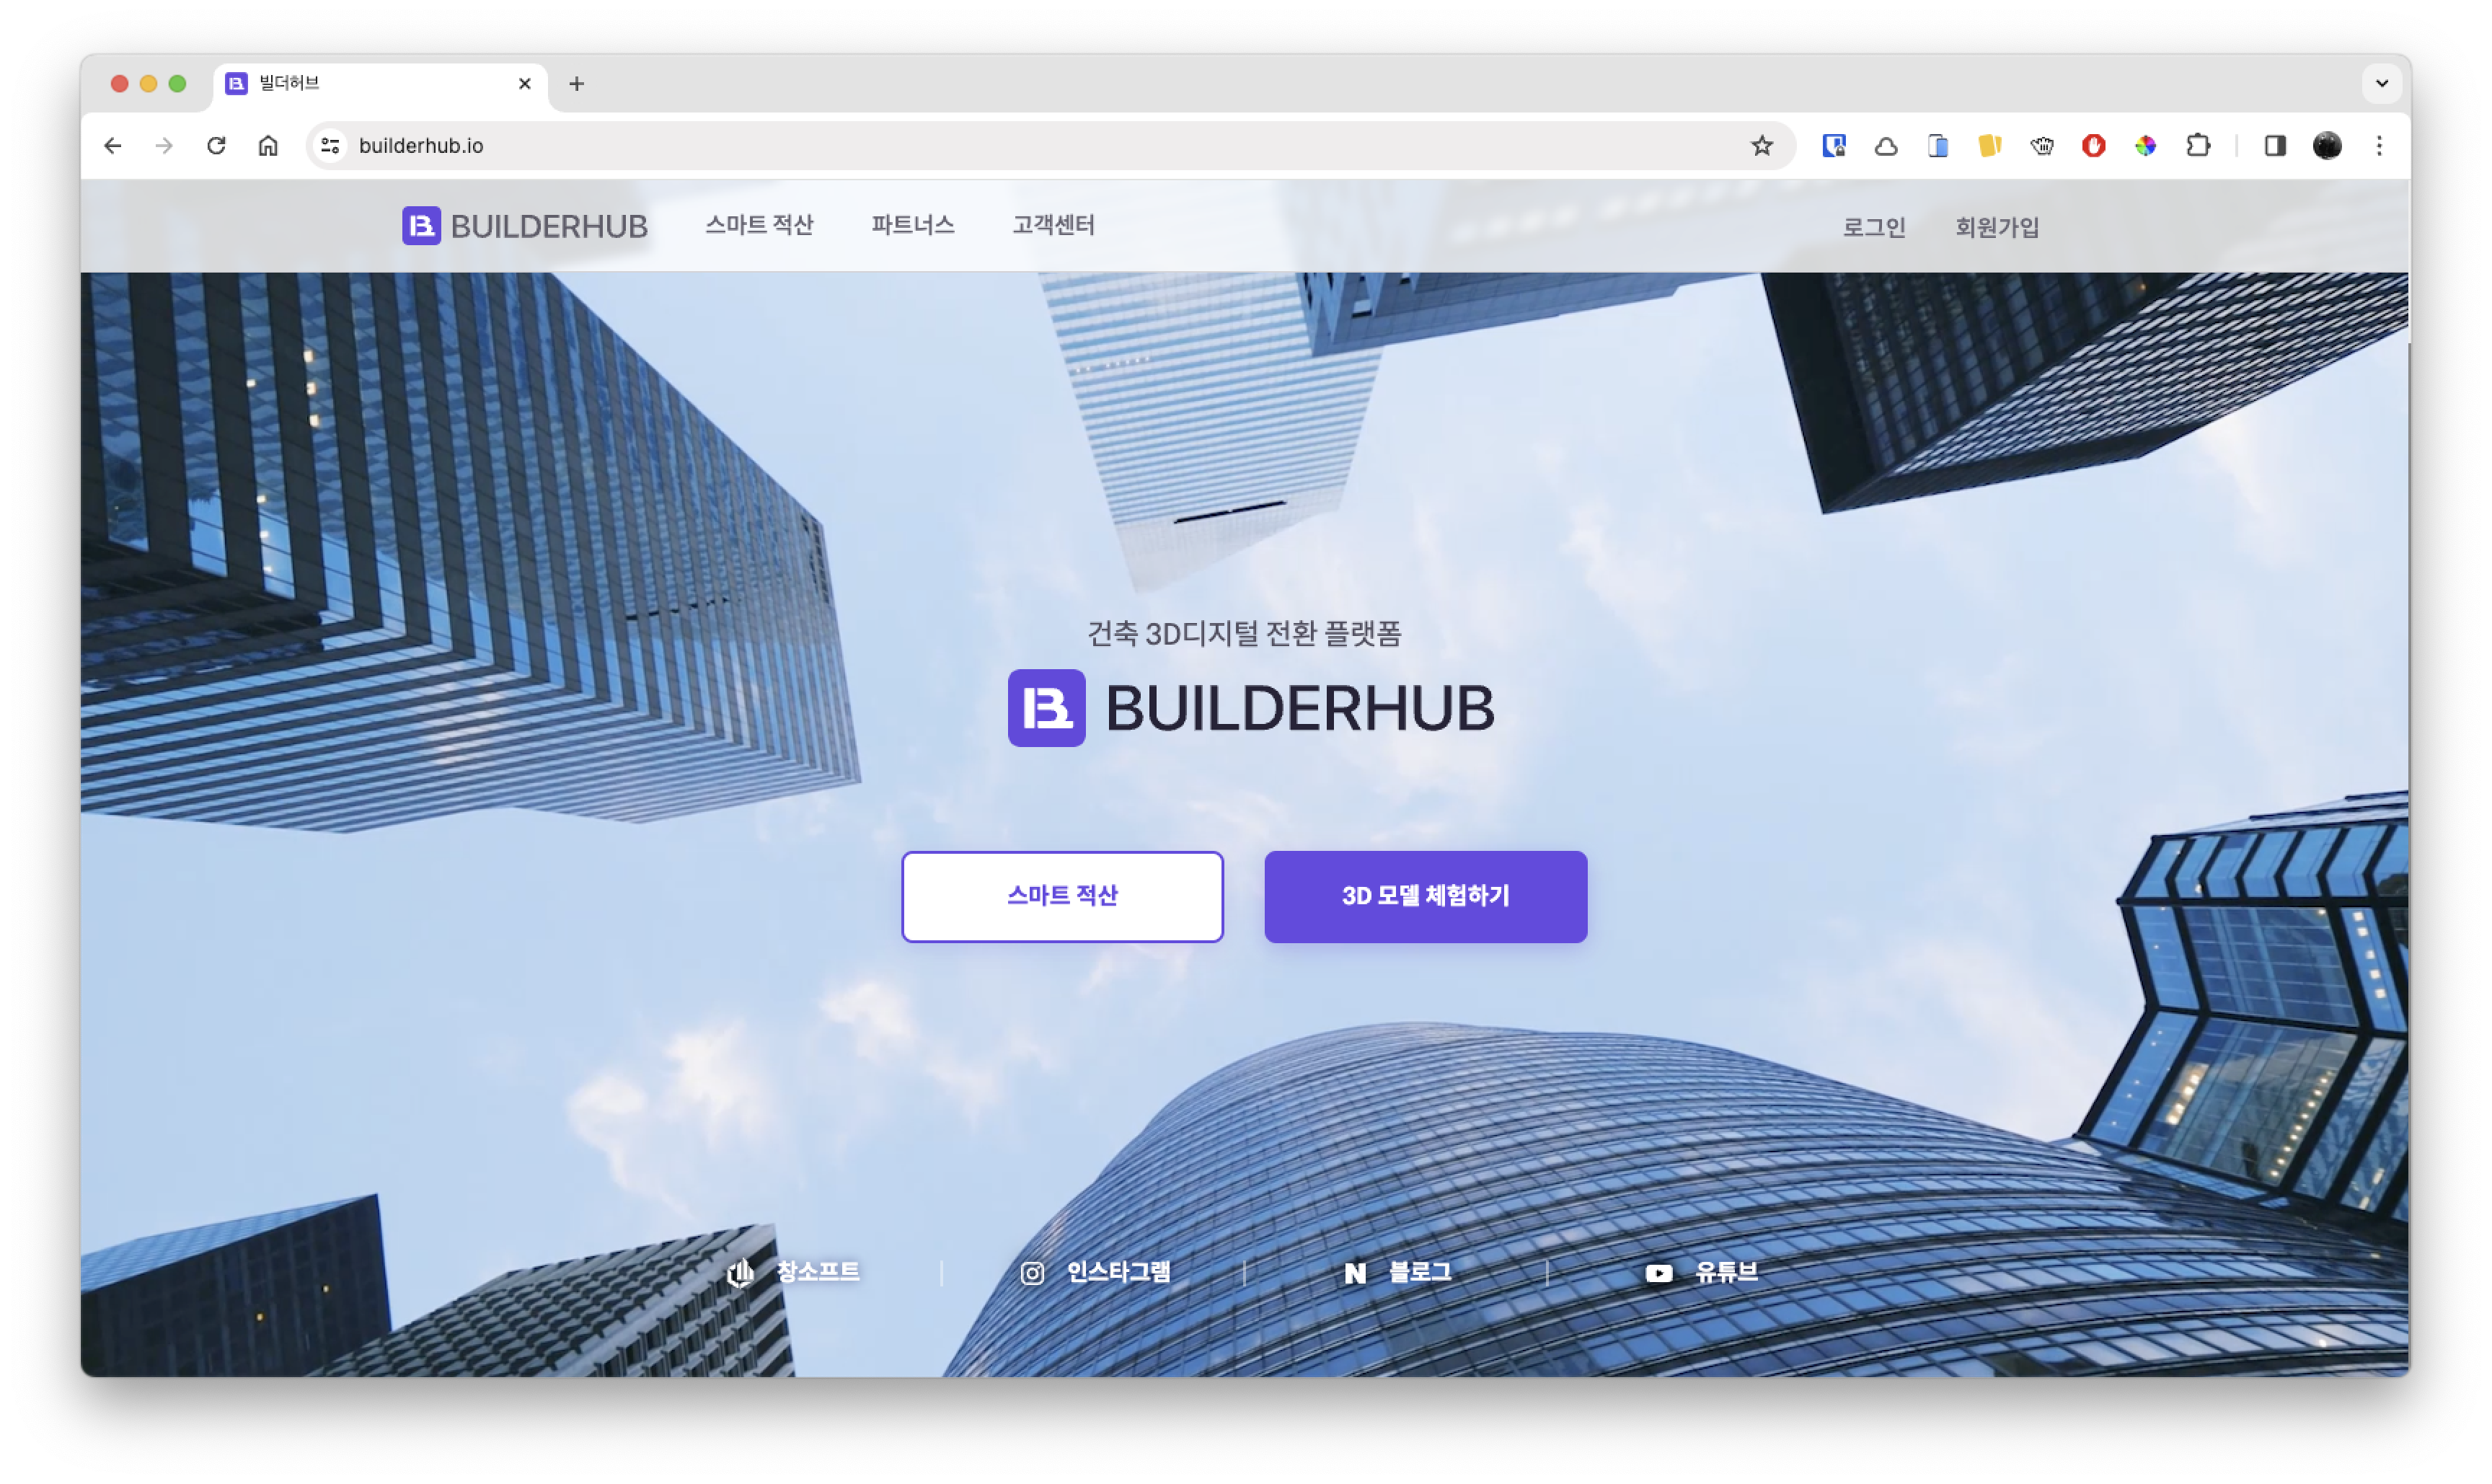
\includegraphics[width=0.35\textwidth]{images/builderhub-home-1.png}
					            \caption*{Builderhub}
				            }\qquad
				            \parbox{0.35\textwidth}{
					            \centering
					            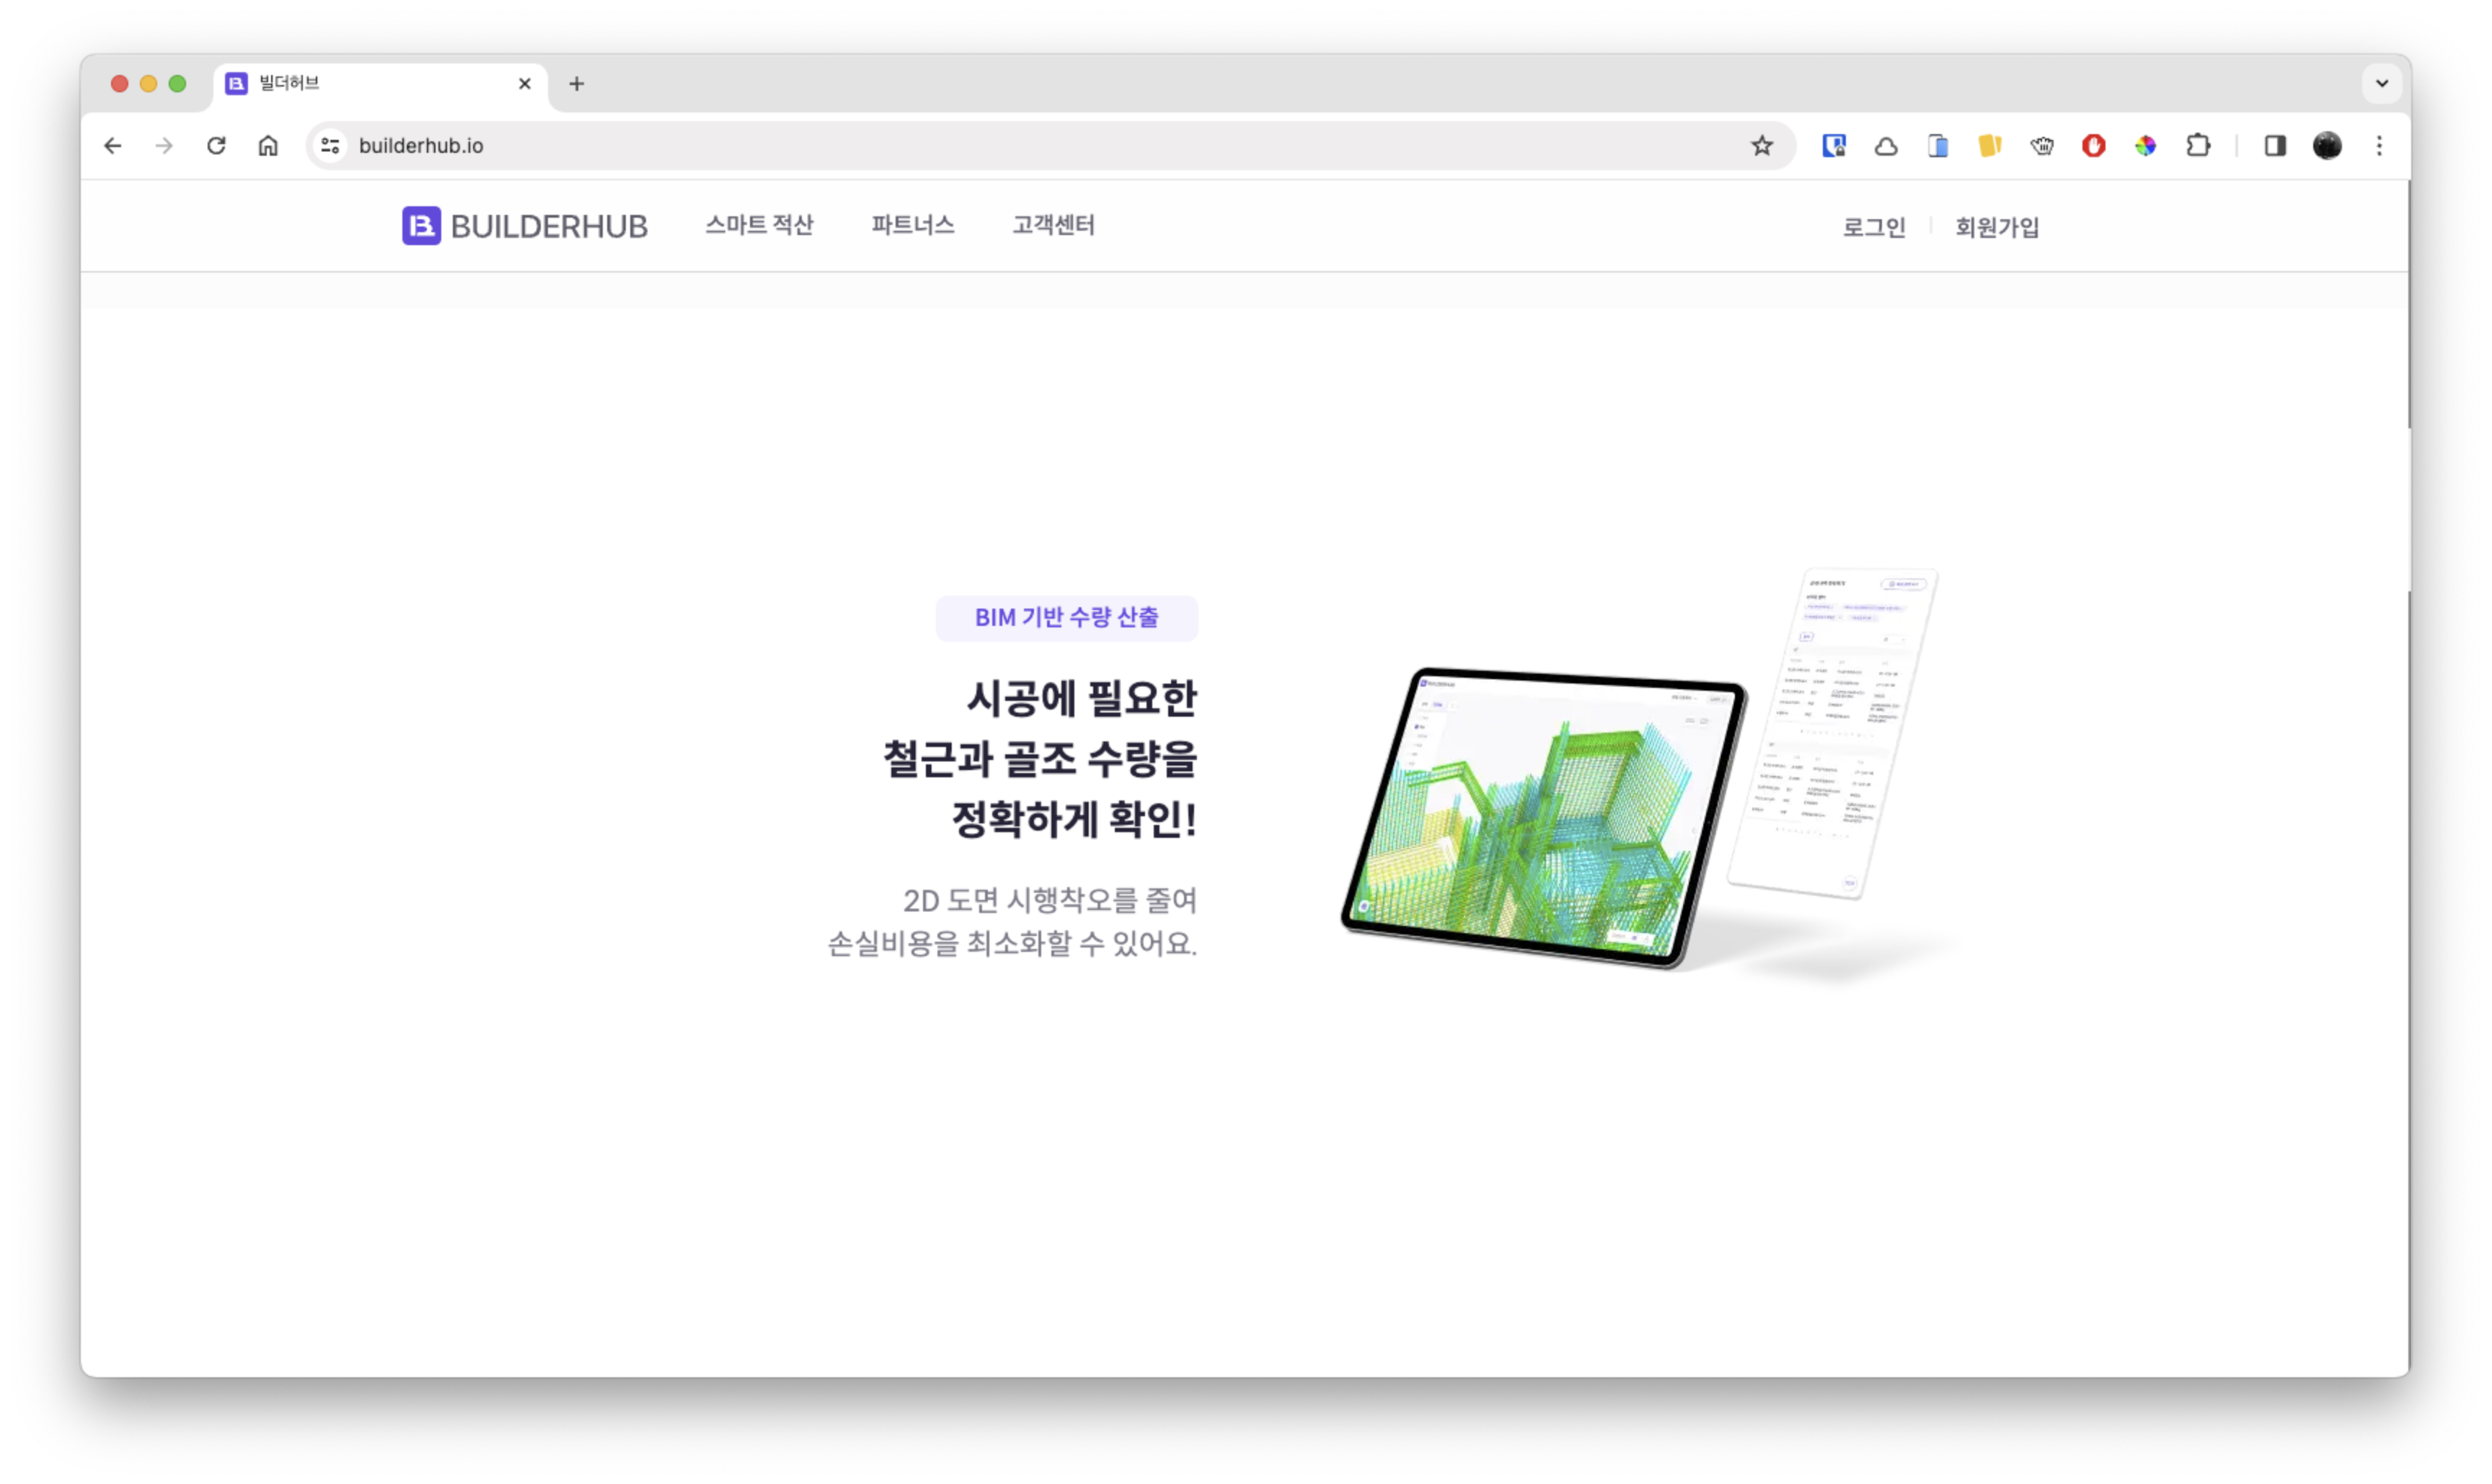
\includegraphics[width=0.35\textwidth]{images/builderhub-home-2.png}
					            \caption*{Home}
				            }\qquad
				            \parbox{0.35\textwidth}{
					            \centering
					            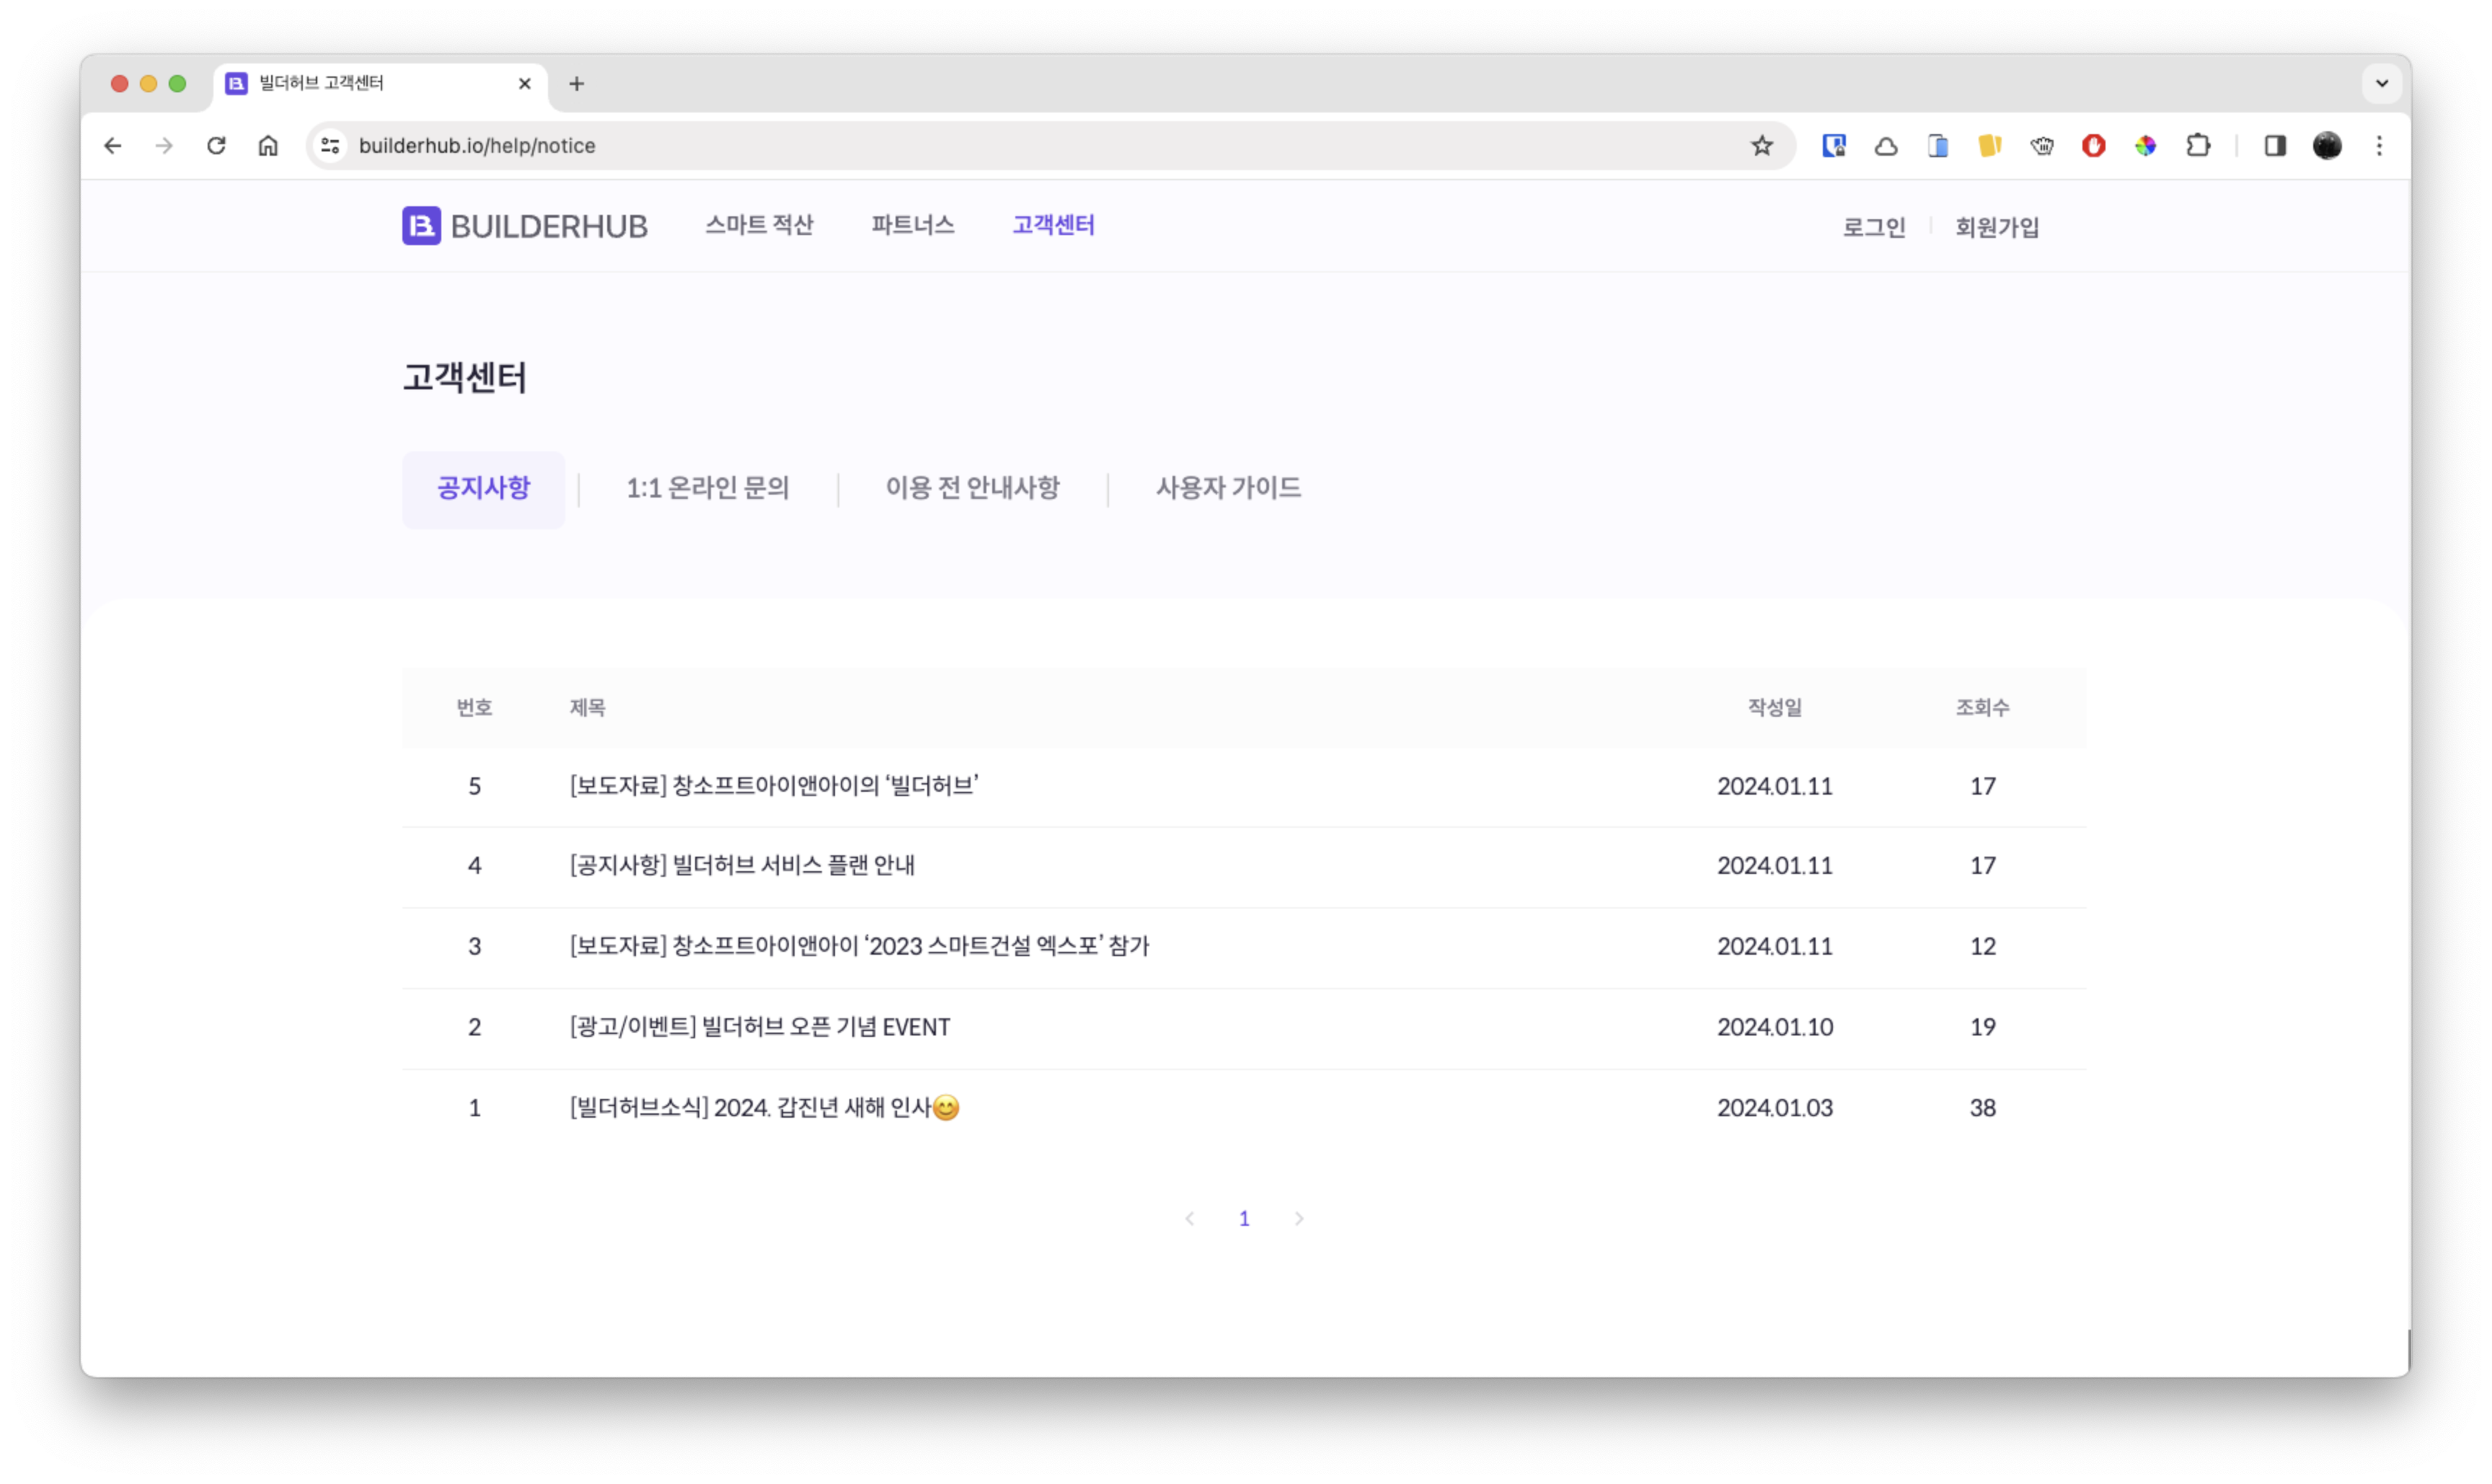
\includegraphics[width=0.35\textwidth]{images/builderhub-home-cs-1.png}
					            \caption*{1:1문의}
				            }\qquad
				            \parbox{0.35\textwidth}{
					            \centering
					            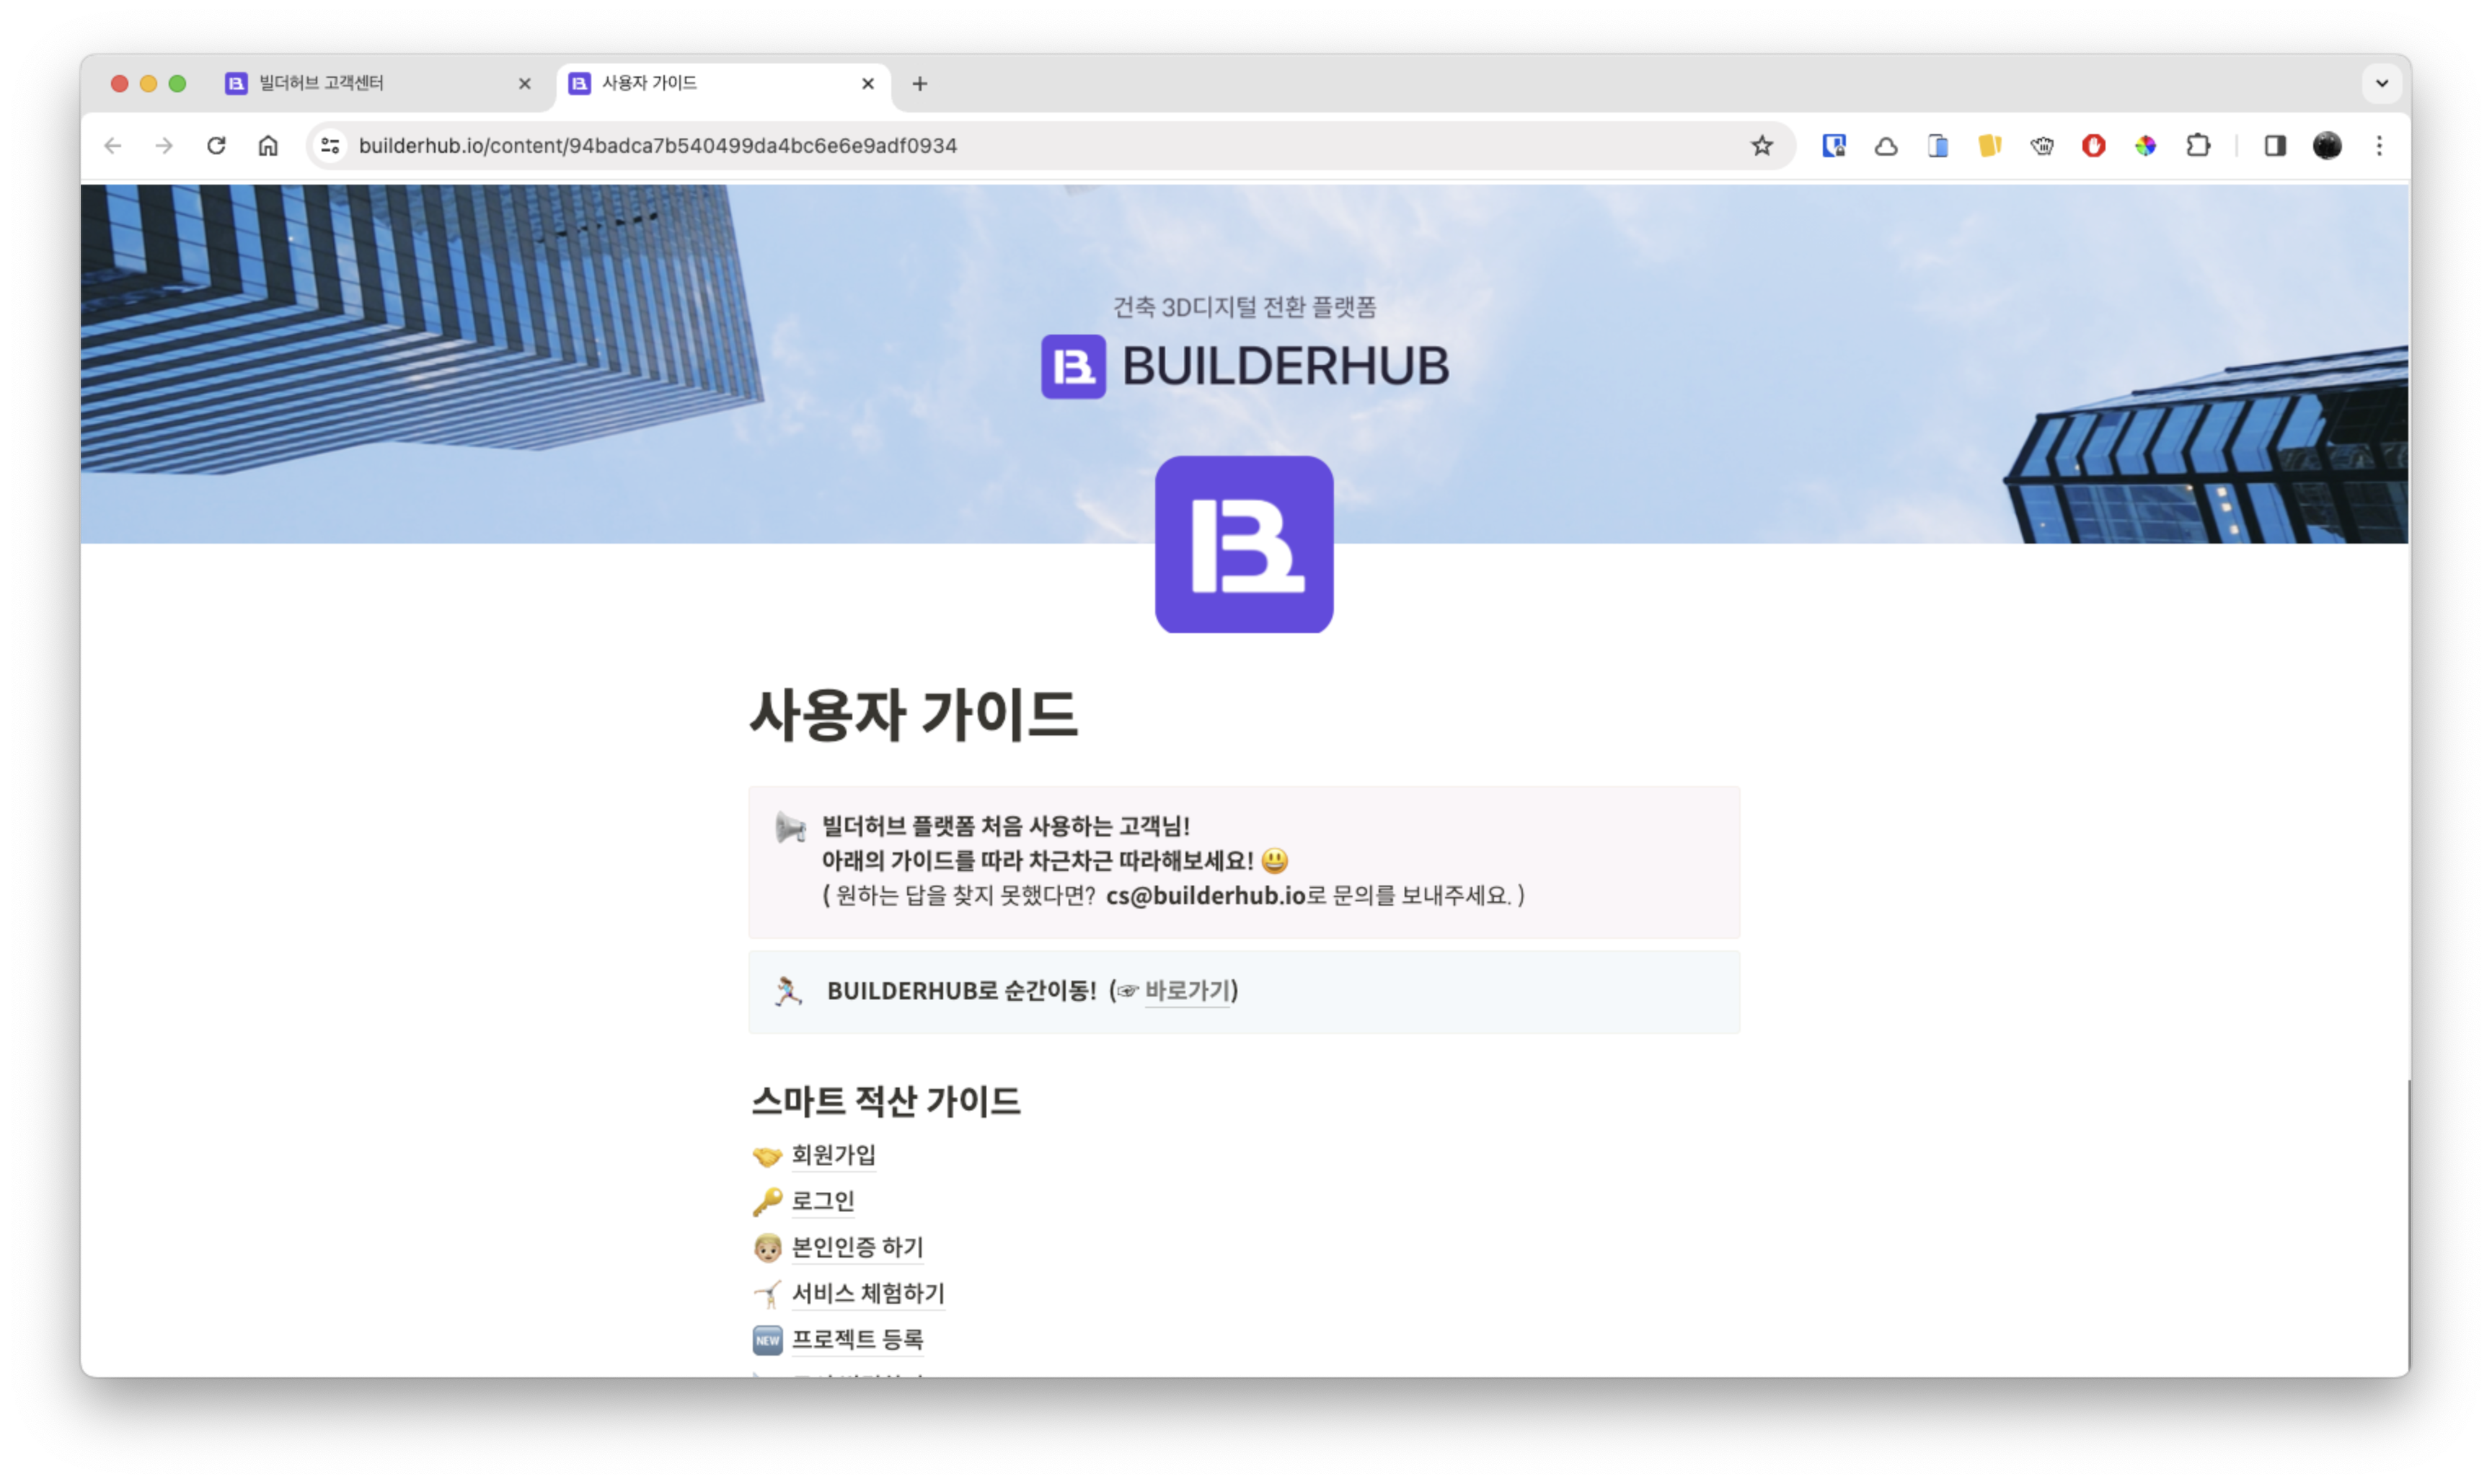
\includegraphics[width=0.35\textwidth]{images/builderhub-home-cs-2.png}
					            \caption*{Guide}
				            }
			            \end{fullwidth}
		            \end{figure}
		      \item \textbf{\href{https://auth.builderhub.io}{인증 서비스} 개발}
		            \begin{itemize}
			            \item 회원가입, 로그인
			            \item 로그인 세션 확인, 마이페이지, 1:1 문의 내역
			            \item SuperTokens(cIAM) API 커스텀, JWT \& Session 방식 인증\&인가, RBAC
		            \end{itemize}
		            \begin{figure}[!ht]
			            \begin{fullwidth}
				            \parbox{0.5\textwidth}{
					            \centering
					            \includegraphics[width=0.5\textwidth]{images/builderhub-auth-1.png}
					            \caption*{Sign in}
				            }\qquad
				            \parbox{0.5\textwidth}{
					            \centering
					            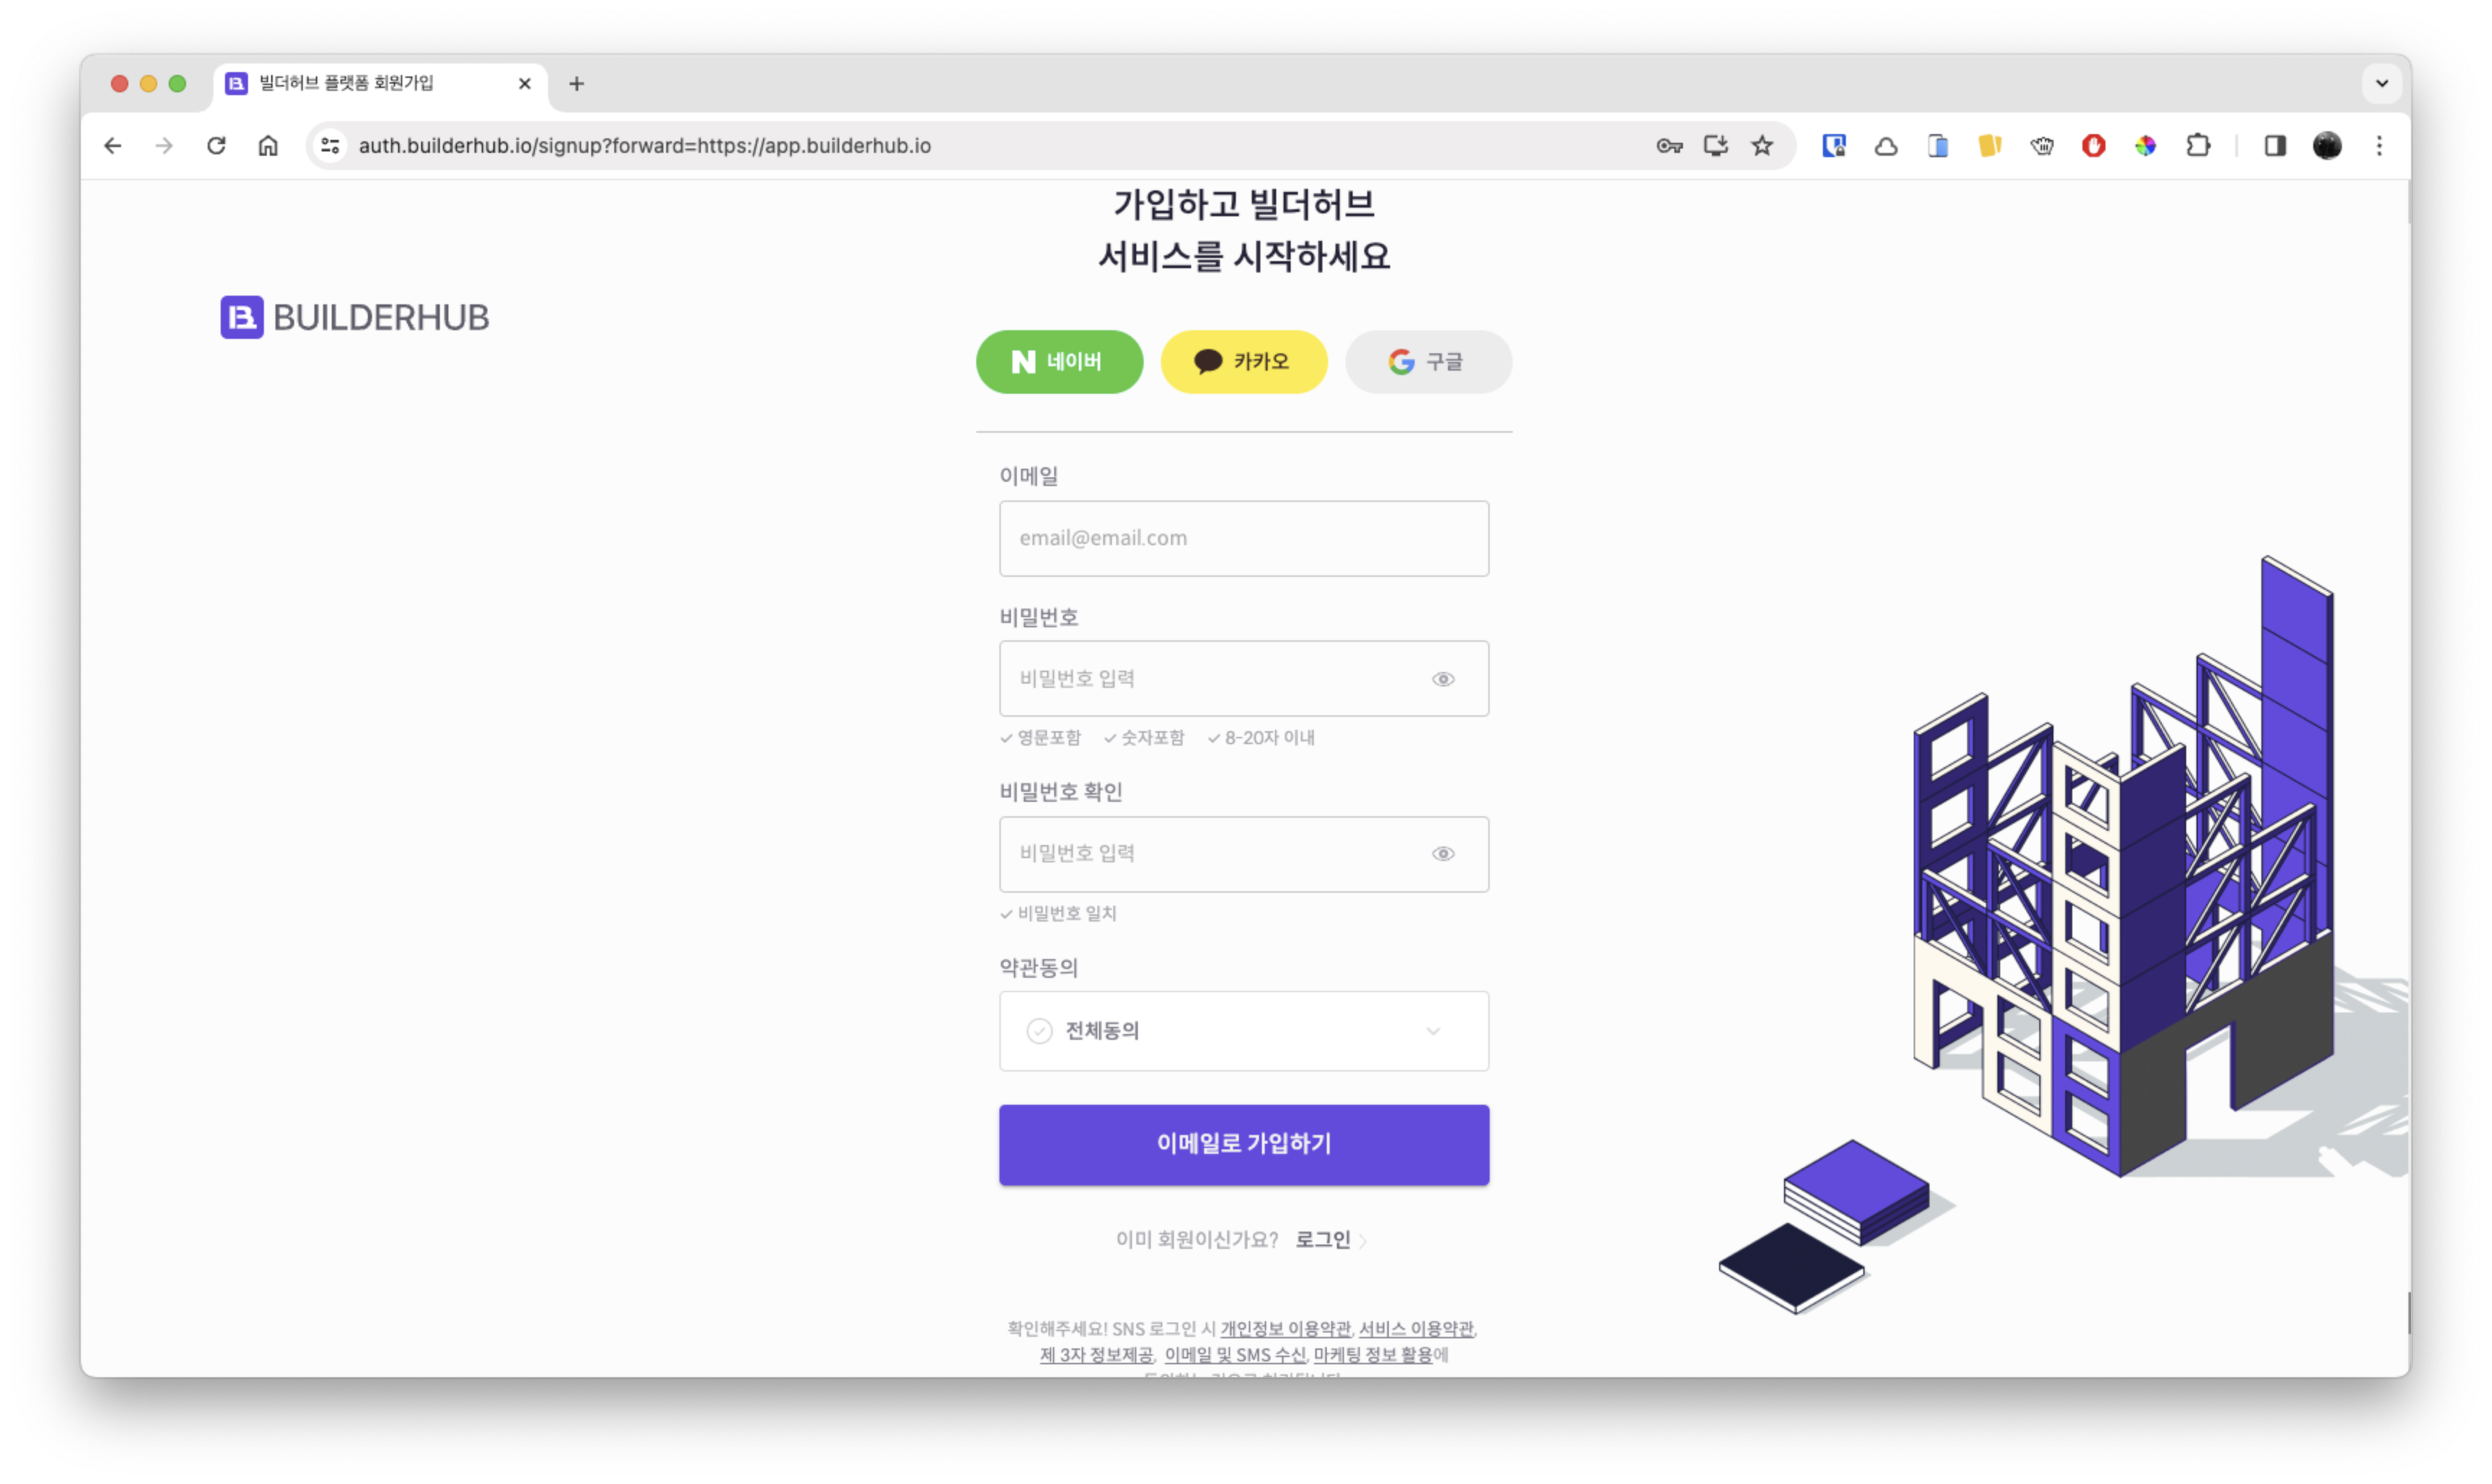
\includegraphics[width=0.5\textwidth]{images/builderhub-auth-2.png}
					            \caption*{Sign up}
				            }\qquad
				            \parbox{0.5\textwidth}{
					            \centering
					            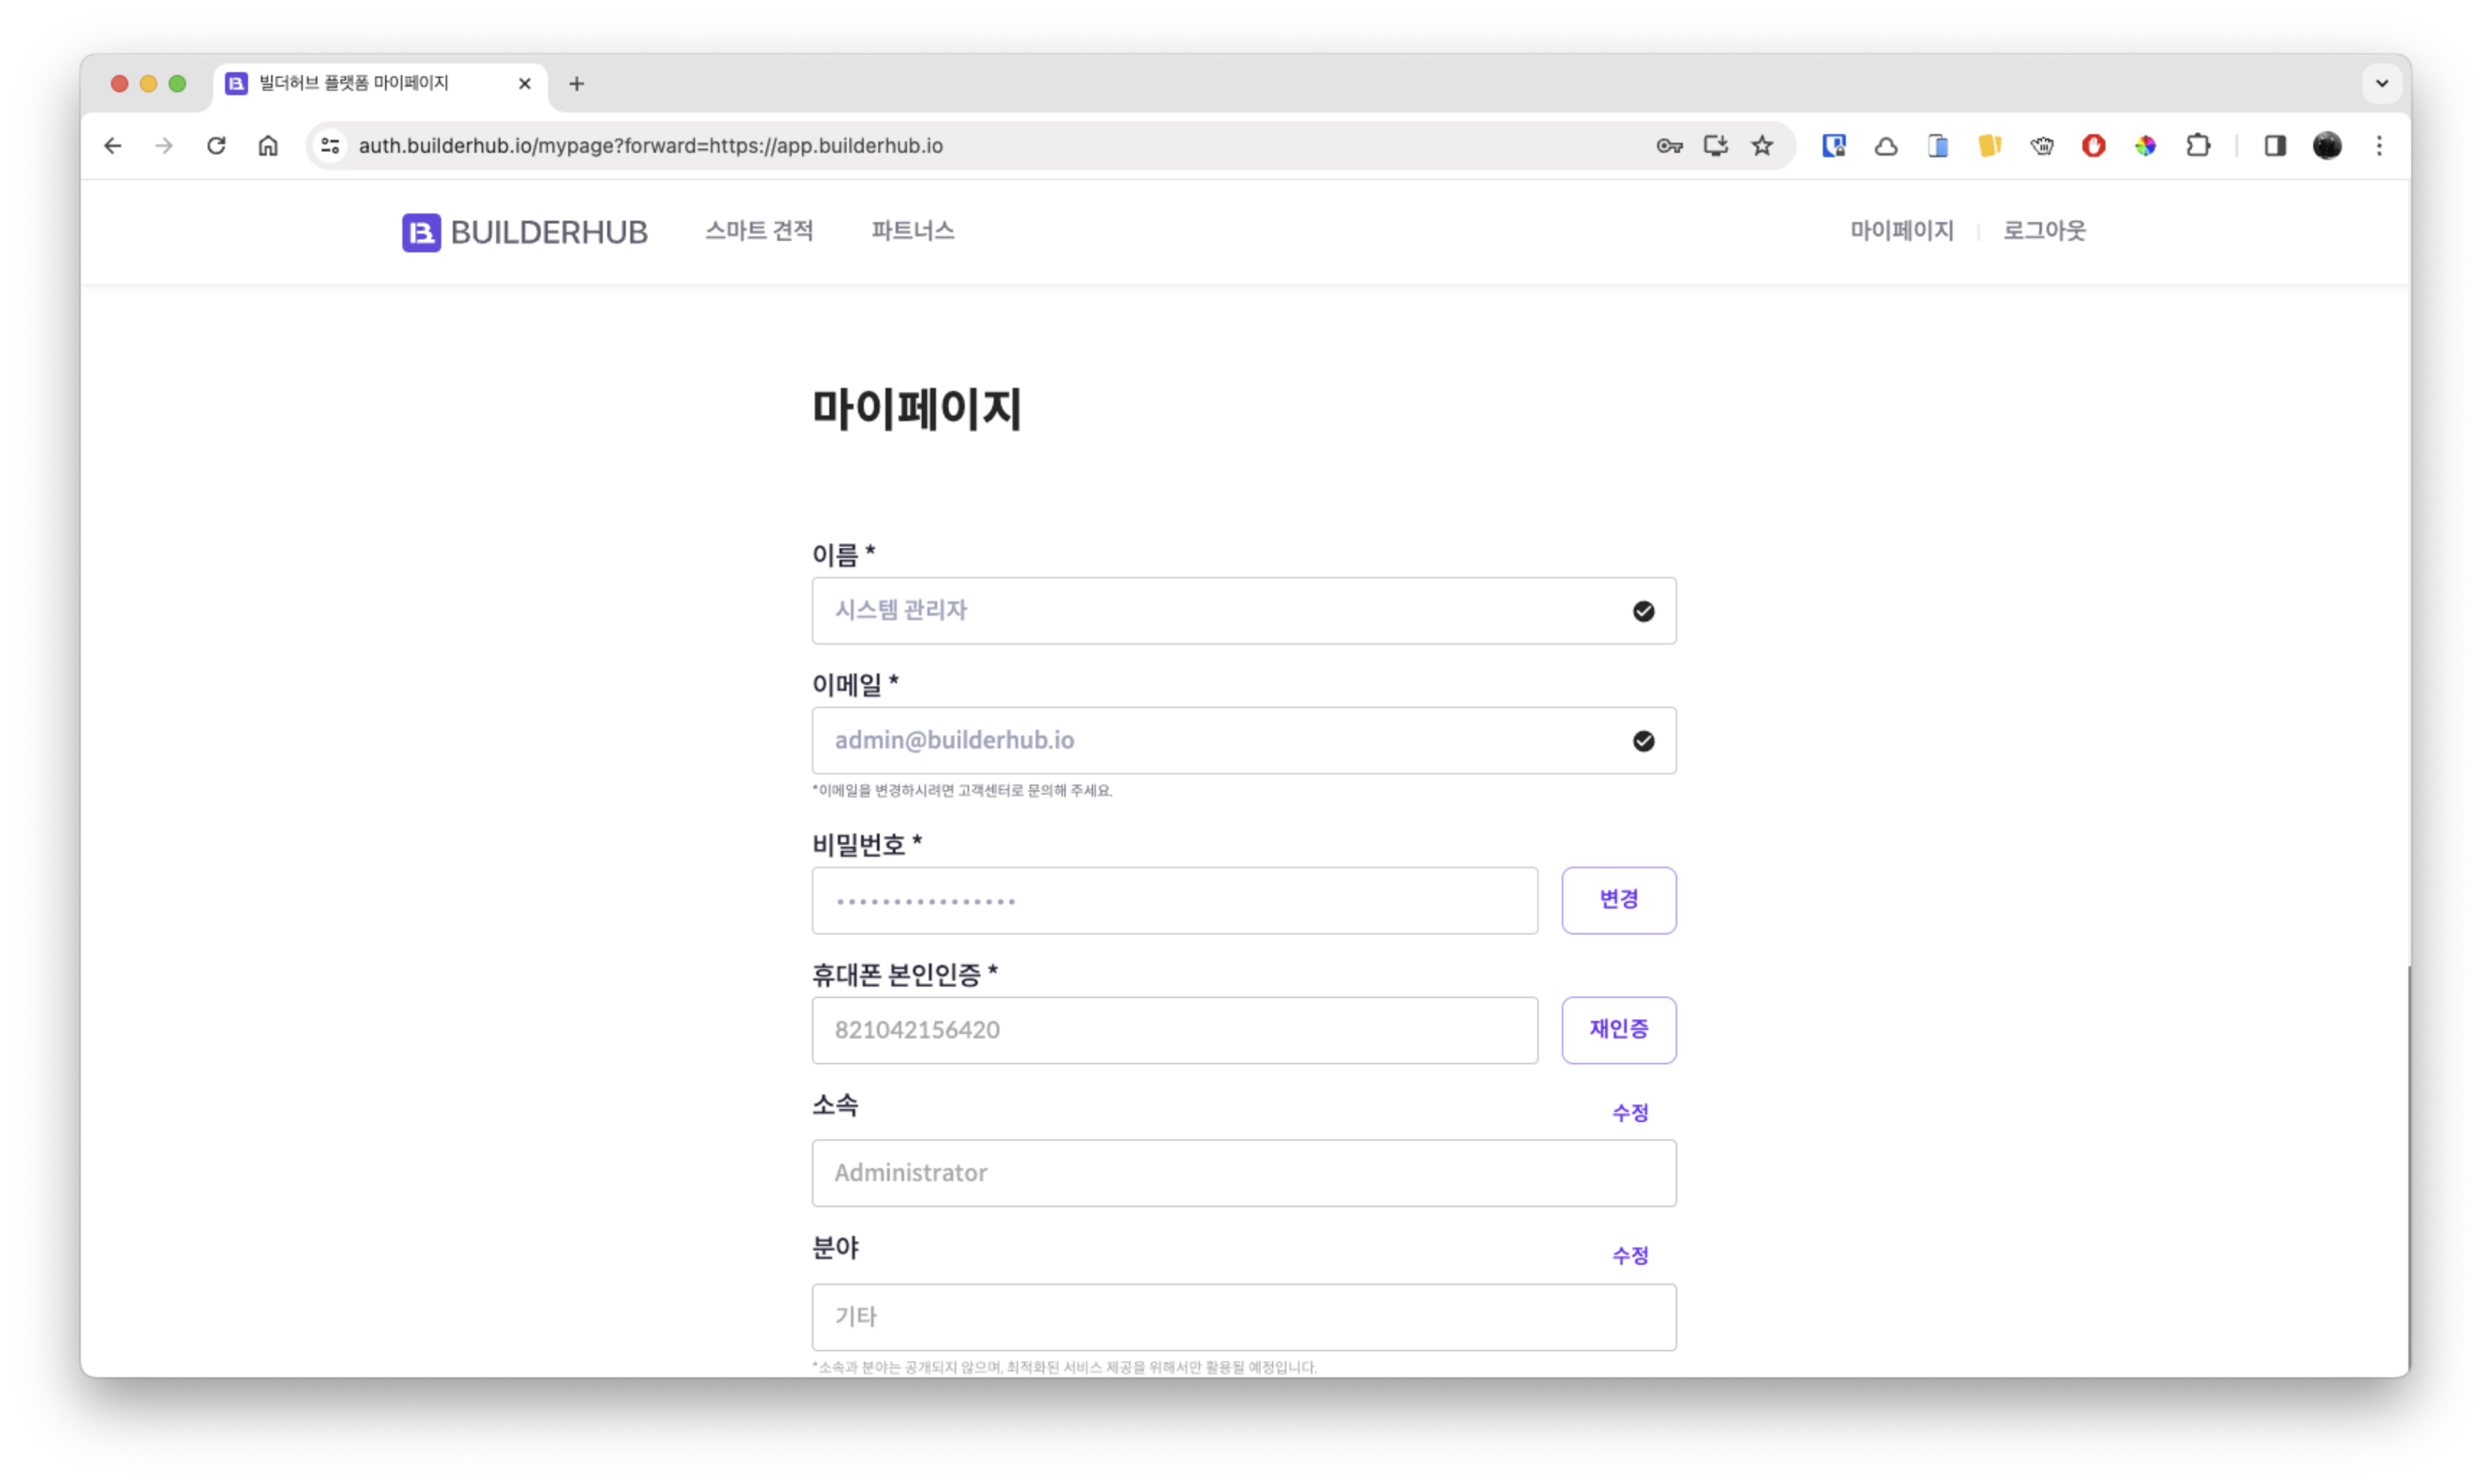
\includegraphics[width=0.5\textwidth]{images/builderhub-auth-mypage.png}
					            \caption*{My Page}
				            }
			            \end{fullwidth}
		            \end{figure}
		      \item \textbf{\href{https://app.builderhub.io}{커스터머 서비스} 개발}
		            \begin{itemize}
			            \item 랜딩페이지, 프로젝트 리스트, 등록, 공유, 필터
			            \item 프로젝트 상태 확인, 결제 시스템, 알림톡 연동
			            \item 프로젝트 상세 확인, 변경 내역 히스토리
			            \item 표준내역서 관리, 내역화 (개발중)
		            \end{itemize}
		            \begin{figure}[!ht]
			            \begin{fullwidth}
				            \parbox{0.35\textwidth}{
					            \centering
					            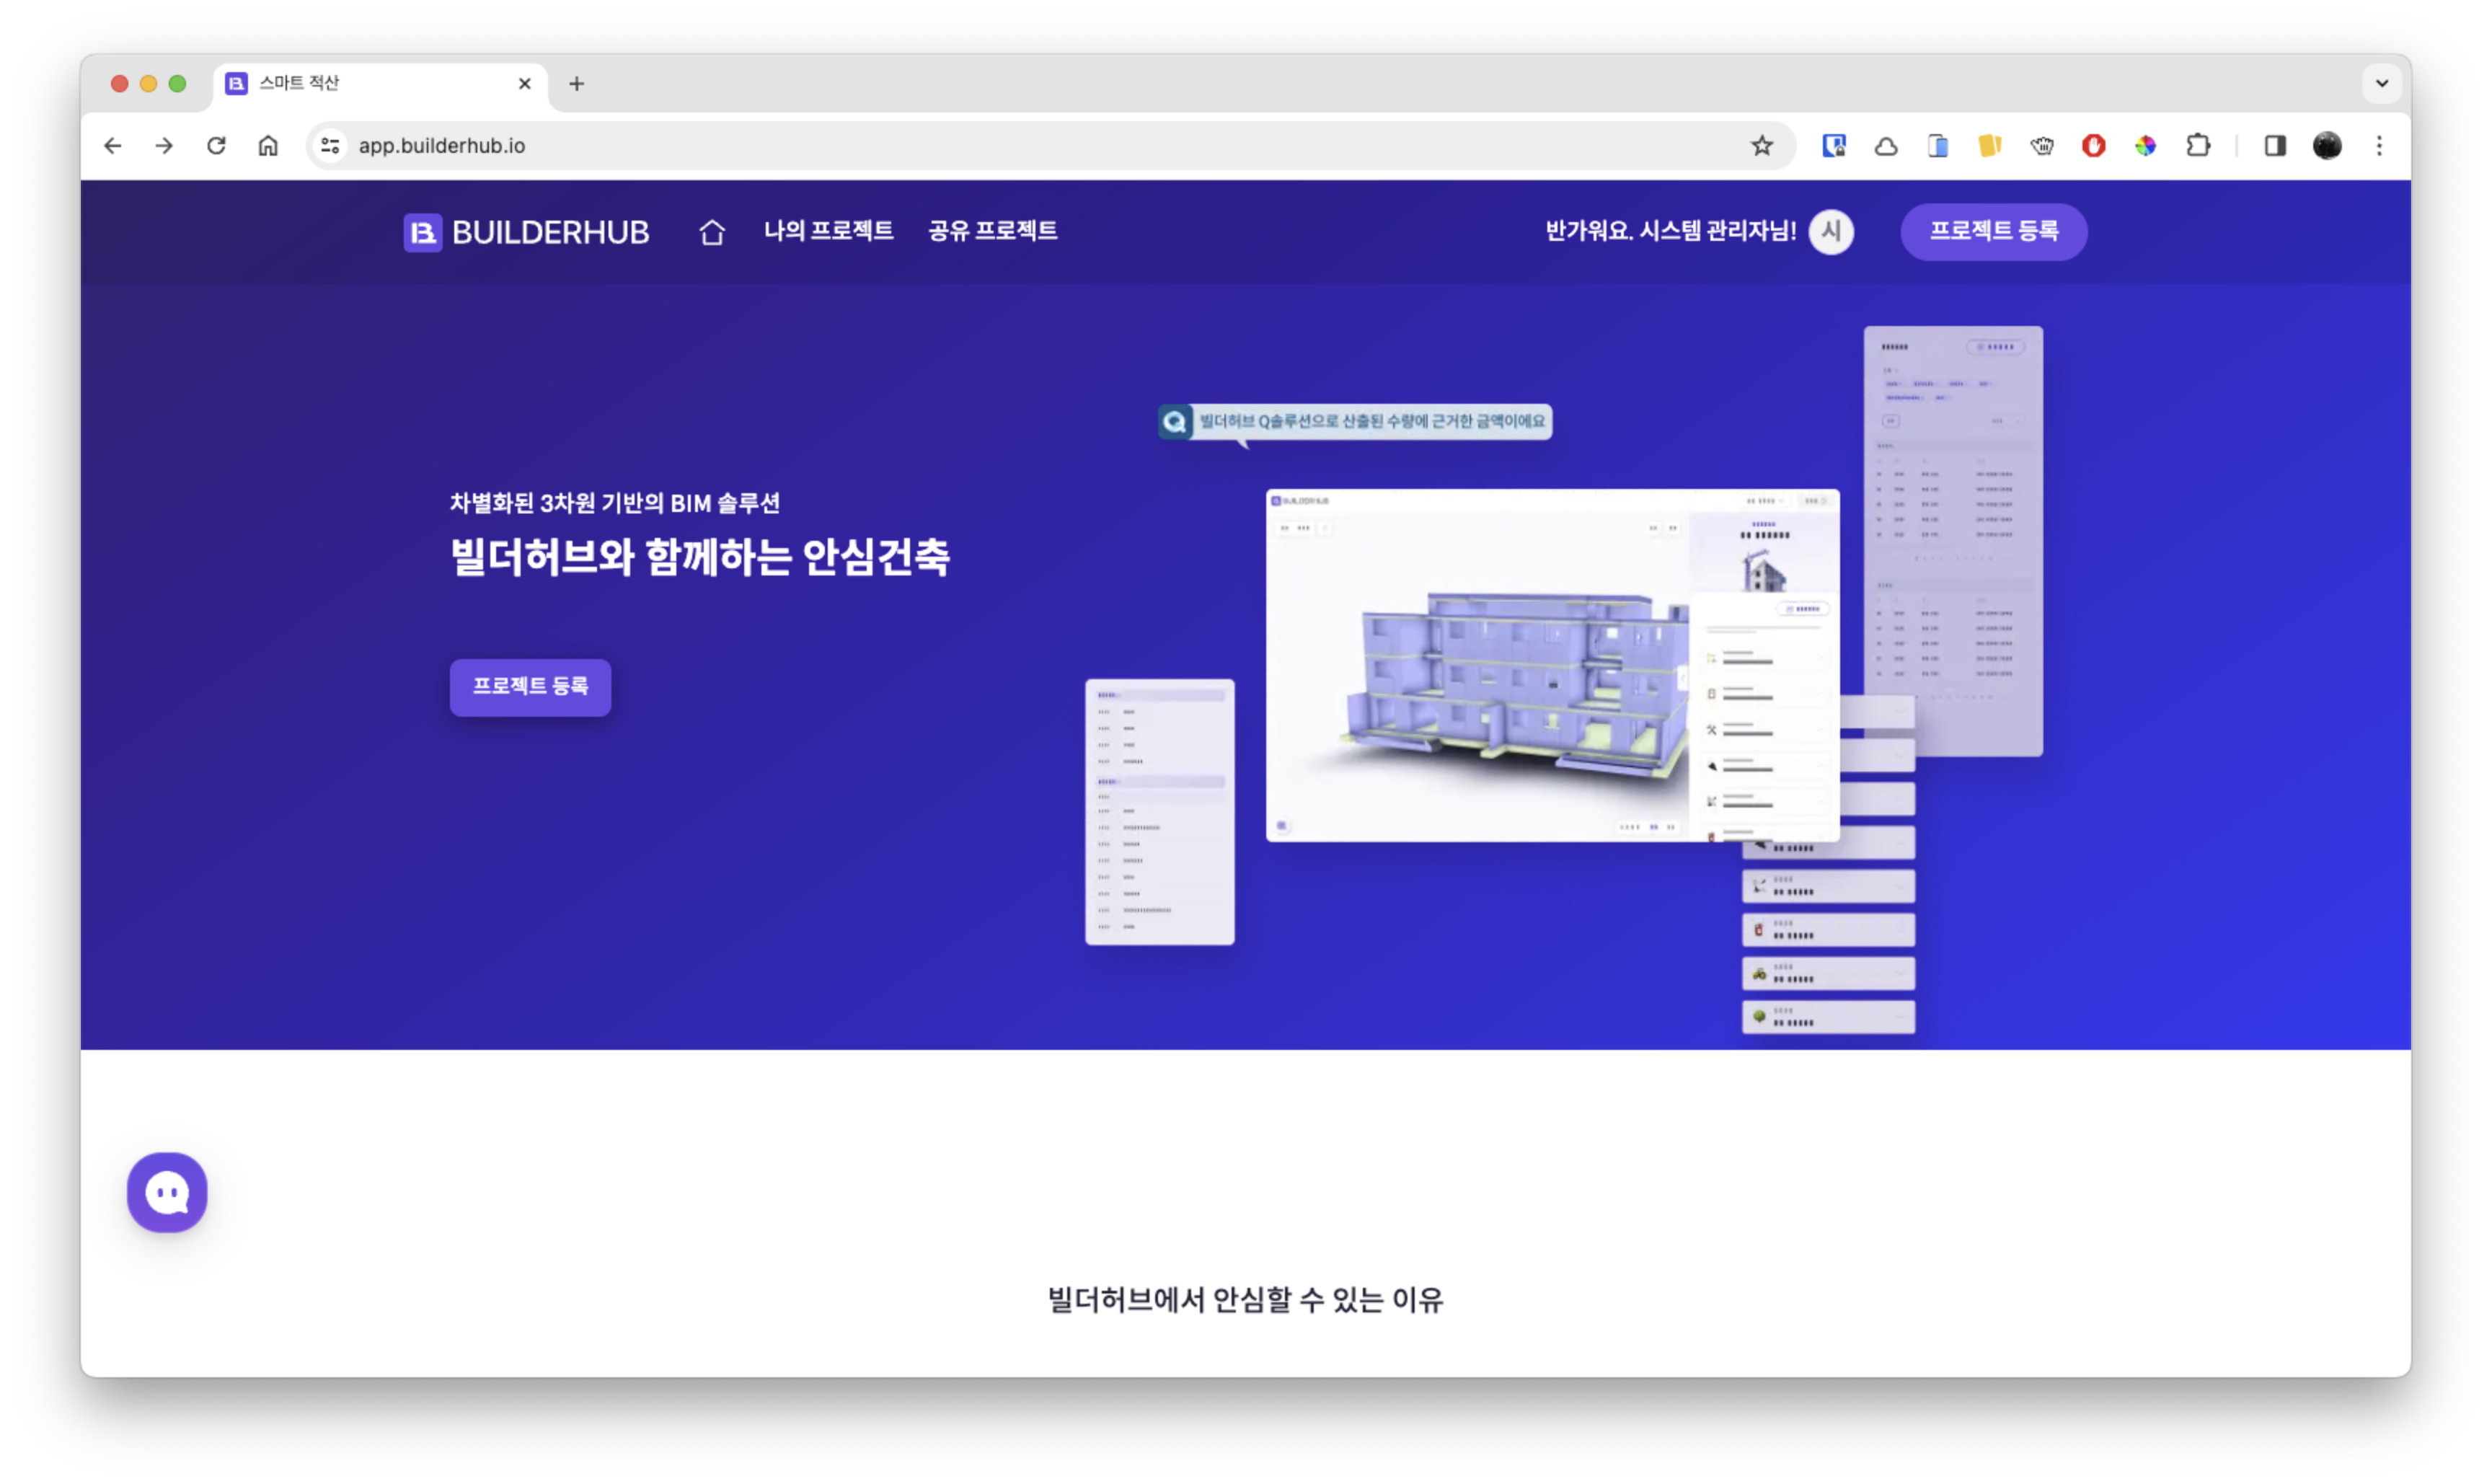
\includegraphics[width=0.35\textwidth]{images/builderhub-customer-1.png}
					            \caption*{Landing page}
				            }\qquad
				            \parbox{0.35\textwidth}{
					            \centering
					            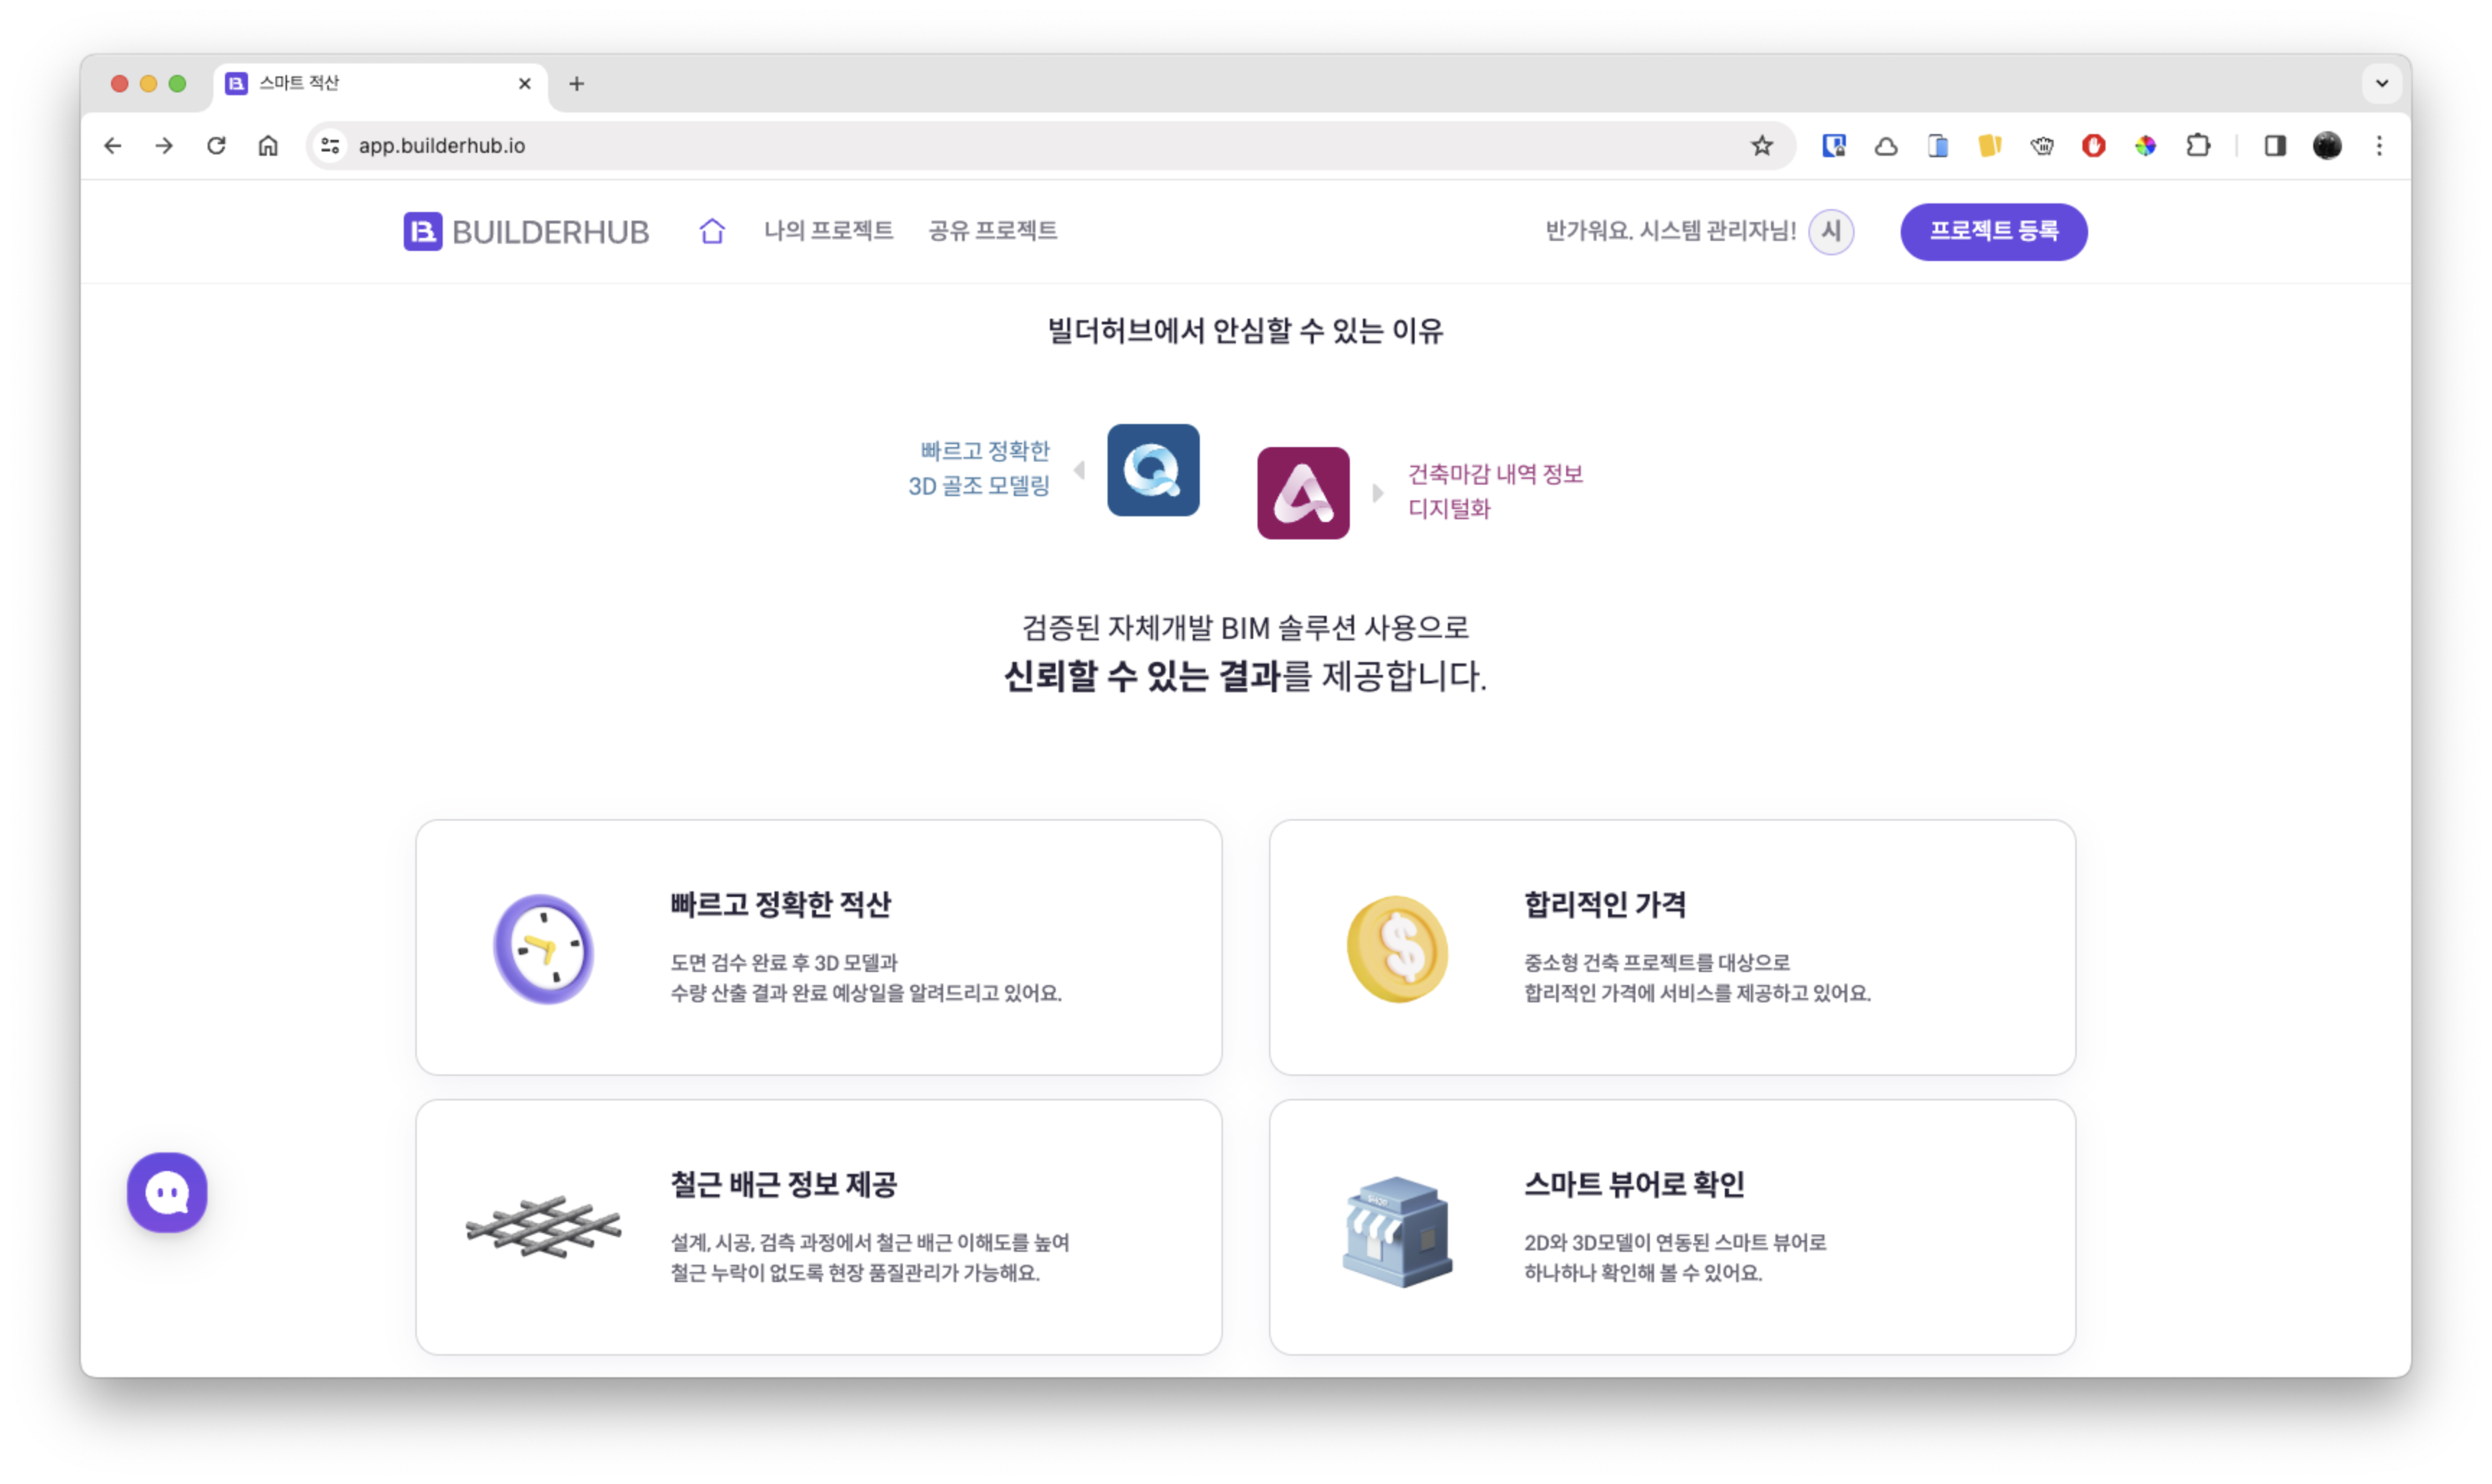
\includegraphics[width=0.35\textwidth]{images/builderhub-customer-2.png}
					            \caption*{Scroll base story telling}
				            }\qquad
				            \parbox{0.35\textwidth}{
					            \centering
					            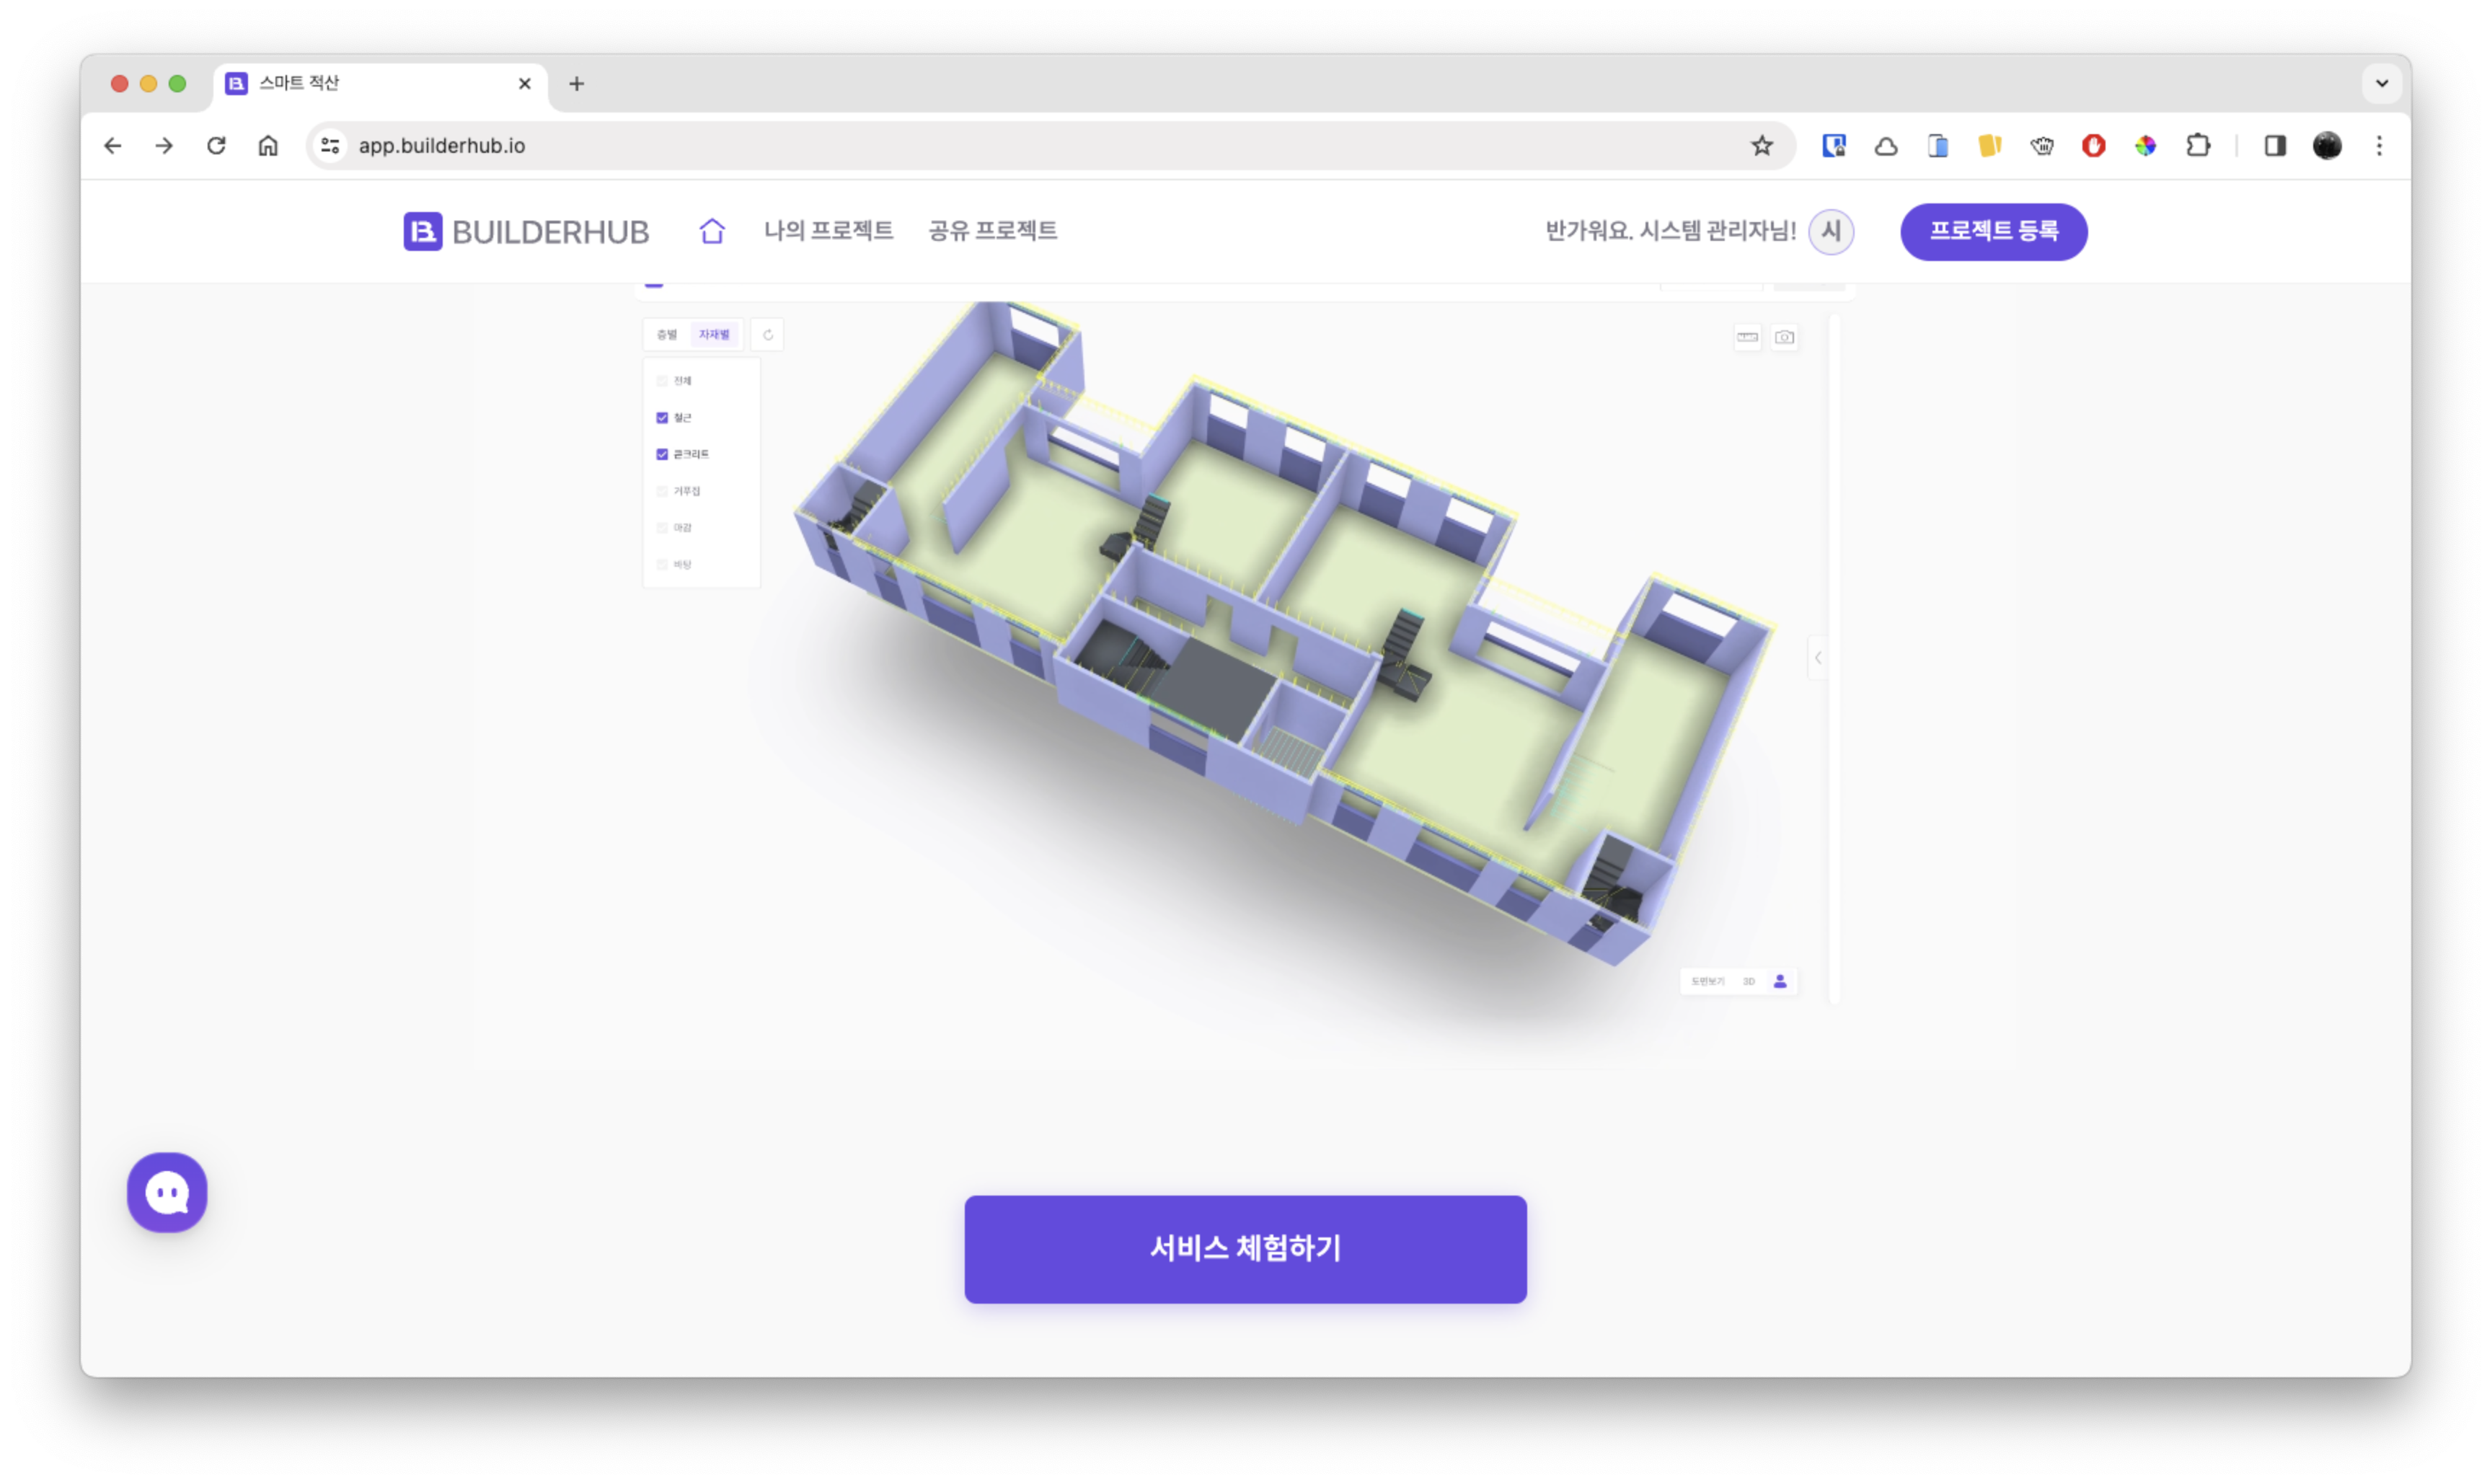
\includegraphics[width=0.35\textwidth]{images/builderhub-customer-3.png}
					            \caption*{Demo}
				            }\qquad
				            \parbox{0.35\textwidth}{
					            \centering
					            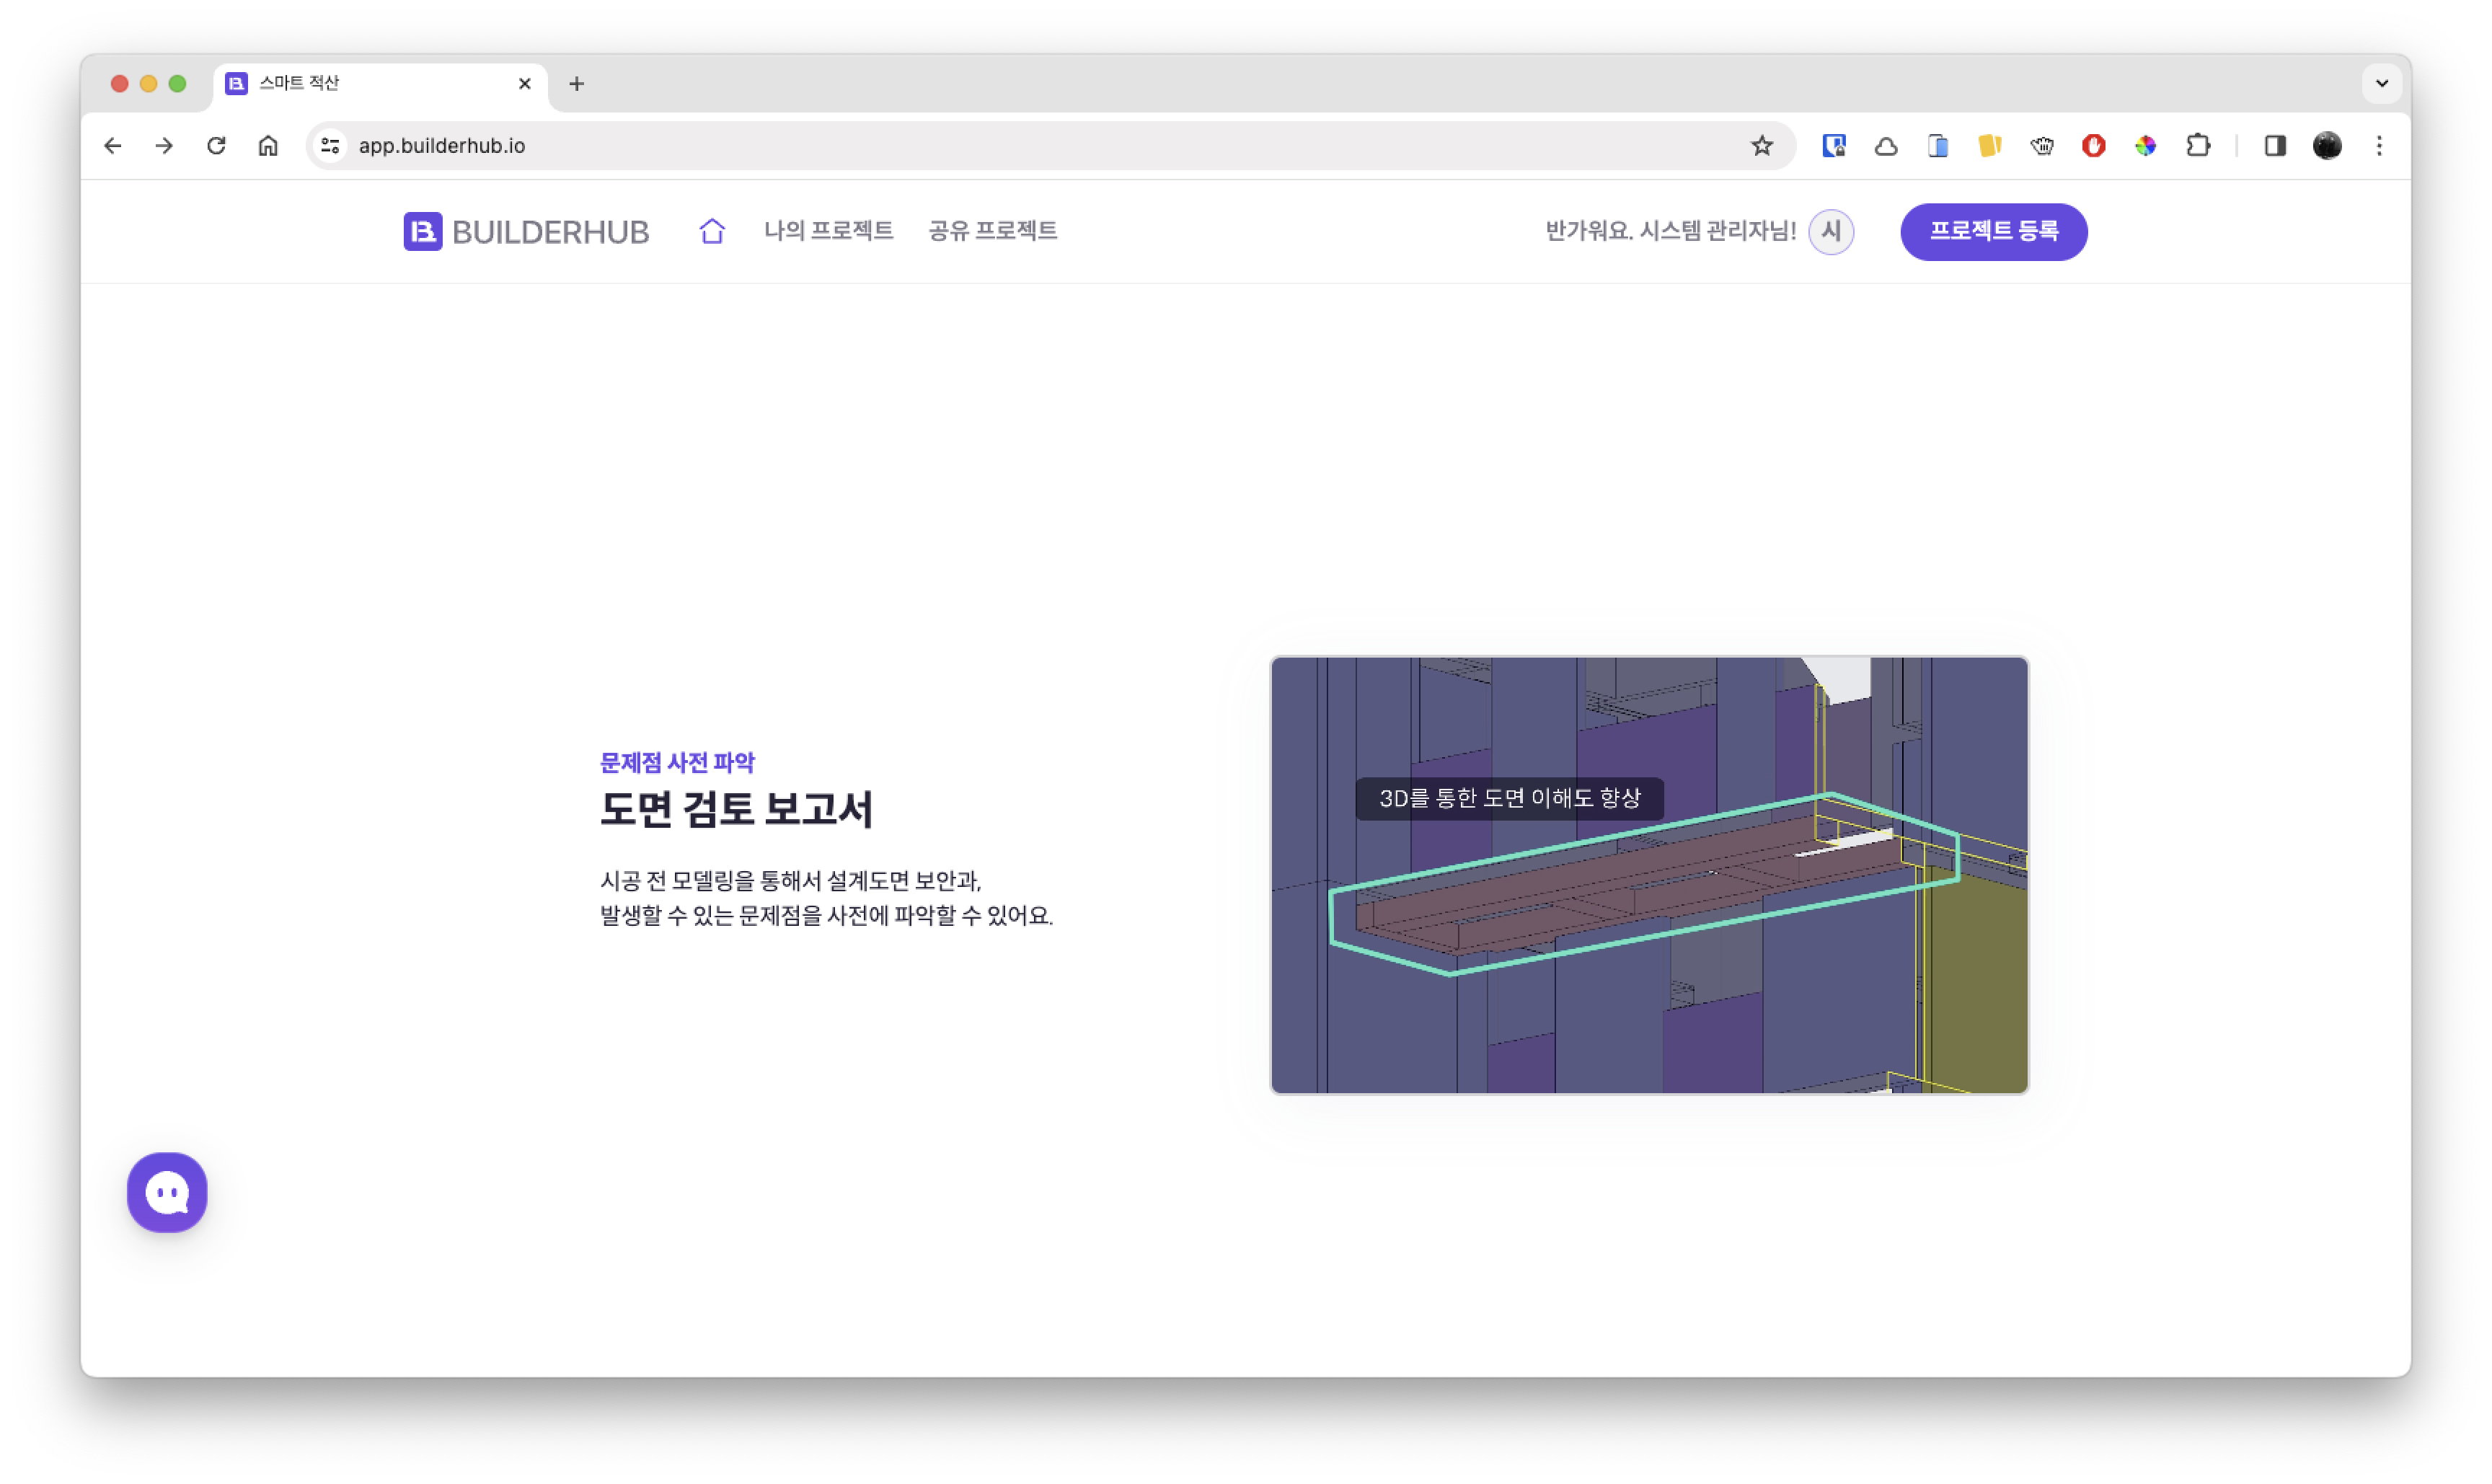
\includegraphics[width=0.35\textwidth]{images/builderhub-customer-4.png}
					            \caption*{Check drawing}
				            }
				            \parbox{0.35\textwidth}{
					            \centering
					            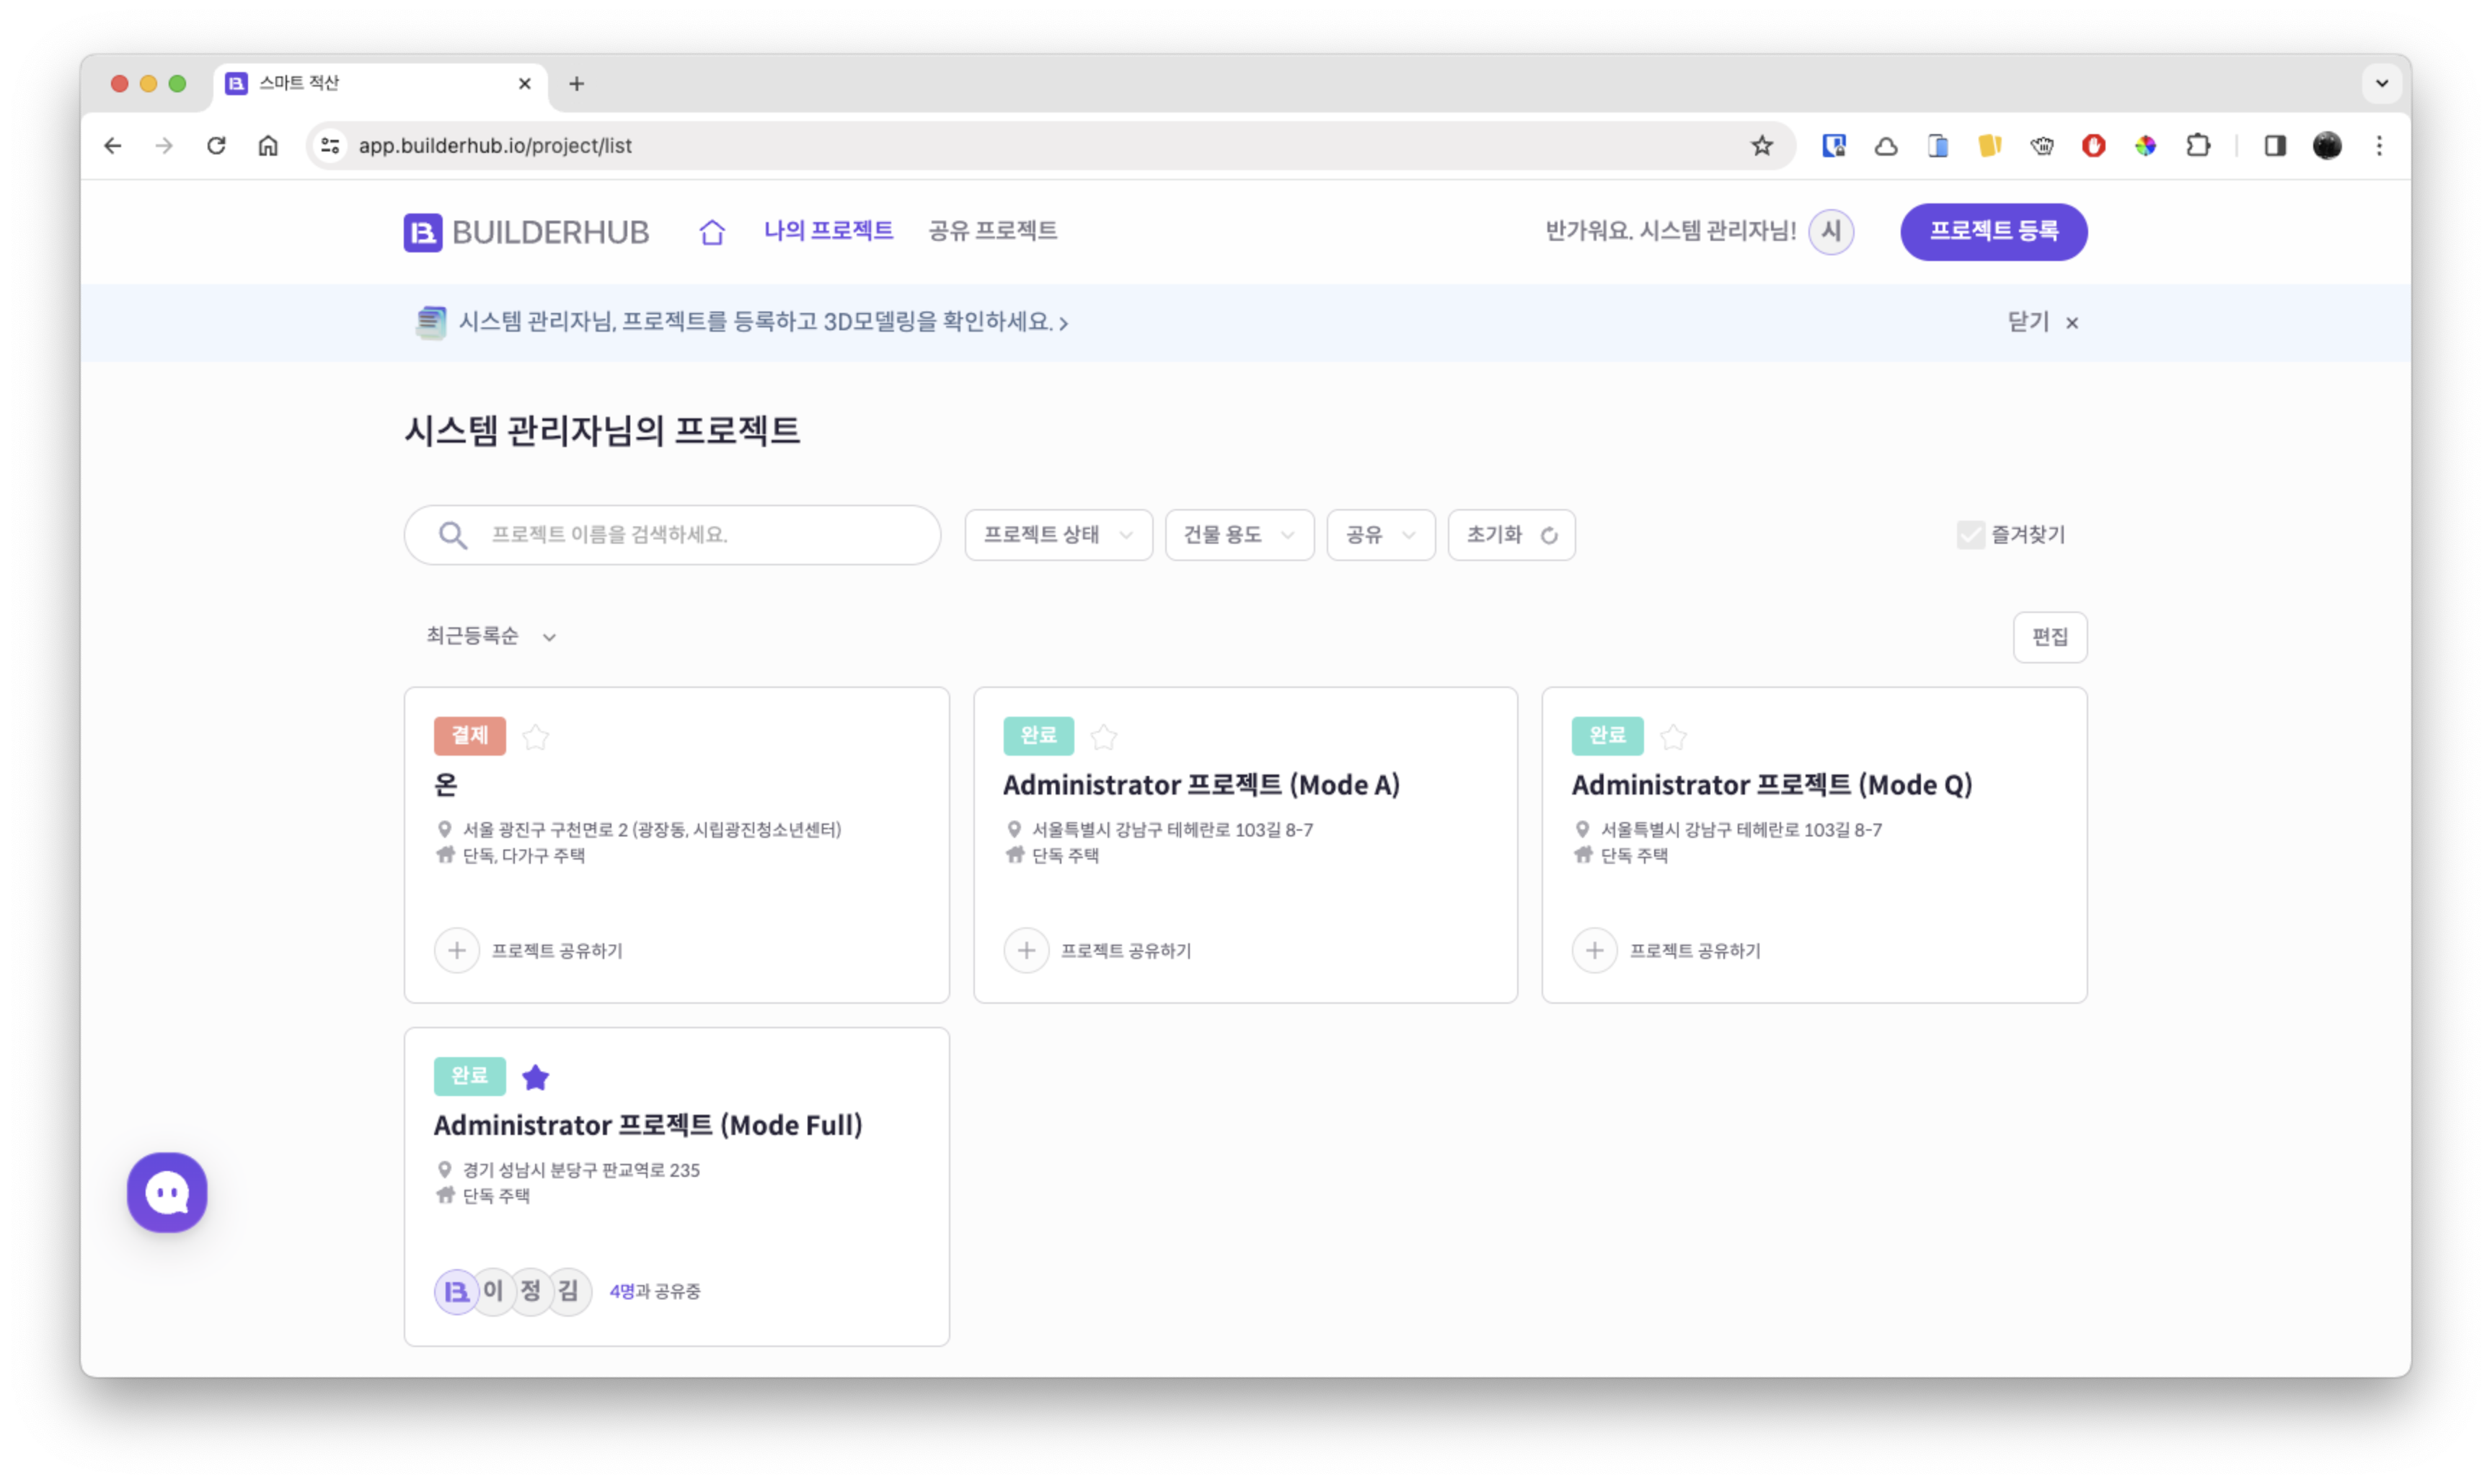
\includegraphics[width=0.35\textwidth]{images/builderhub-customer-project-1.png}
					            \caption*{Project list}
				            }\qquad
				            \parbox{0.35\textwidth}{
					            \centering
					            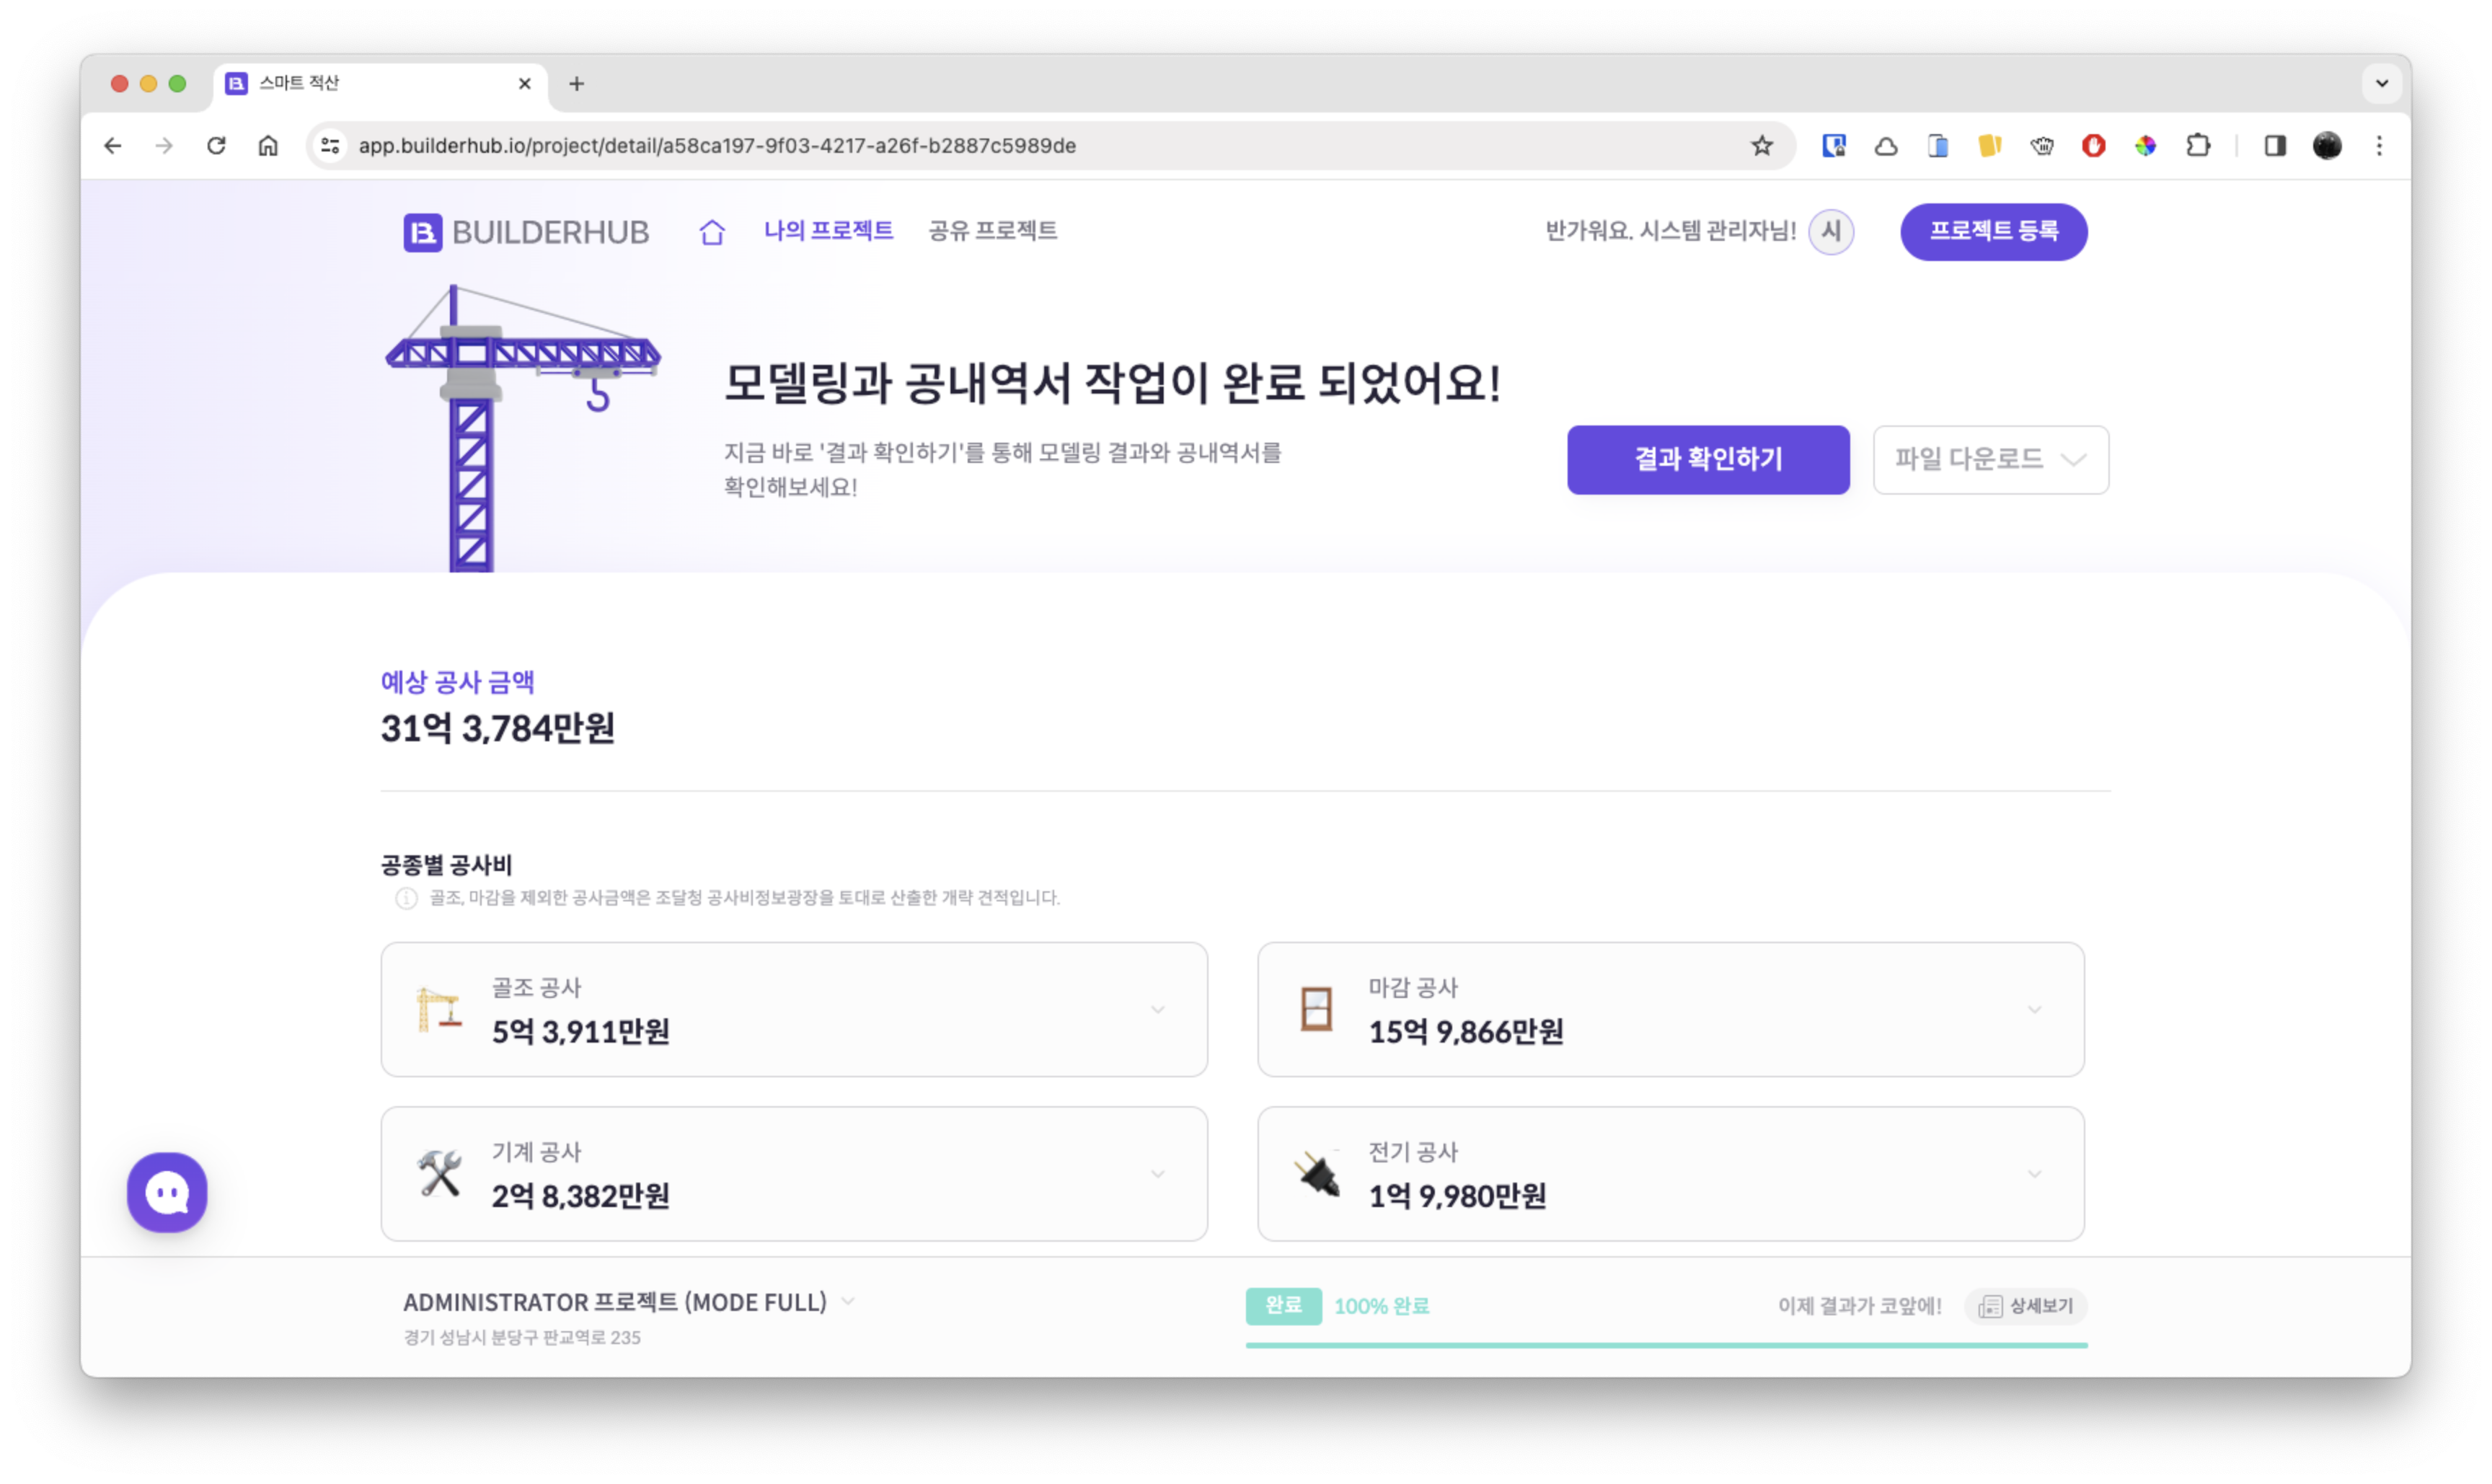
\includegraphics[width=0.35\textwidth]{images/builderhub-customer-project-2.png}
					            \caption*{Project completed}
				            }\qquad
				            \parbox{0.35\textwidth}{
					            \centering
					            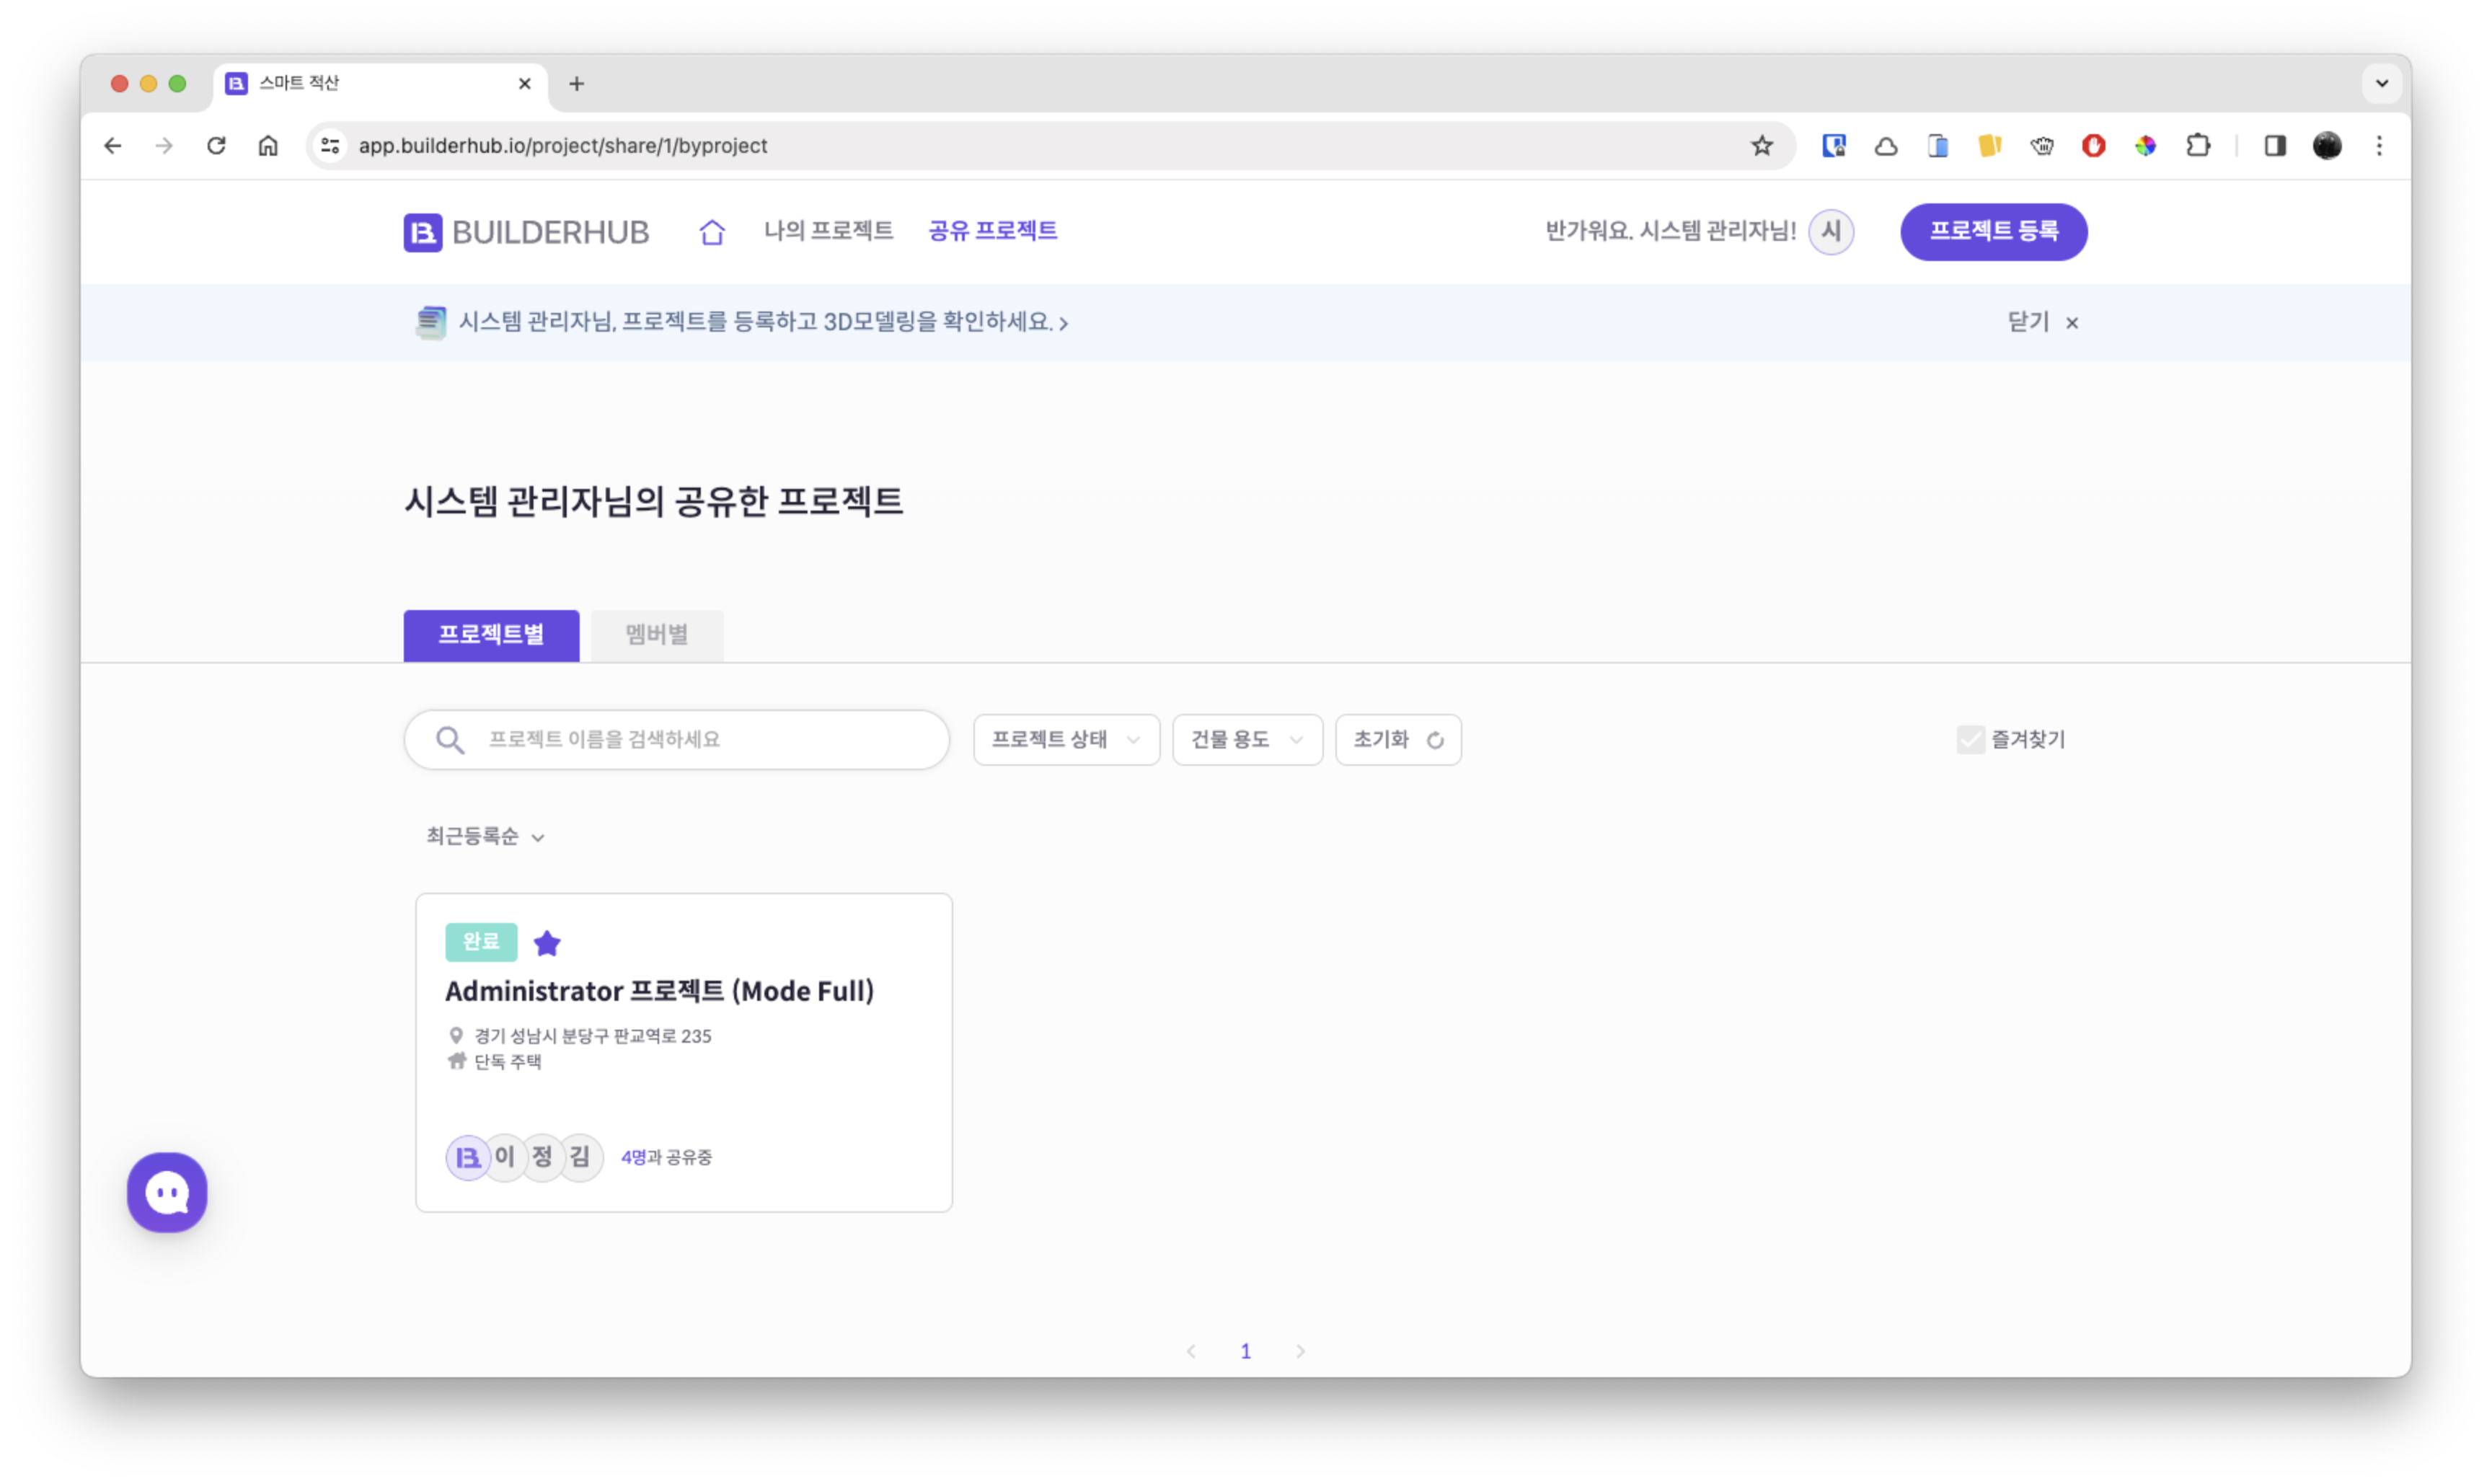
\includegraphics[width=0.35\textwidth]{images/builderhub-customer-project-3.png}
					            \caption*{Sharing project}
				            }\qquad
				            \parbox{0.35\textwidth}{
					            \centering
					            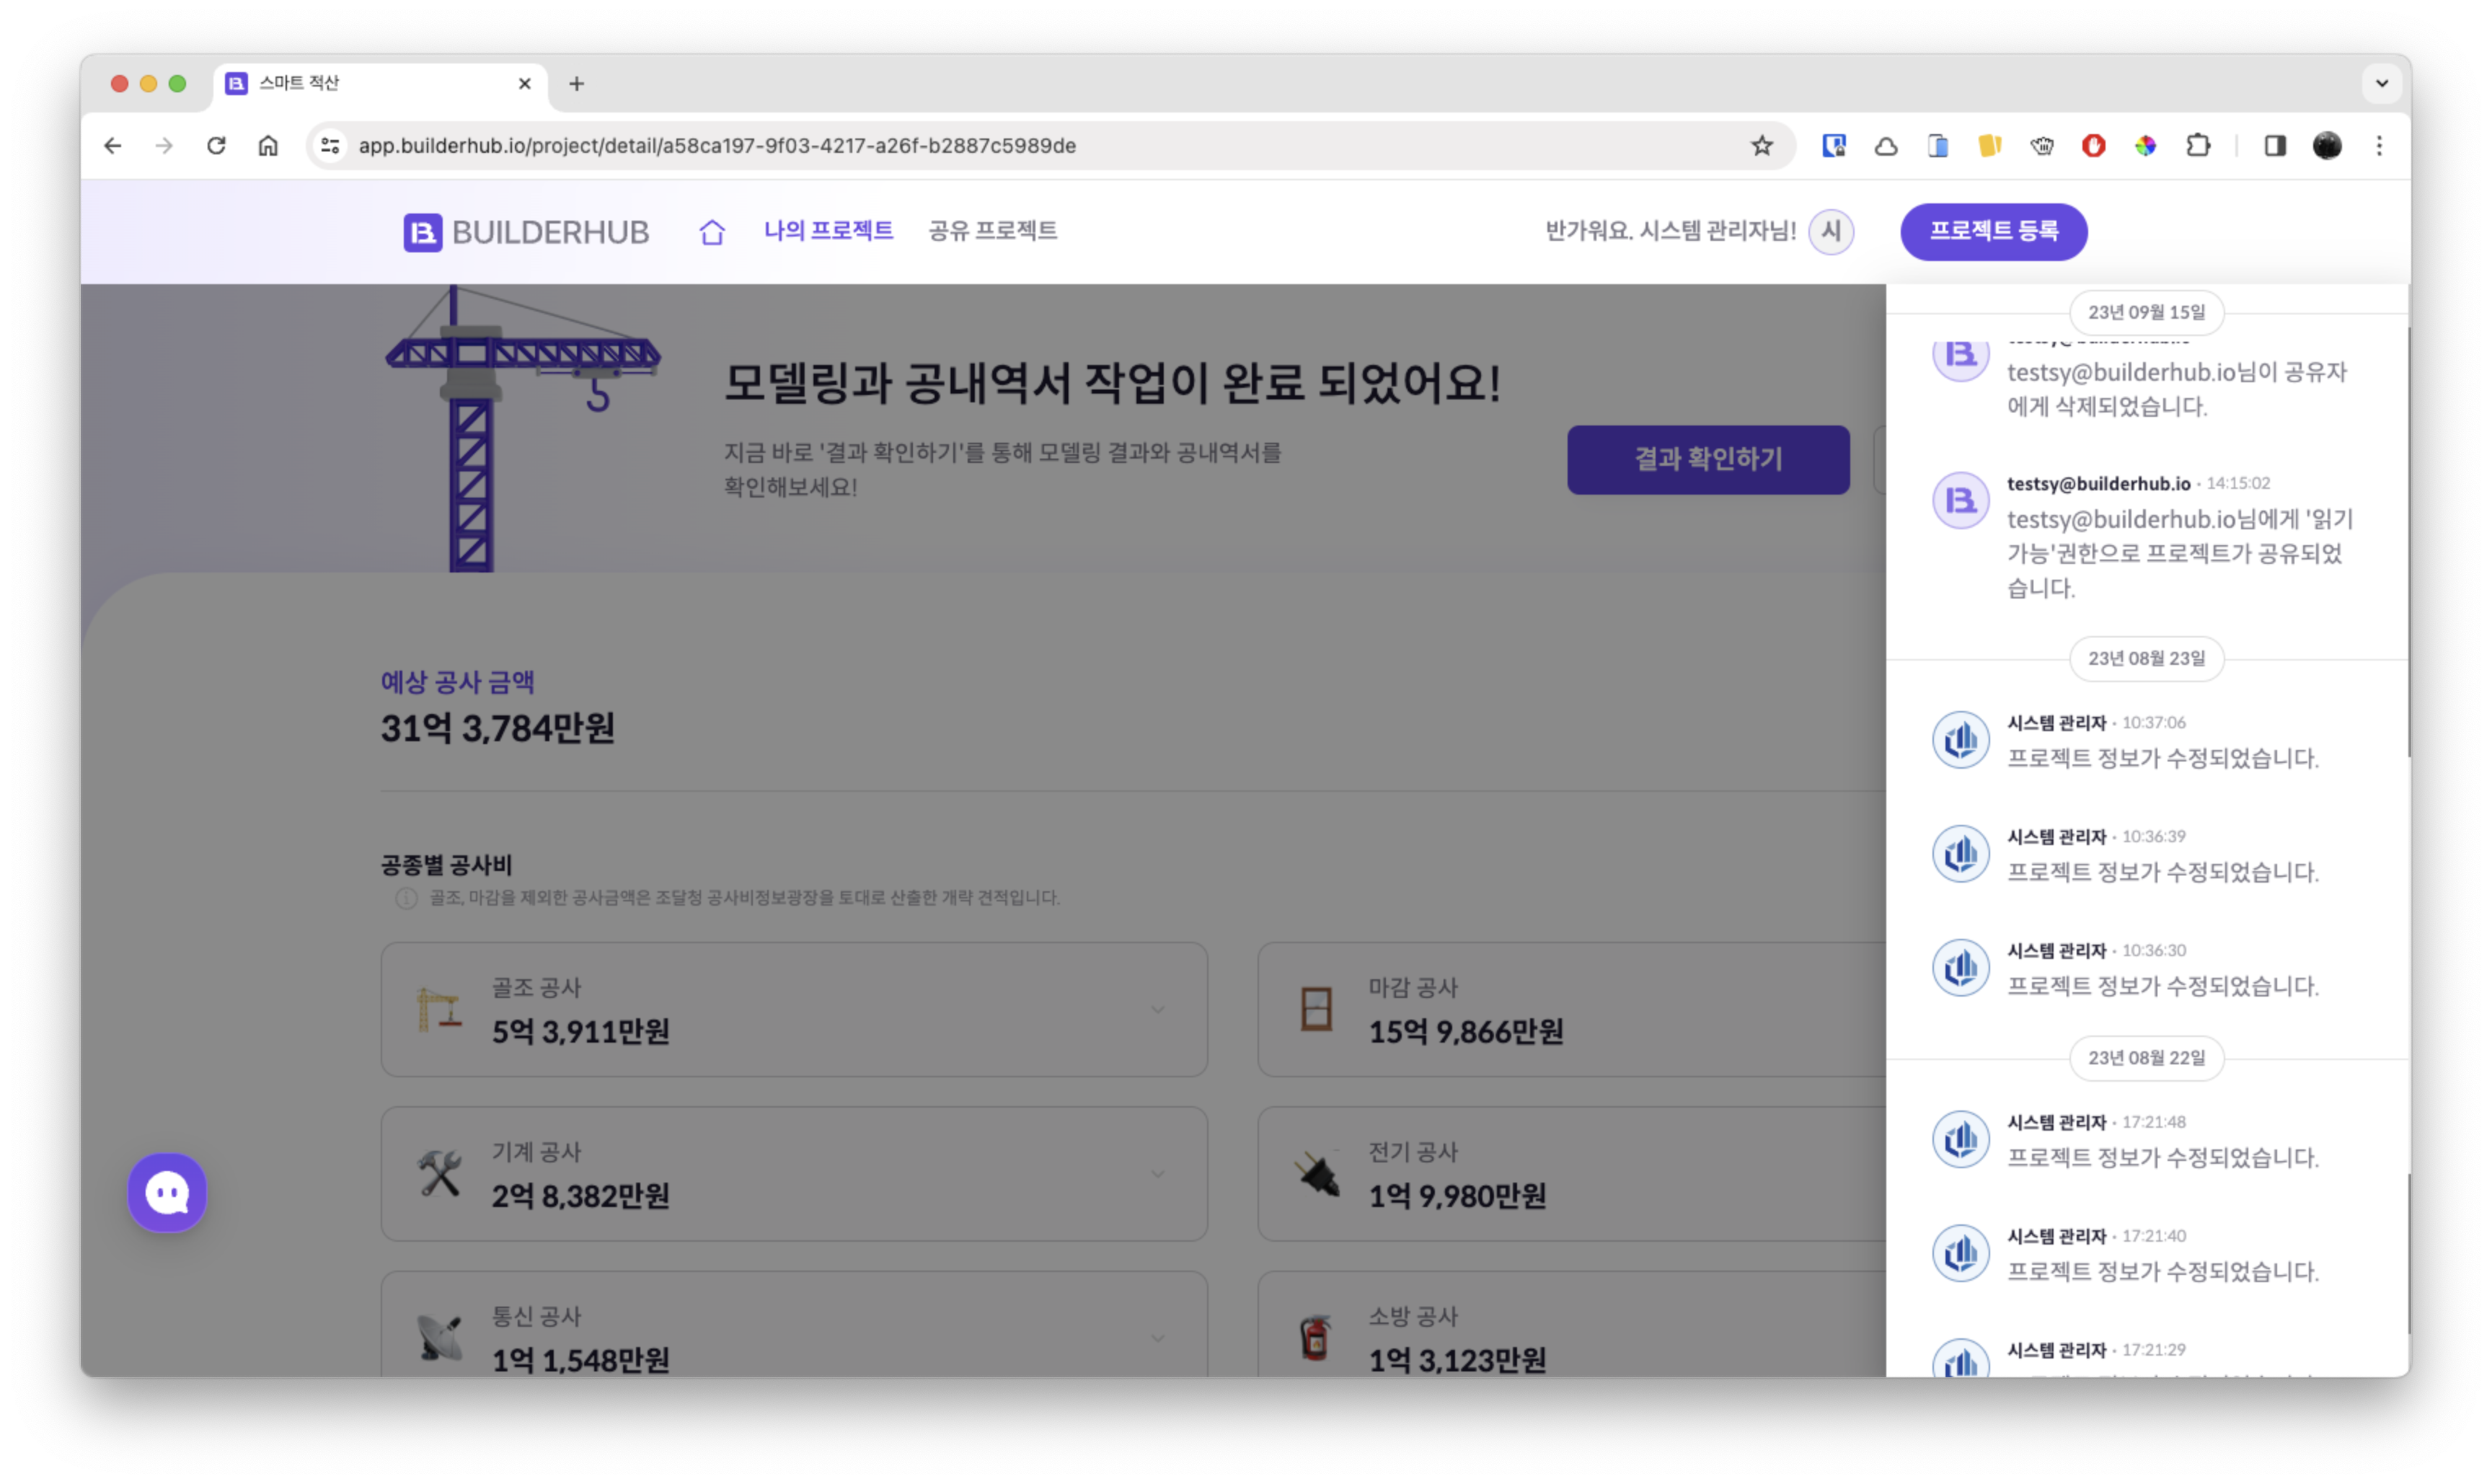
\includegraphics[width=0.35\textwidth]{images/builderhub-customer-project-4.png}
					            \caption*{Project history \& detail}
				            }
			            \end{fullwidth}
		            \end{figure}
		            \clearpage
		      \item \textbf{\href{https://curation.builderhub.io/project/tester}{큐레이션 서비스} 개발}
		            \begin{itemize}
			            \item BIM 모델 3D 뷰어: Three.js, Forge API, Zoom to Control, First-person View Control
			            \item 내역 필터 및 검색: Floor Filter, Material Filter, Table Filter, Search
			            \item 모델 툴 개발: Section View, Screenshot, Measurement
			            \item 자재 변경, 도면 뷰어
			            \item 공정 시뮬레이션, 공정표 제공: Gantt Chart, Work simulation (on developing)
		            \end{itemize}
		            \begin{figure}[!ht]
			            \begin{fullwidth}
				            \parbox{0.35\textwidth}{
					            \centering
					            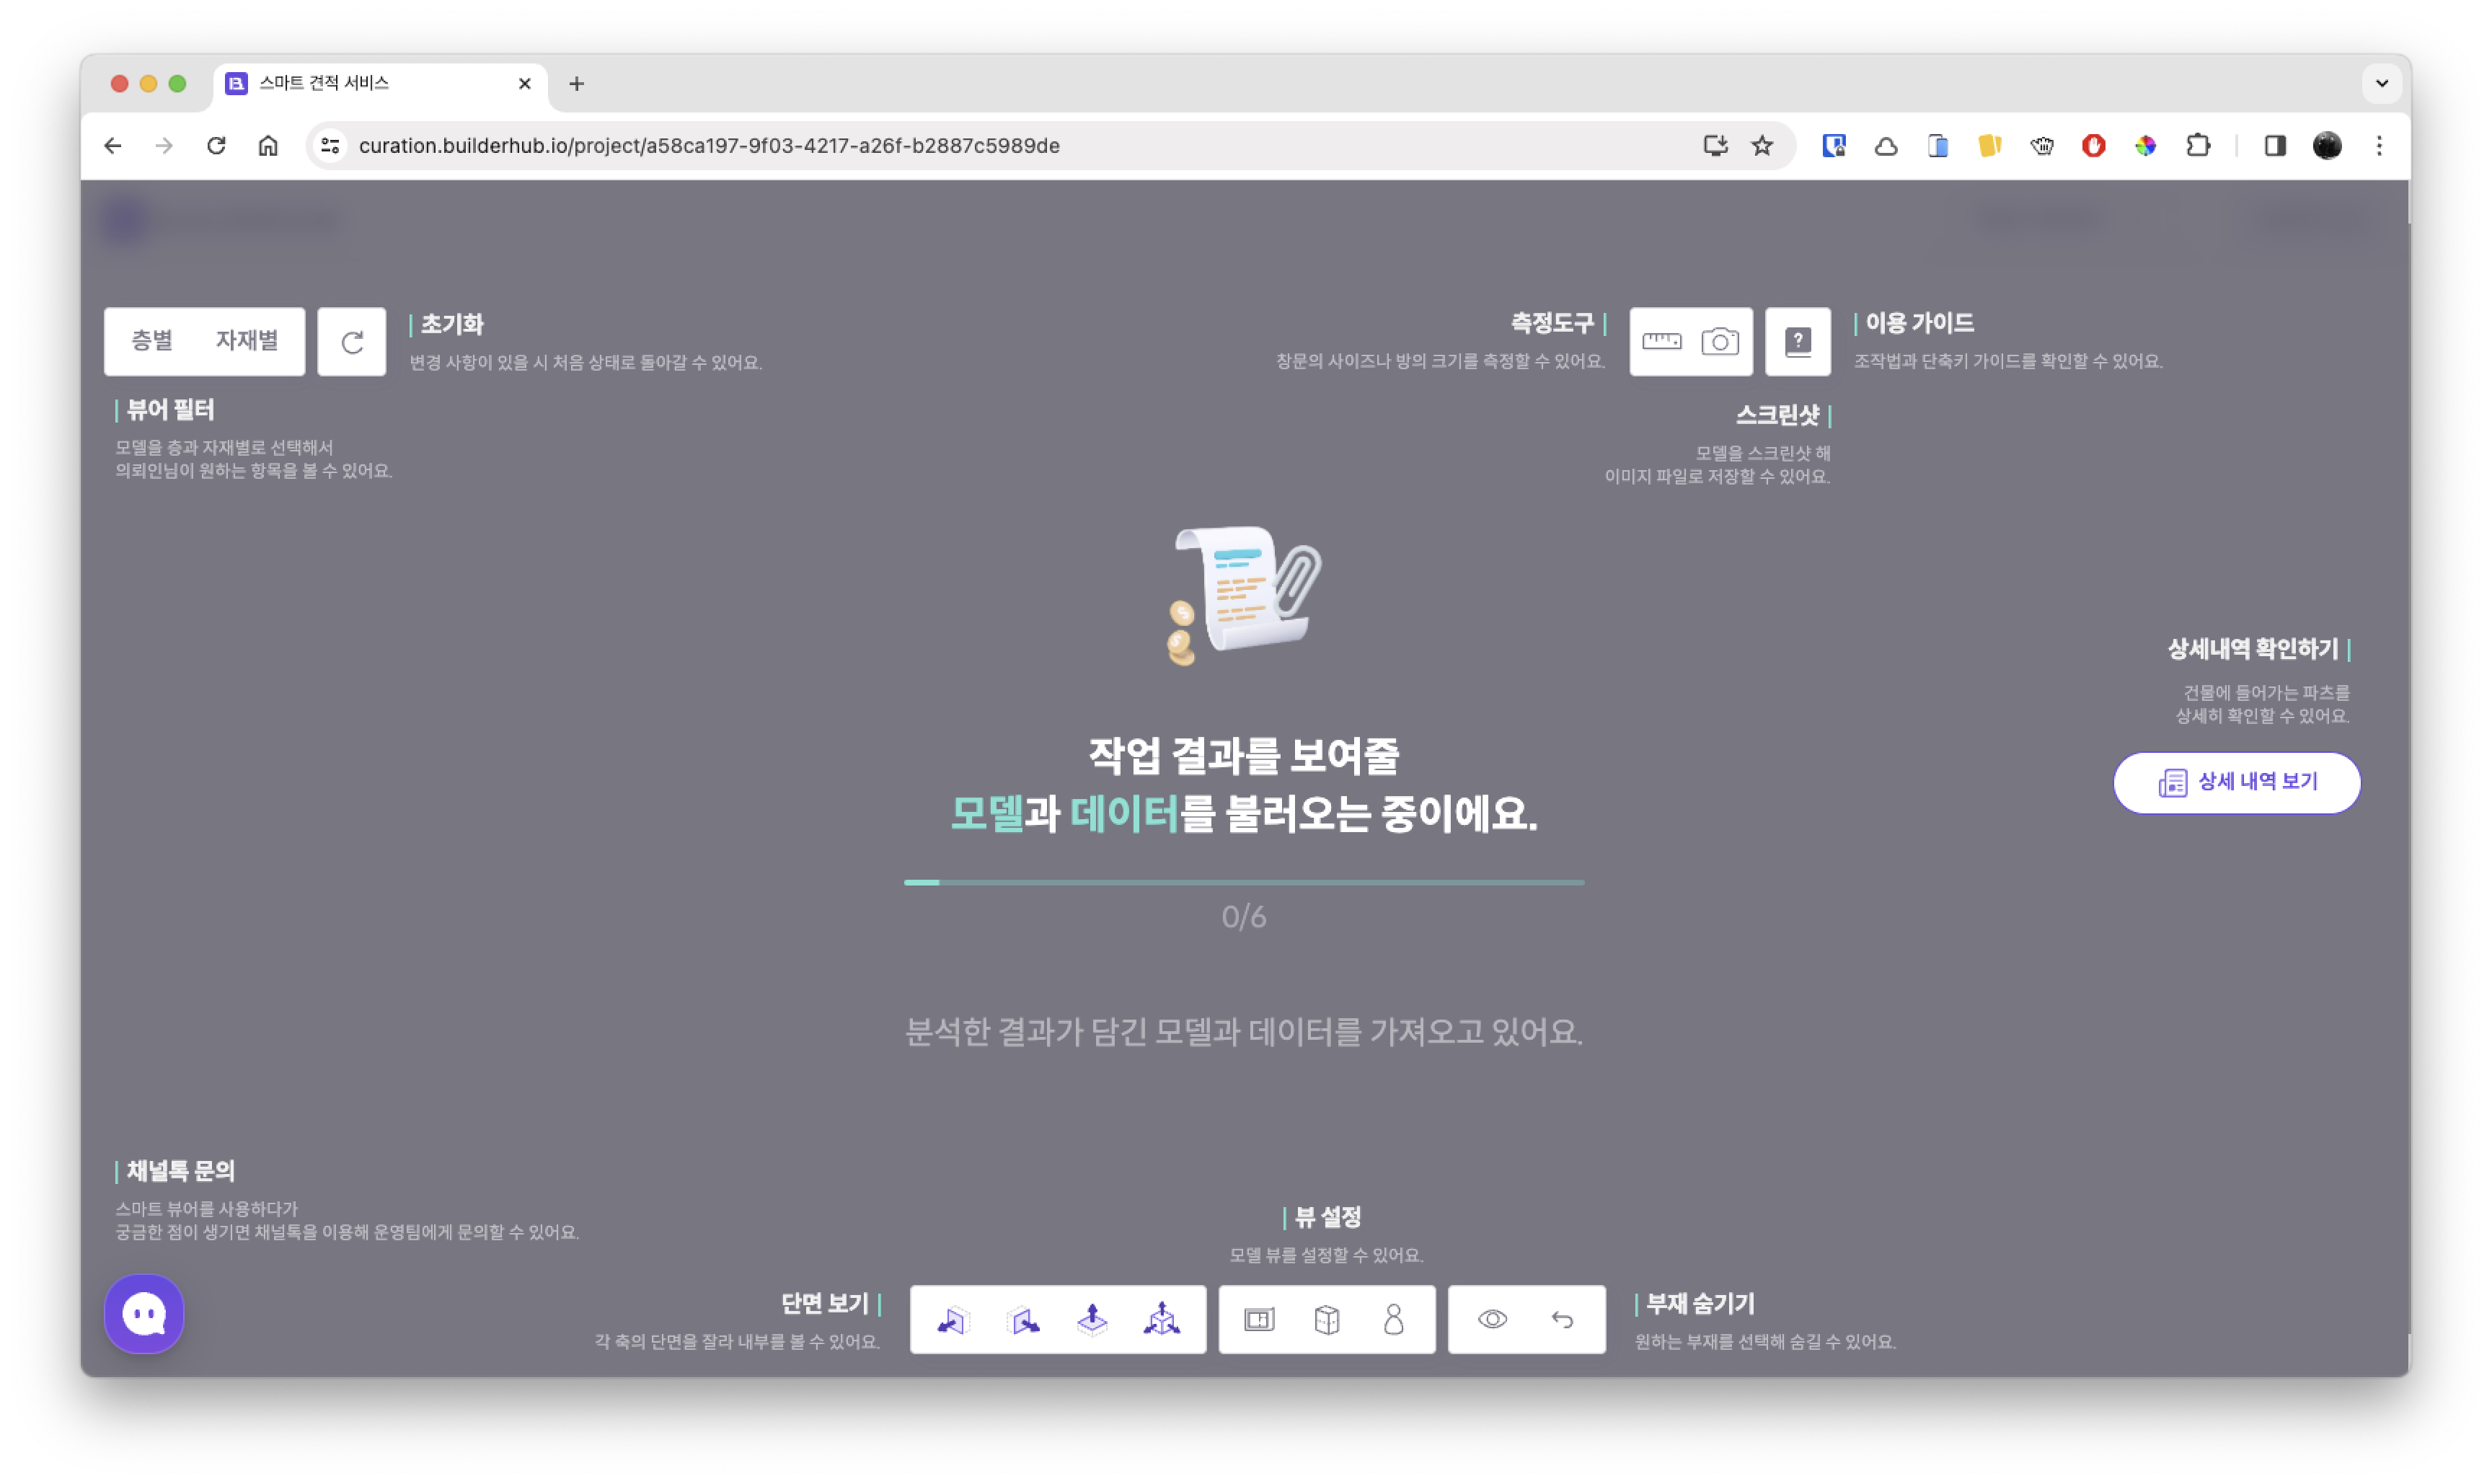
\includegraphics[width=0.35\textwidth]{images/builderhub-curation-loader-1.png}
					            \caption*{Loader}
				            }\qquad
				            \parbox{0.35\textwidth}{
					            \centering
					            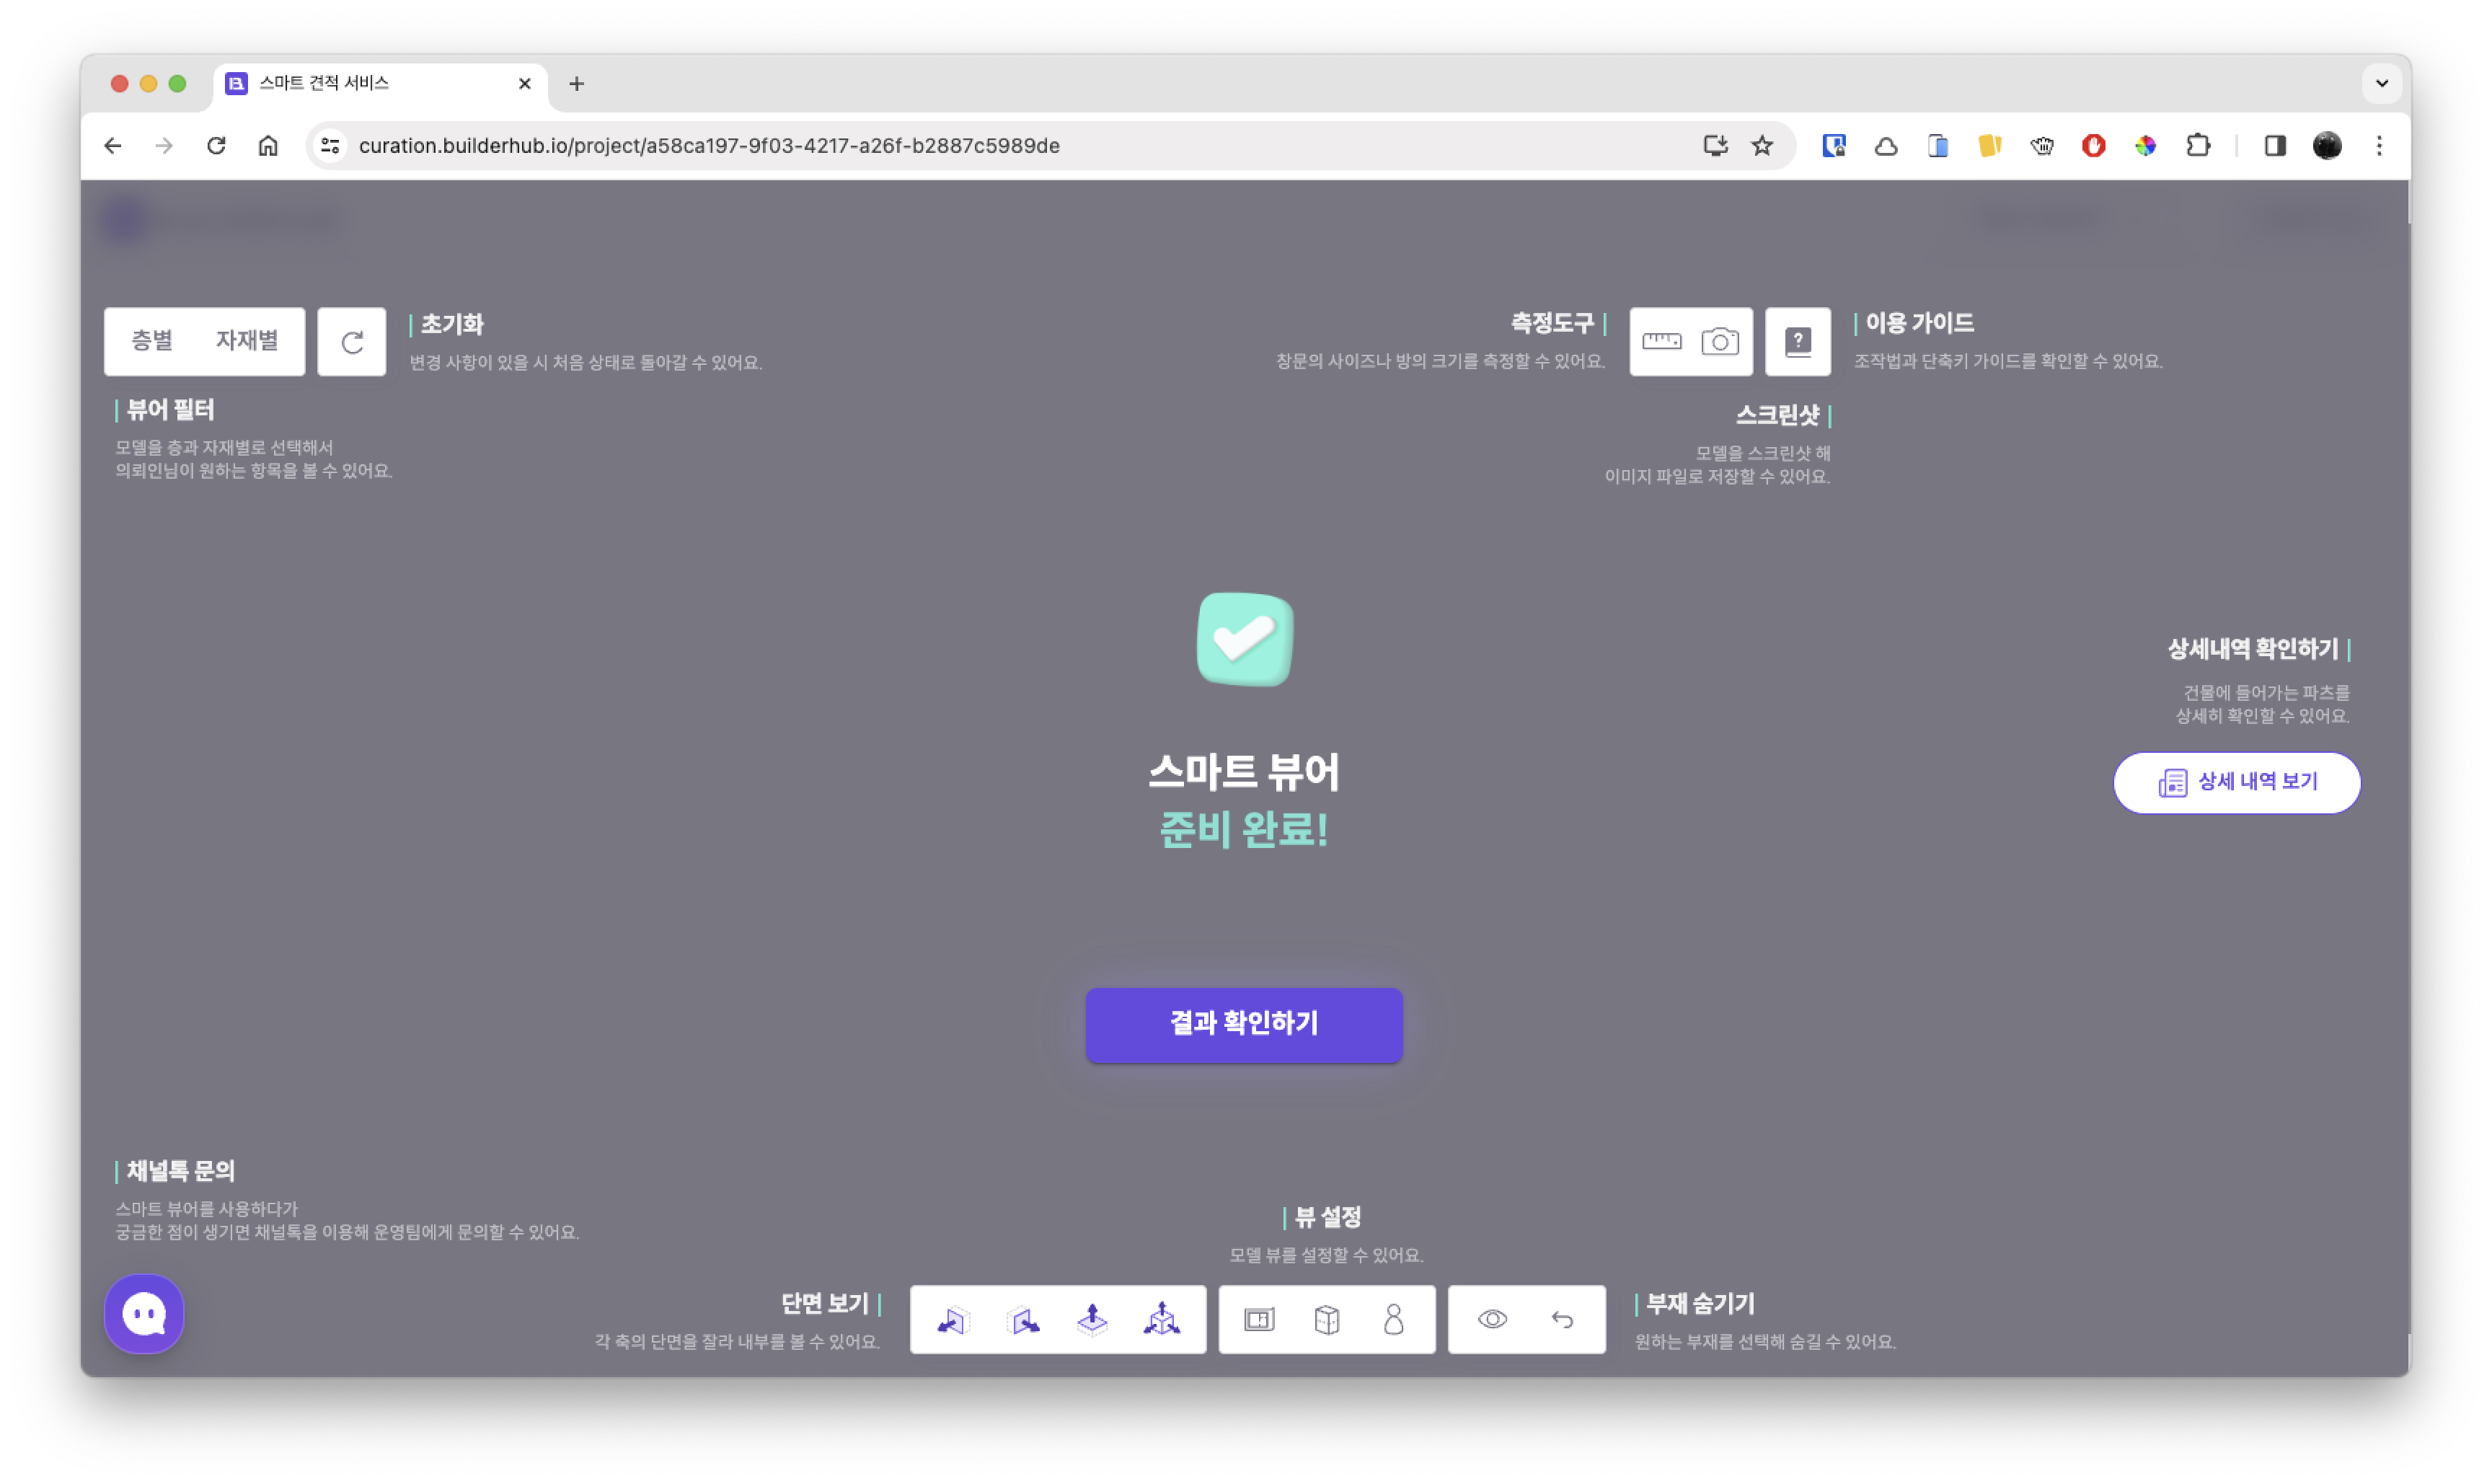
\includegraphics[width=0.35\textwidth]{images/builderhub-curation-loader-2.png}
					            \caption*{Loading done}
				            }\qquad
				            \parbox{0.35\textwidth}{
					            \centering
					            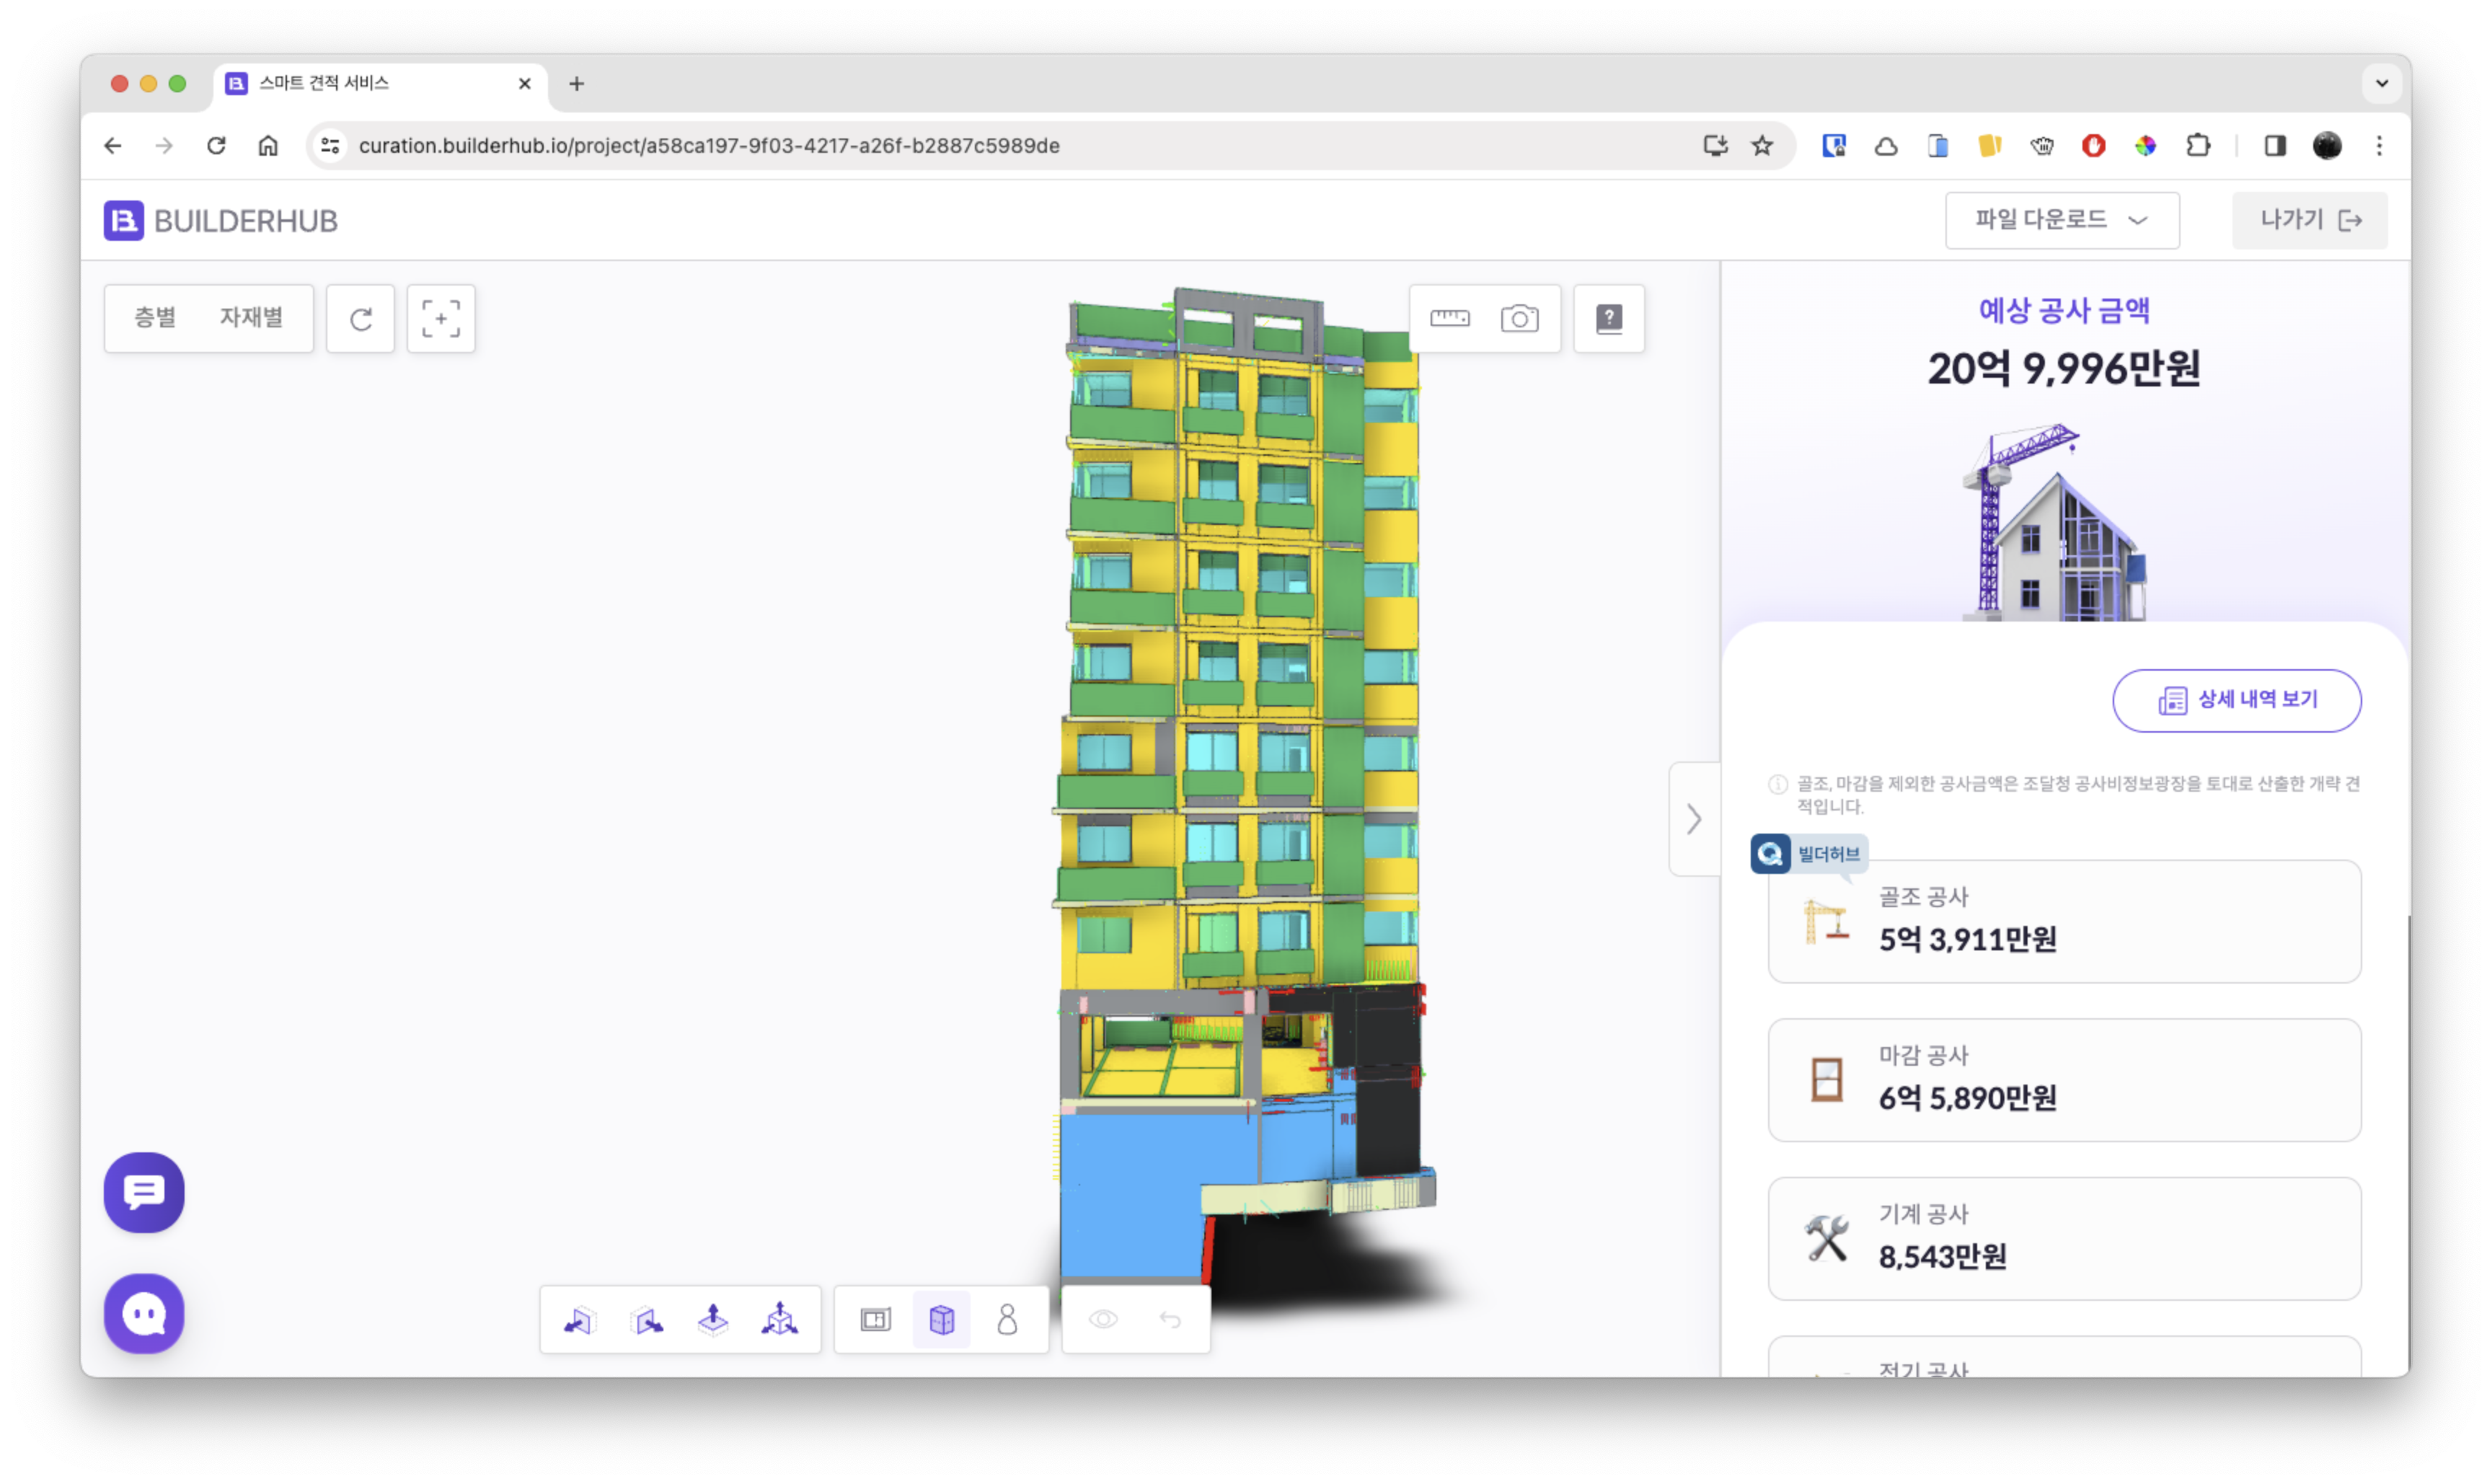
\includegraphics[width=0.35\textwidth]{images/builderhub-curation-main.png}
					            \caption*{Main view}
				            }\qquad
				            \parbox{0.35\textwidth}{
					            \centering
					            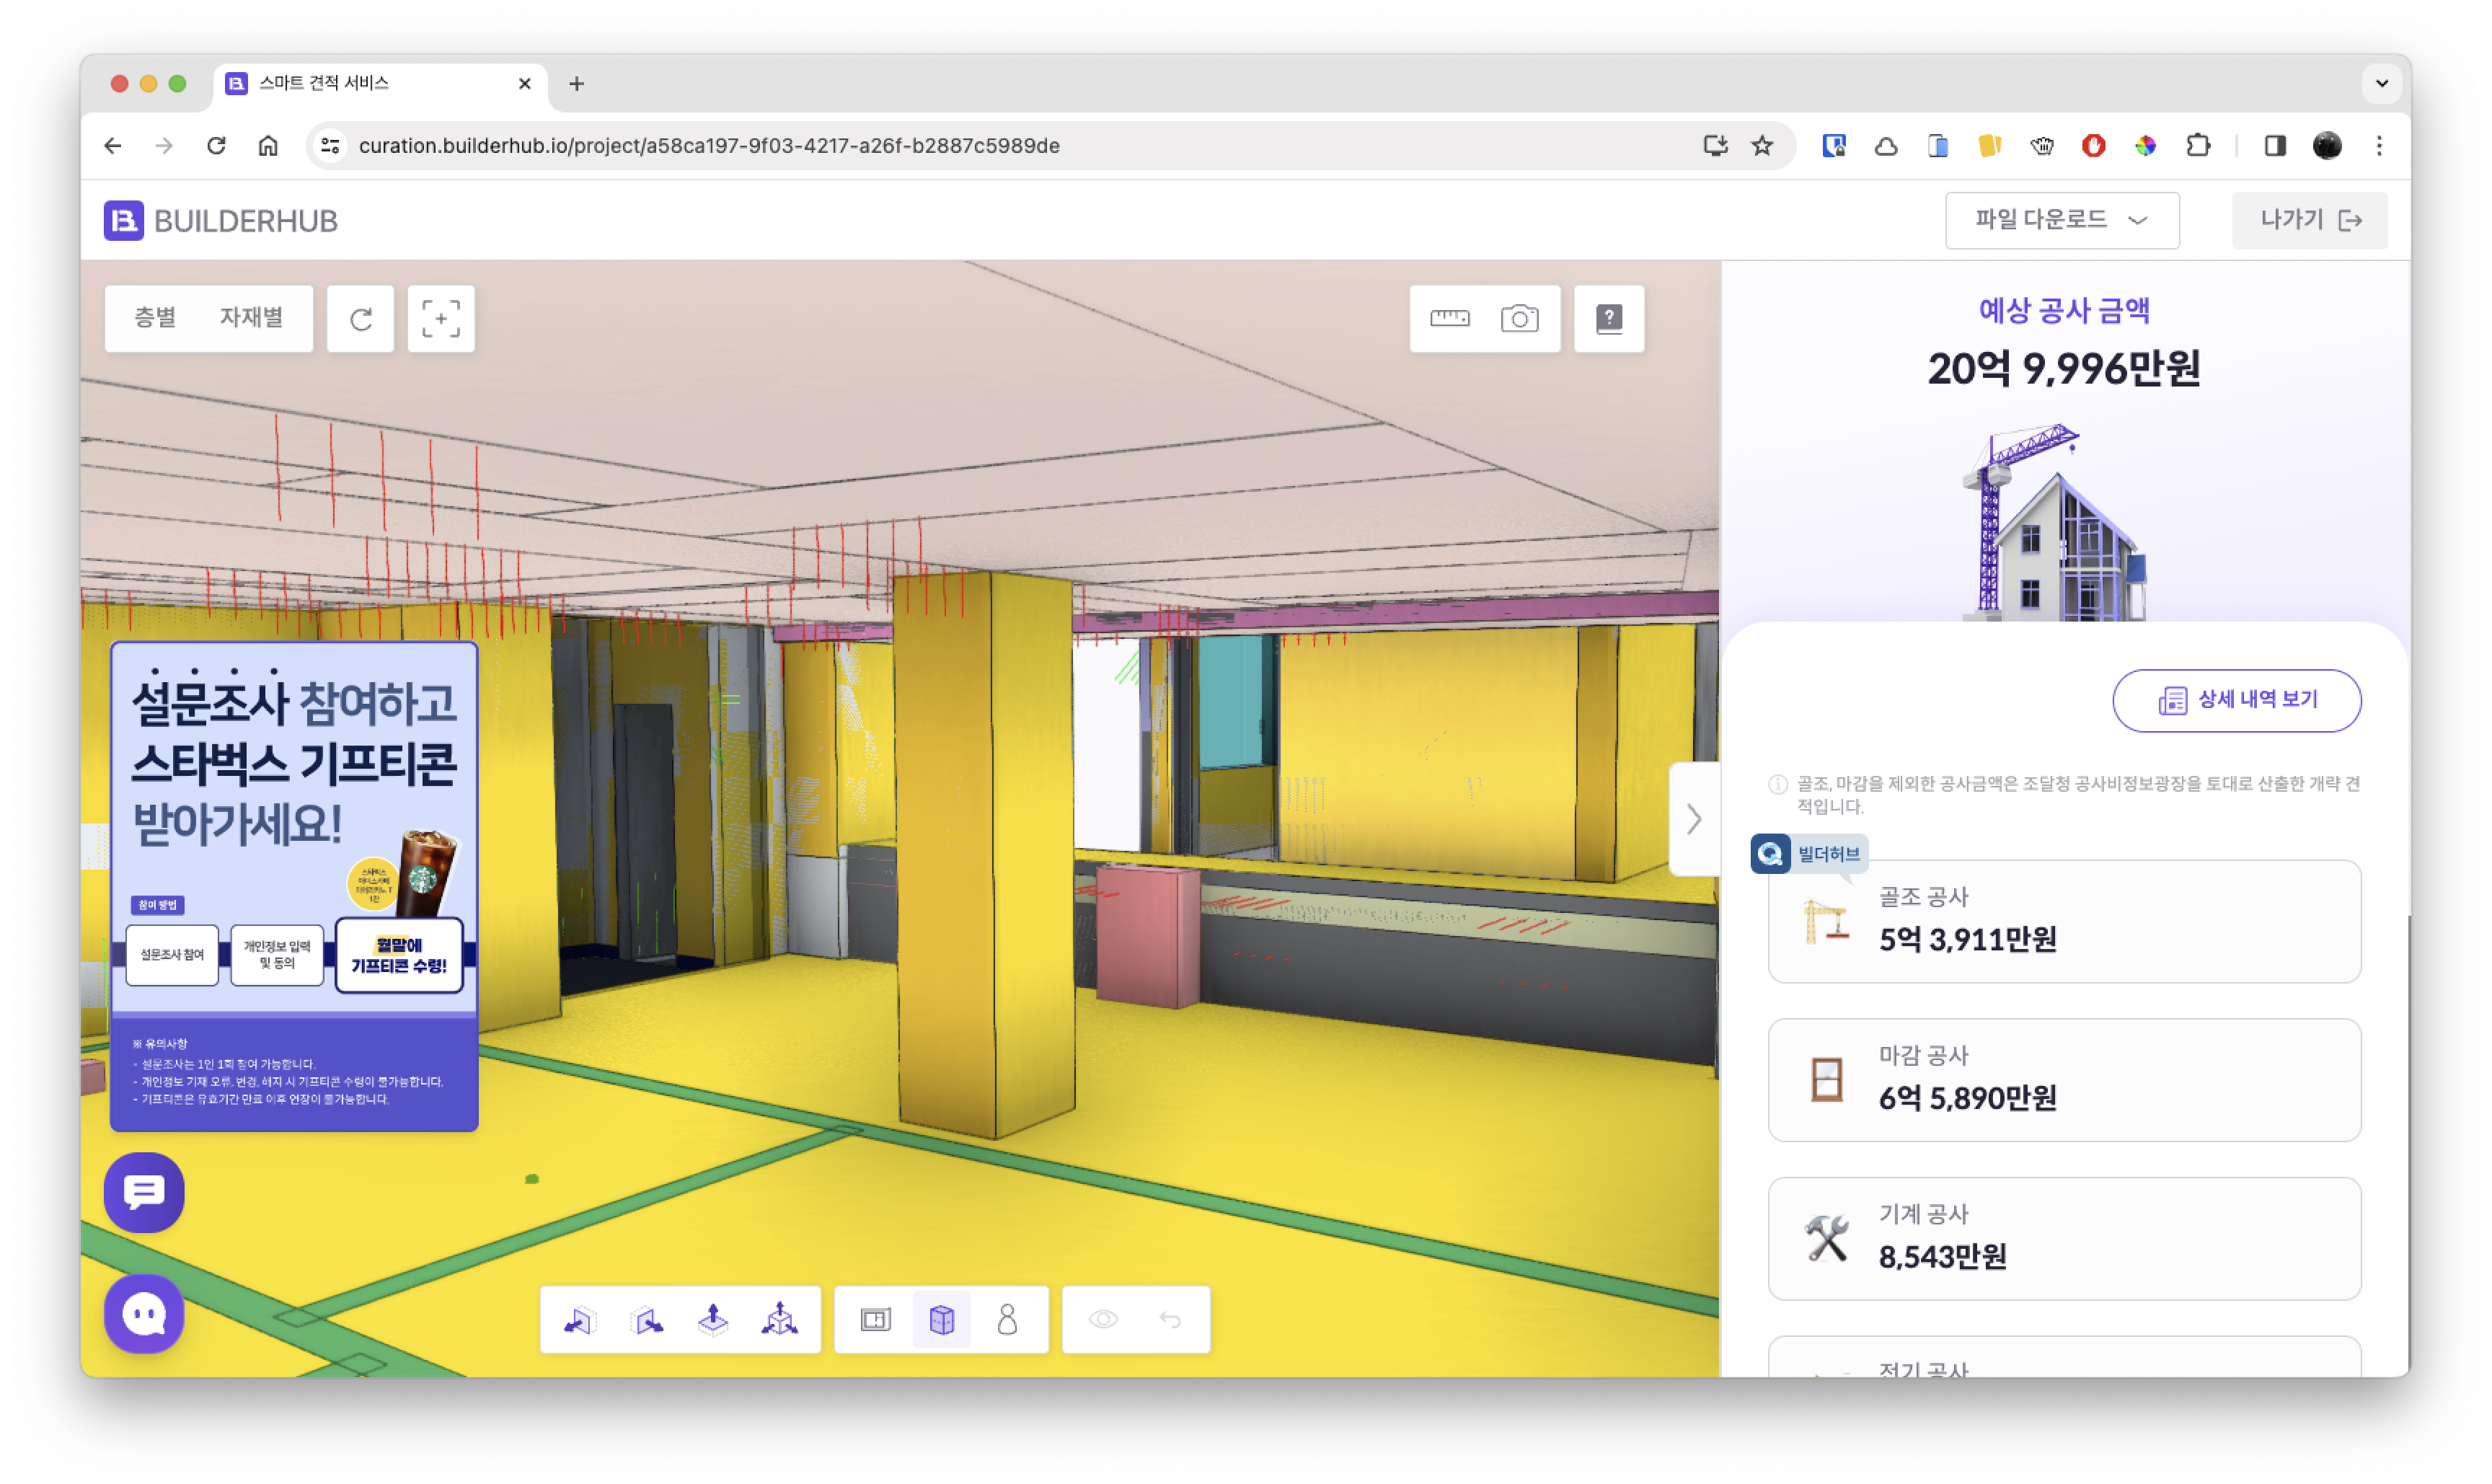
\includegraphics[width=0.35\textwidth]{images/builderhub-curation-control.png}
					            \caption*{Control orbit}
				            }
				            \parbox{0.35\textwidth}{
					            \centering
					            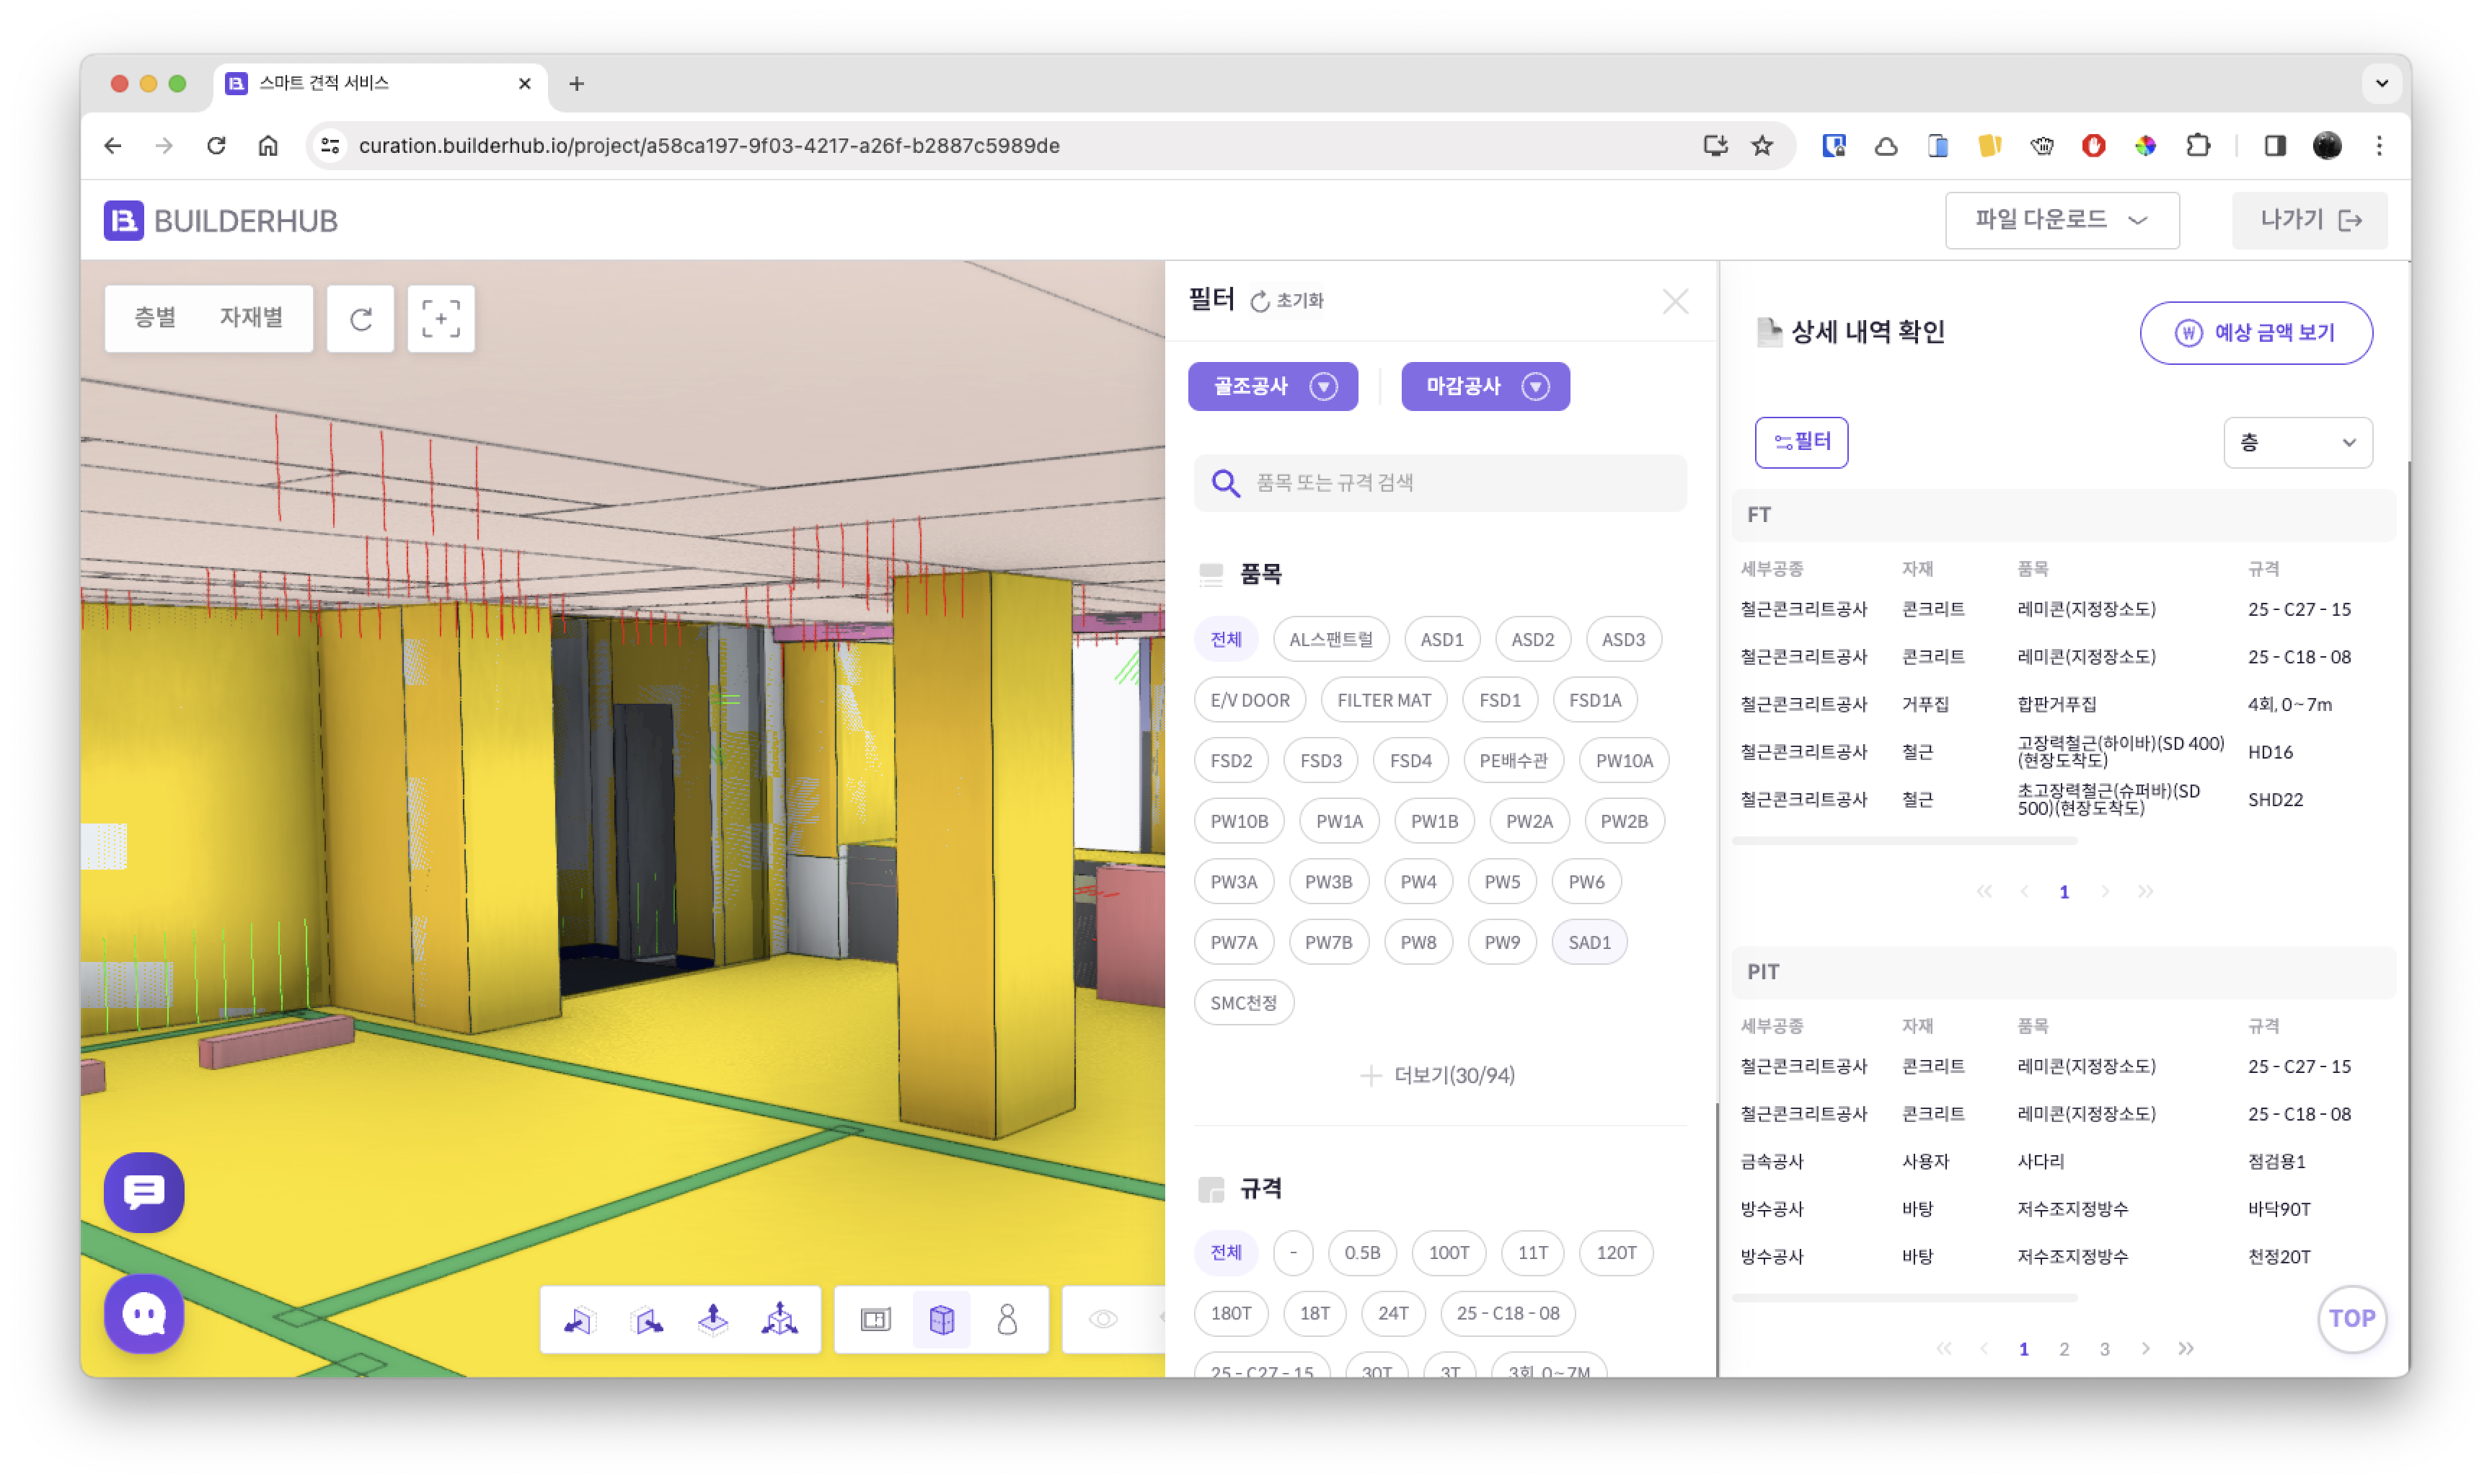
\includegraphics[width=0.35\textwidth]{images/builderhub-curation-filter.png}
					            \caption*{Filtering}
				            }\qquad
				            \parbox{0.35\textwidth}{
					            \centering
					            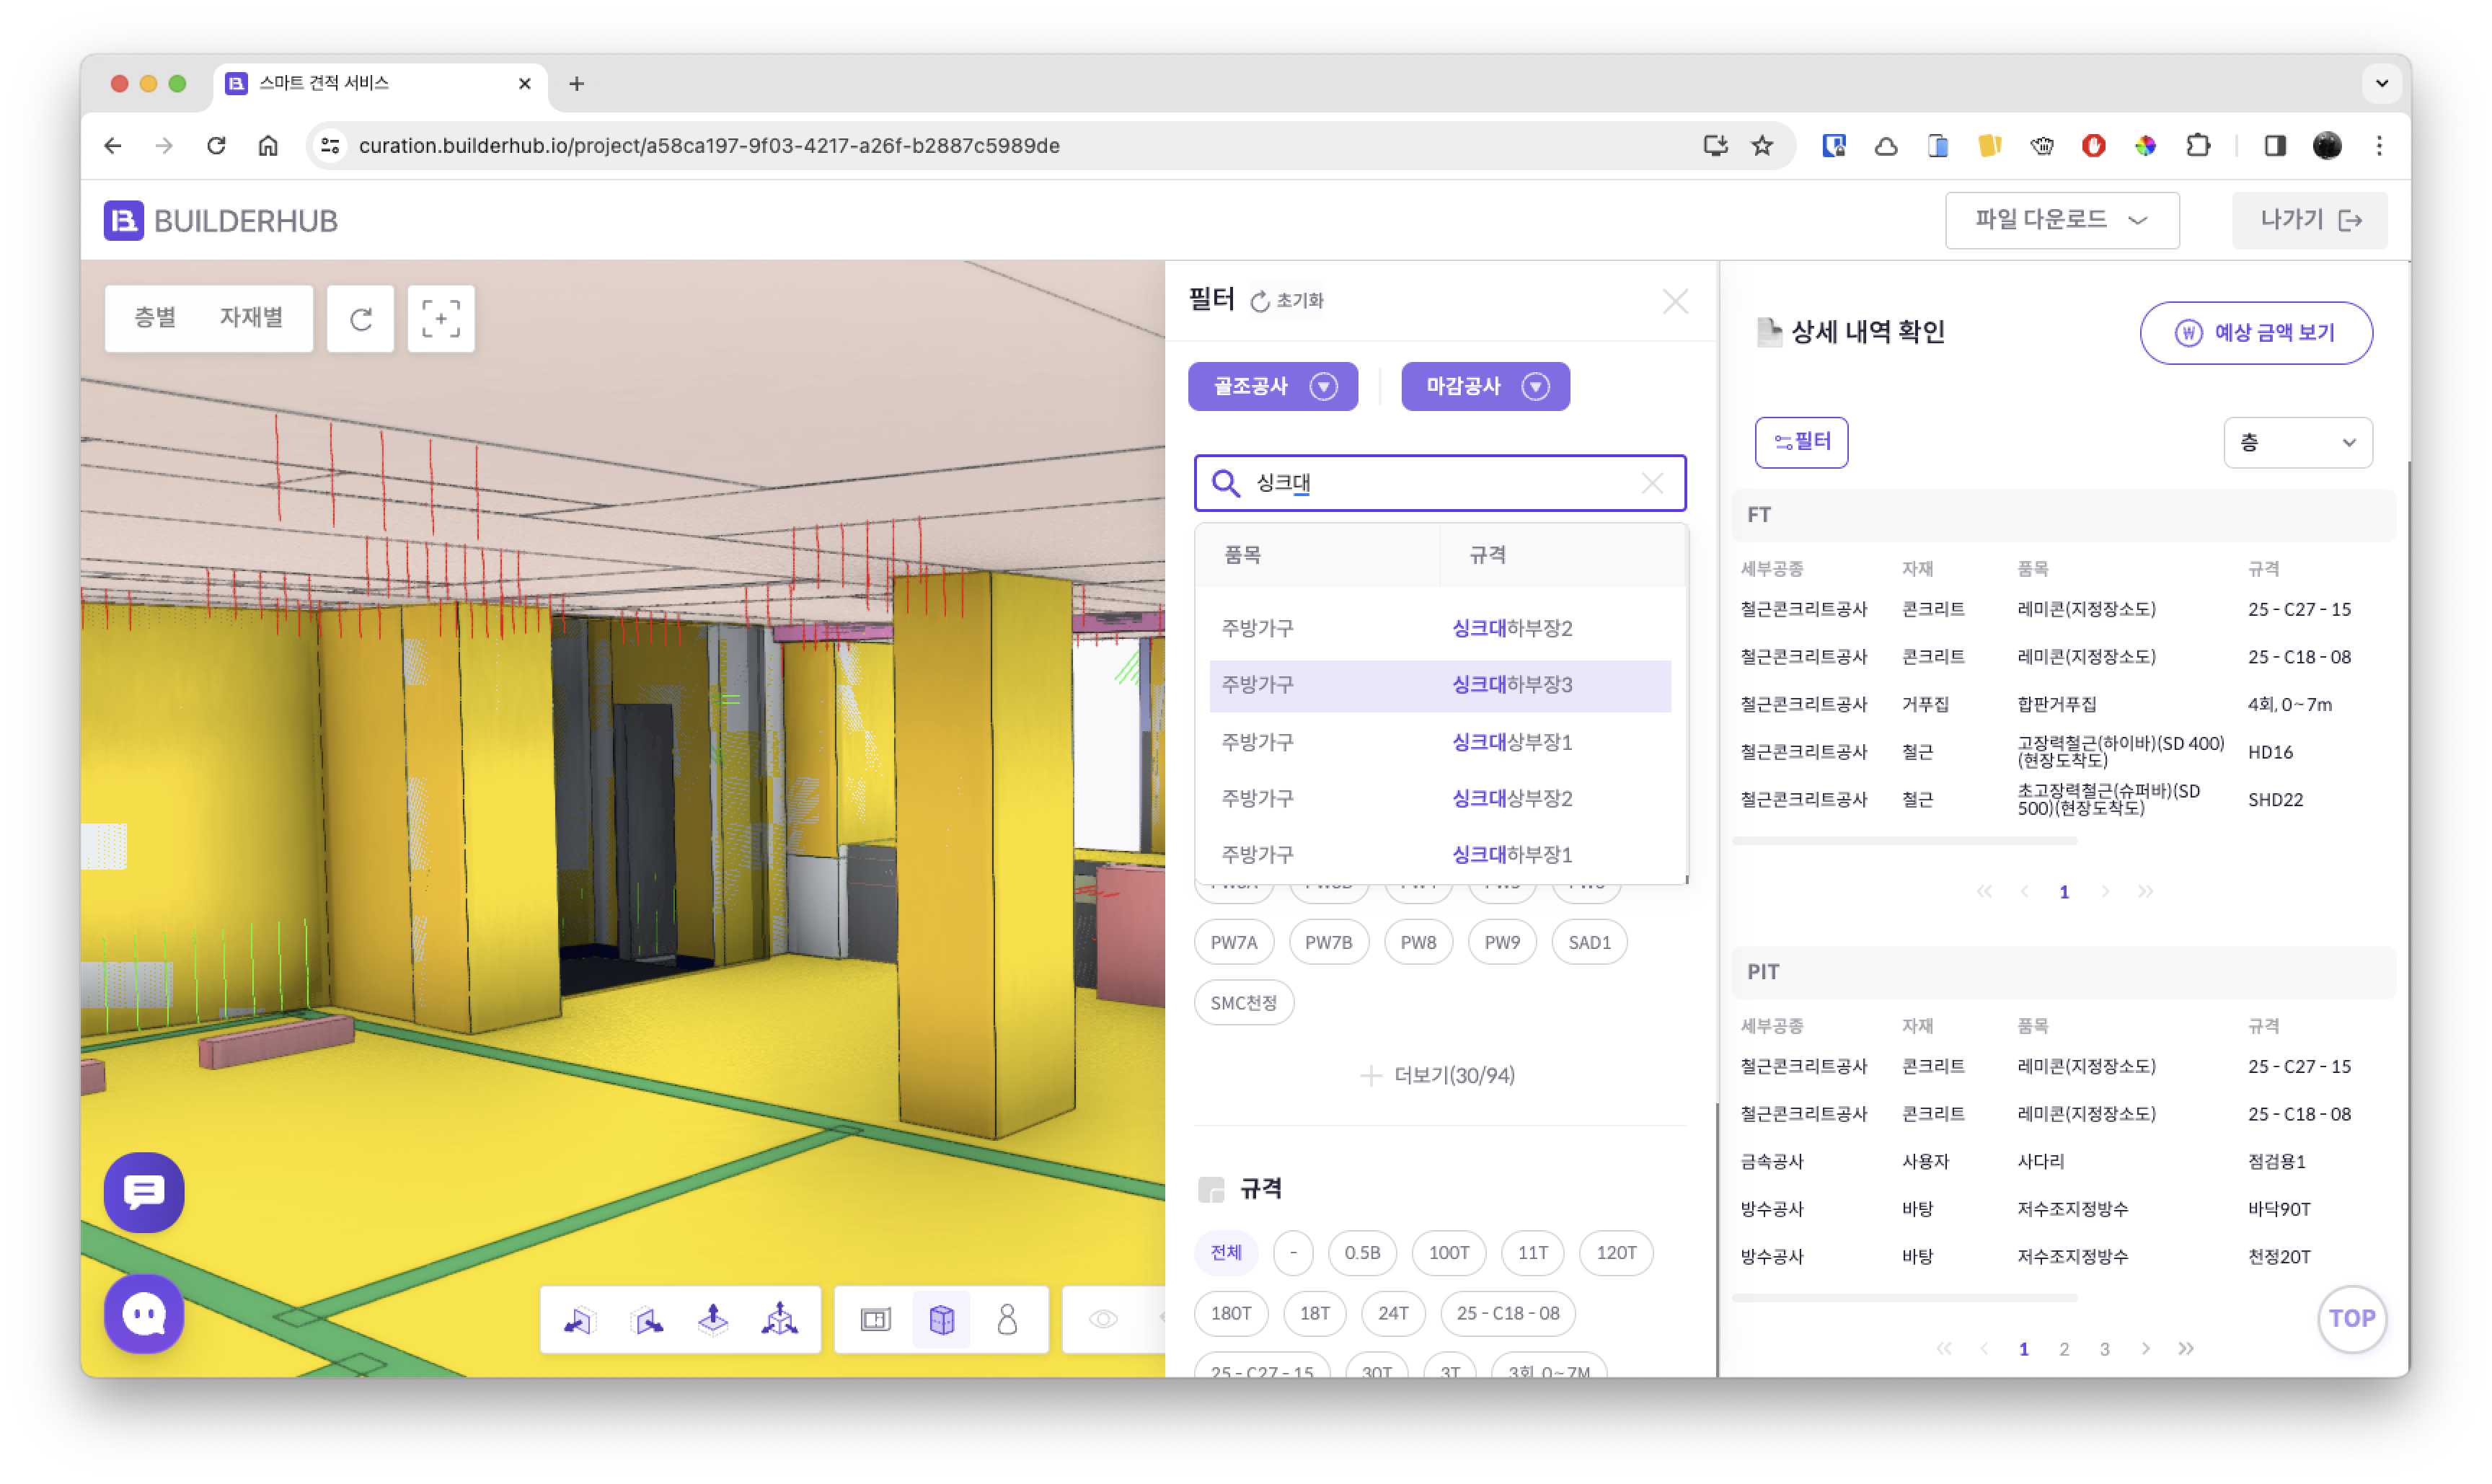
\includegraphics[width=0.35\textwidth]{images/builderhub-curation-filter-search.png}
					            \caption*{Search}
				            }\qquad
				            \parbox{0.35\textwidth}{
					            \centering
					            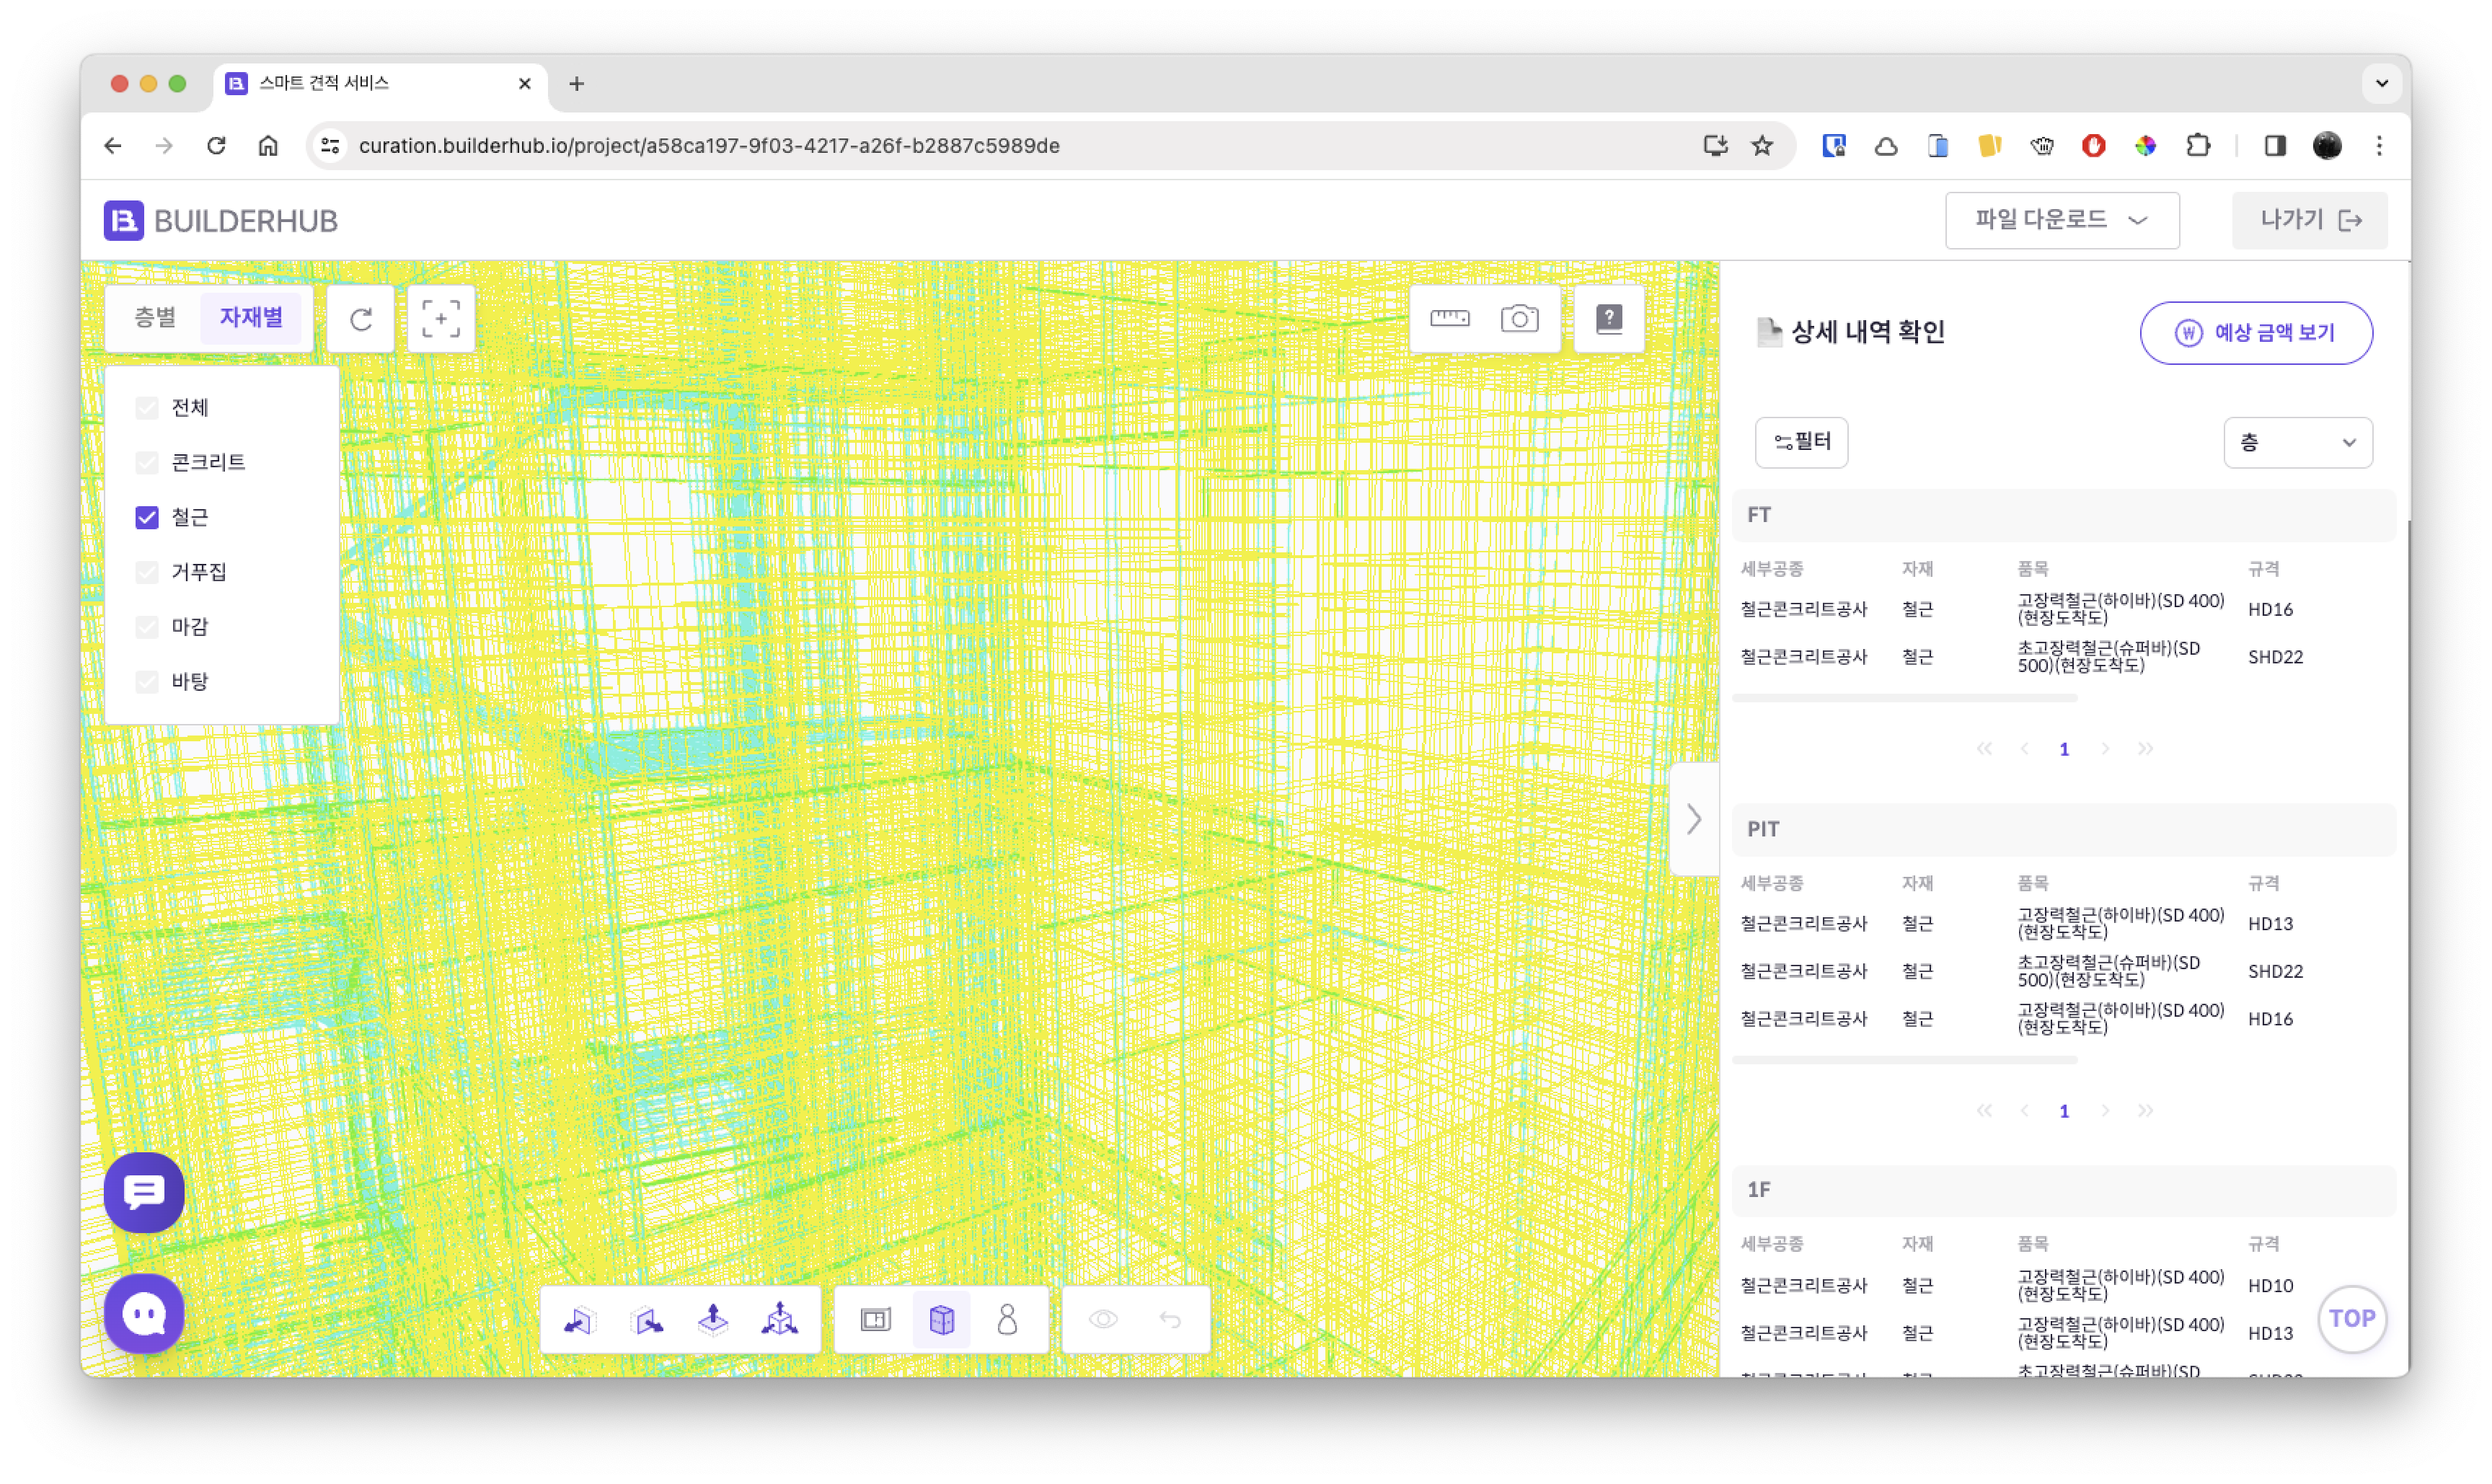
\includegraphics[width=0.35\textwidth]{images/builderhub-curation-filter-material.png}
					            \caption*{Material filter}
				            }\qquad
				            \parbox{0.35\textwidth}{
					            \centering
					            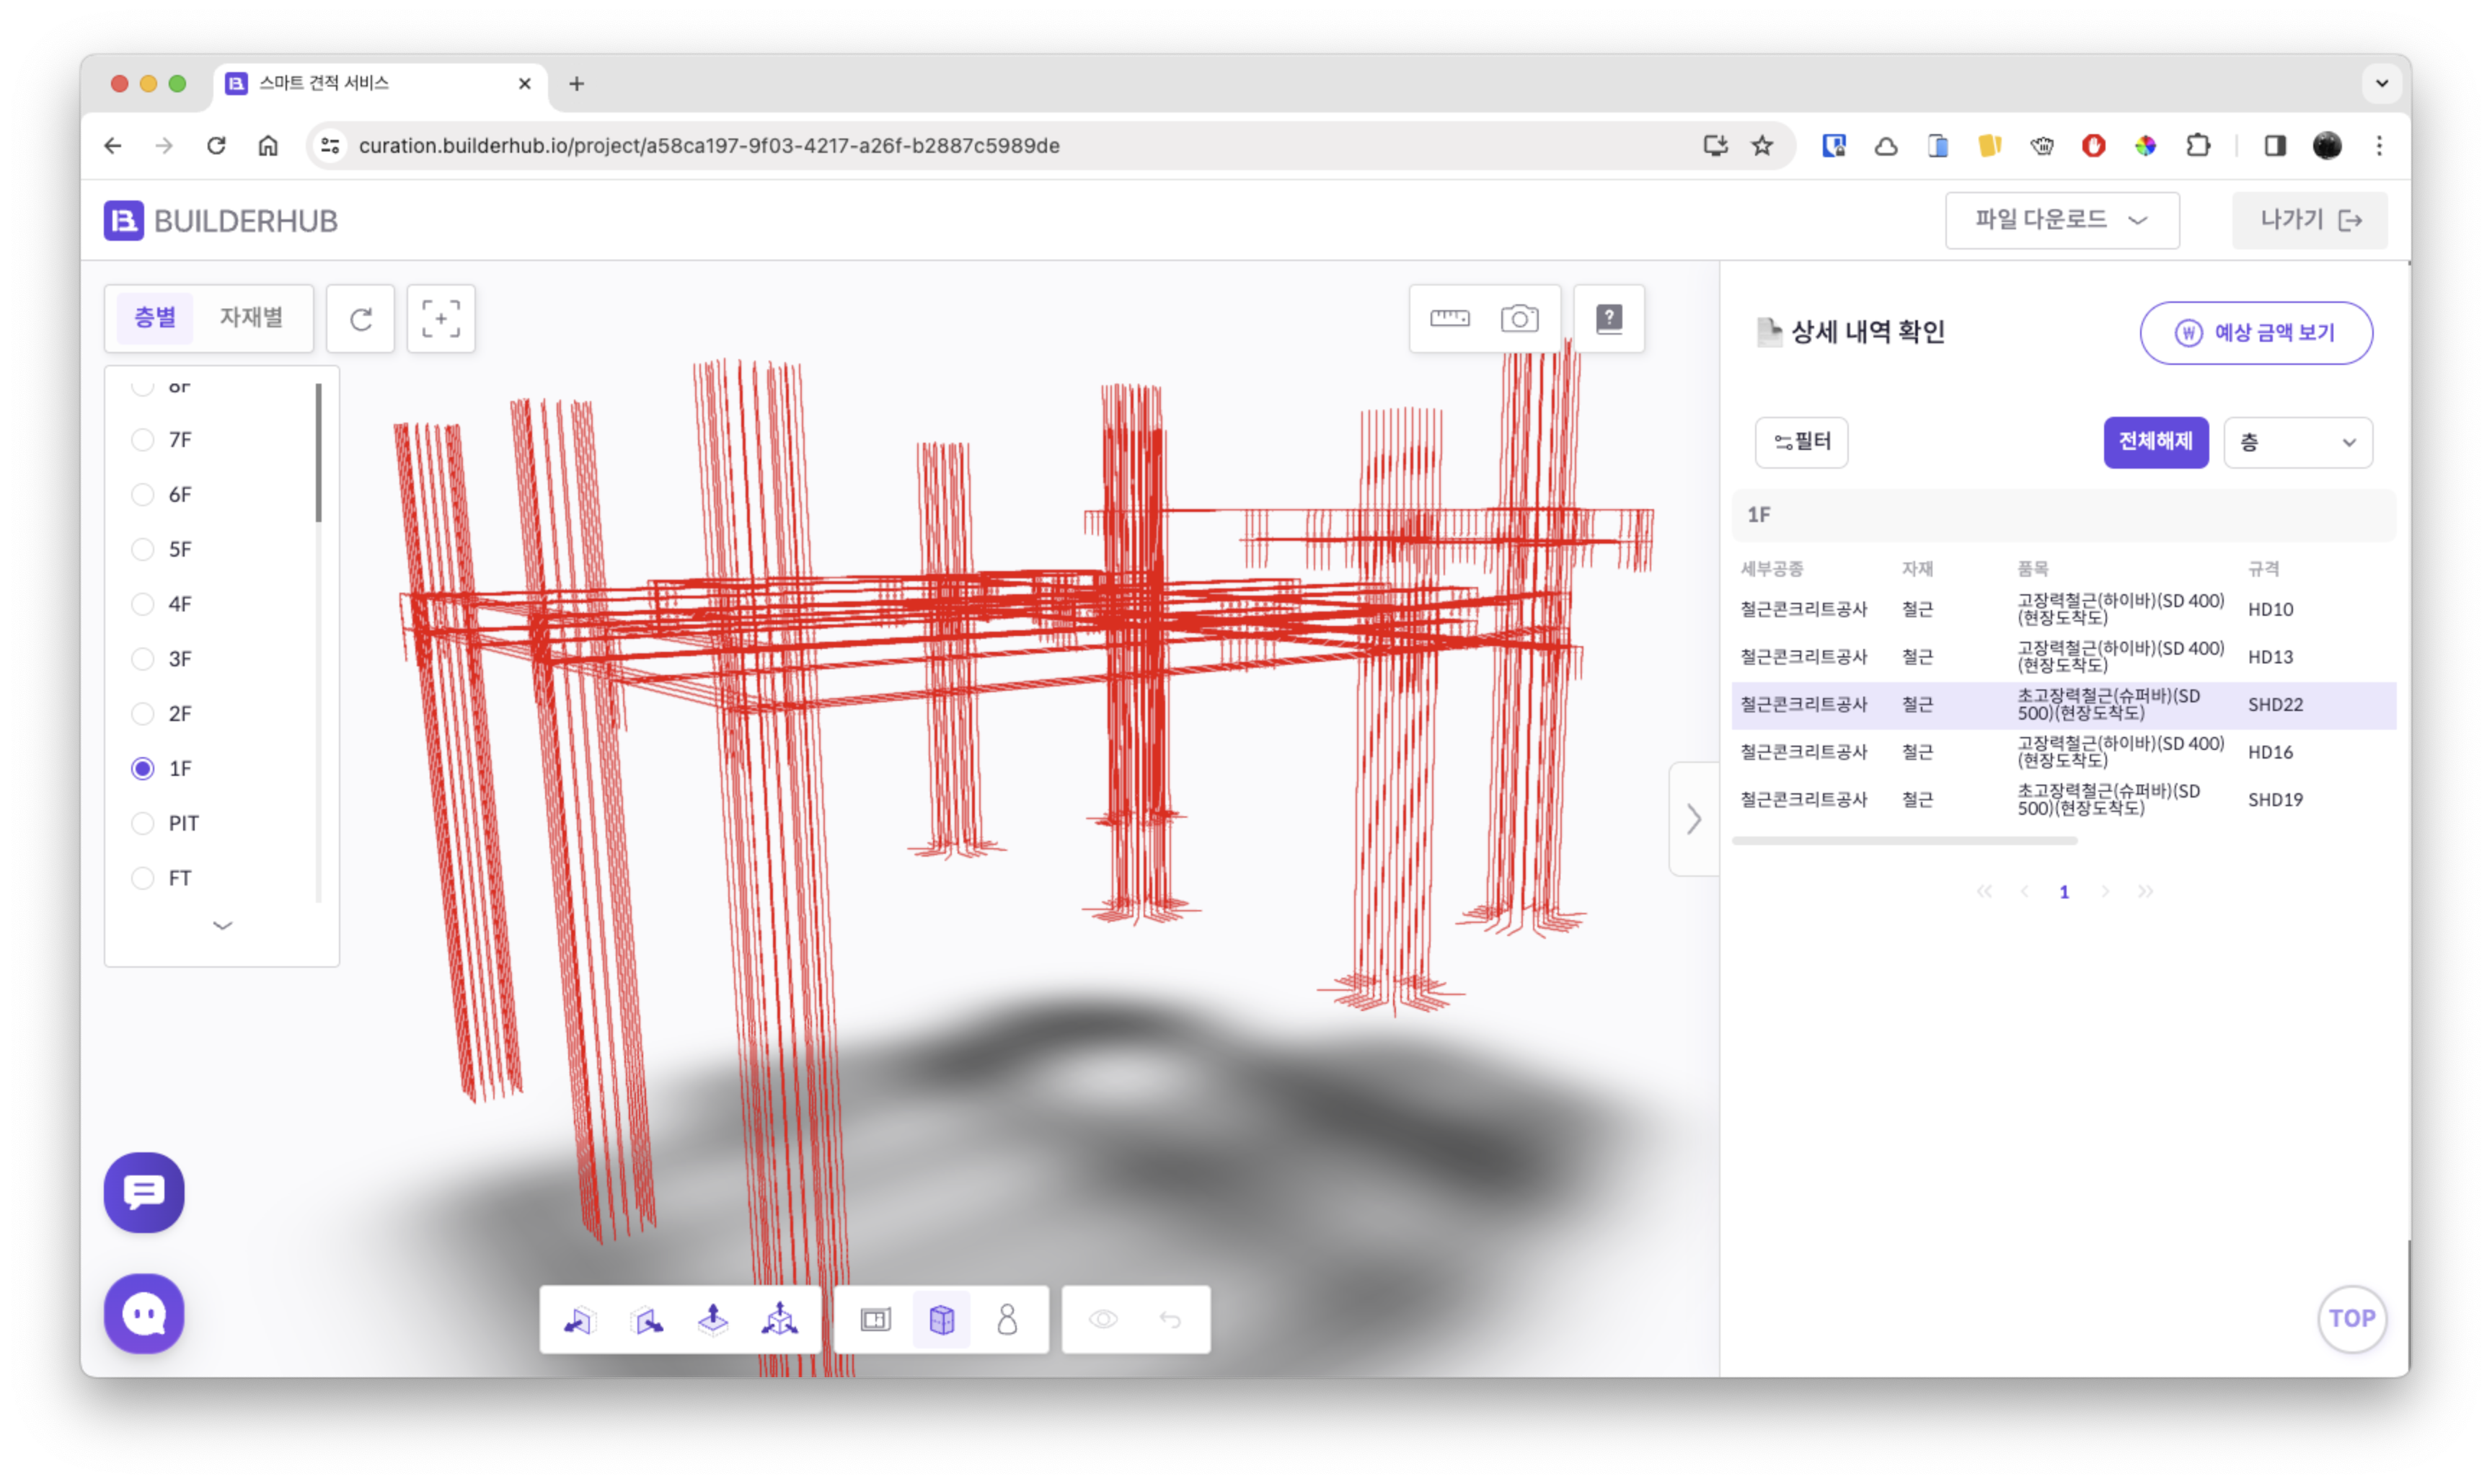
\includegraphics[width=0.35\textwidth]{images/builderhub-curation-filter-table.png}
					            \caption*{Table filter}
				            }
				            \parbox{0.35\textwidth}{
					            \centering
					            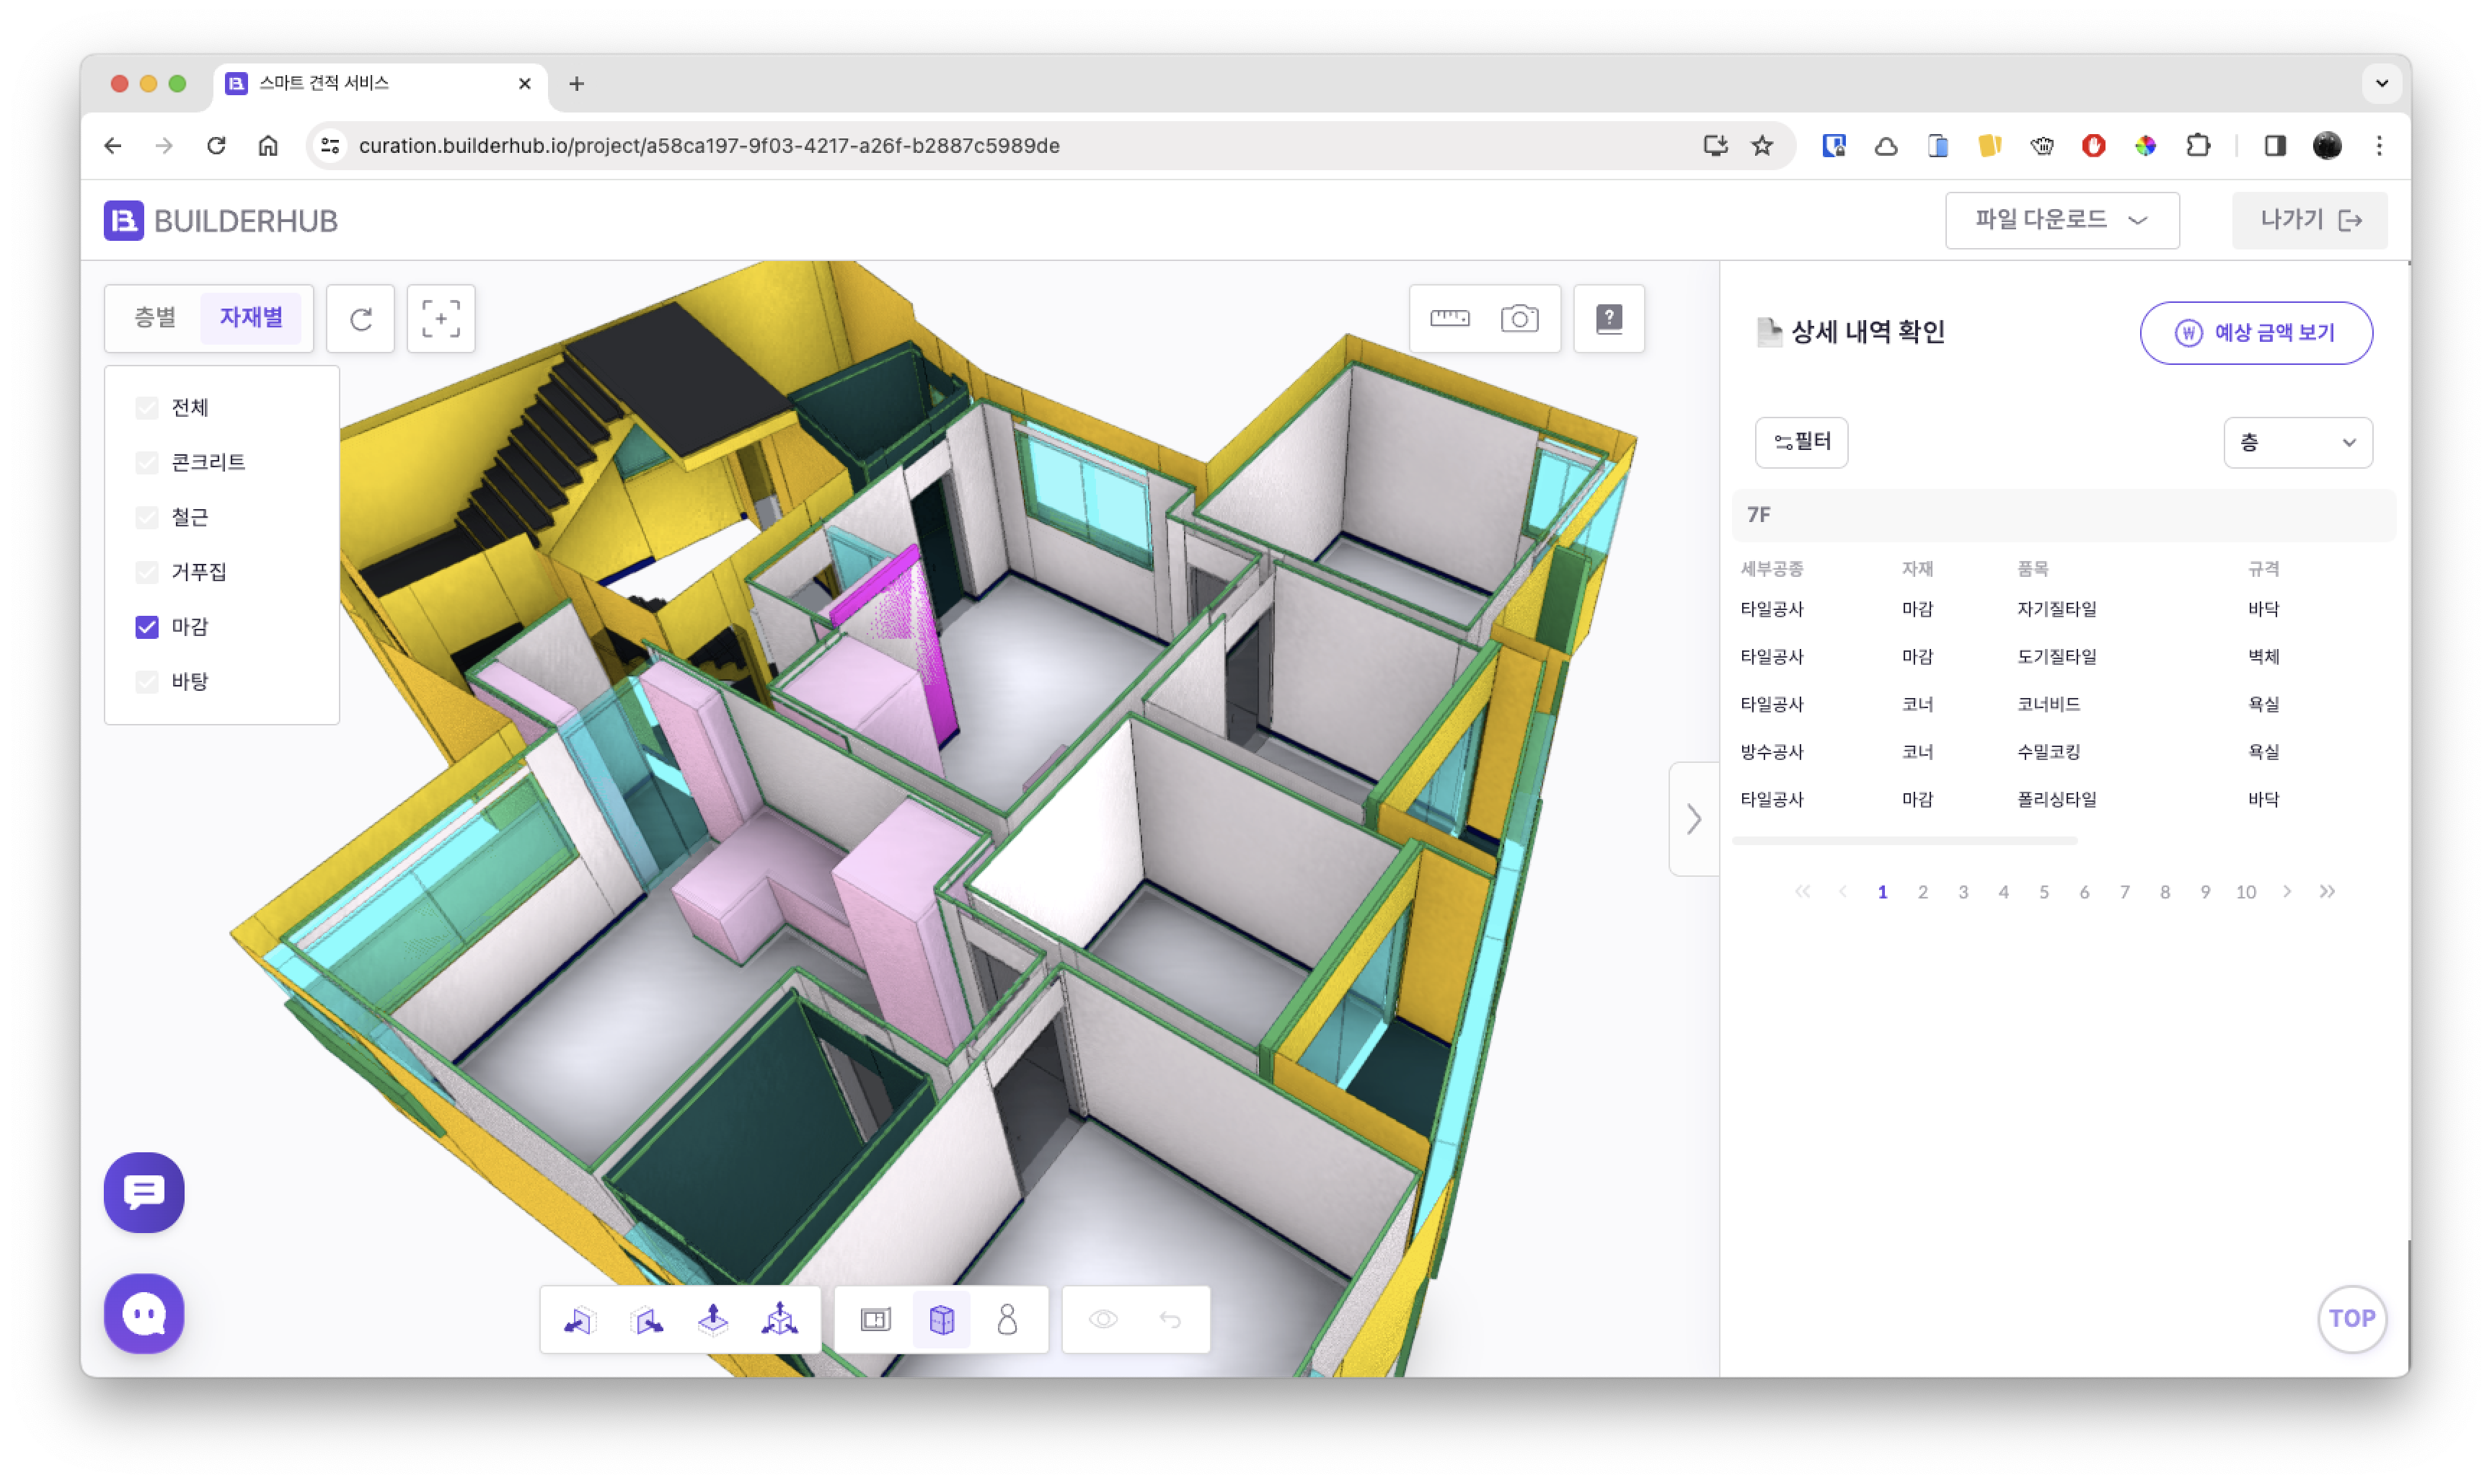
\includegraphics[width=0.35\textwidth]{images/builderhub-curation-filter-floor.png}
					            \caption*{Floor filter}
				            }\qquad
				            \parbox{0.35\textwidth}{
					            \centering
					            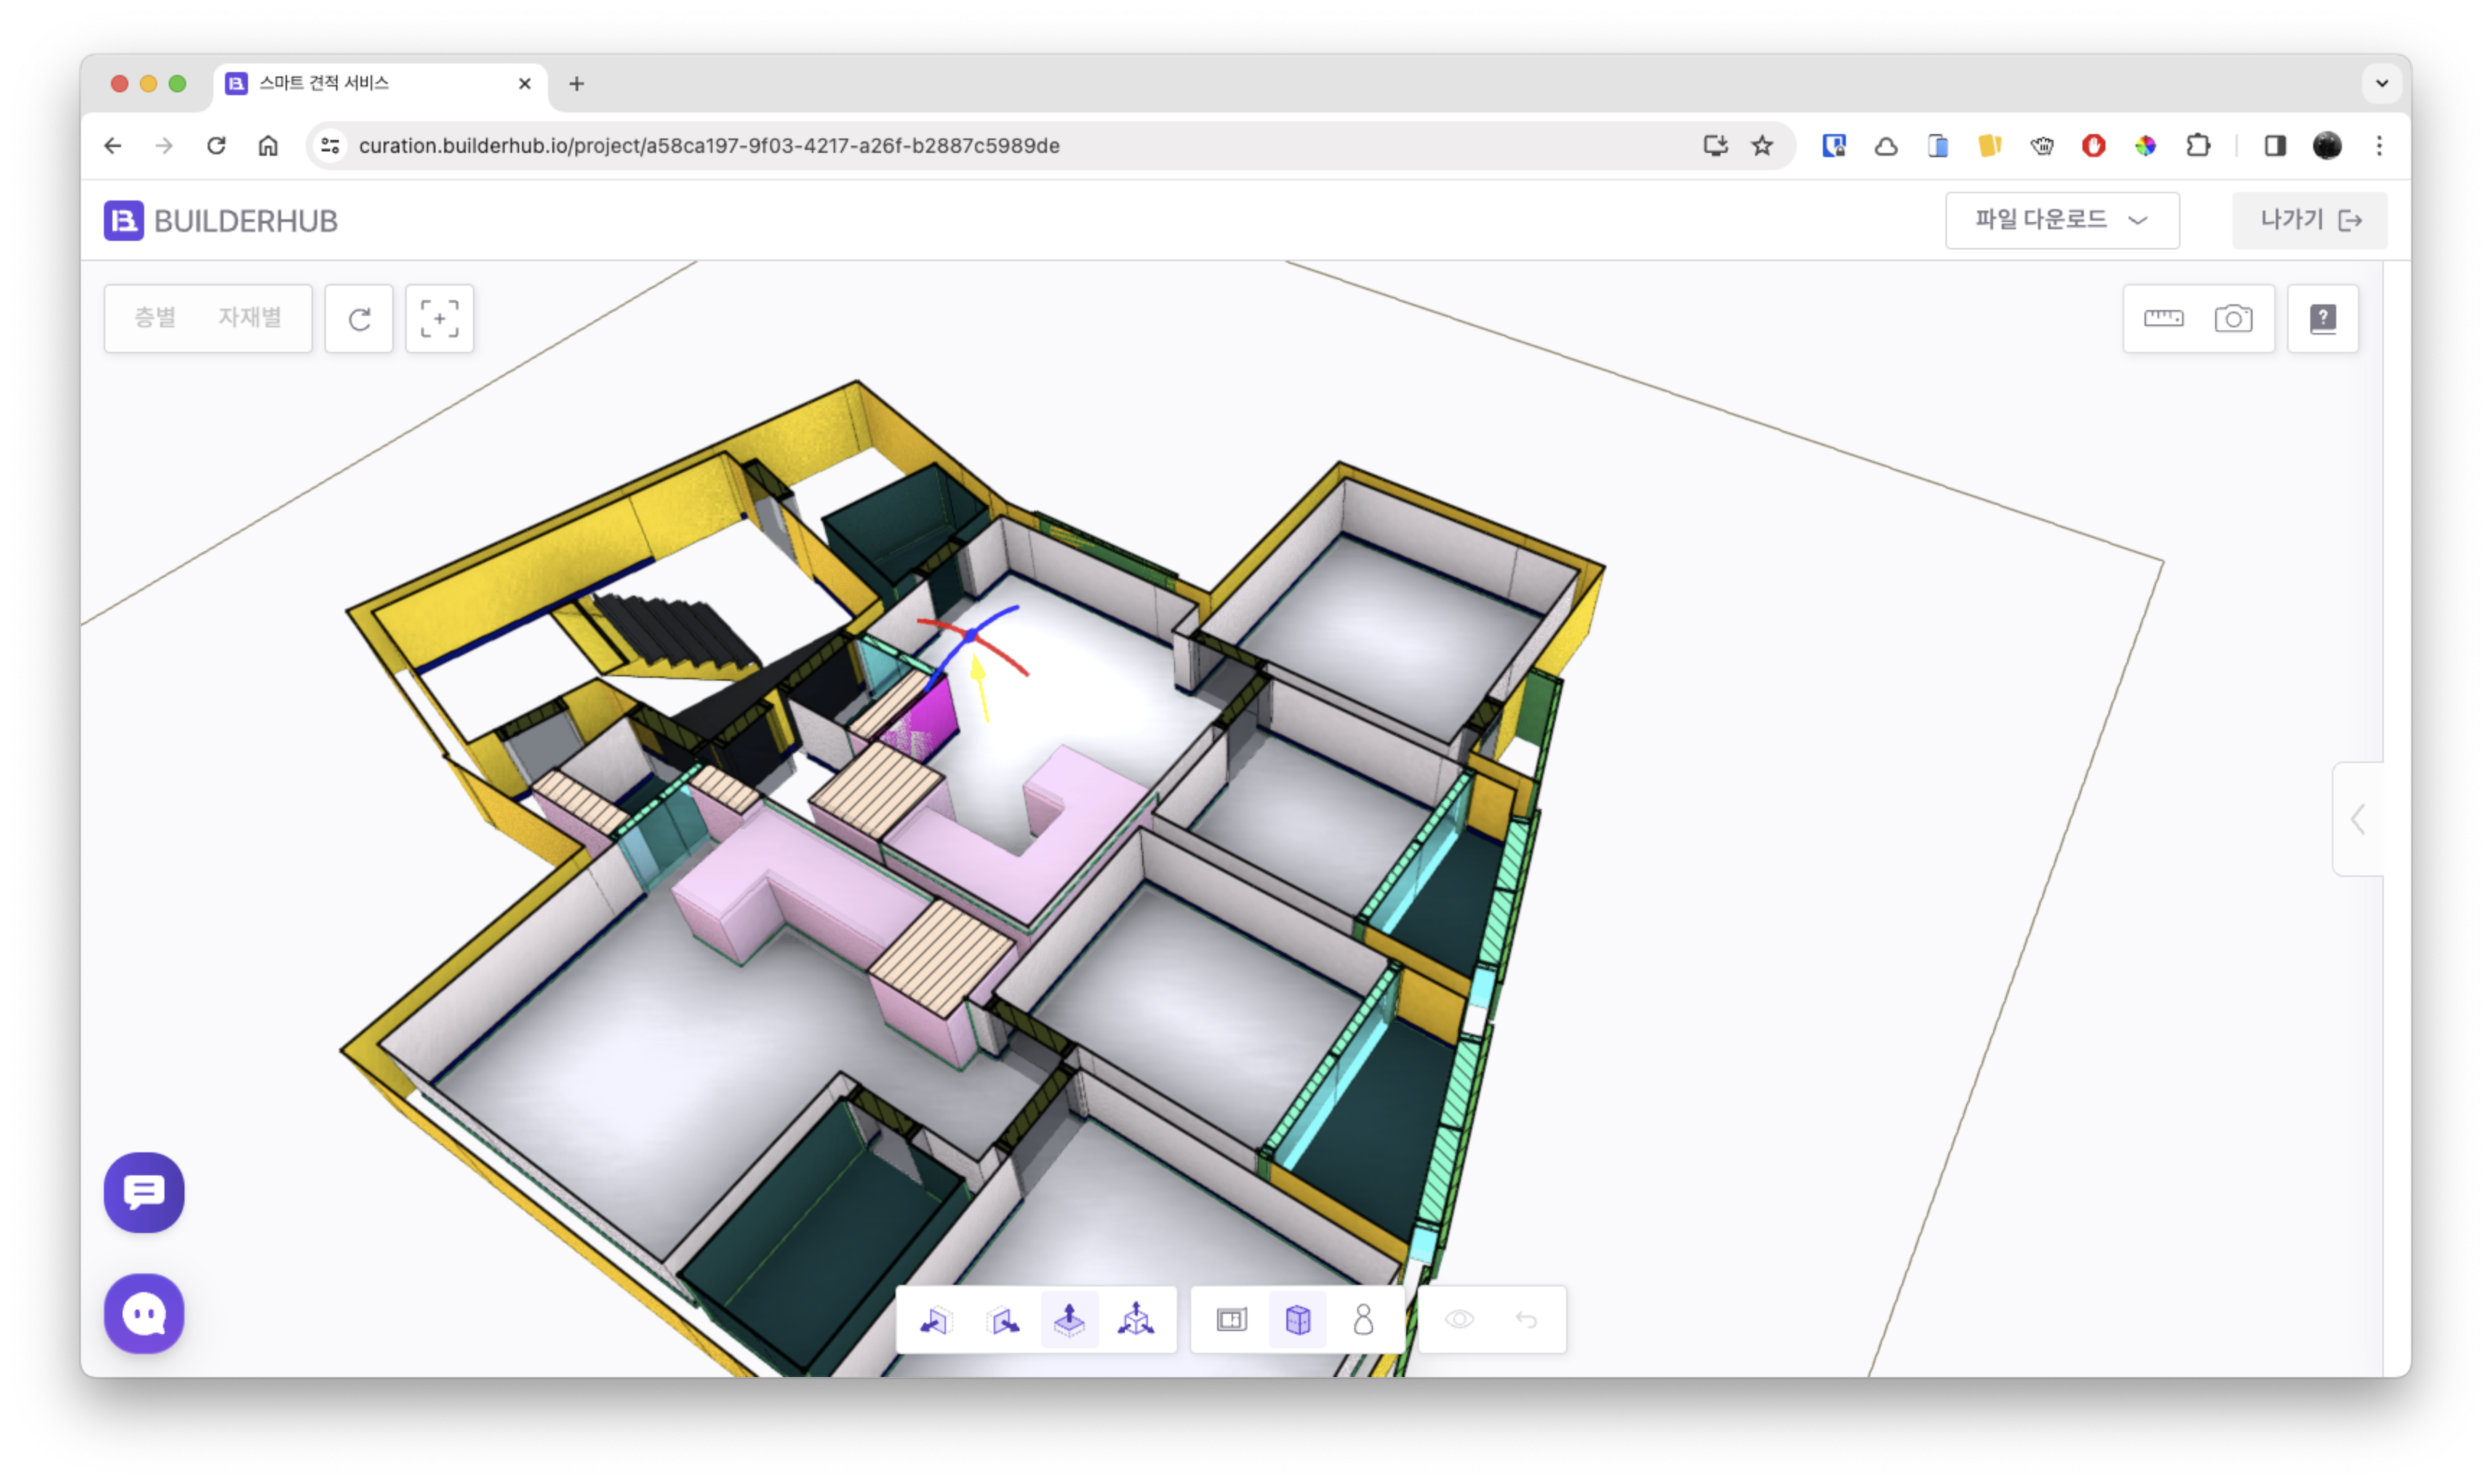
\includegraphics[width=0.35\textwidth]{images/builderhub-curation-section-view.png}
					            \caption*{Section view}
				            }\qquad
				            \parbox{0.35\textwidth}{
					            \centering
					            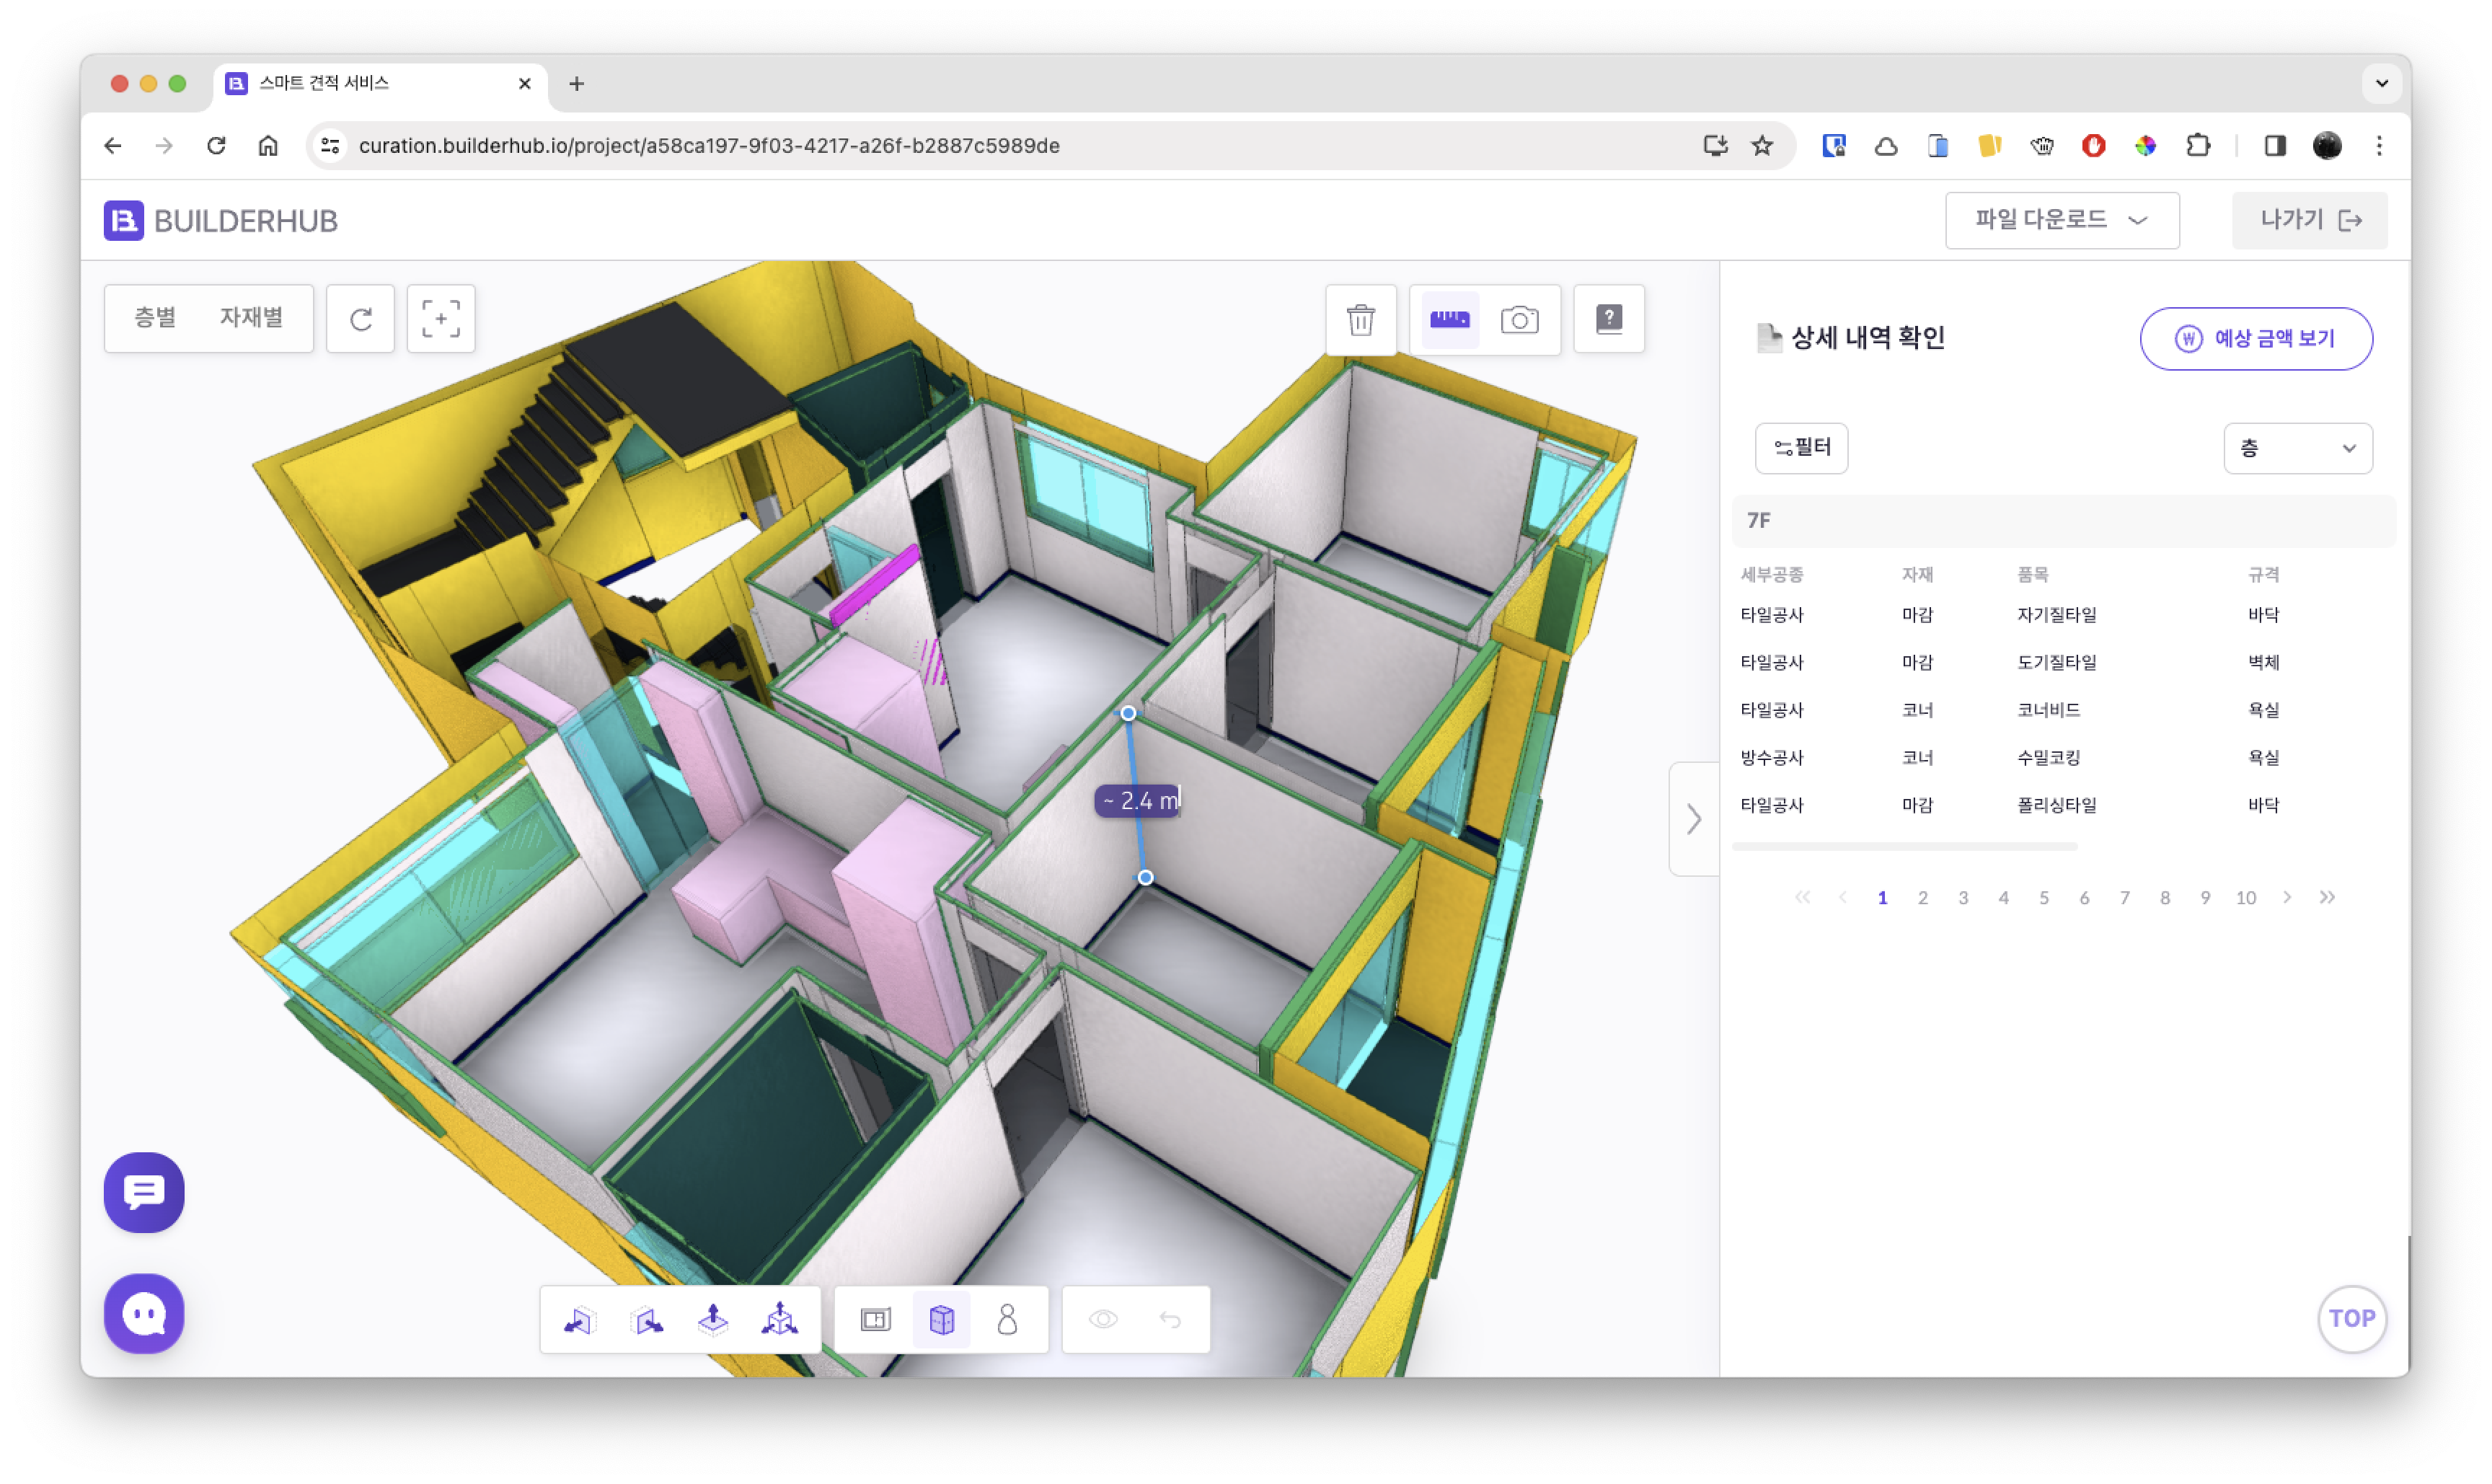
\includegraphics[width=0.35\textwidth]{images/builderhub-curation-measurement.png}
					            \caption*{Measurement}
				            }\qquad
				            \parbox{0.35\textwidth}{
					            \centering
					            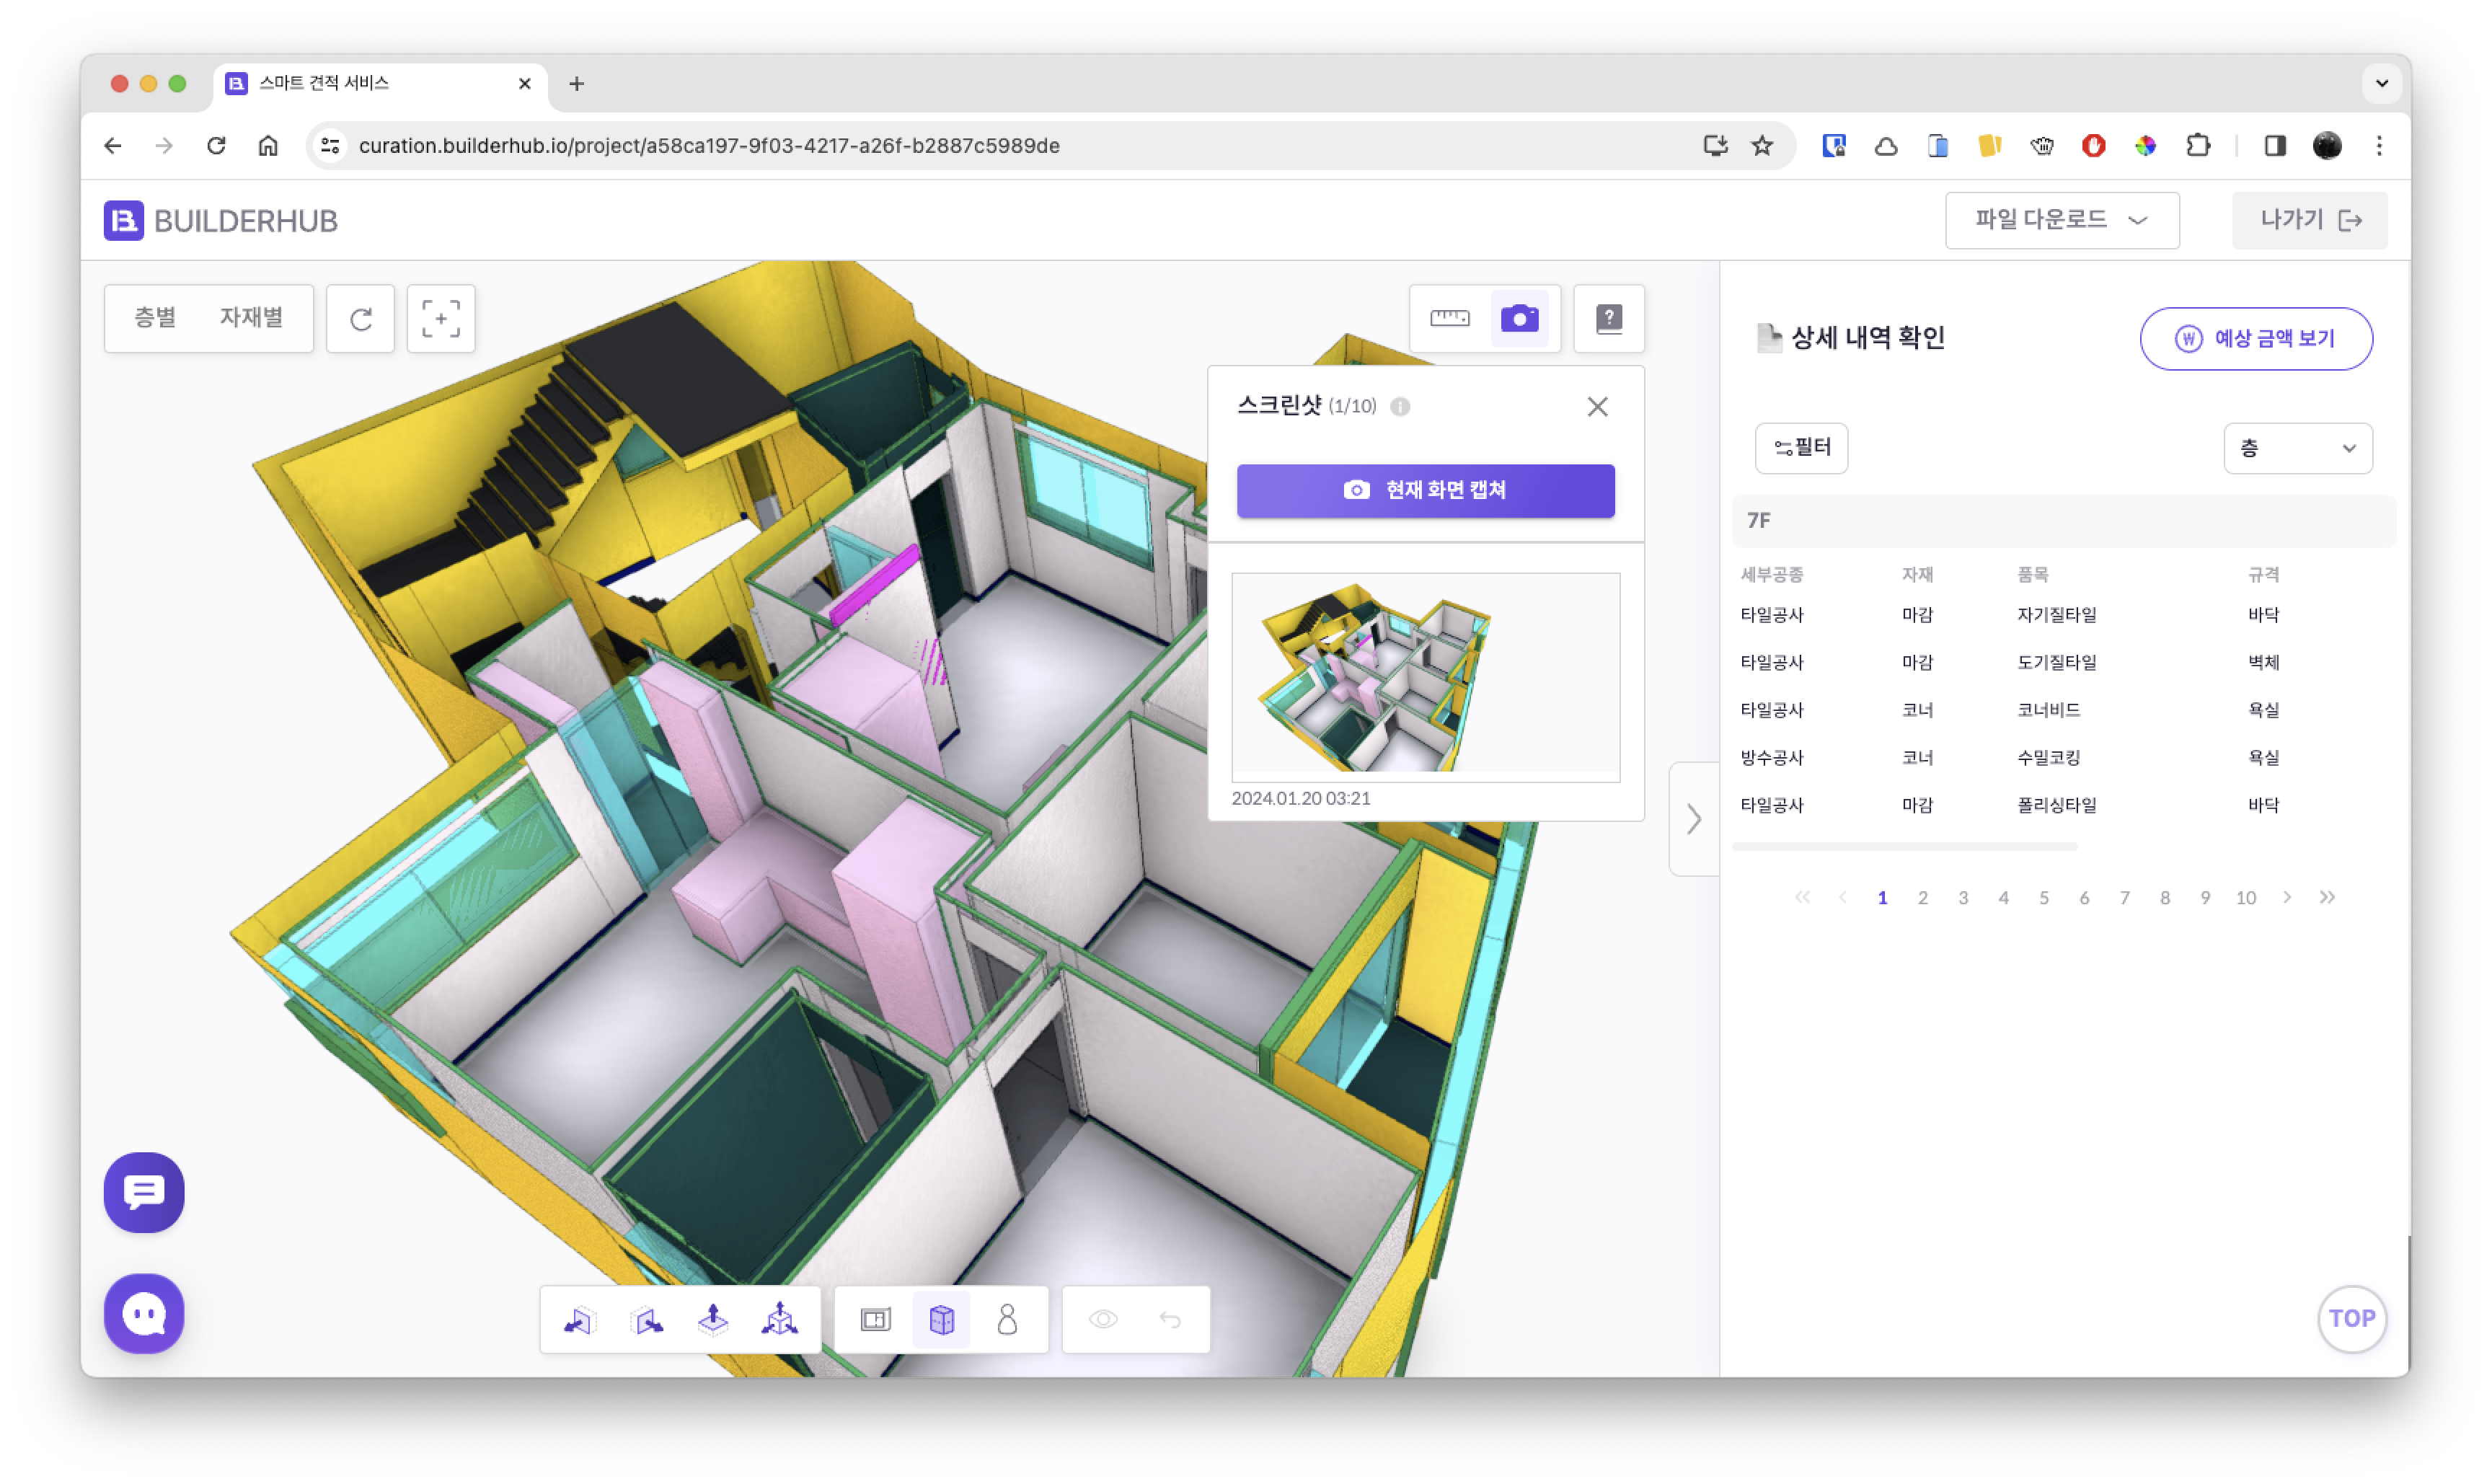
\includegraphics[width=0.35\textwidth]{images/builderhub-curation-screenshot.png}
					            \caption*{Screen Capture}
				            }
				            \parbox{0.35\textwidth}{
					            \centering
					            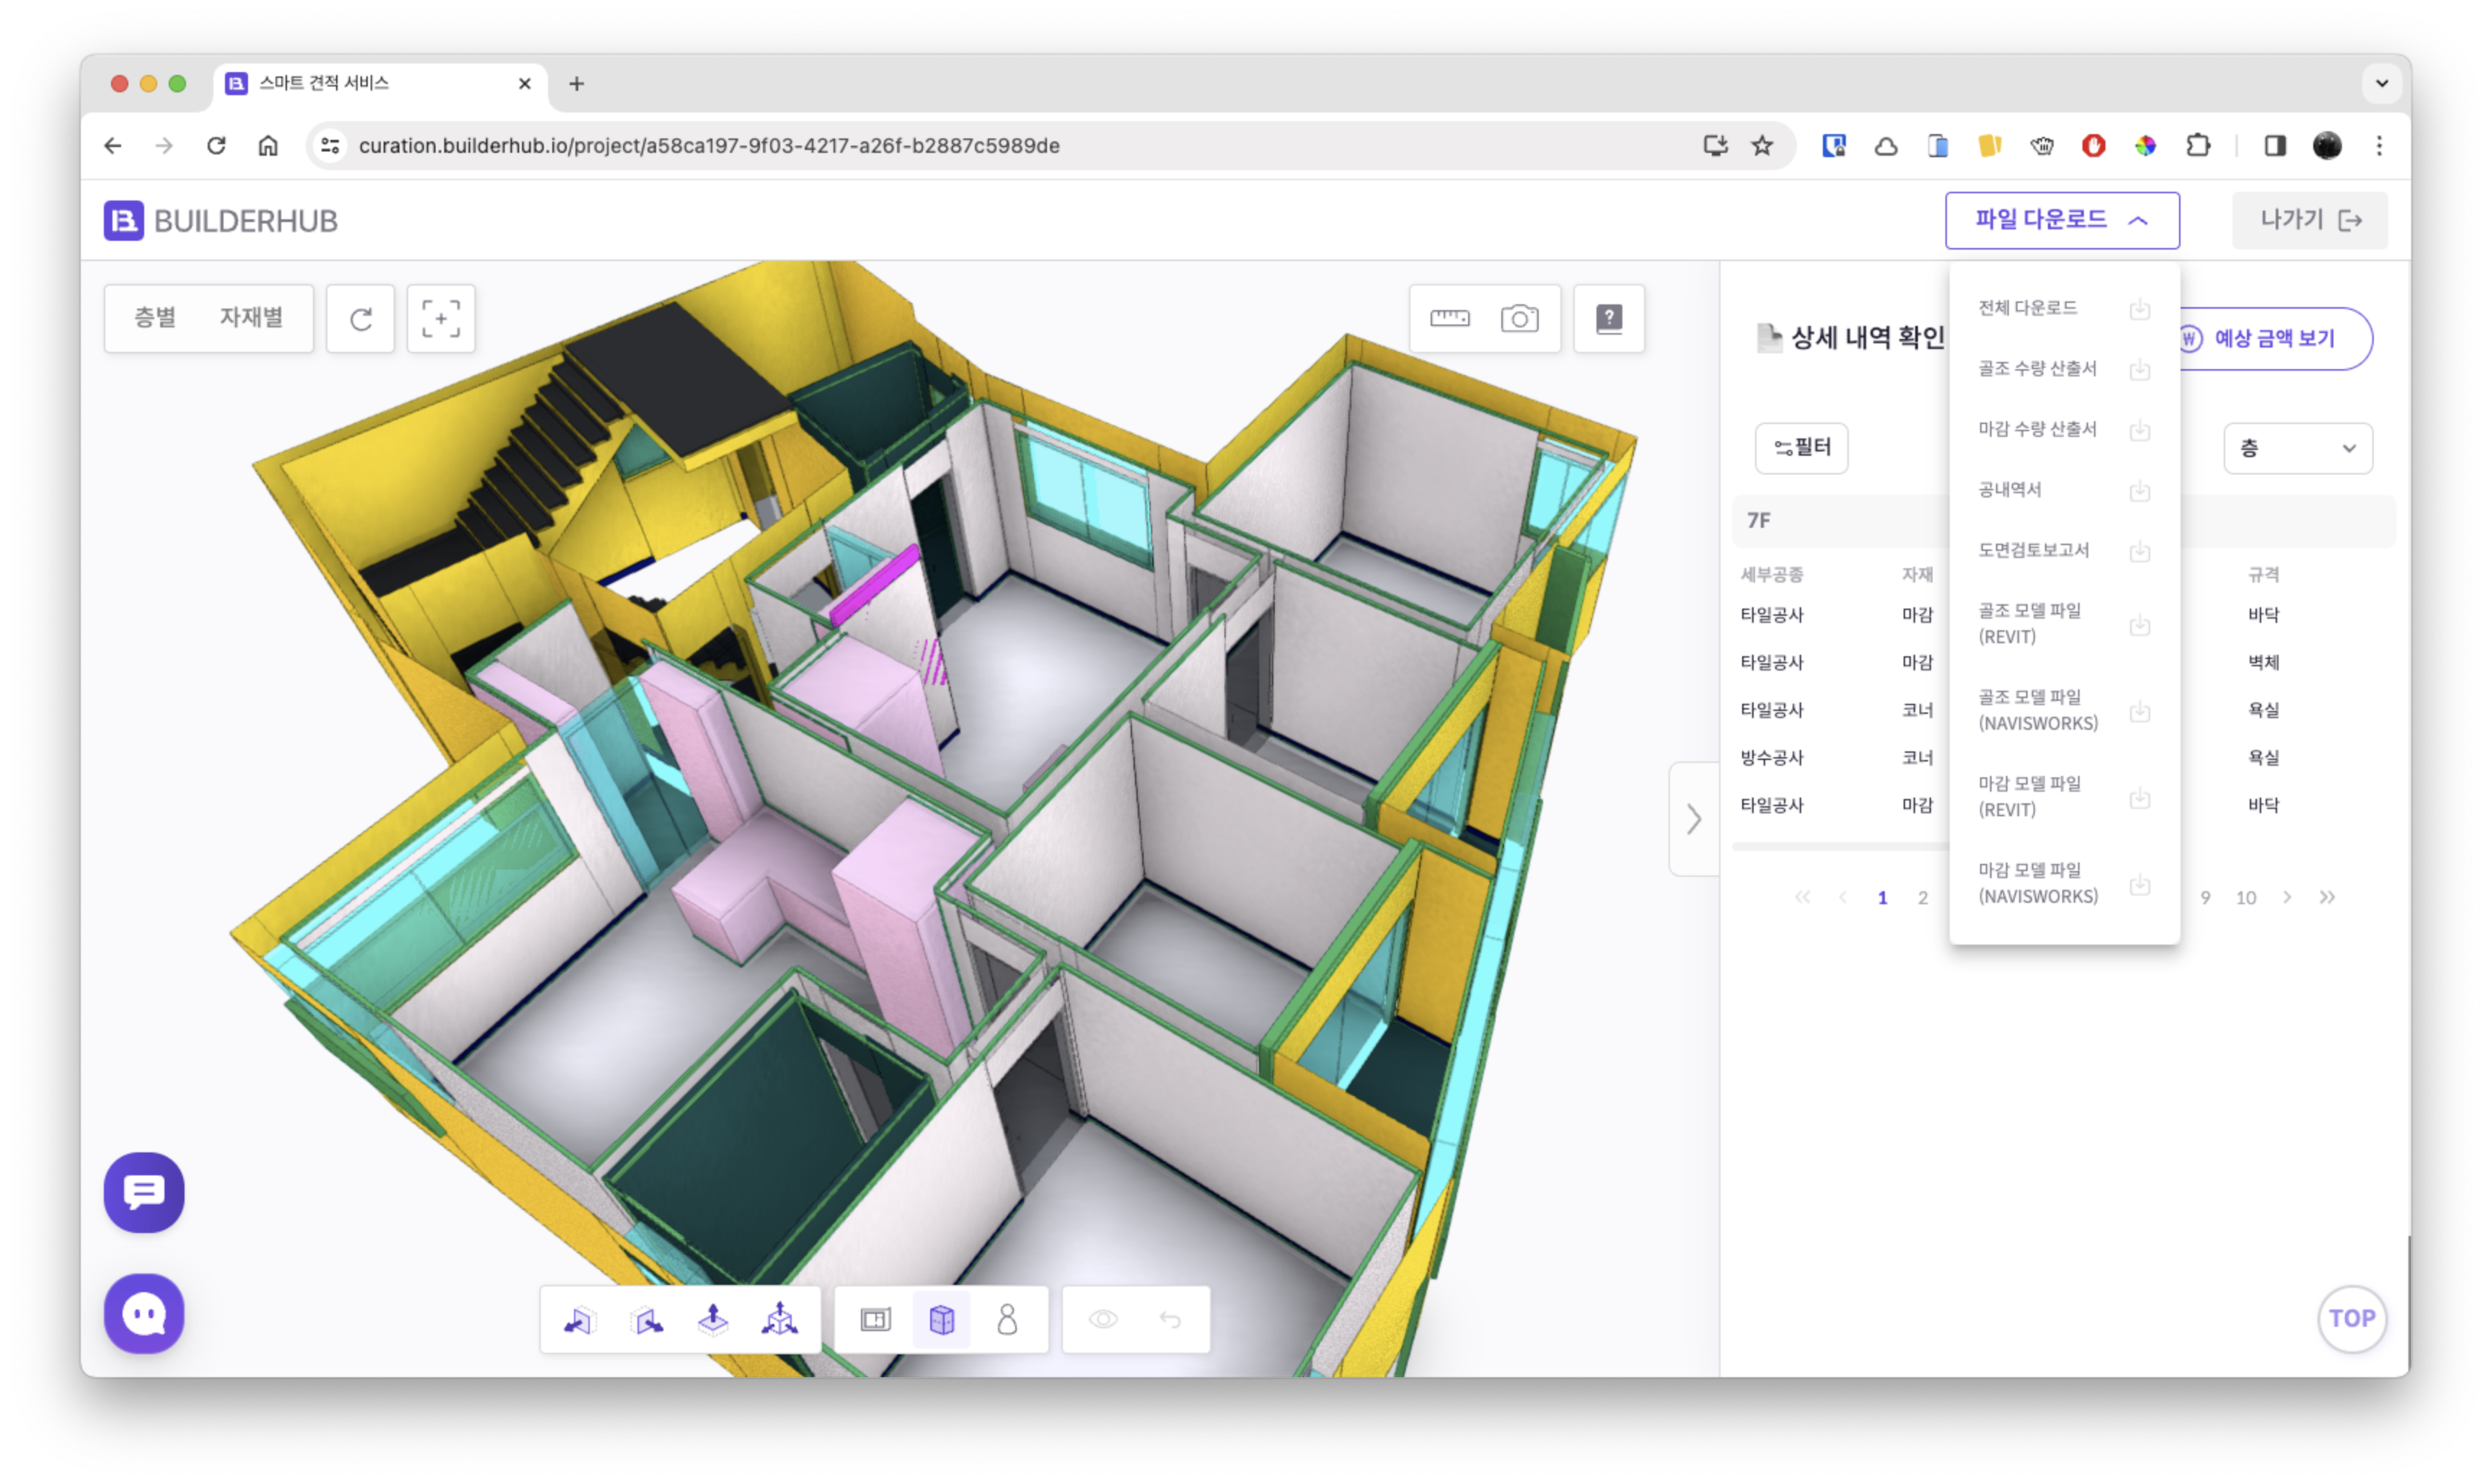
\includegraphics[width=0.35\textwidth]{images/builderhub-curation-download.png}
					            \caption*{Download assets}
				            }\qquad
				            \parbox{0.35\textwidth}{
					            \centering
					            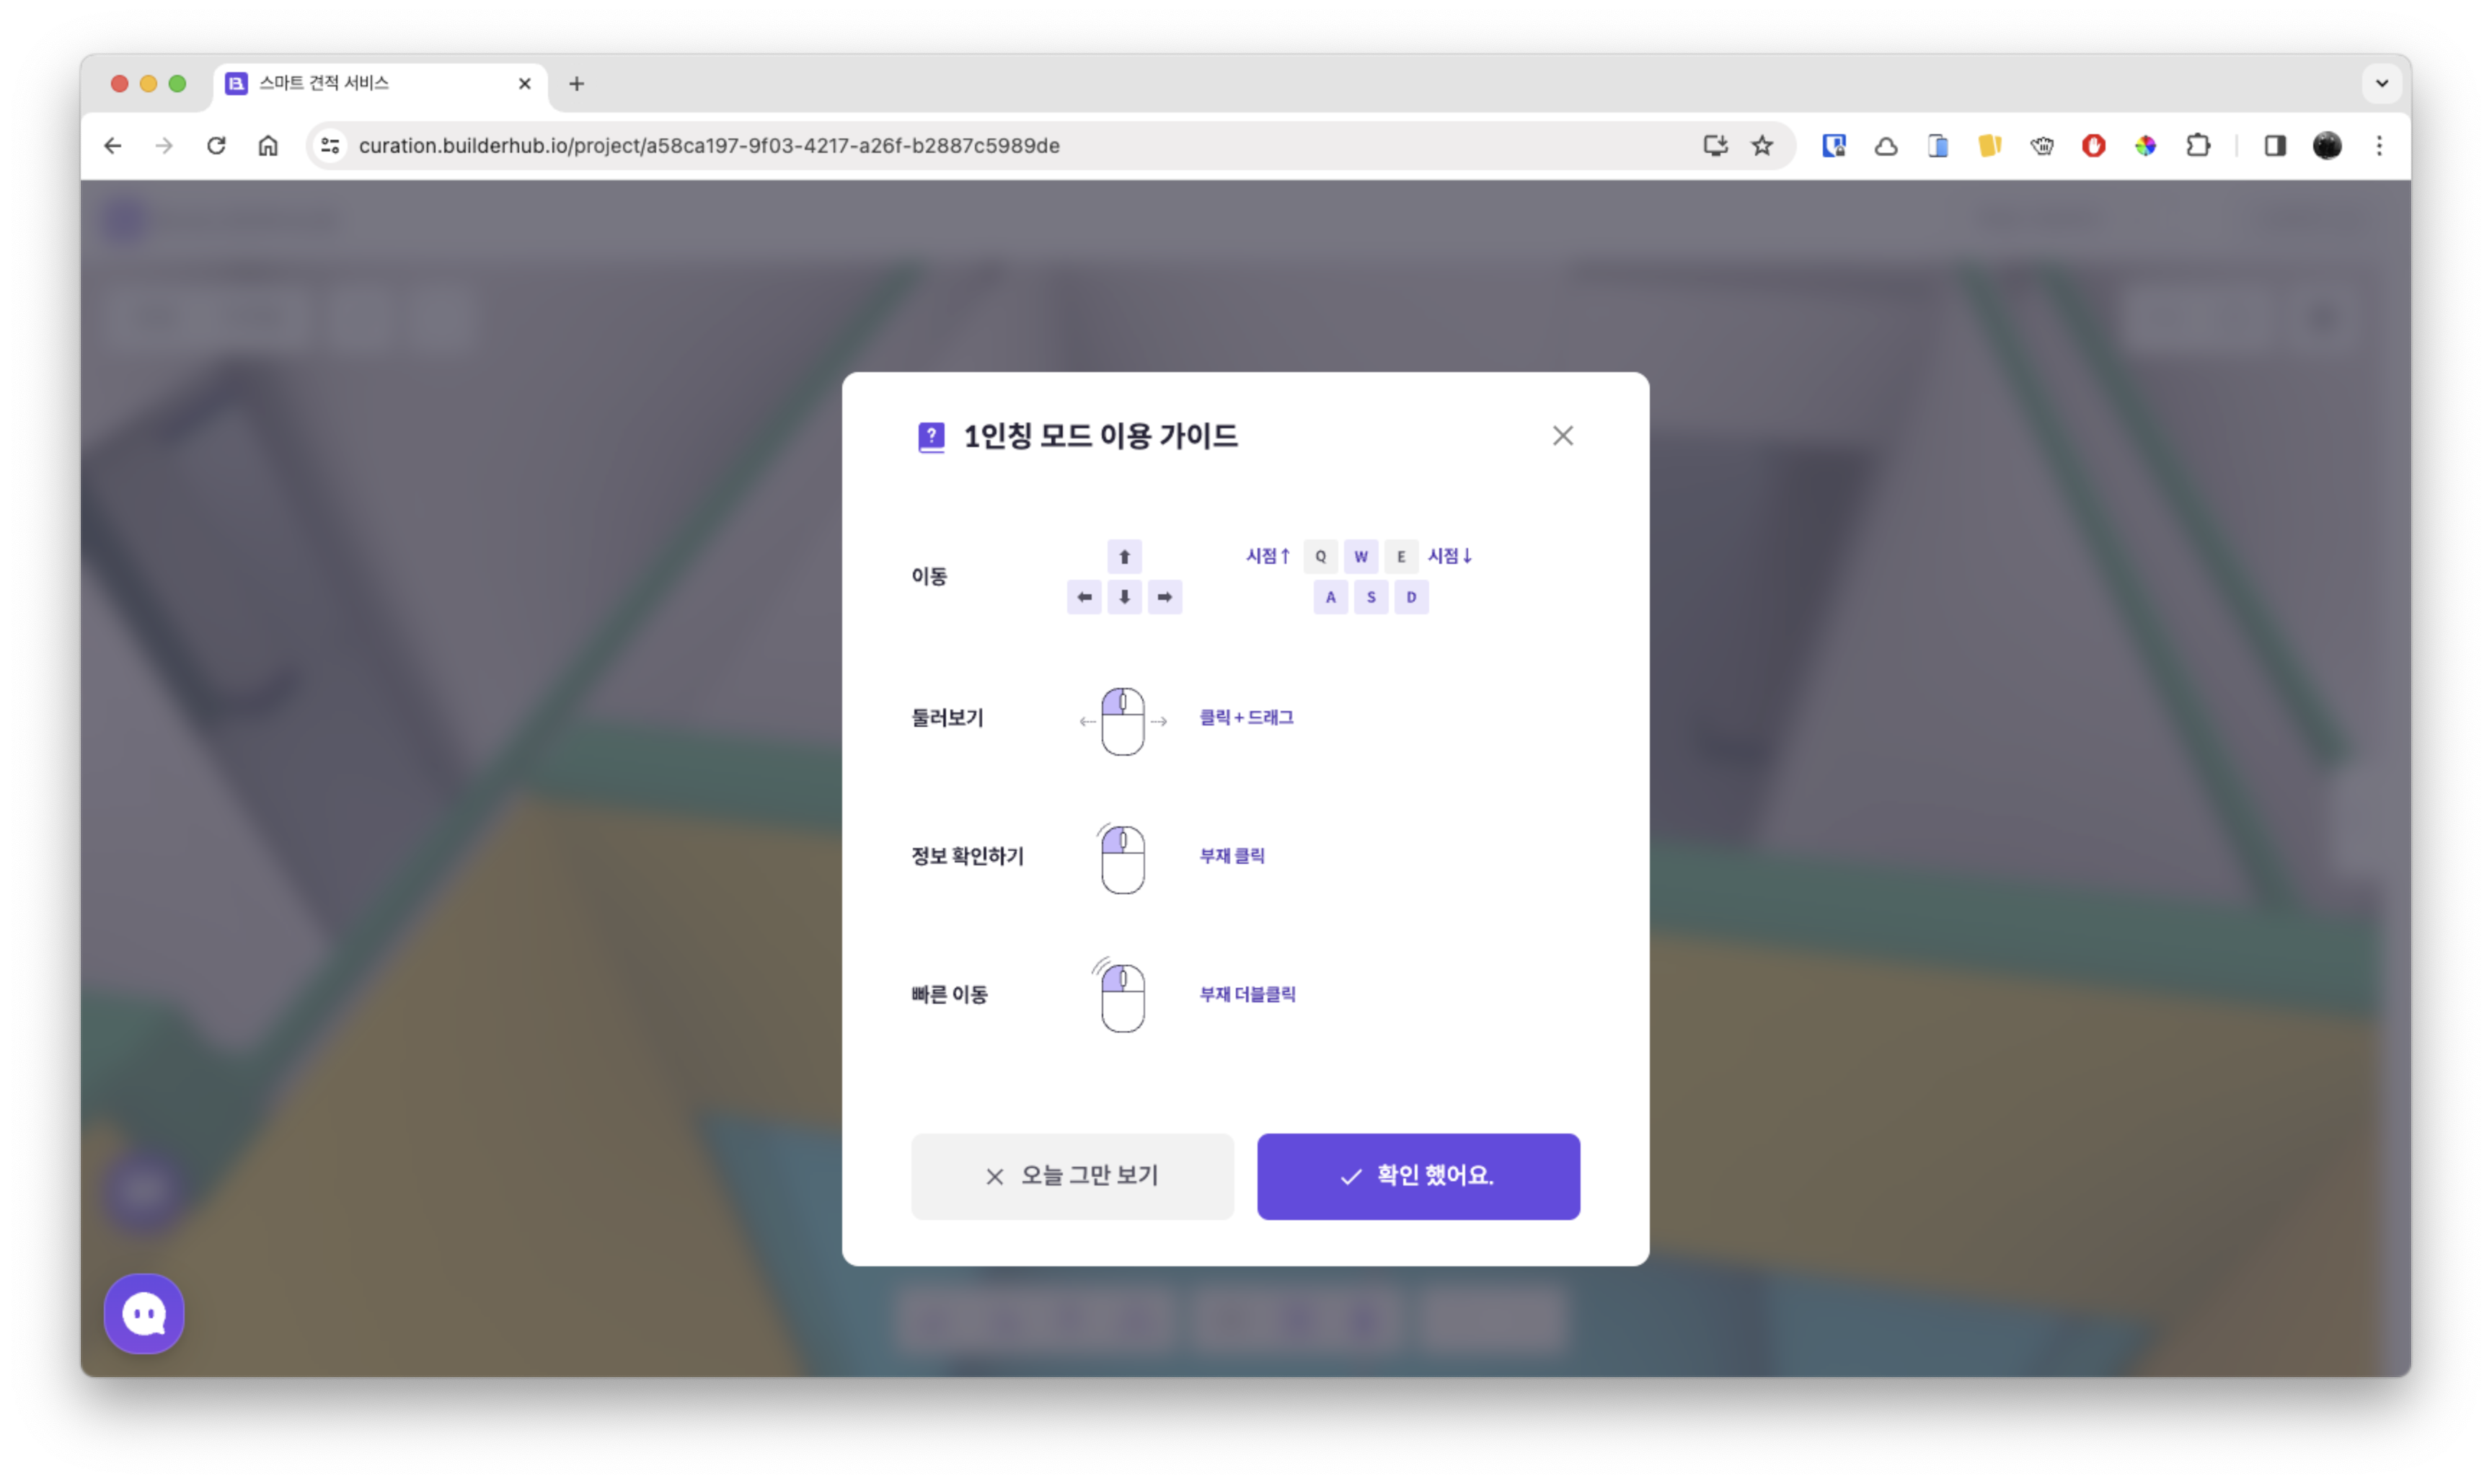
\includegraphics[width=0.35\textwidth]{images/builderhub-curation-first-person-view-1.png}
					            \caption*{First-person view guide}
				            }\qquad
				            \parbox{0.35\textwidth}{
					            \centering
					            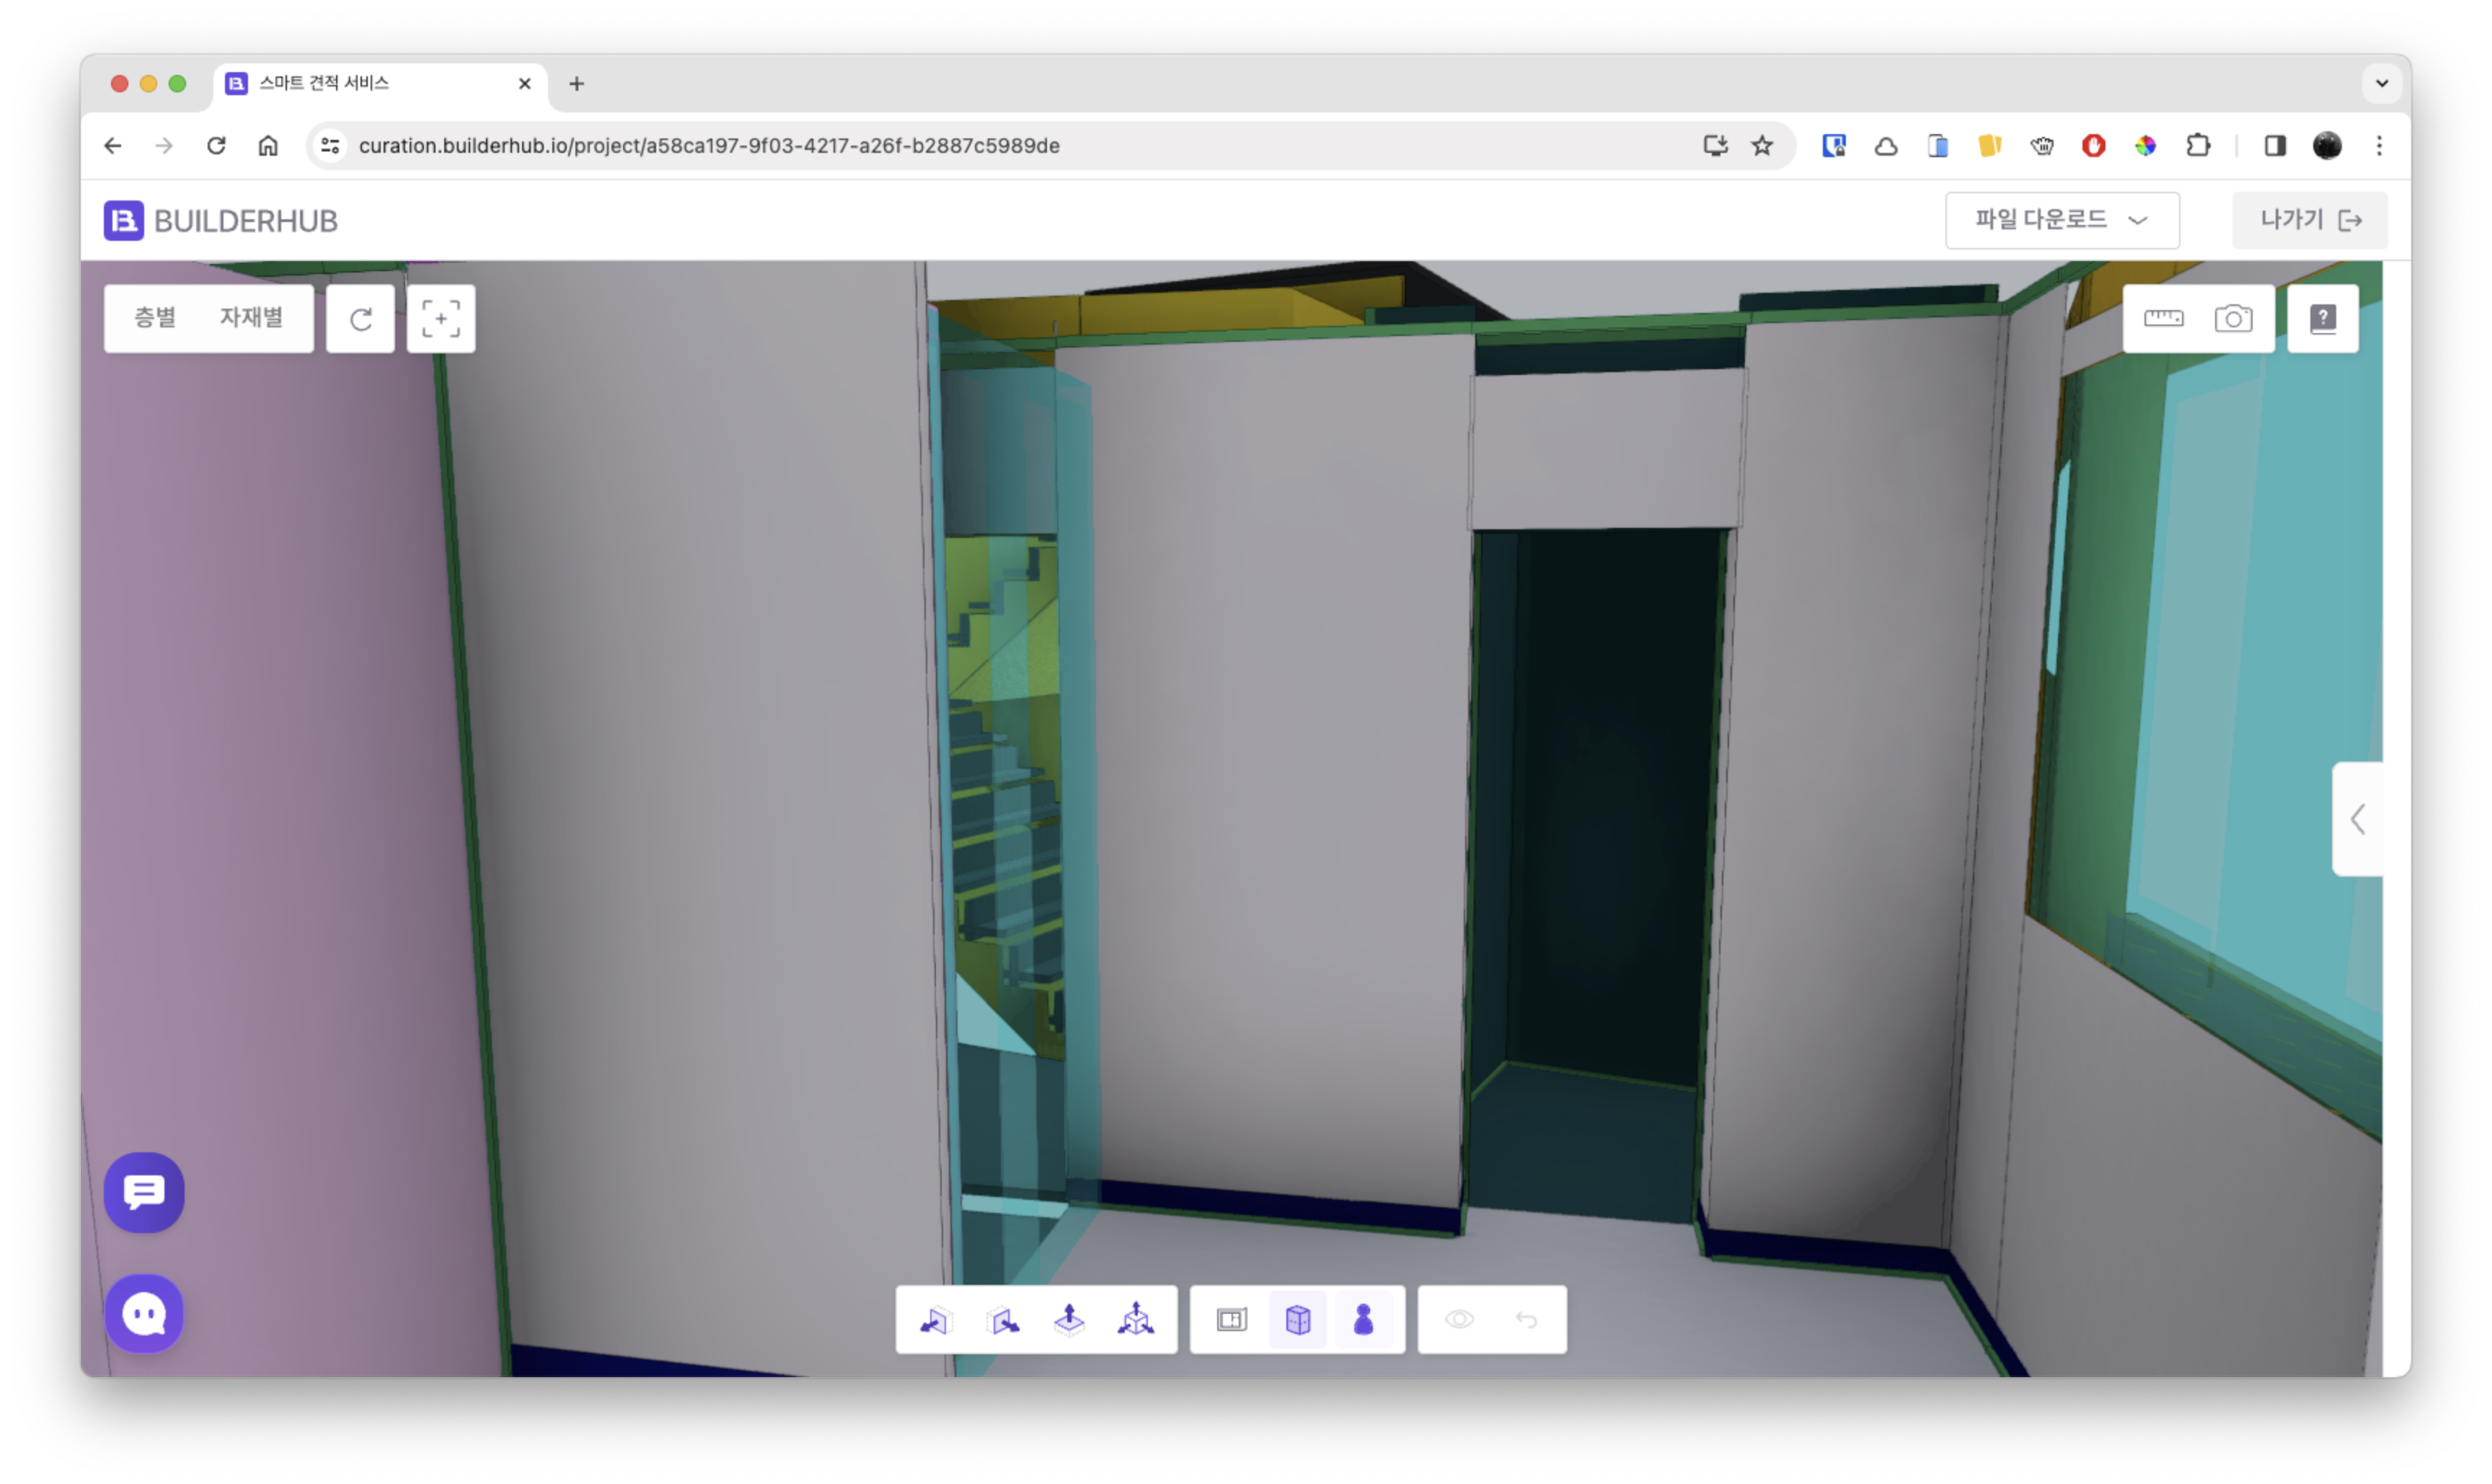
\includegraphics[width=0.35\textwidth]{images/builderhub-curation-first-person-view-2.png}
					            \caption*{Frist-person view control}
				            }\qquad
				            \parbox{0.35\textwidth}{
					            \centering
					            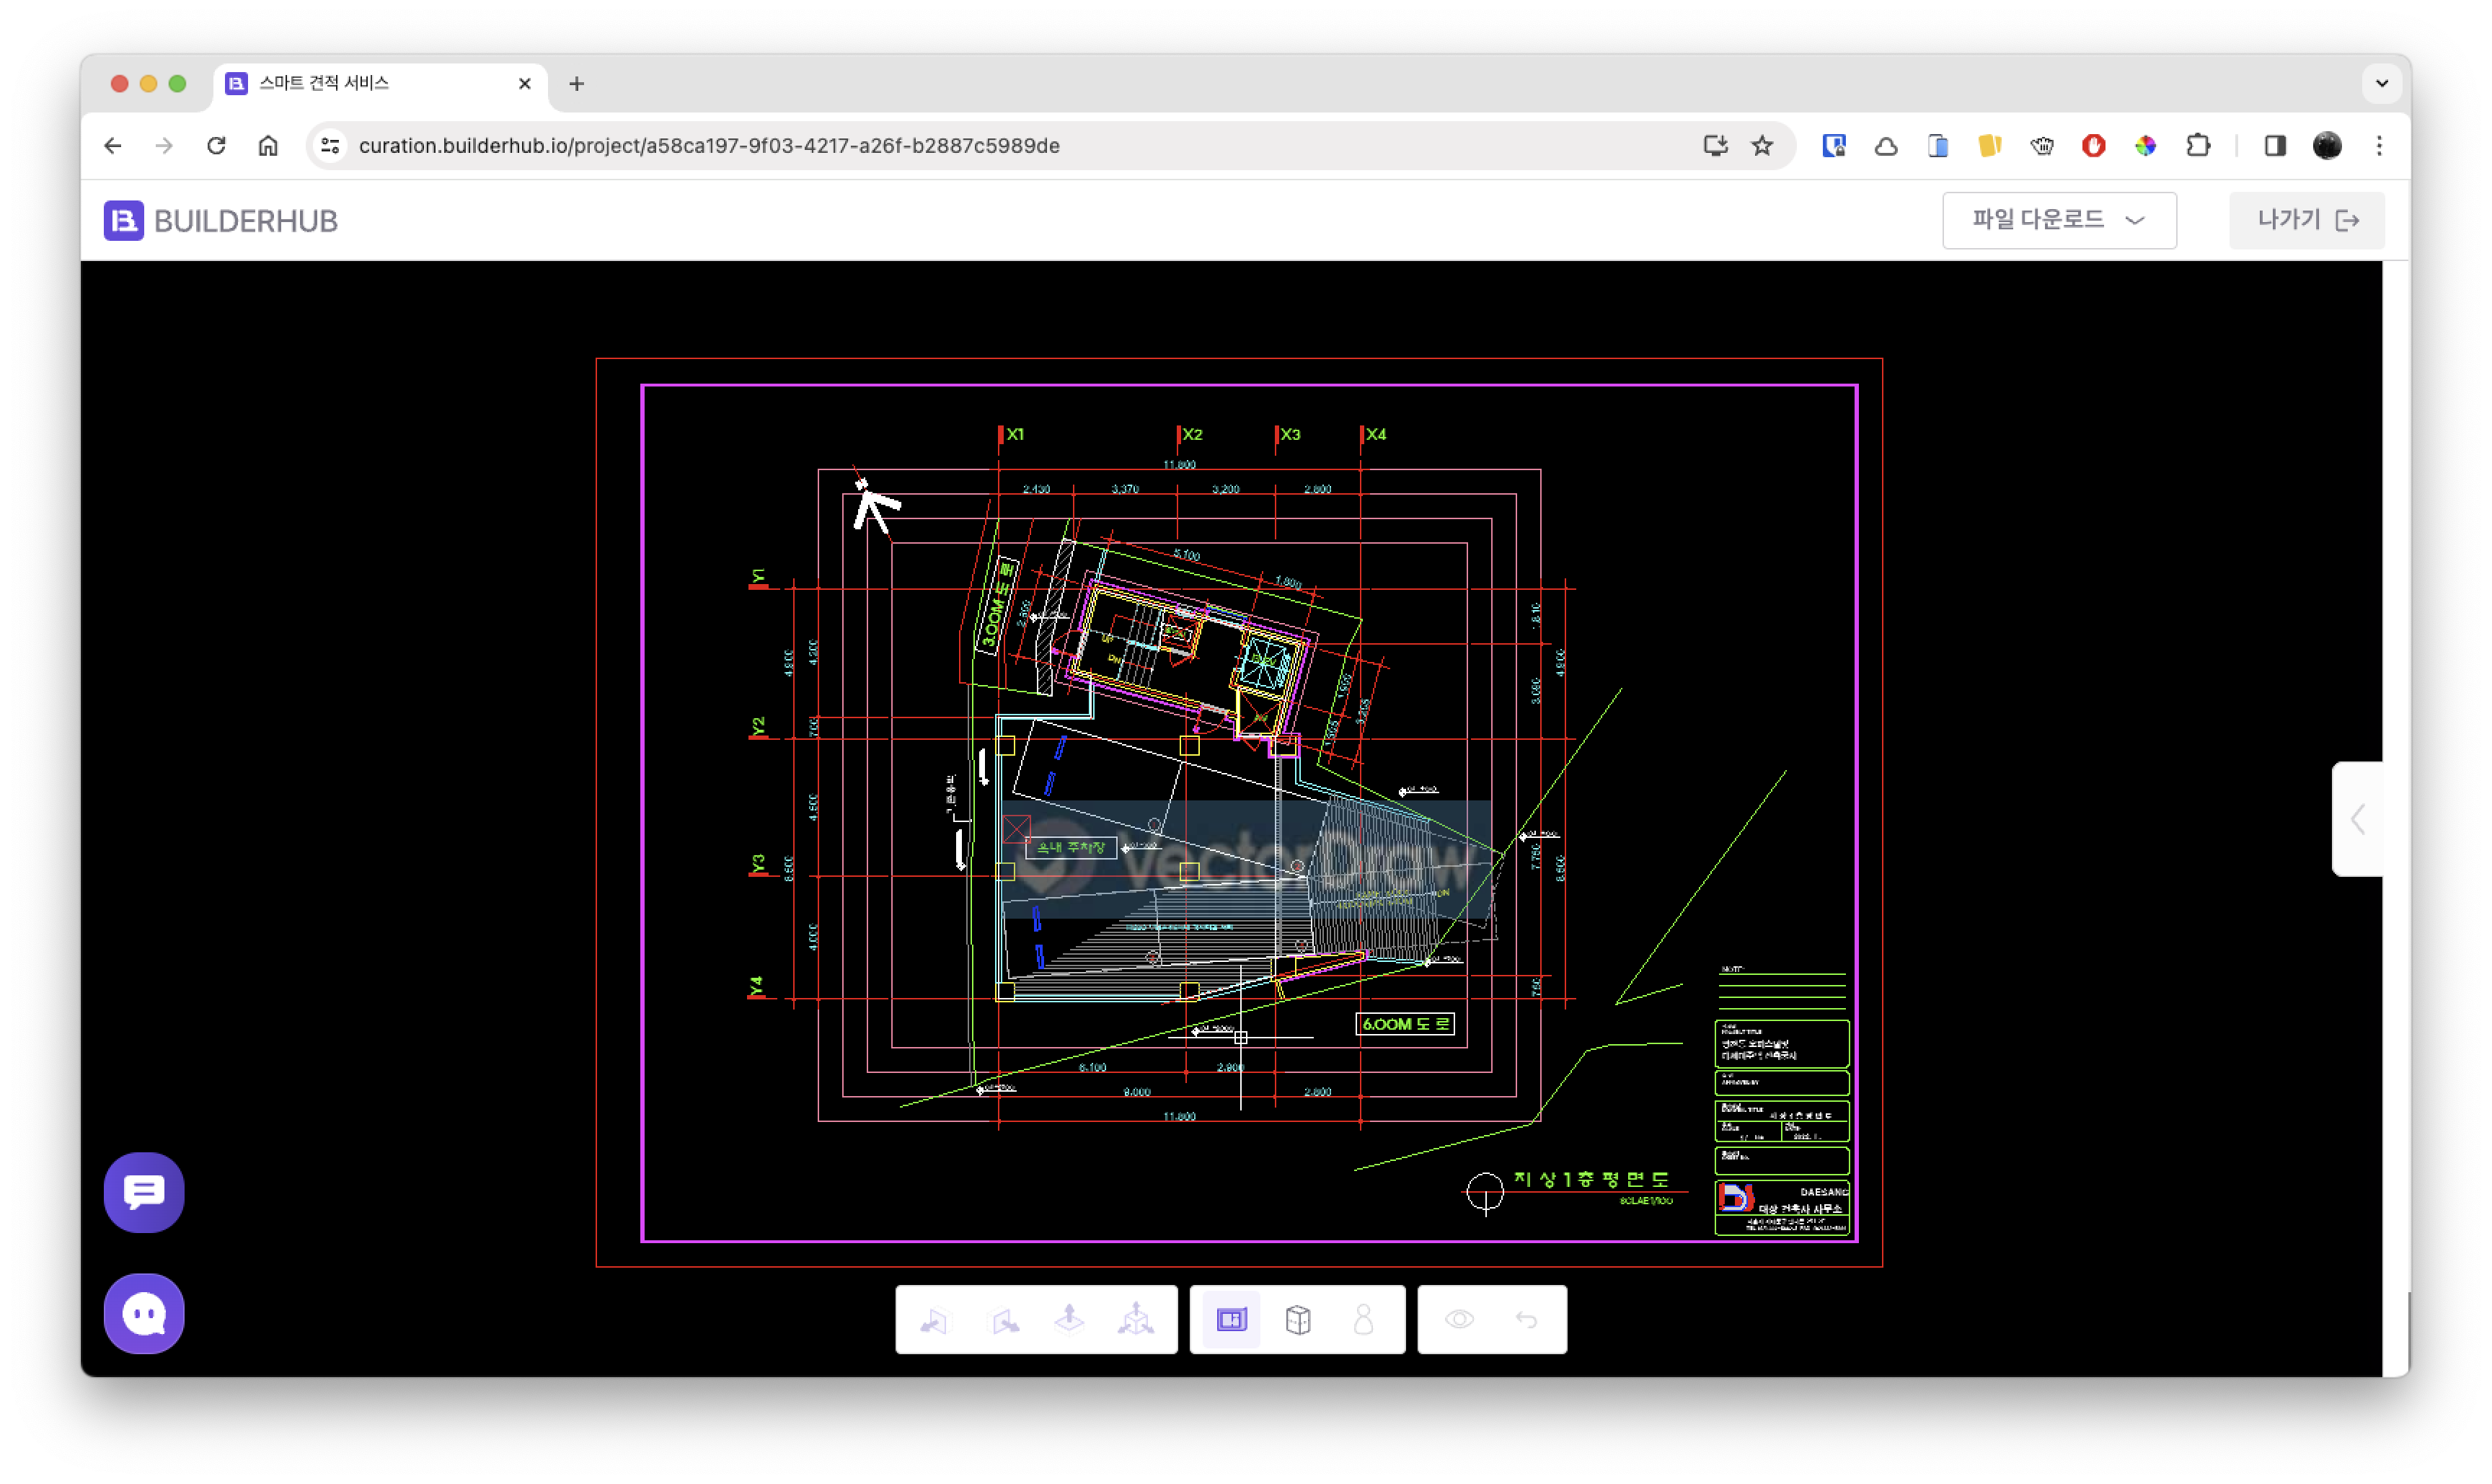
\includegraphics[width=0.35\textwidth]{images/builderhub-curation-2d-view.png}
					            \caption*{2D drawing view}
				            }
			            \end{fullwidth}
		            \end{figure}
		      \item \textbf{\href{https://partners.builderhub.io/}{파트너 서비스} 개발}
		            \begin{itemize}
			            \item 파트너 등록 및 검수, 대시보드, 프로필 수정
			            \item 공공 API 및 공공 데이터 연동 파트너 정보 등록, 포트폴리오 등록, 블로그 및 콘텐츠 서비스 (개발중)
		            \end{itemize}
		            \begin{figure}[!ht]
			            \begin{fullwidth}
				            \parbox{0.35\textwidth}{
					            \centering
					            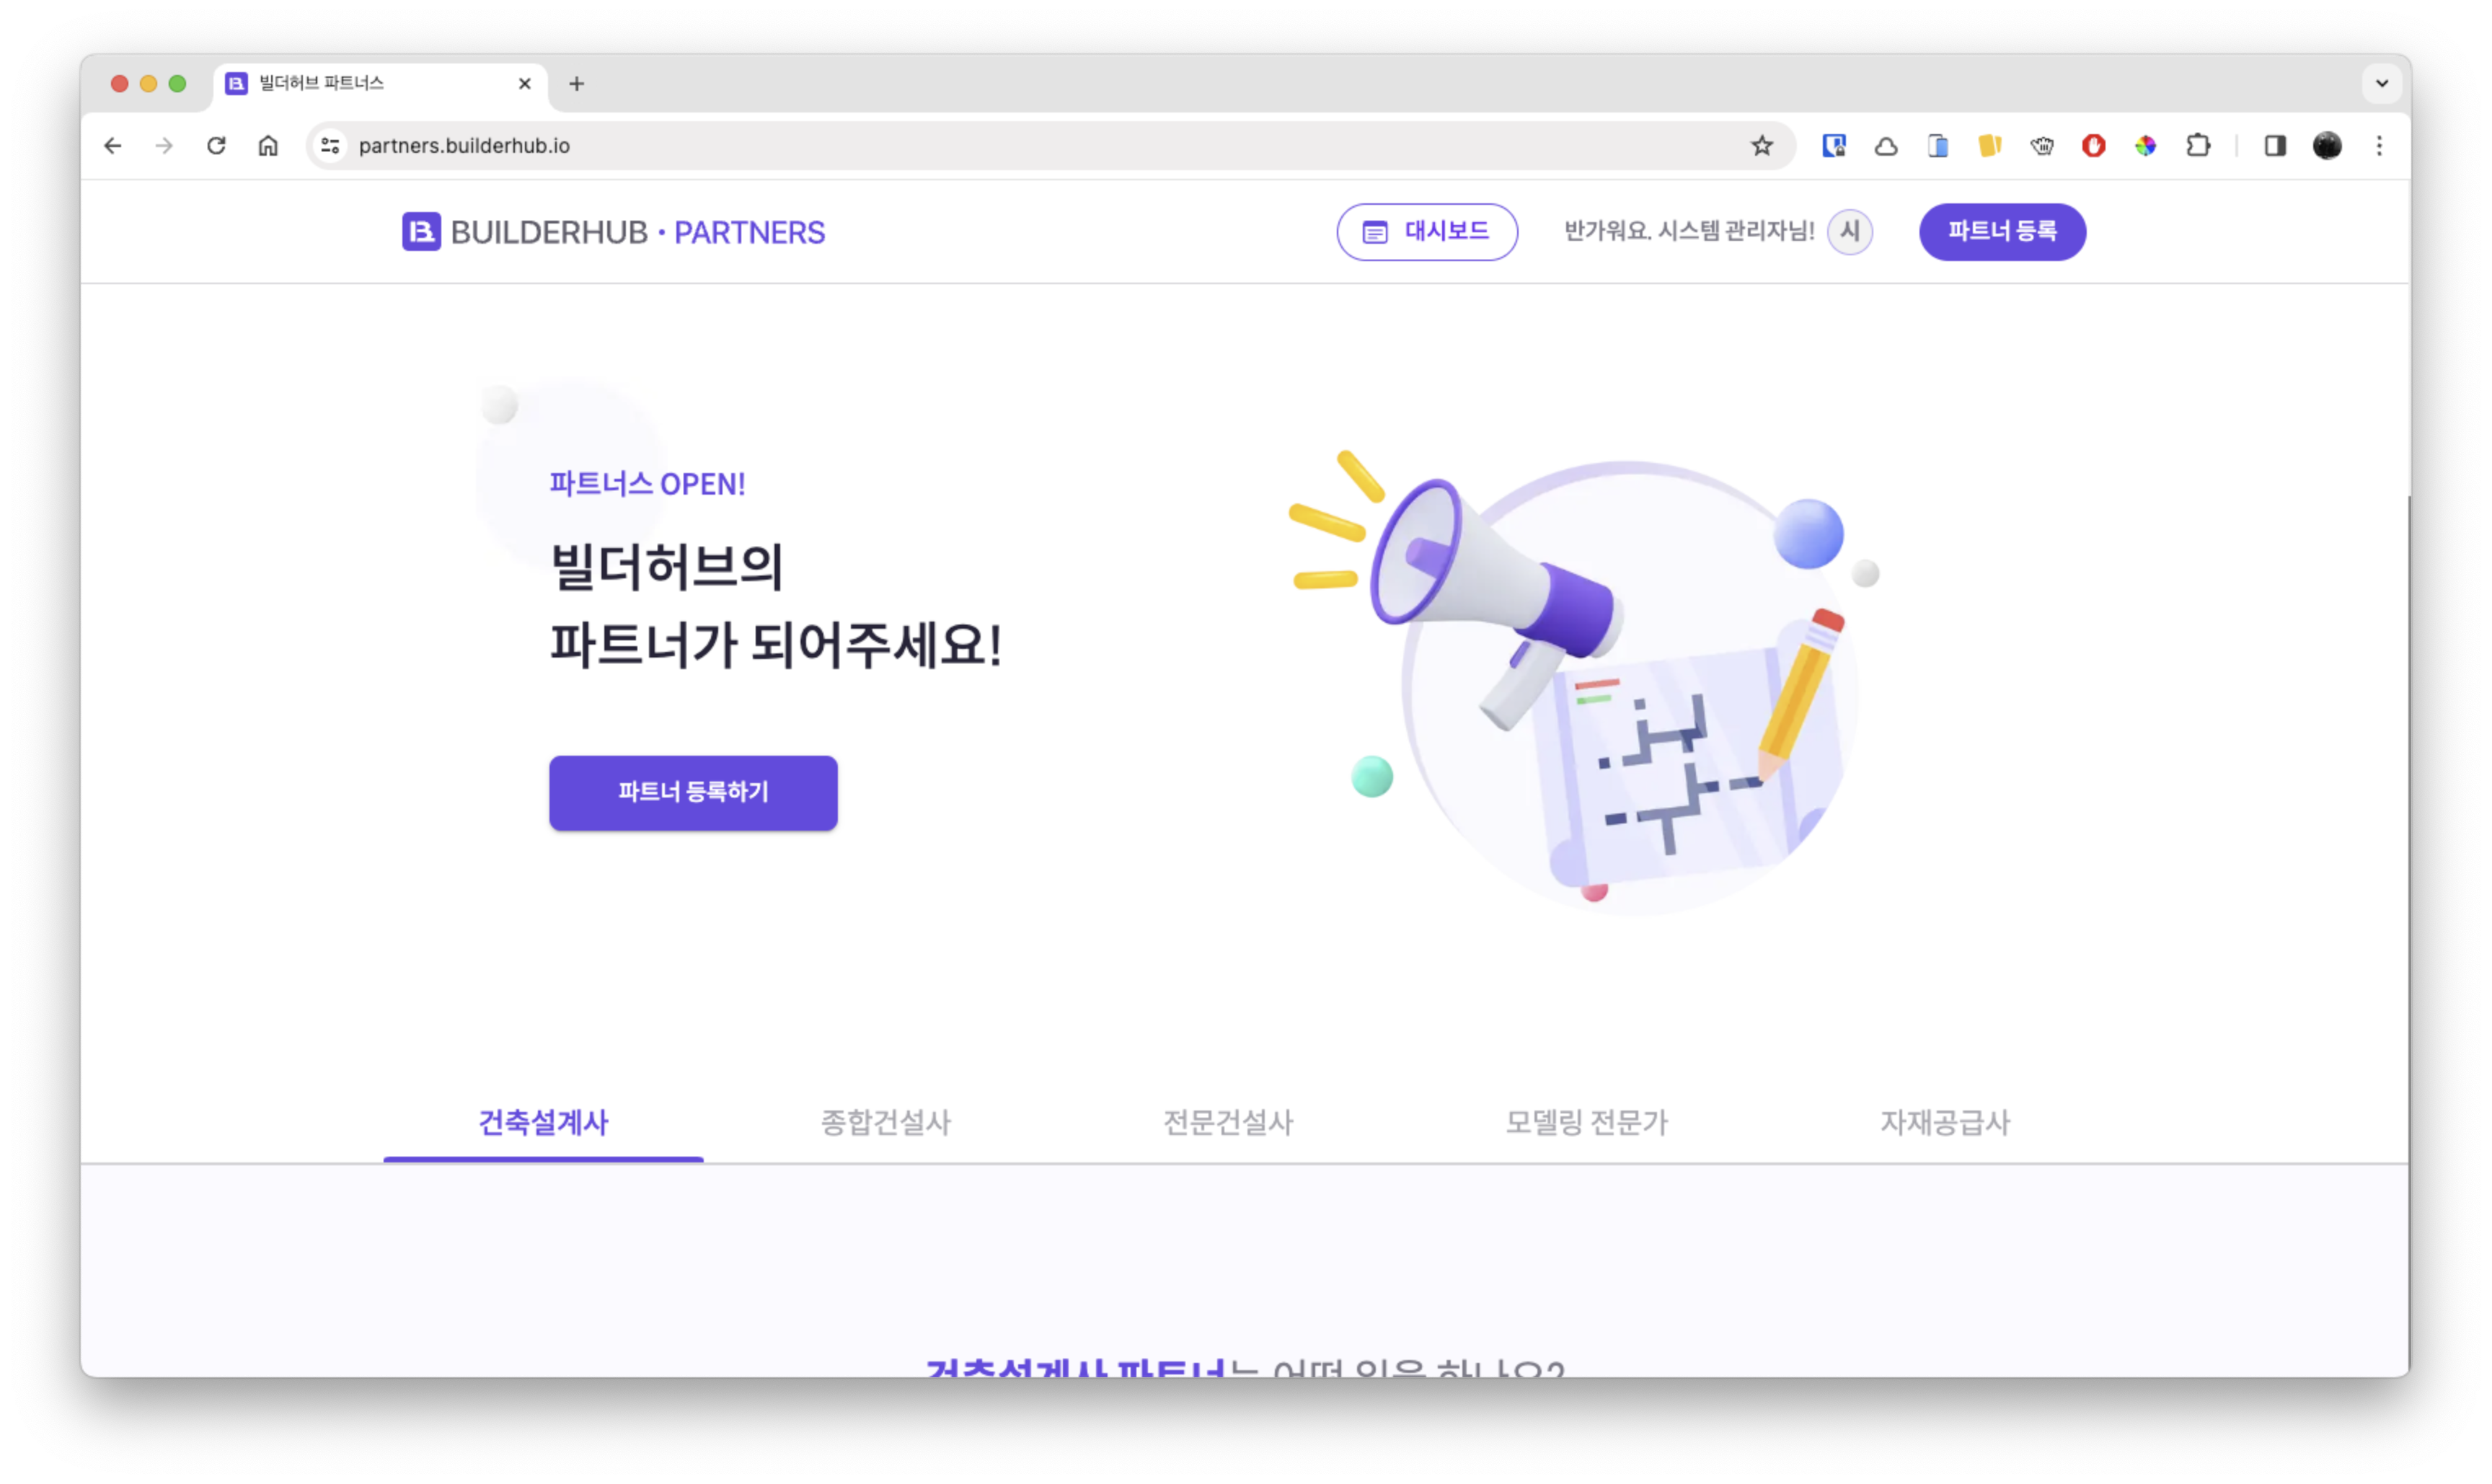
\includegraphics[width=0.35\textwidth]{images/builderhub-partners-main.png}
					            \caption*{Landing page}
				            }\qquad
				            \parbox{0.35\textwidth}{
					            \centering
					            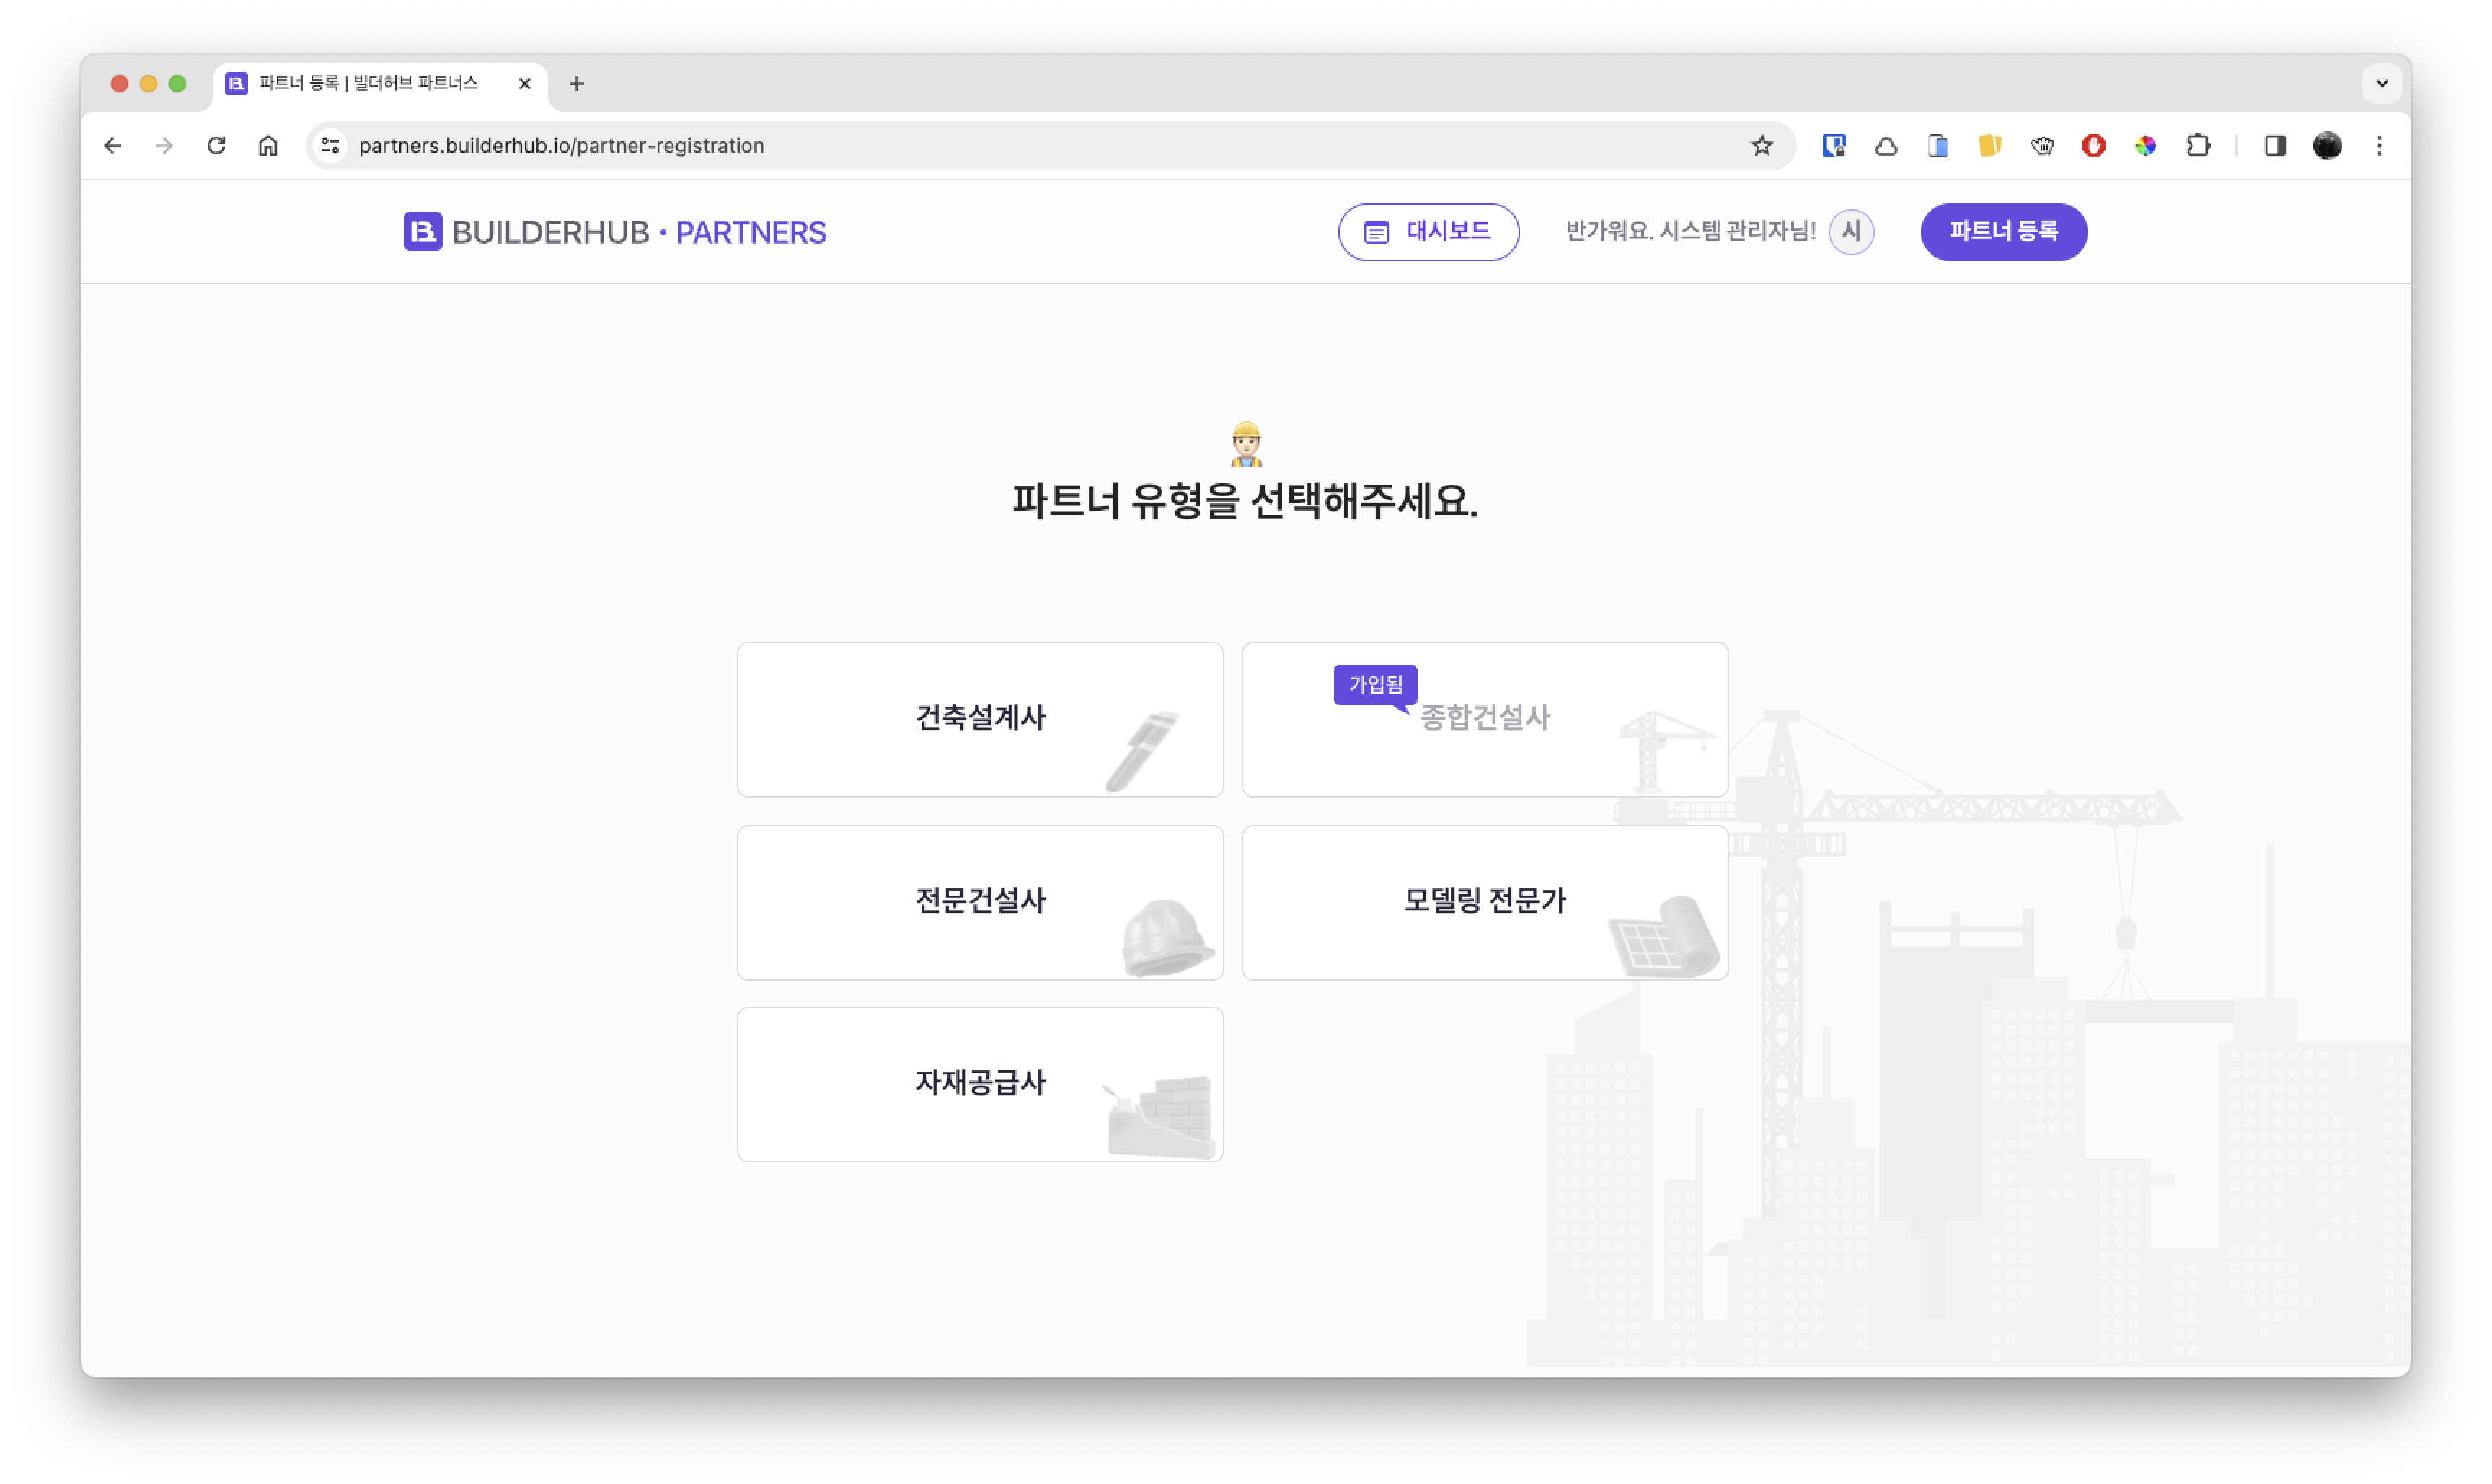
\includegraphics[width=0.35\textwidth]{images/builderhub-partners-join.png}
					            \caption*{Join partner}
				            }\qquad
				            \parbox{0.35\textwidth}{
					            \centering
					            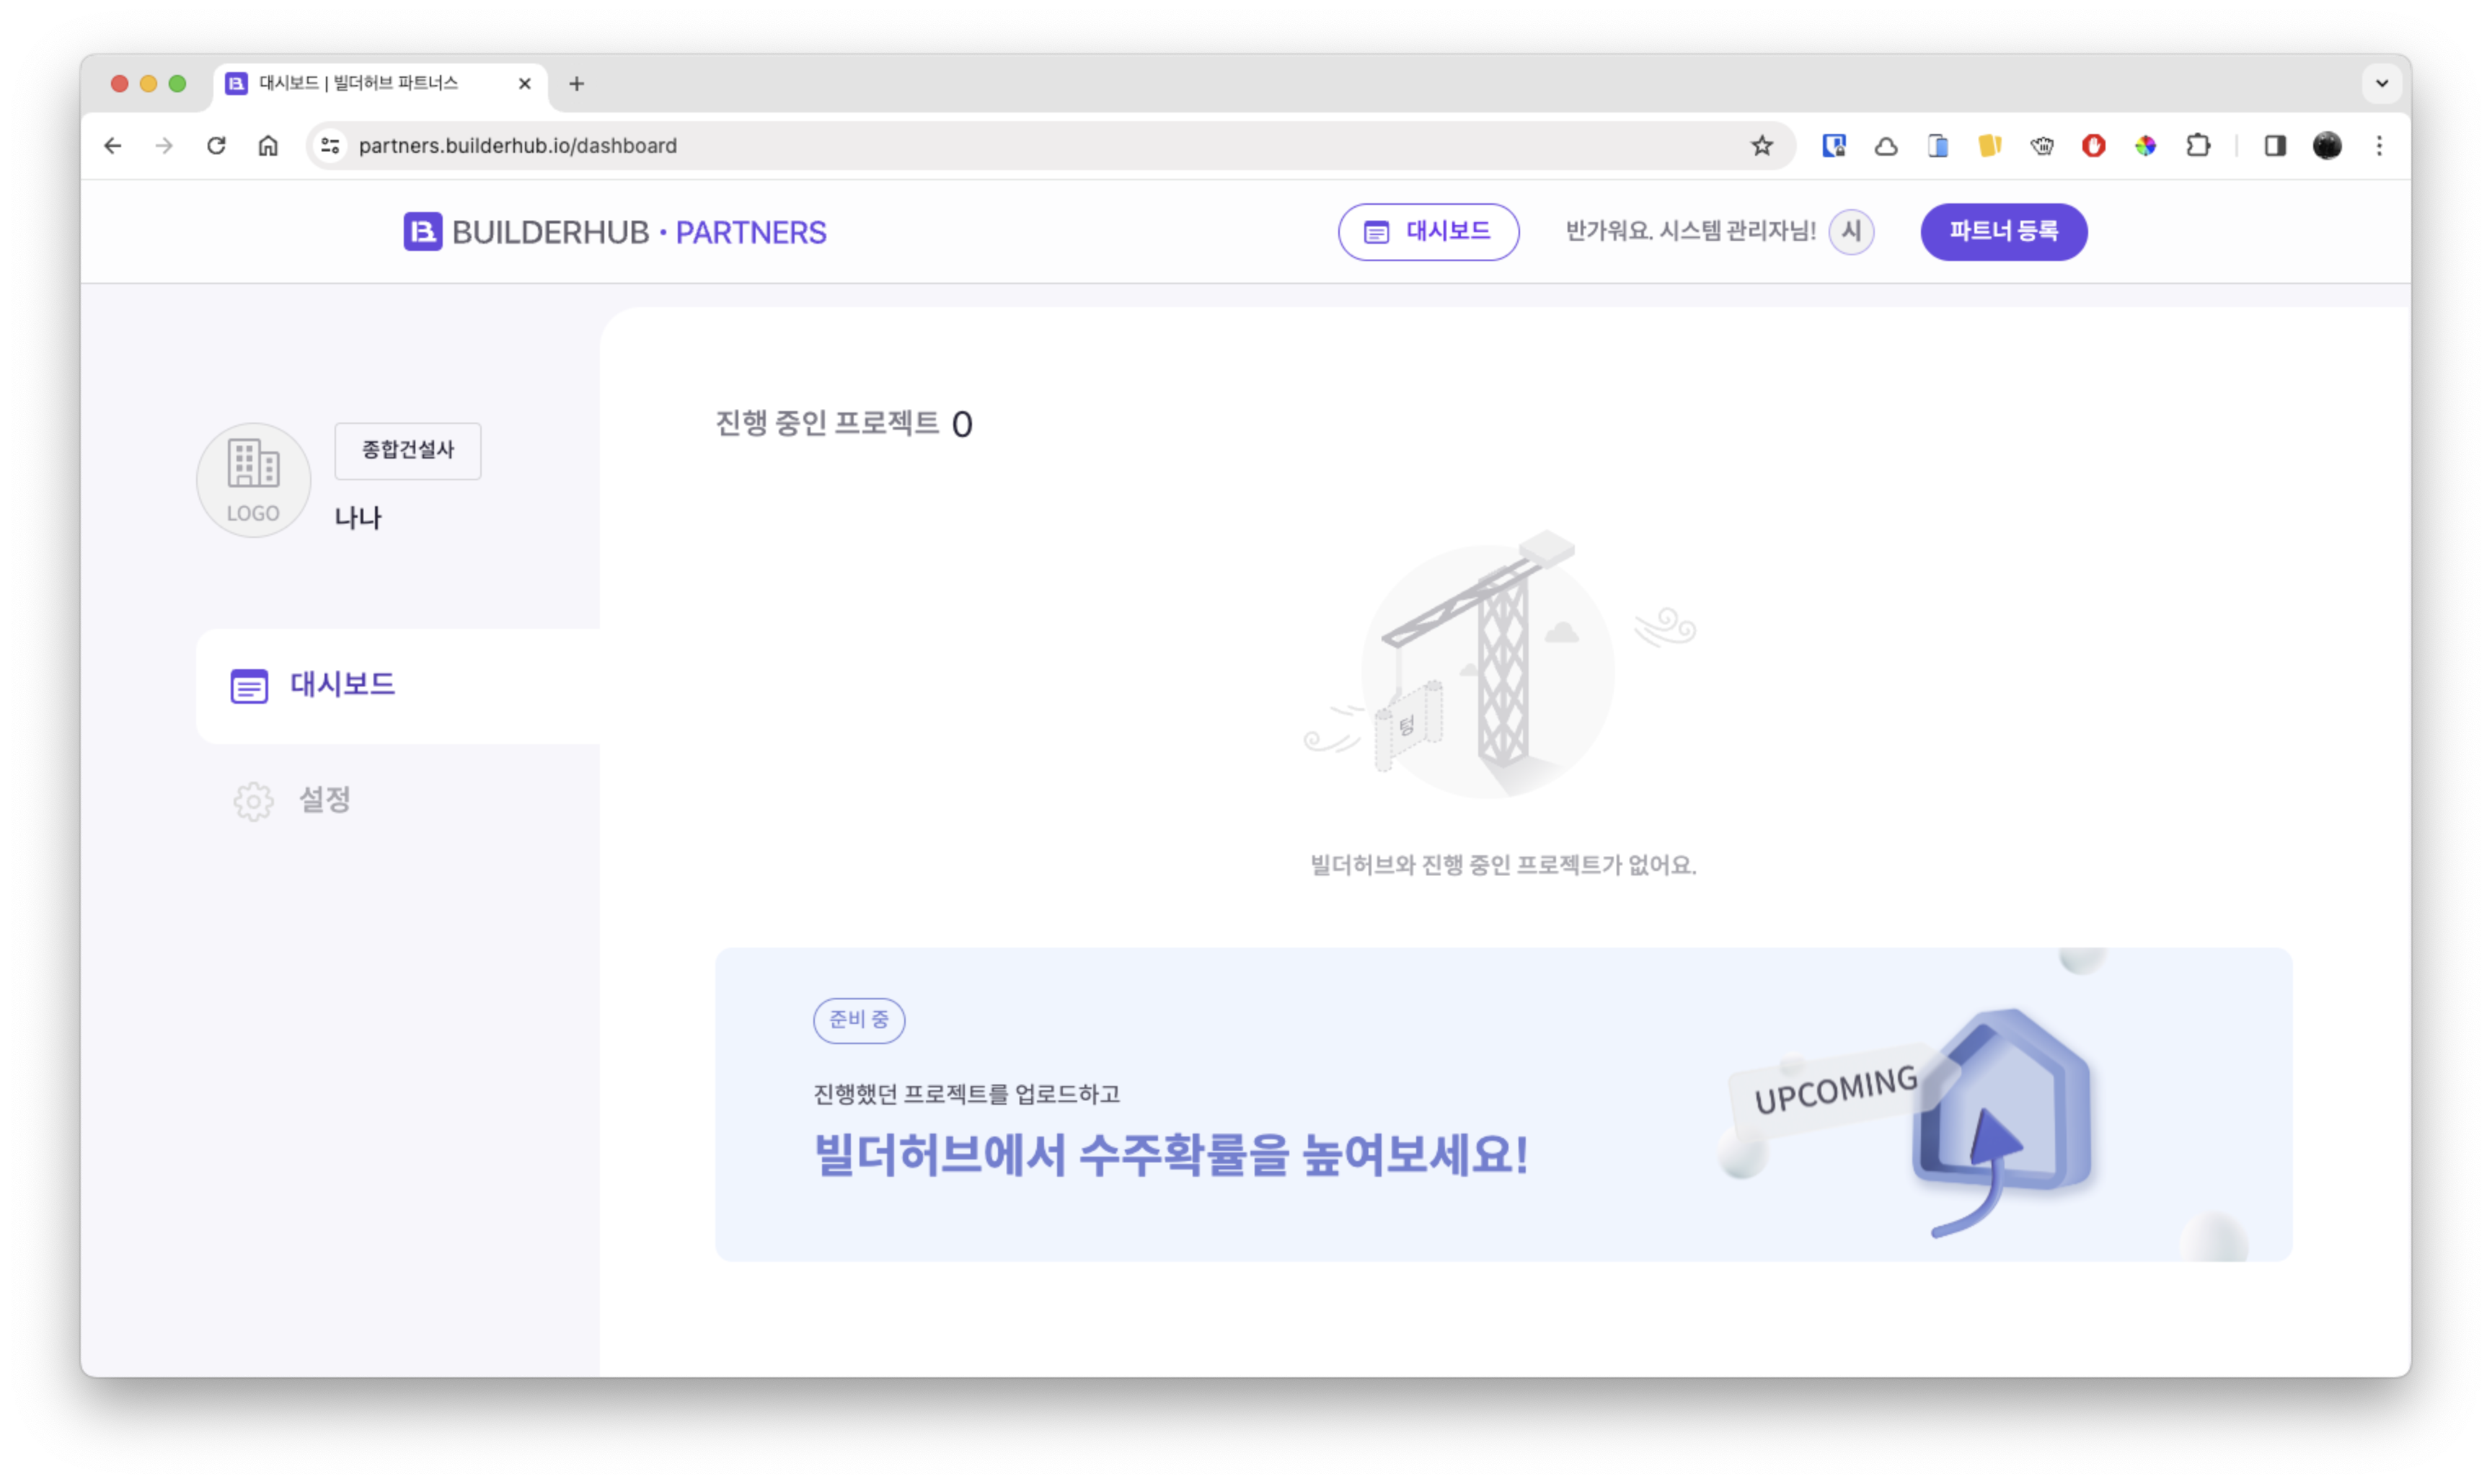
\includegraphics[width=0.35\textwidth]{images/builderhub-partners-dashboard.png}
					            \caption*{Dashboard}
				            }\qquad
				            \parbox{0.35\textwidth}{
					            \centering
					            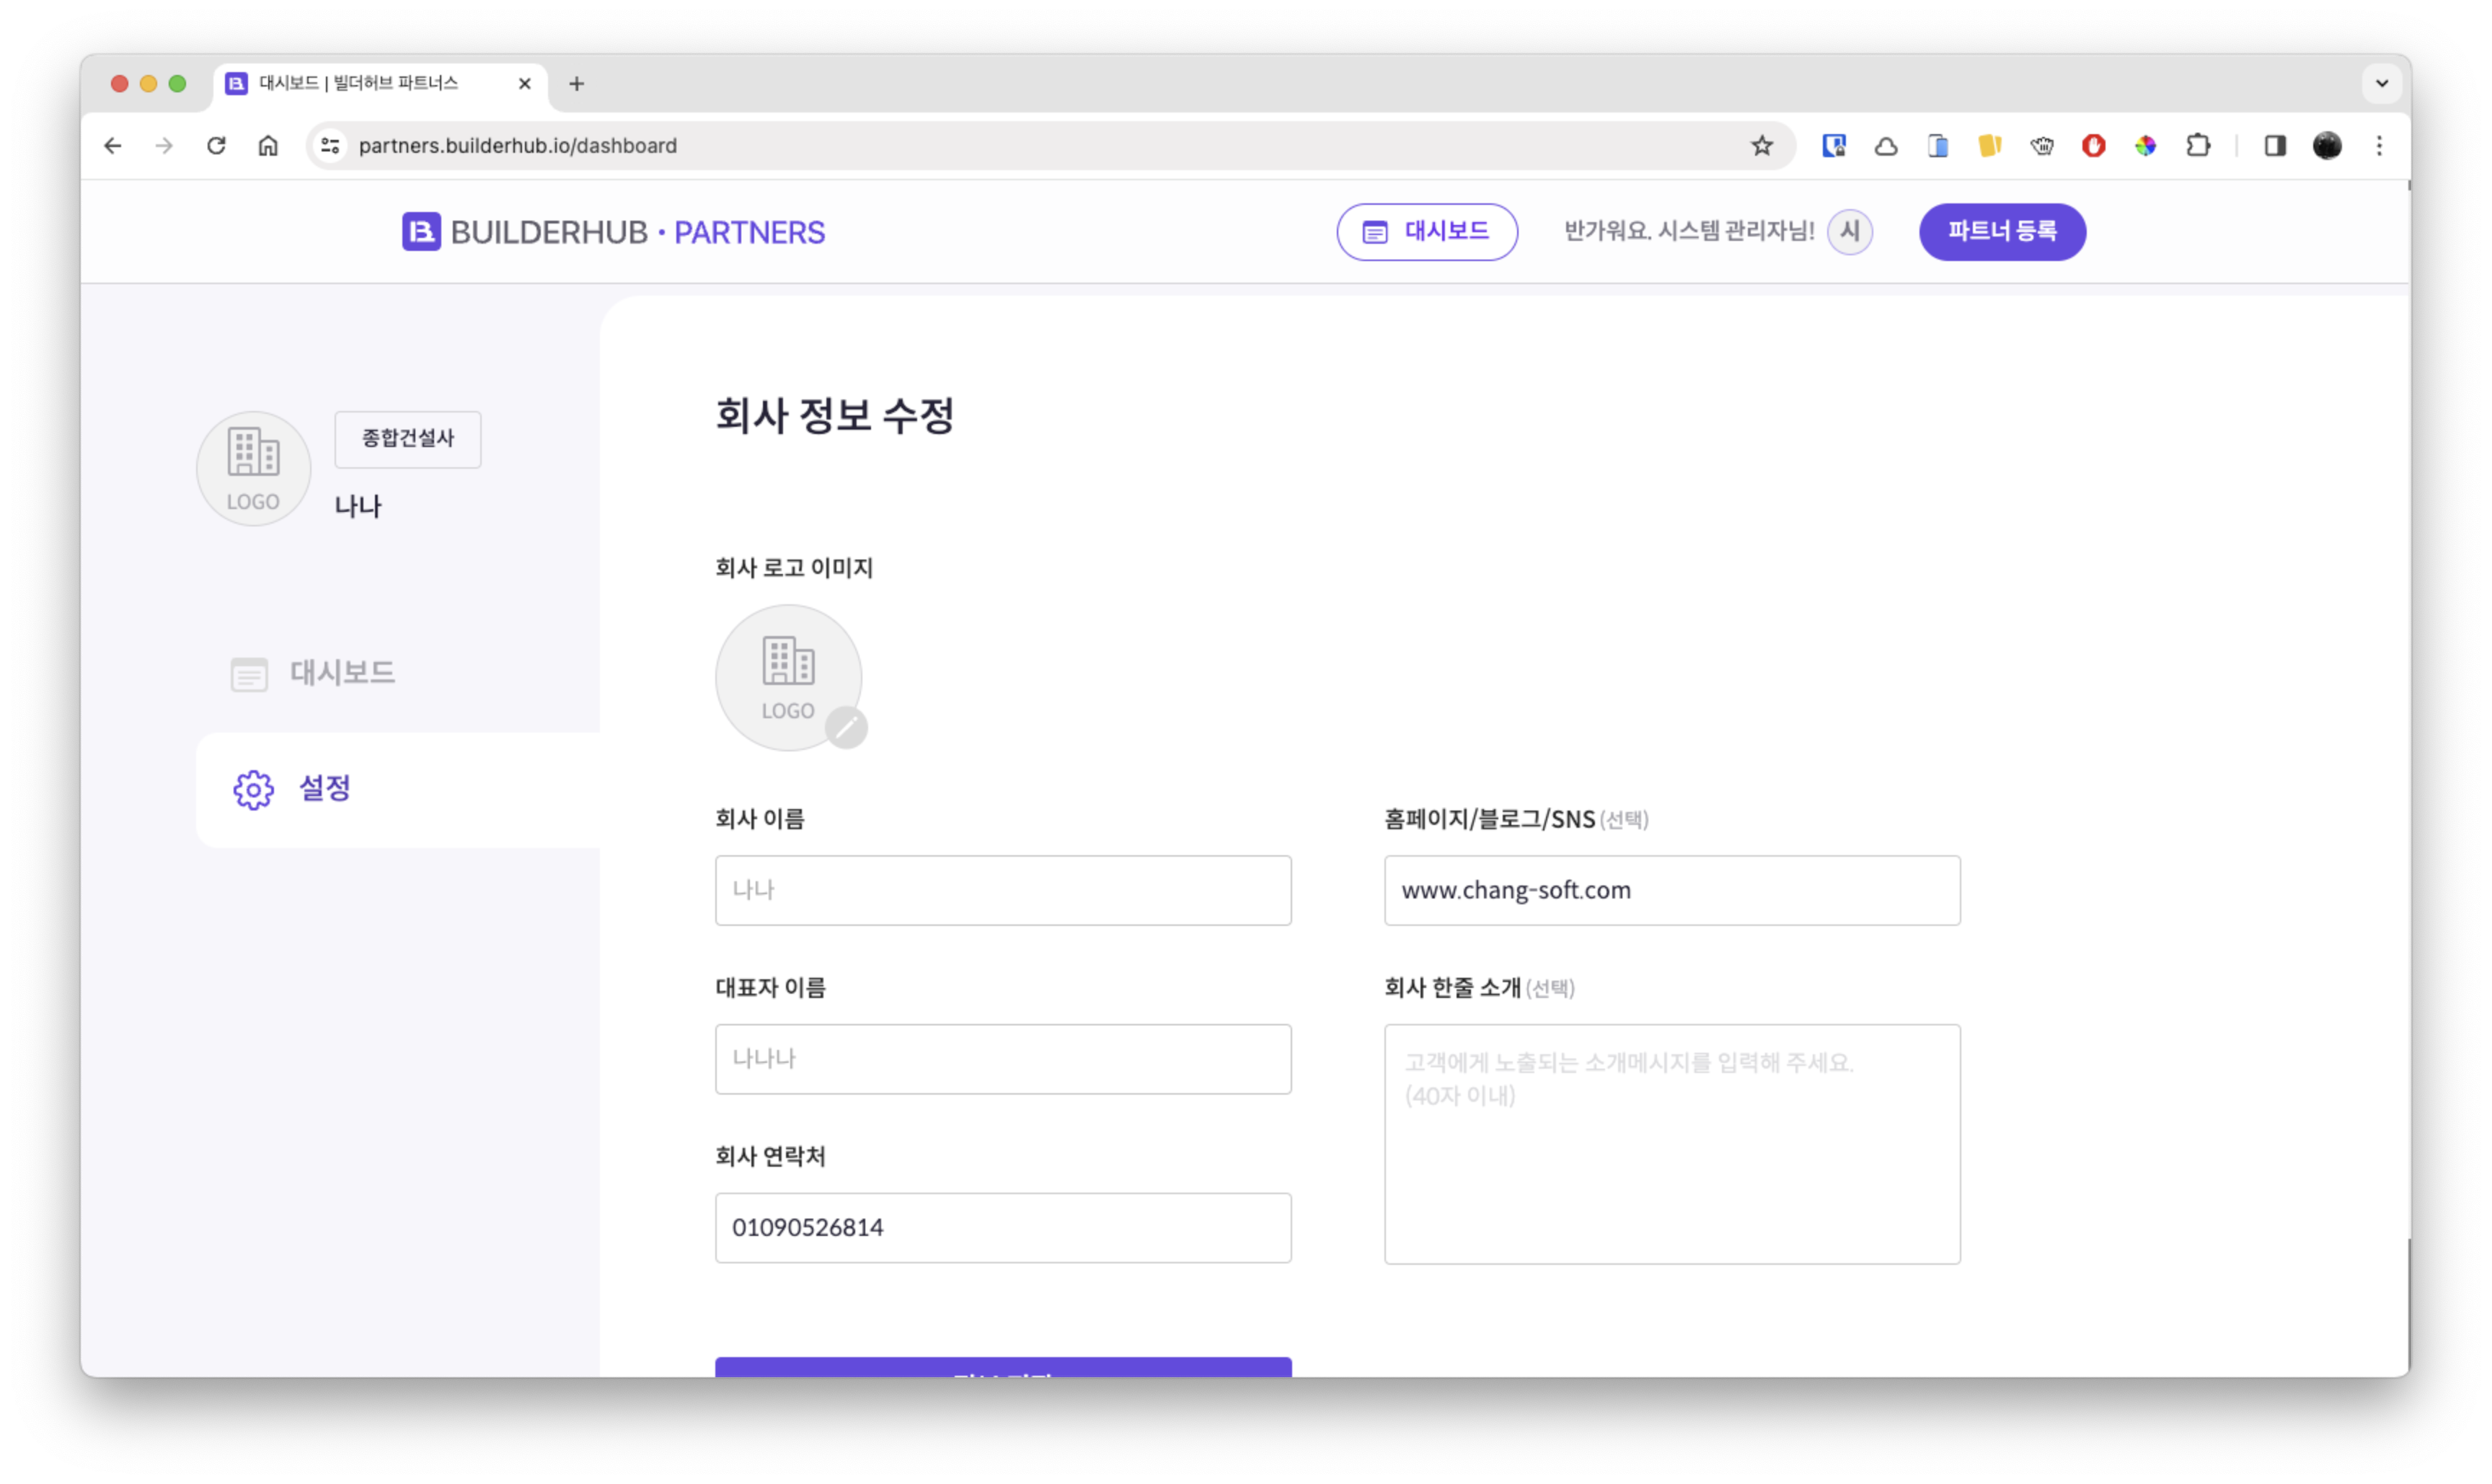
\includegraphics[width=0.35\textwidth]{images/builderhub-partners-edit.png}
					            \caption*{Edit profile}
				            }
			            \end{fullwidth}
		            \end{figure}
		      \item \textbf{\href{https://admin.prod.platform.builderhub.io/}{빌더허브 운영 어드민 (Back office)} 개발}
		            \begin{itemize}
			            \item 프로젝트 검수, 파트너 검수, 알림톡 송출, 결제 확인
			            \item 프로젝트 에셋 등록, 표준내역서 관리, 1:1문의 답변, FAQ 작성
		            \end{itemize}
		            \begin{figure}[!ht]
			            \begin{fullwidth}
				            \parbox{0.35\textwidth}{
					            \centering
					            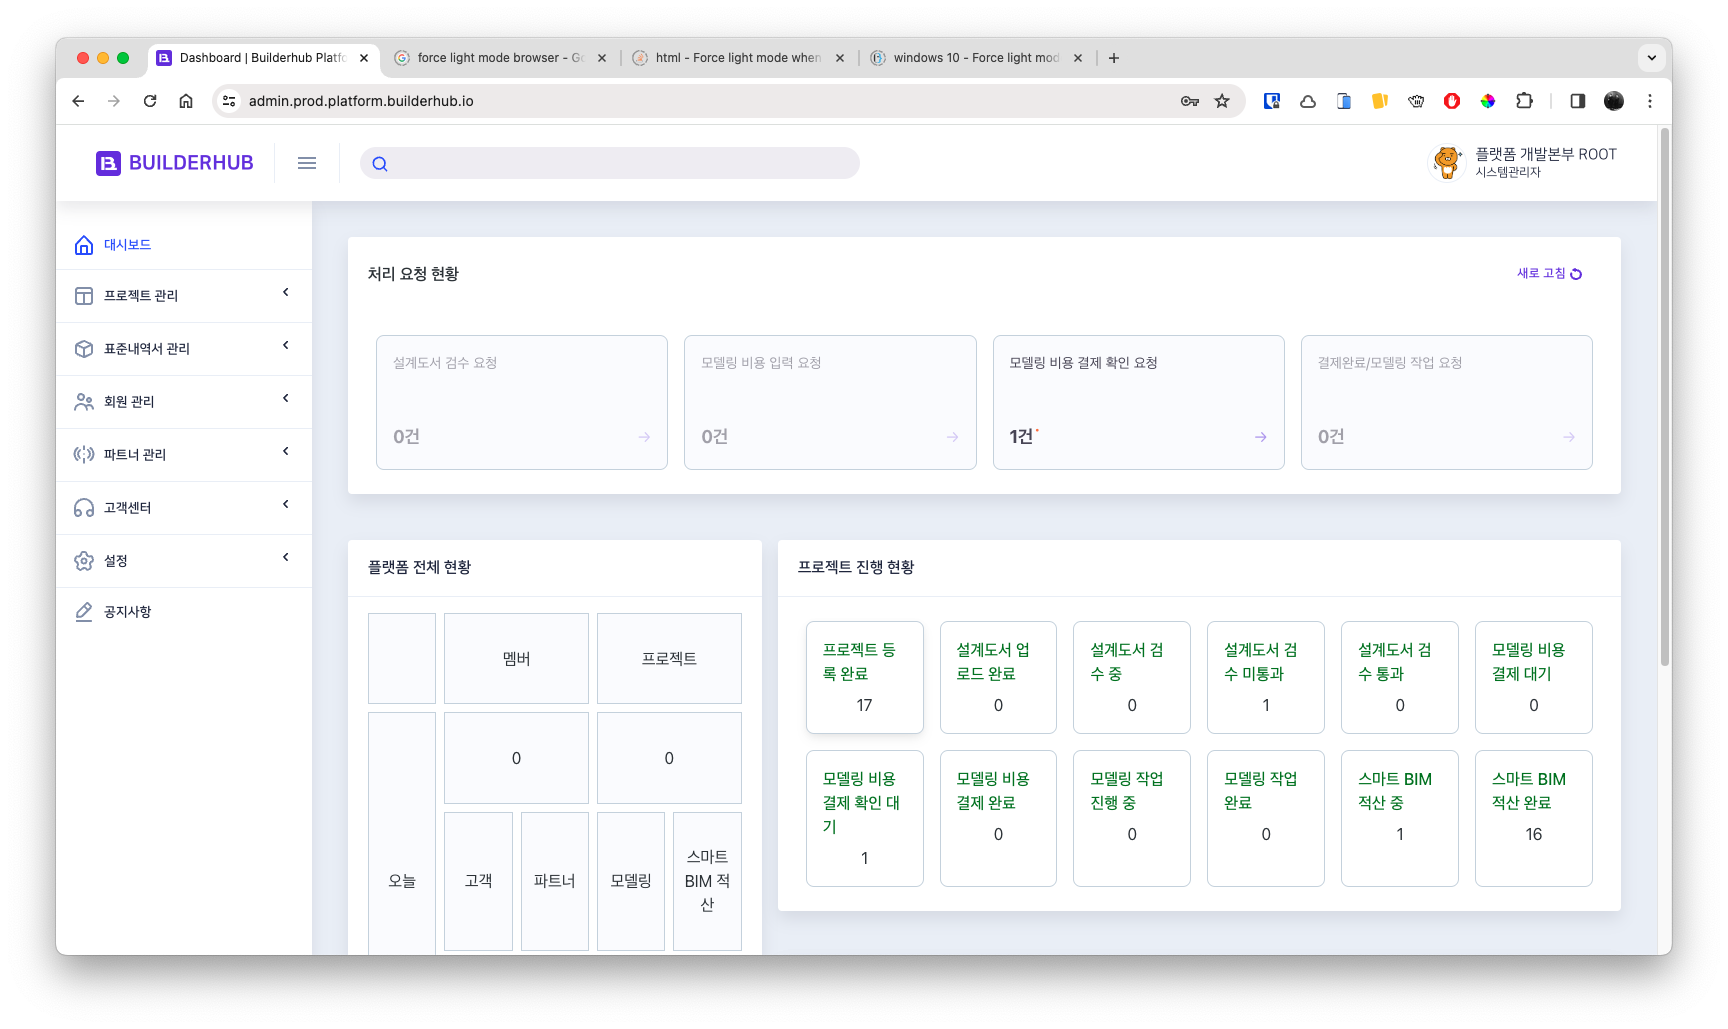
\includegraphics[width=0.35\textwidth]{images/builderhub-admin-dashboard.png}
					            \caption*{Dashboard}
				            }\qquad
				            \parbox{0.35\textwidth}{
					            \centering
					            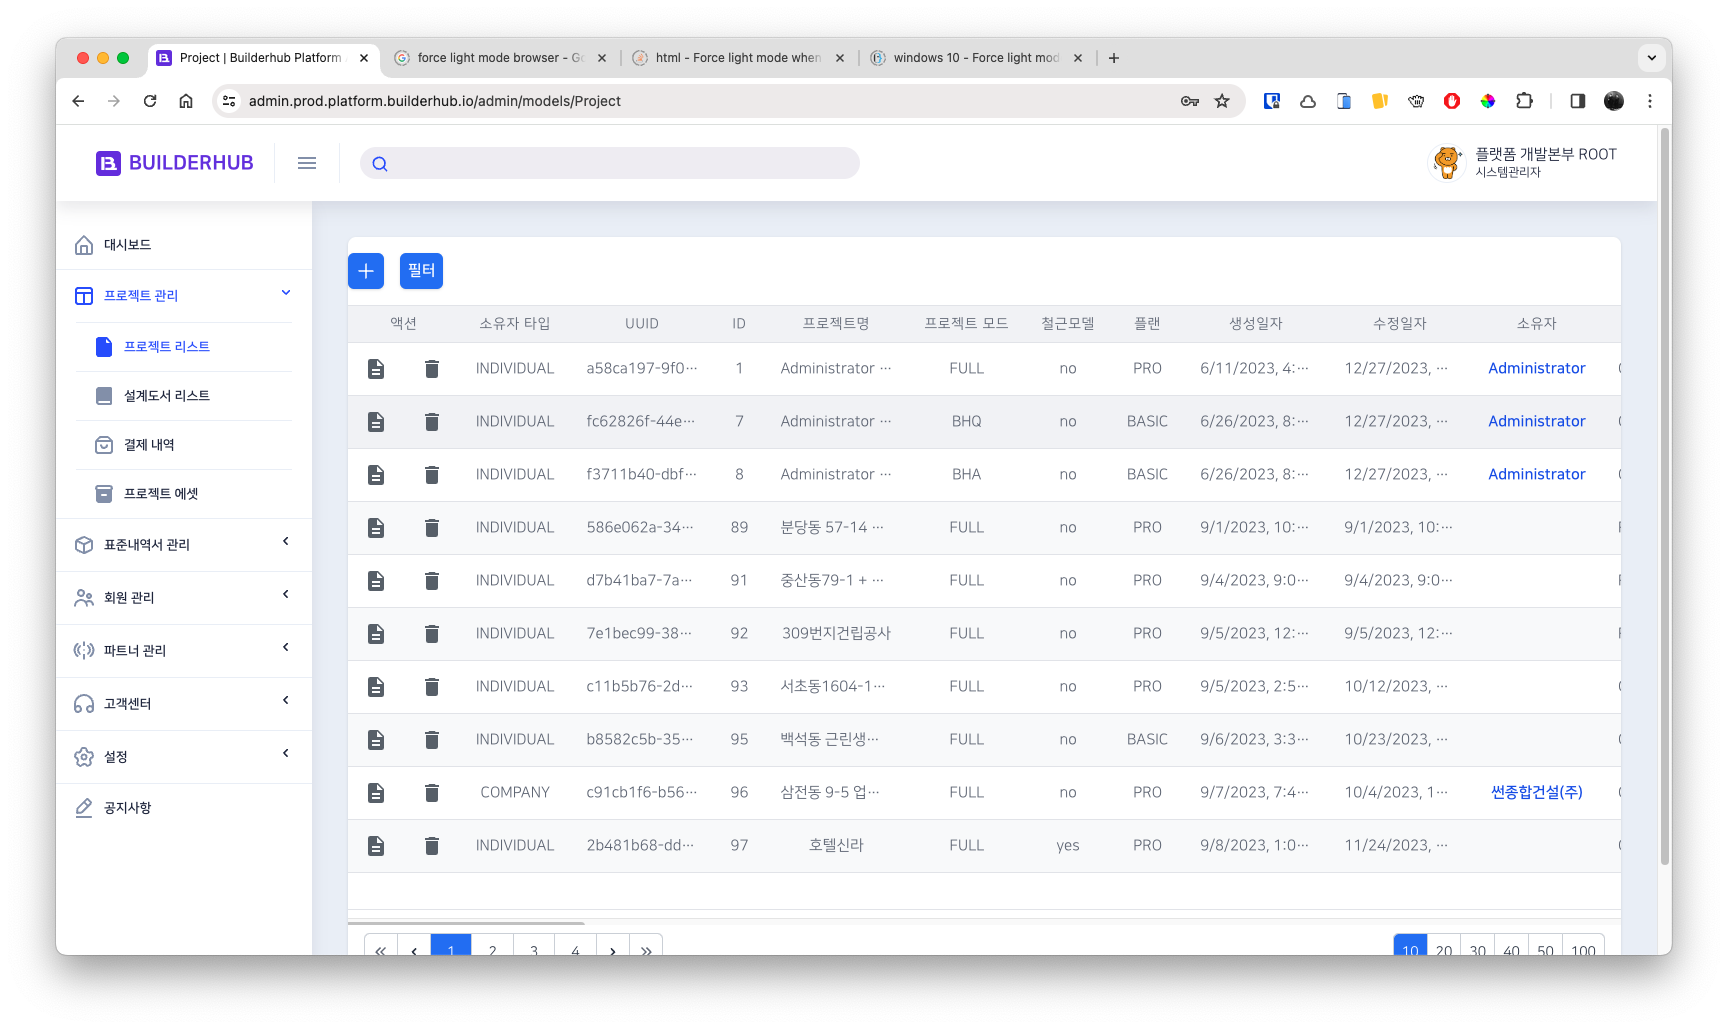
\includegraphics[width=0.35\textwidth]{images/builderhub-admin-project-list.png}
					            \caption*{Project list}
				            }\qquad
				            \parbox{0.35\textwidth}{
					            \centering
					            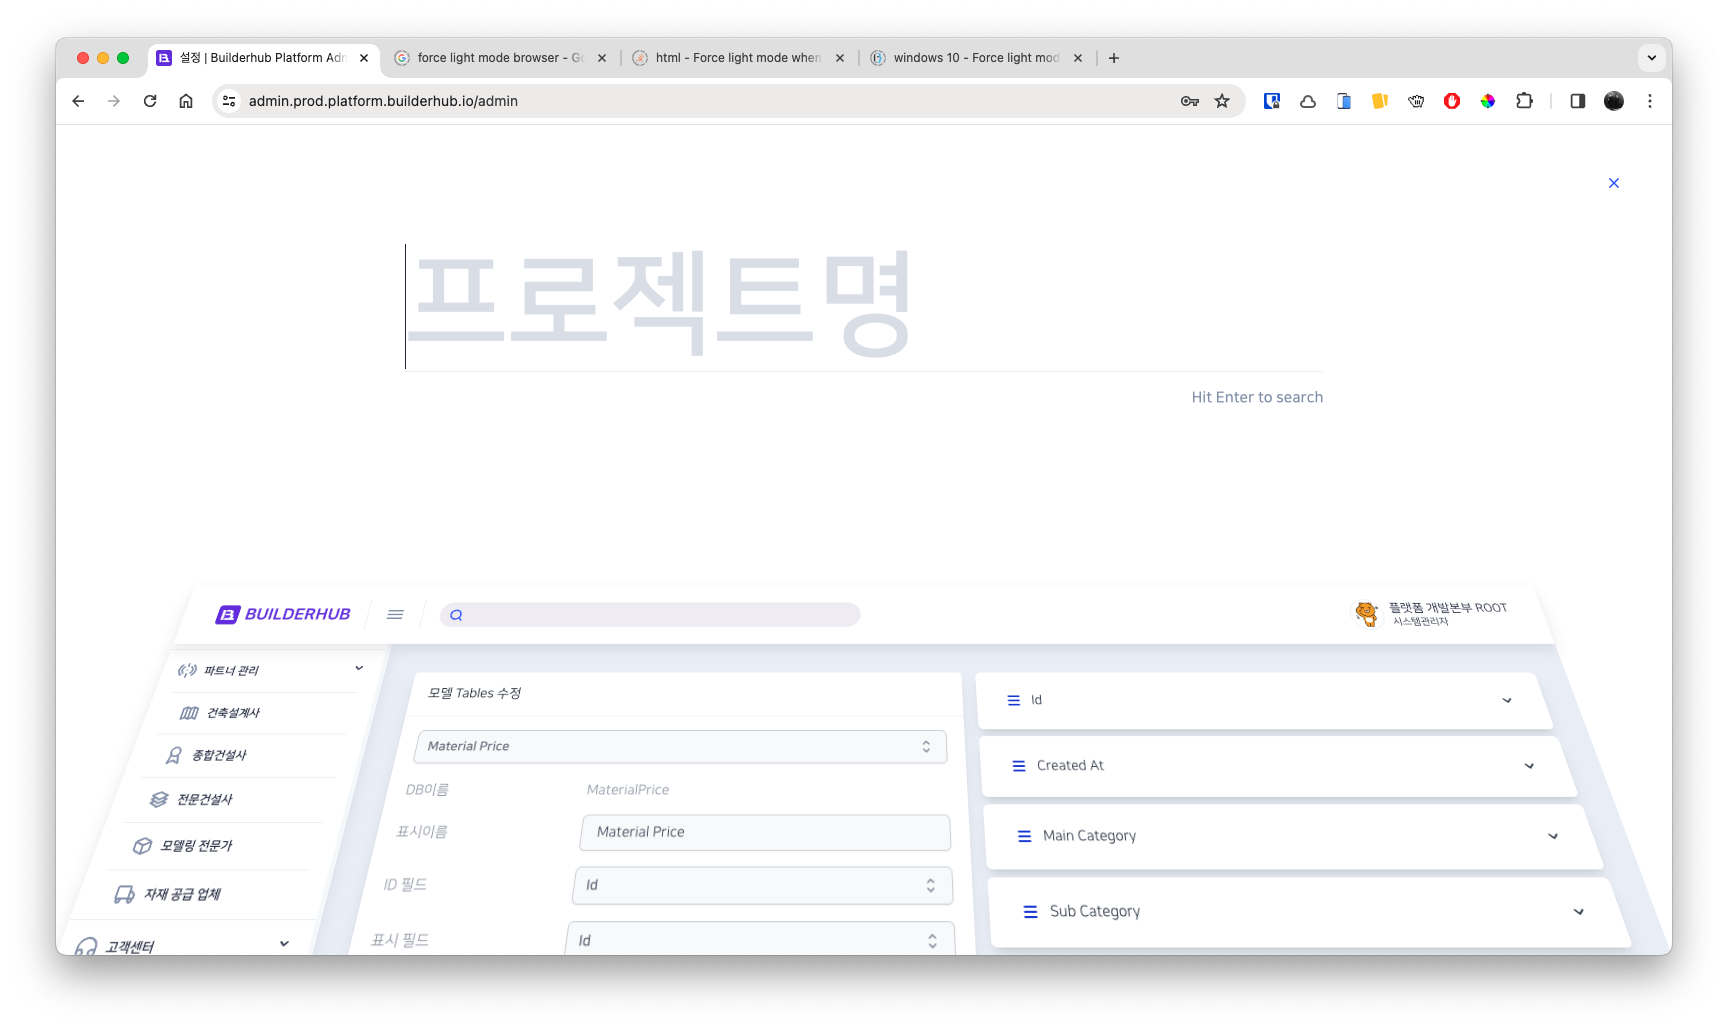
\includegraphics[width=0.35\textwidth]{images/builderhub-admin-project-search.png}
					            \caption*{Project search}
				            }\qquad
				            \parbox{0.35\textwidth}{
					            \centering
					            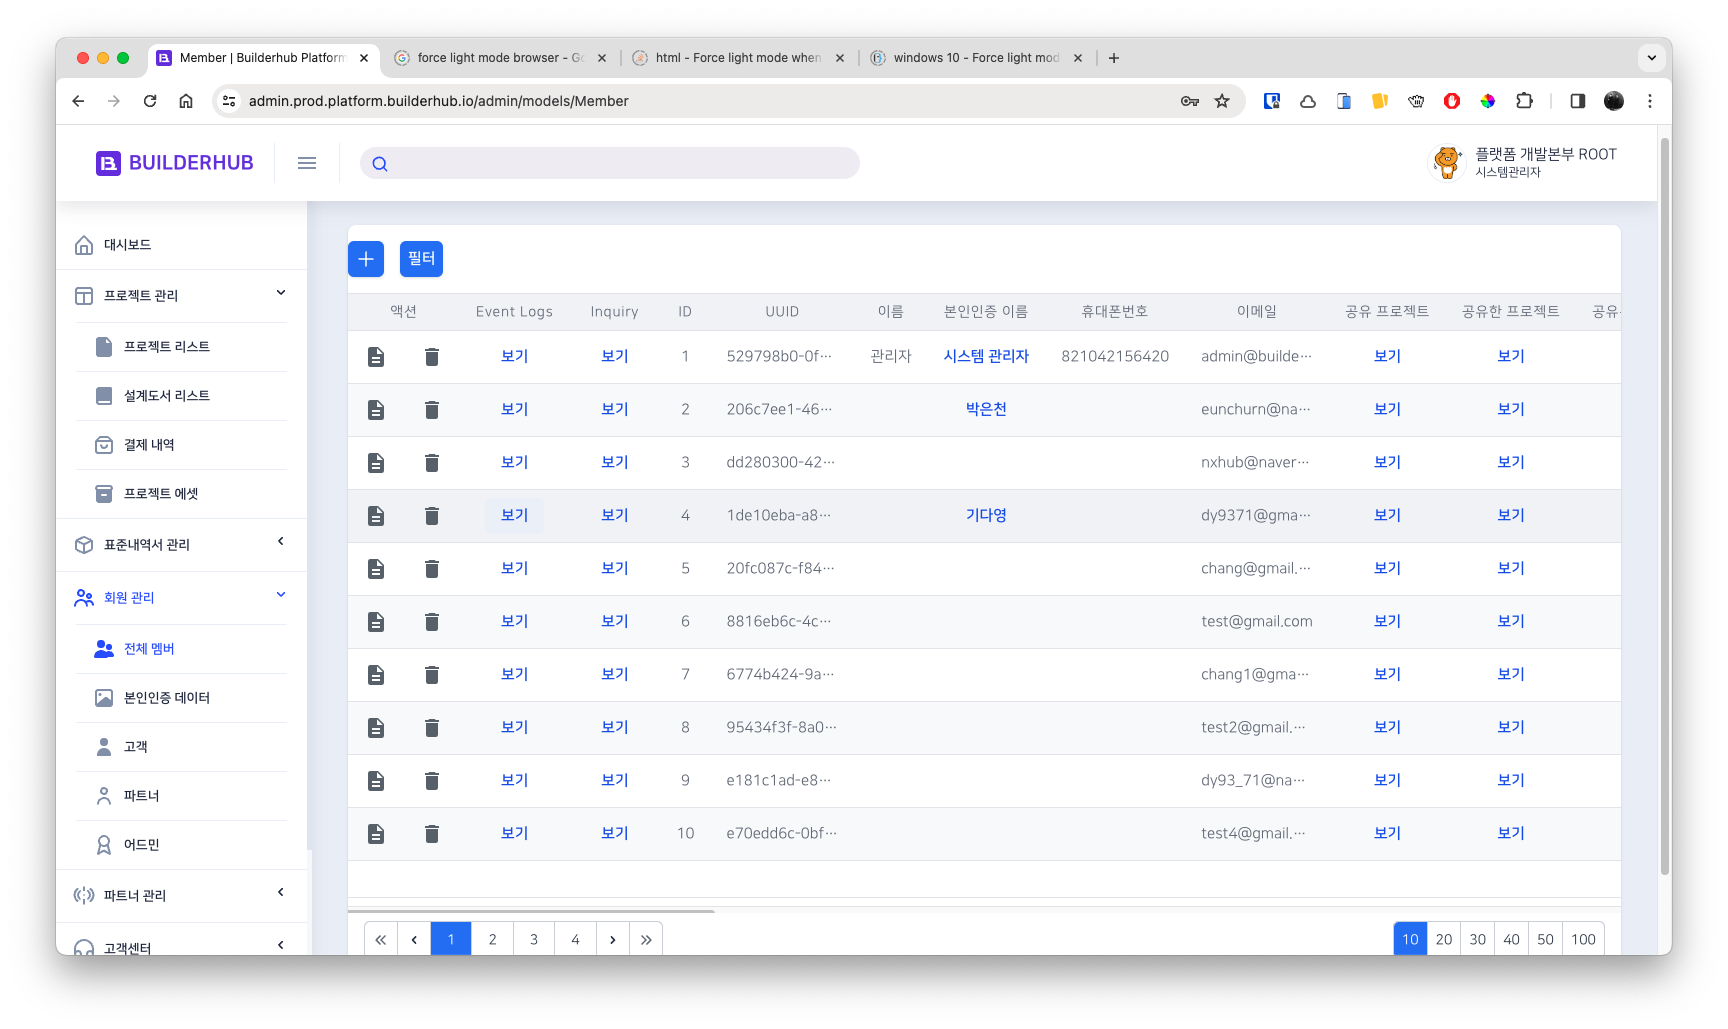
\includegraphics[width=0.35\textwidth]{images/builderhub-admin-member-list.png}
					            \caption*{Member list}
				            }
				            \parbox{0.35\textwidth}{
					            \centering
					            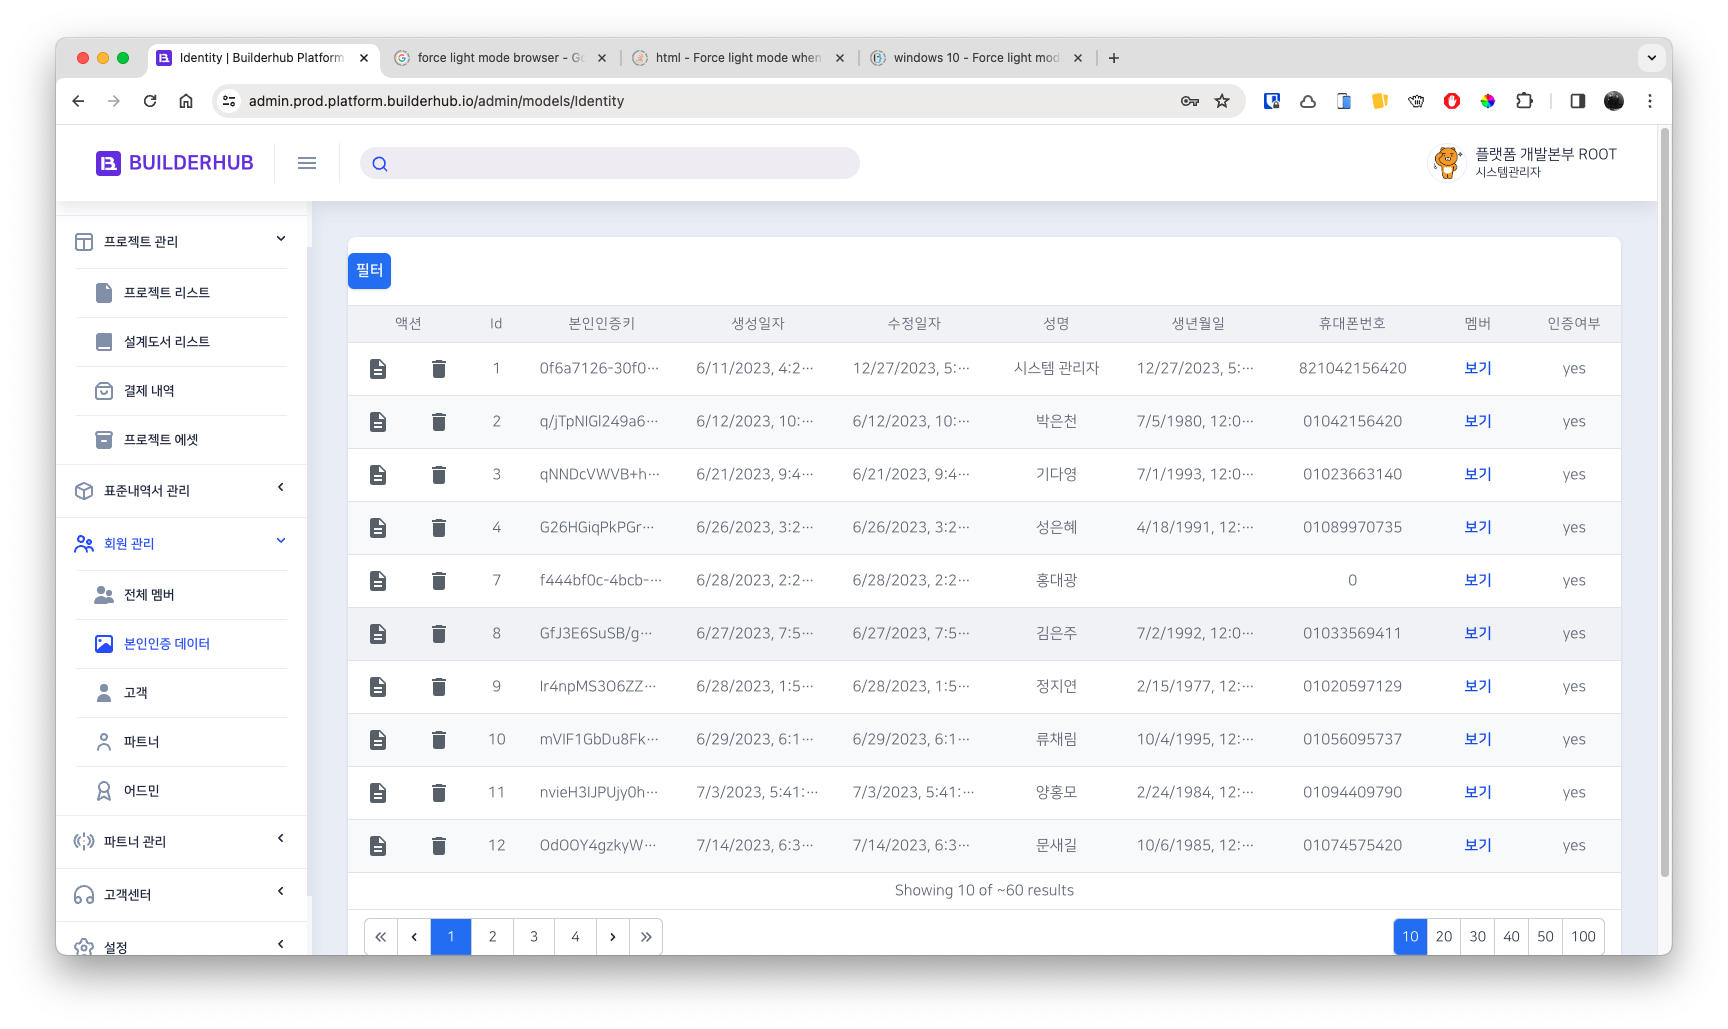
\includegraphics[width=0.35\textwidth]{images/builderhub-admin-member-identity.png}
					            \caption*{Member identity}
				            }\qquad
				            \parbox{0.35\textwidth}{
					            \centering
					            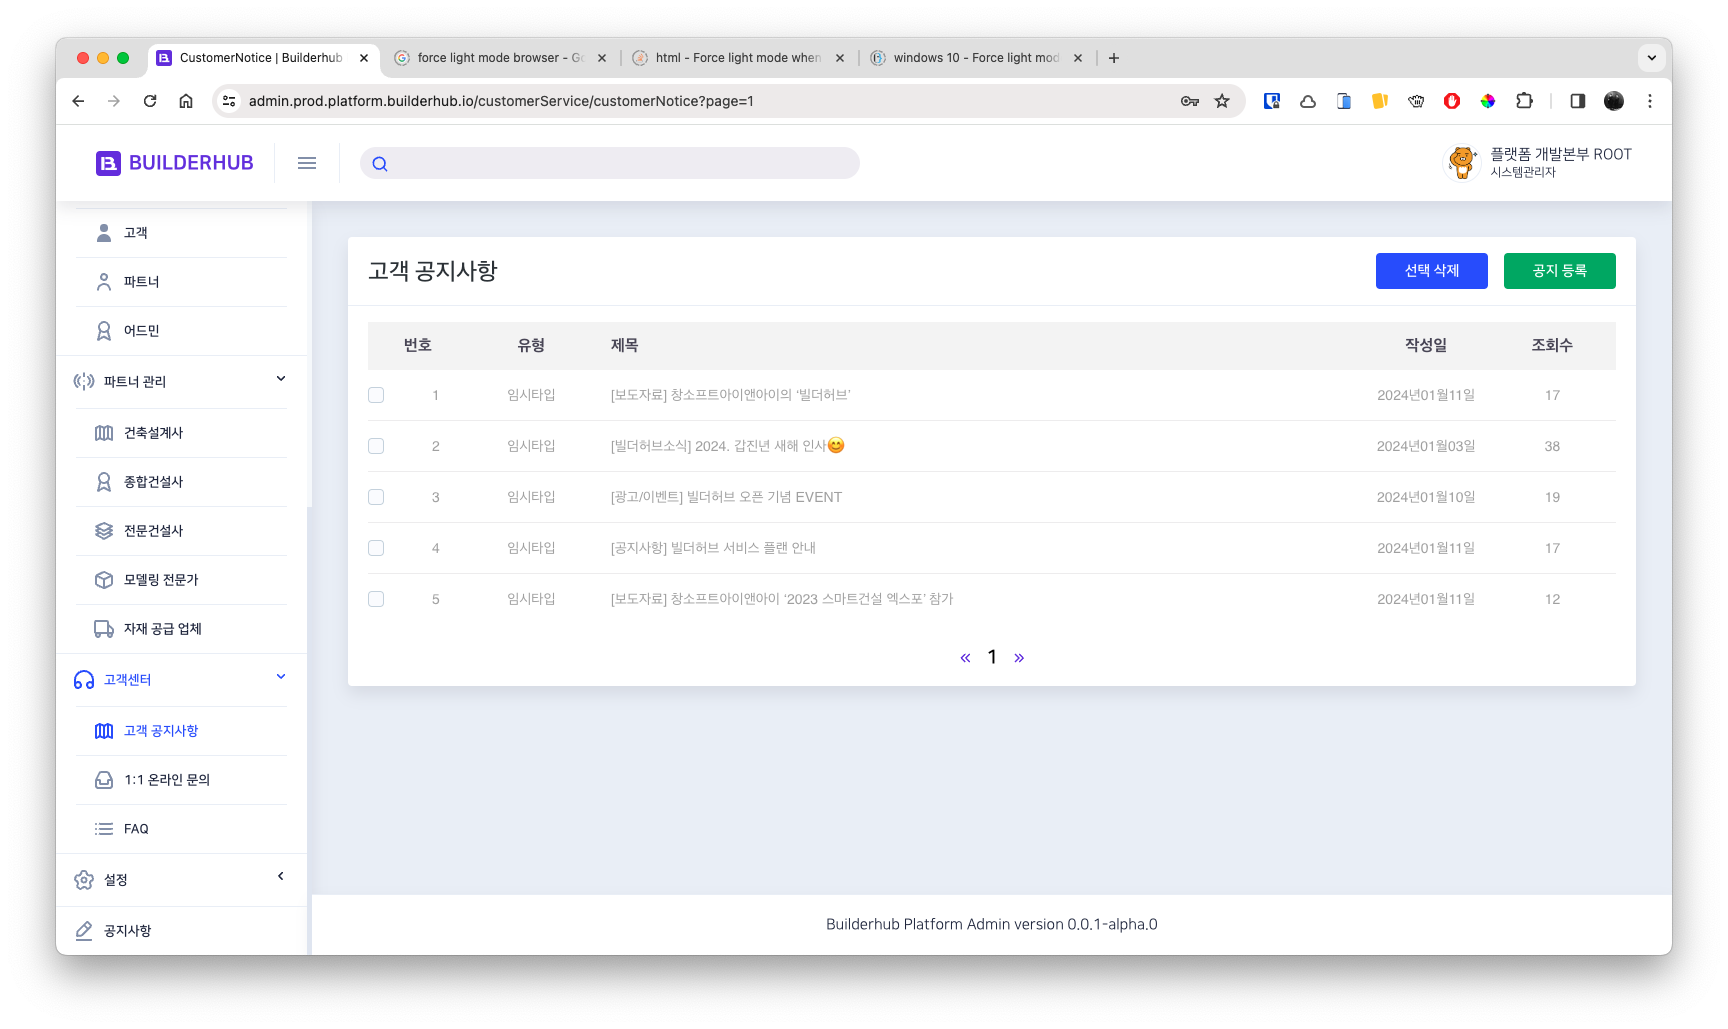
\includegraphics[width=0.35\textwidth]{images/builderhub-admin-notice.png}
					            \caption*{Notice}
				            }\qquad
				            \parbox{0.35\textwidth}{
					            \centering
					            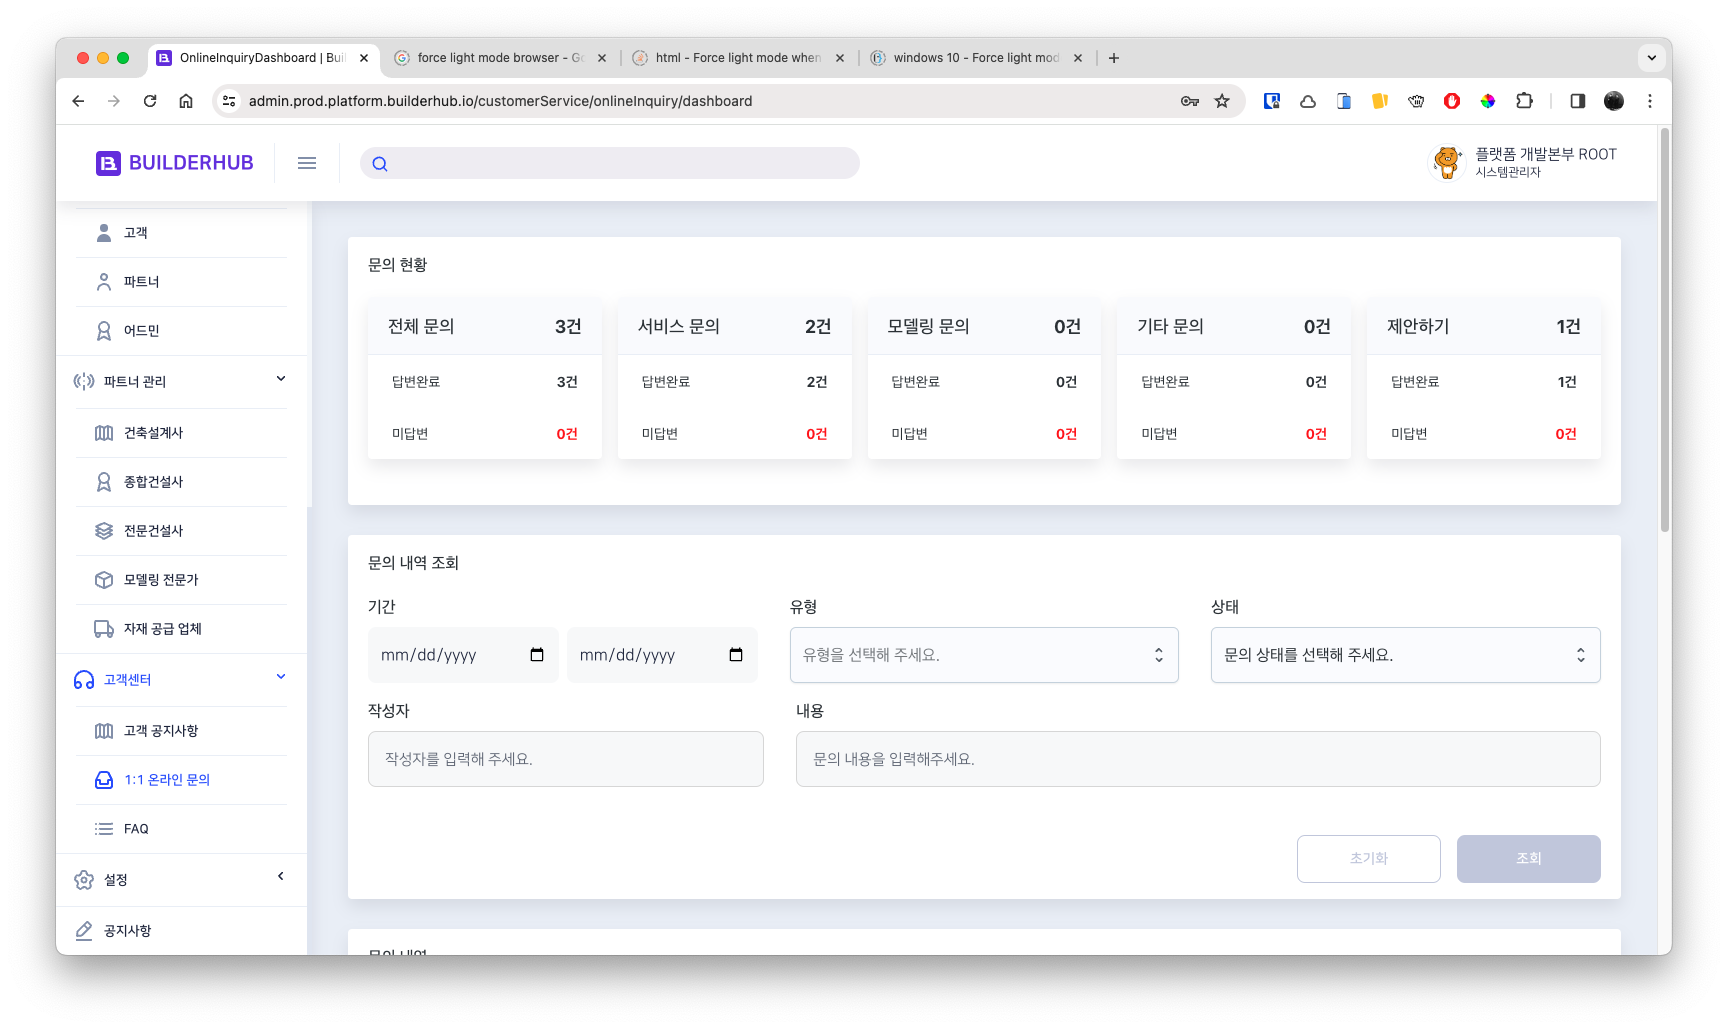
\includegraphics[width=0.35\textwidth]{images/builderhub-admin-one-to-one-qa.png}
					            \caption*{1:1 문의}
				            }\qquad
				            \parbox{0.35\textwidth}{
					            \centering
					            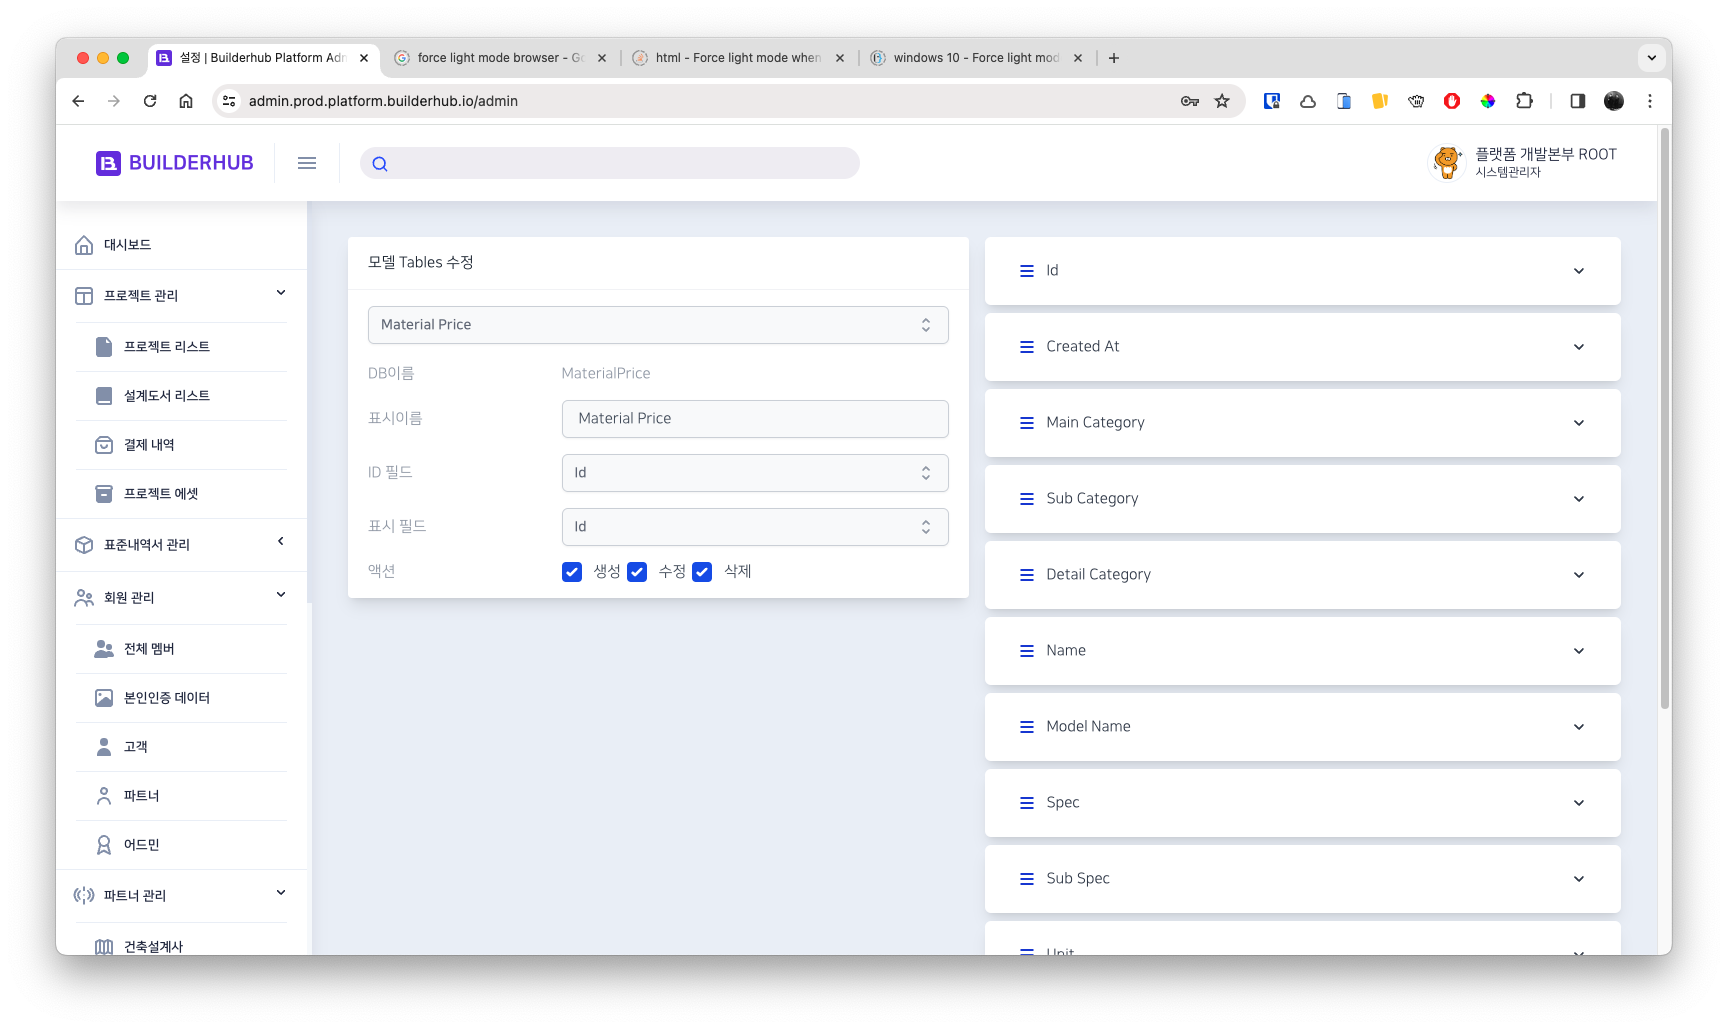
\includegraphics[width=0.35\textwidth]{images/builderhub-admin-settings.png}
					            \caption*{Settings}
				            }
			            \end{fullwidth}
		            \end{figure}
		      \item \textbf{플랫폼 컨버터 개발}
		            \begin{itemize}
			            \item 솔루션 데이터 프리프로세싱, 디폴트 값 추가
			            \item 비내역화 데이터 계산 및 추가, 표준내역서 매핑, 공사비 데이터 매핑 및 공사비 산출
			            \item 솔루션 BIM 모델데이터 업로드 및 변환
			            \item 개발 스택: TypeScript, NodeJS, ElectronJS, NextJS(Nextron), Default data and Validator(AJV), CSV Parser(papaparse)
		            \end{itemize}
		            \begin{figure}[!ht]
			            \begin{fullwidth}
				            \parbox{0.45\textwidth}{
					            \centering
					            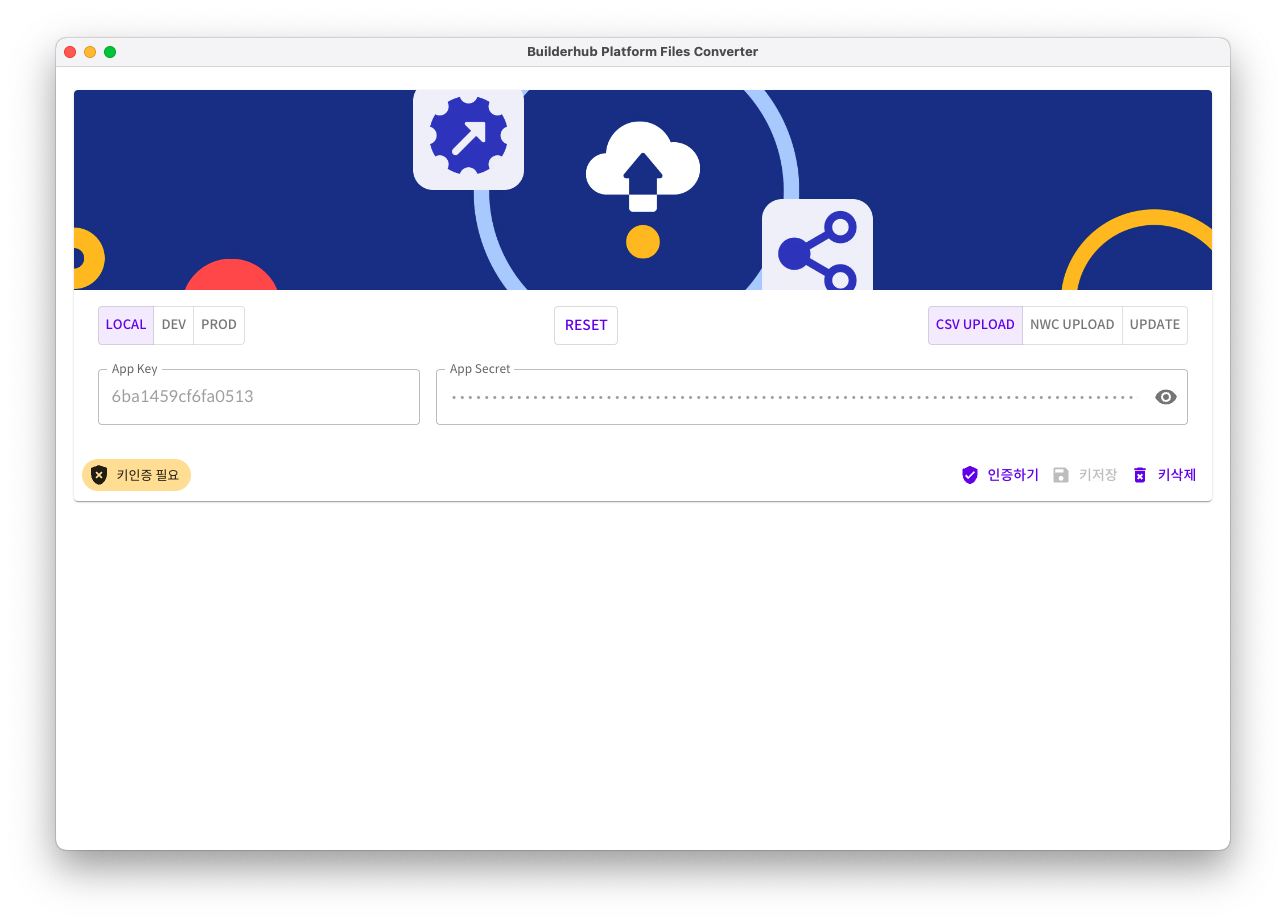
\includegraphics[width=0.28\textwidth]{images/builderhub-converter-main.png}
					            \caption*{Main}
				            }\qquad
				            \parbox{0.45\textwidth}{
					            \centering
					            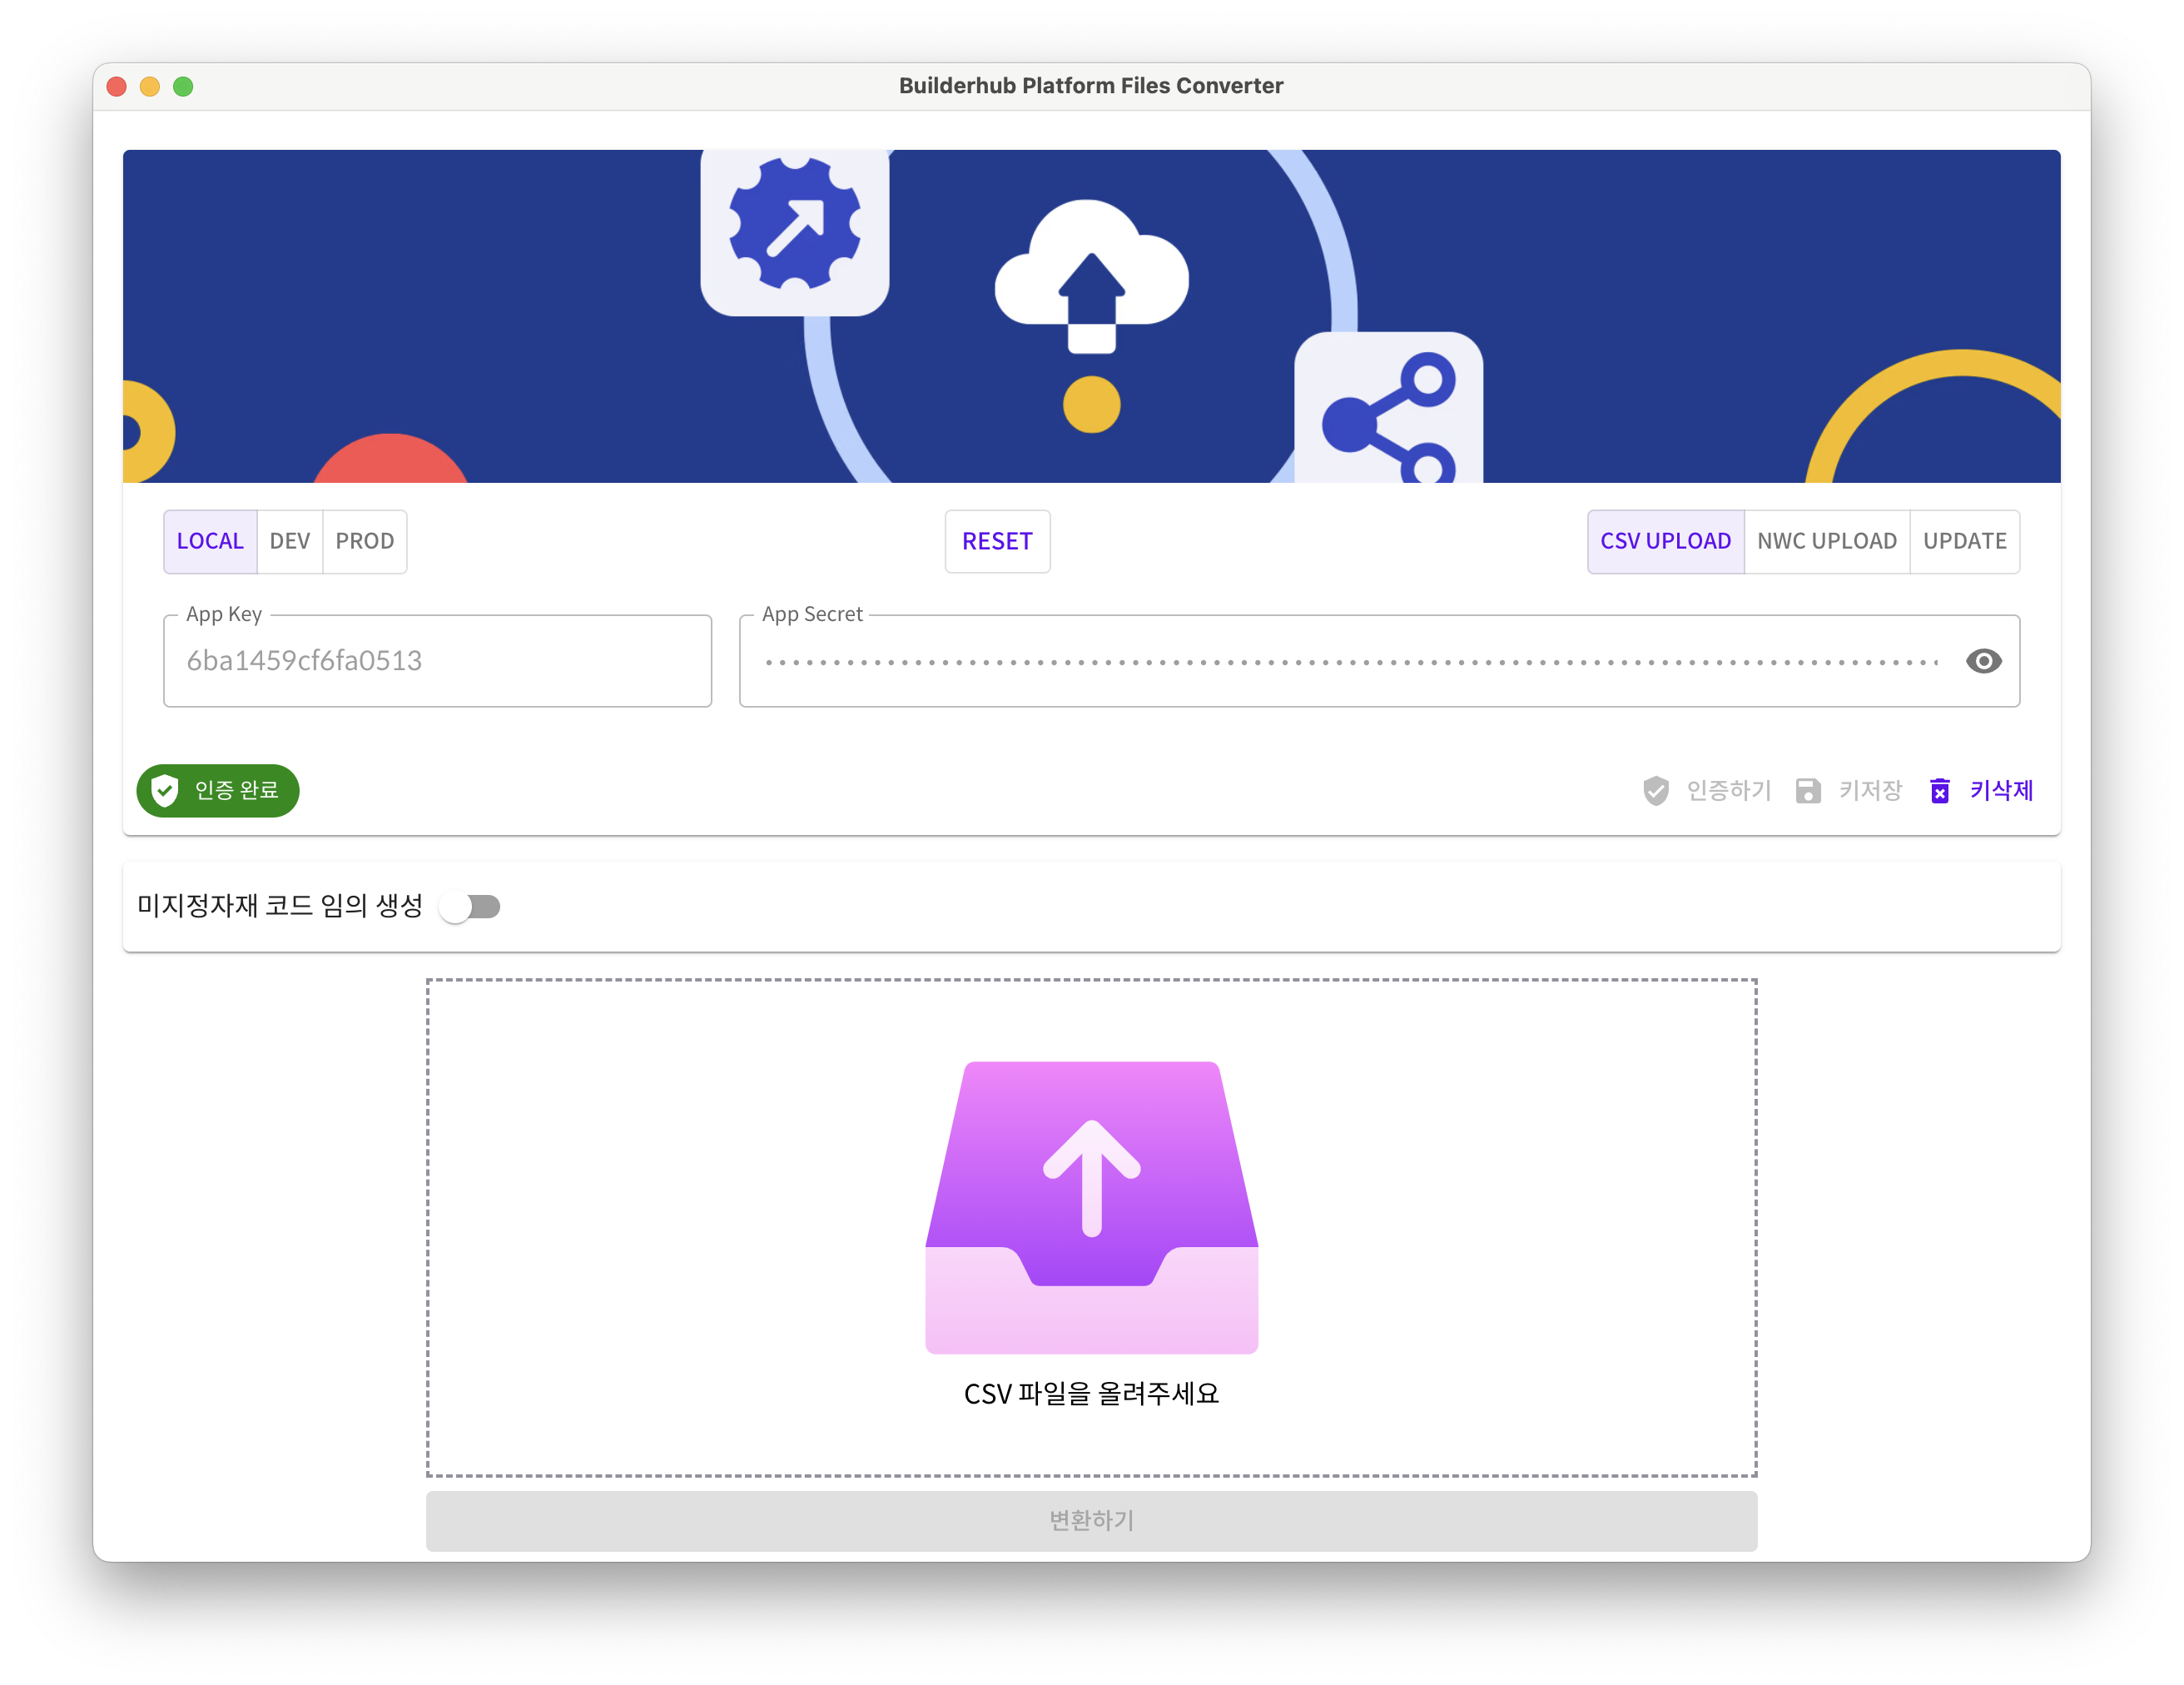
\includegraphics[width=0.25\textwidth]{images/builderhub-converter-auth.png}
					            \caption*{Authorized}
				            }\qquad
				            \parbox{0.45\textwidth}{
					            \centering
					            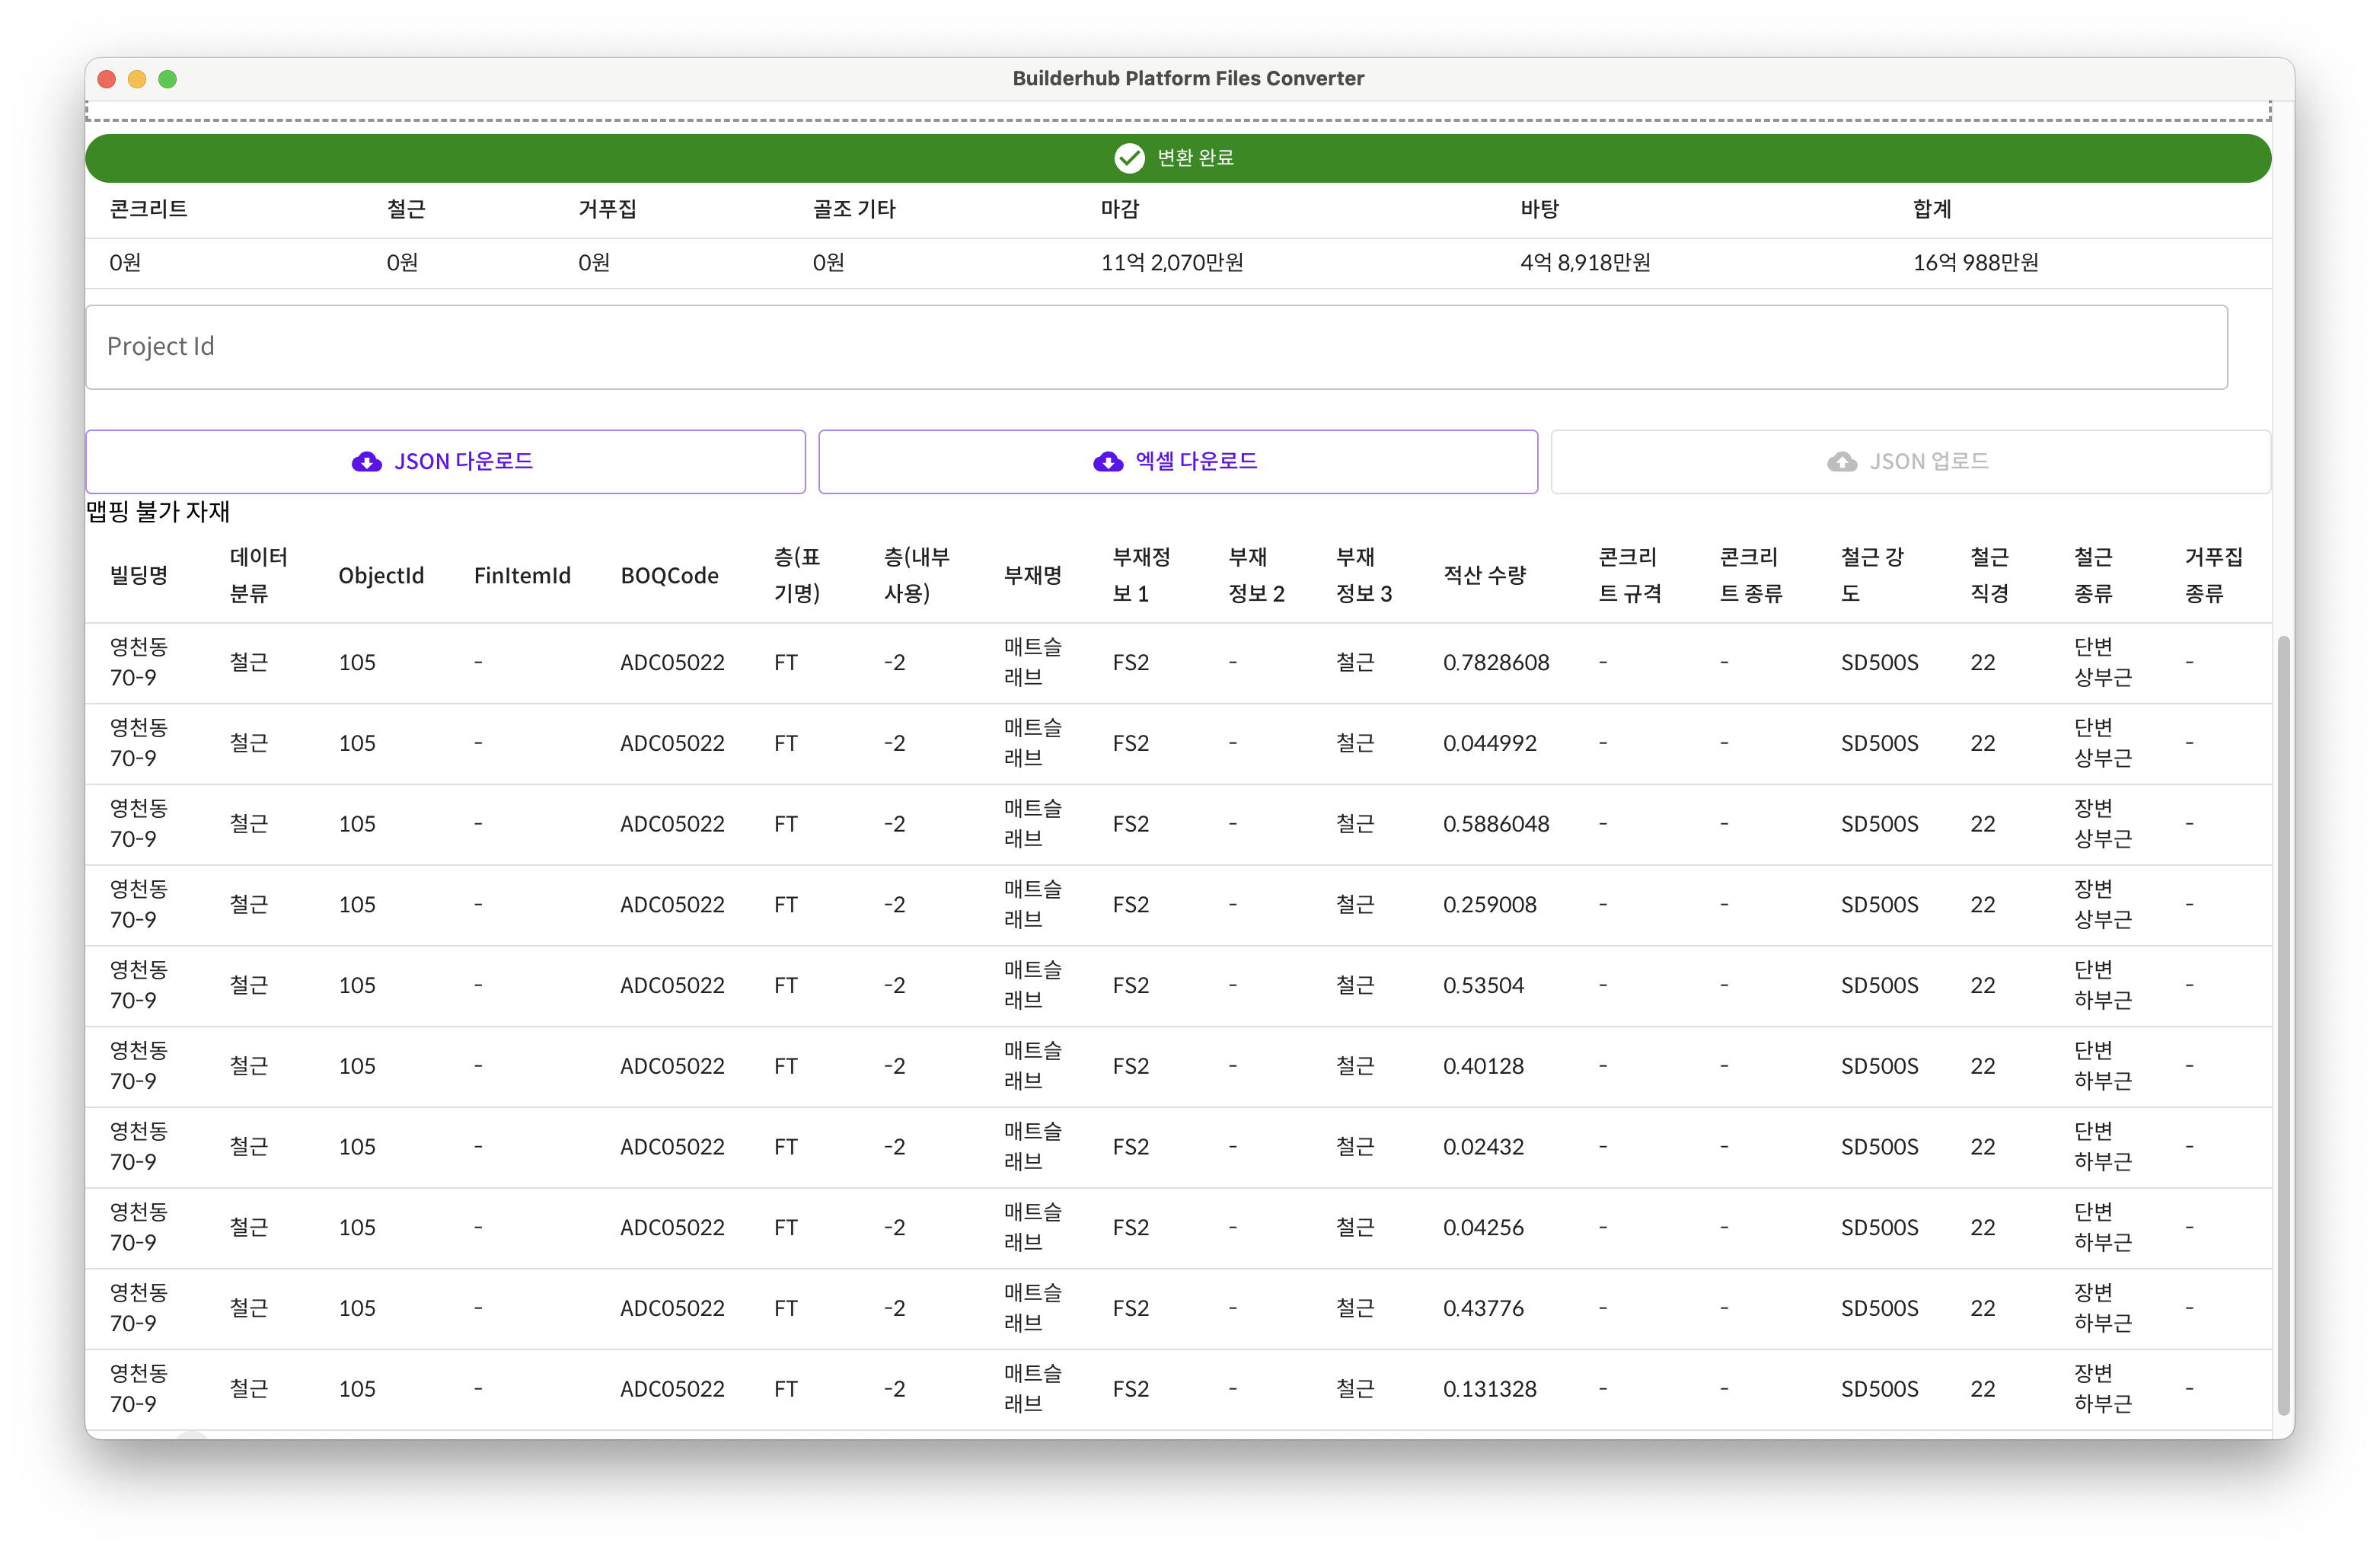
\includegraphics[width=0.28\textwidth]{images/builderhub-converter-converted.png}
					            \caption*{Converted: Mapping}
				            }
			            \end{fullwidth}
		            \end{figure}
		      \item \textbf{인프라 구성}
		            \begin{itemize}
			            \item 1차 코드형 인프라(IaC: AWS Copilot, AWS CDK 2022.06 - 2022.10): AWS CloudFormation, Amplify, Cognito, ALB, RDS, Lambda, API Gateway, S3, CloudFront
			            \item 2차 코드형 인프라(IaC: Terraform 2022.11 - 2023.12): AWS ECS, RDS, Lambda, API Gateway, S3, CloudFront, SES 등
			            \item 3차 쿠버네티스 인프라(IaC: Terraform, Helm Chart 2023.12 - now): EKS, ELB, PostgreSQL, Prometheus, Grafana, ArgoCD, Github Action, Nginx, Supertokens 등
		            \end{itemize}
		            \begin{figure}[!ht]
			            \begin{fullwidth}
				            \parbox{0.8\textwidth}{
					            \centering
					            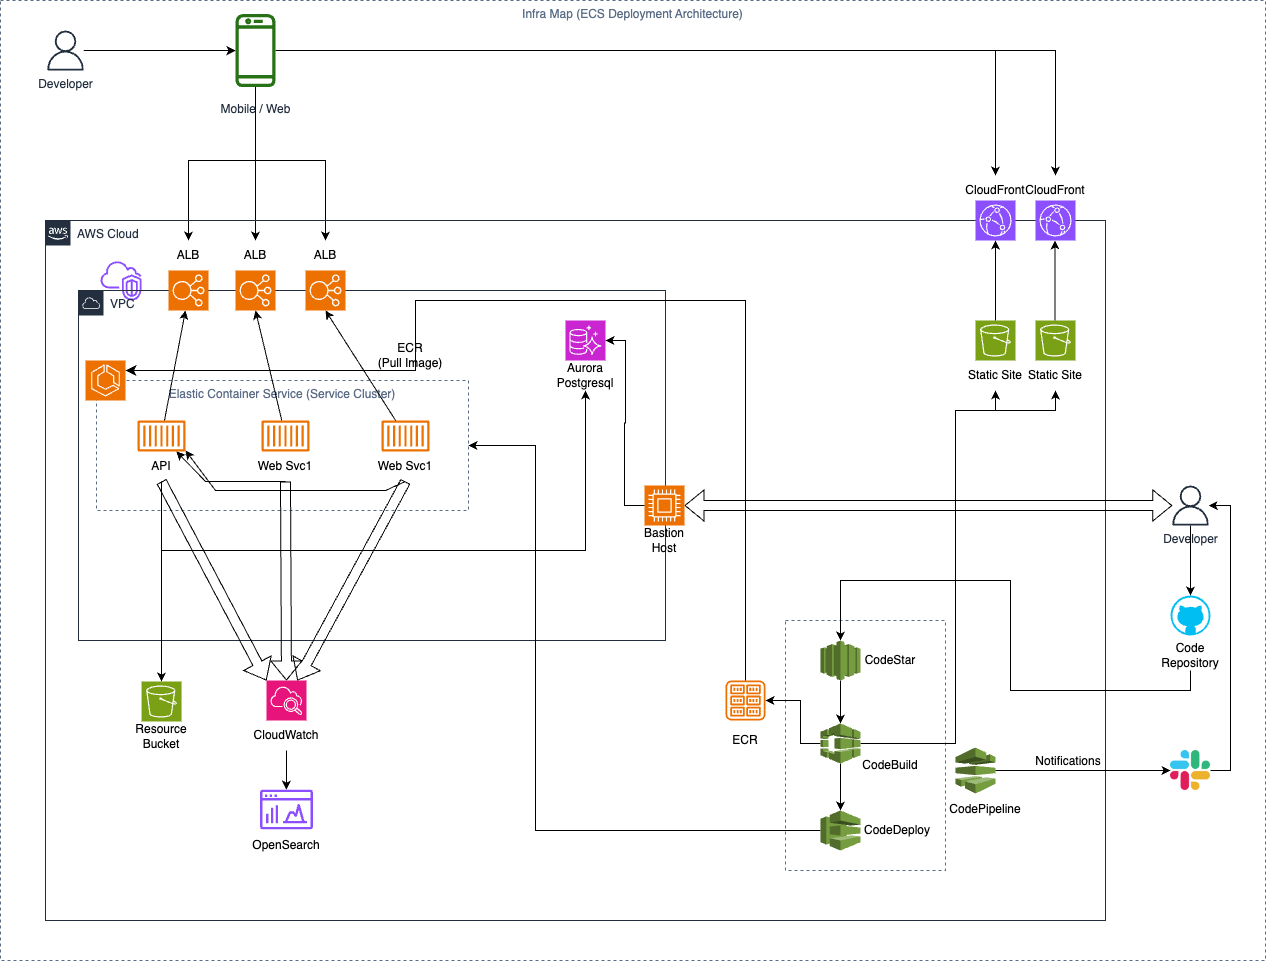
\includegraphics[width=0.40\textwidth]{images/ECS Architecture (bg_white).png}
					            \caption*{ECS Infra}
				            }\qquad
				            \parbox{0.6\textwidth}{
					            \centering
					            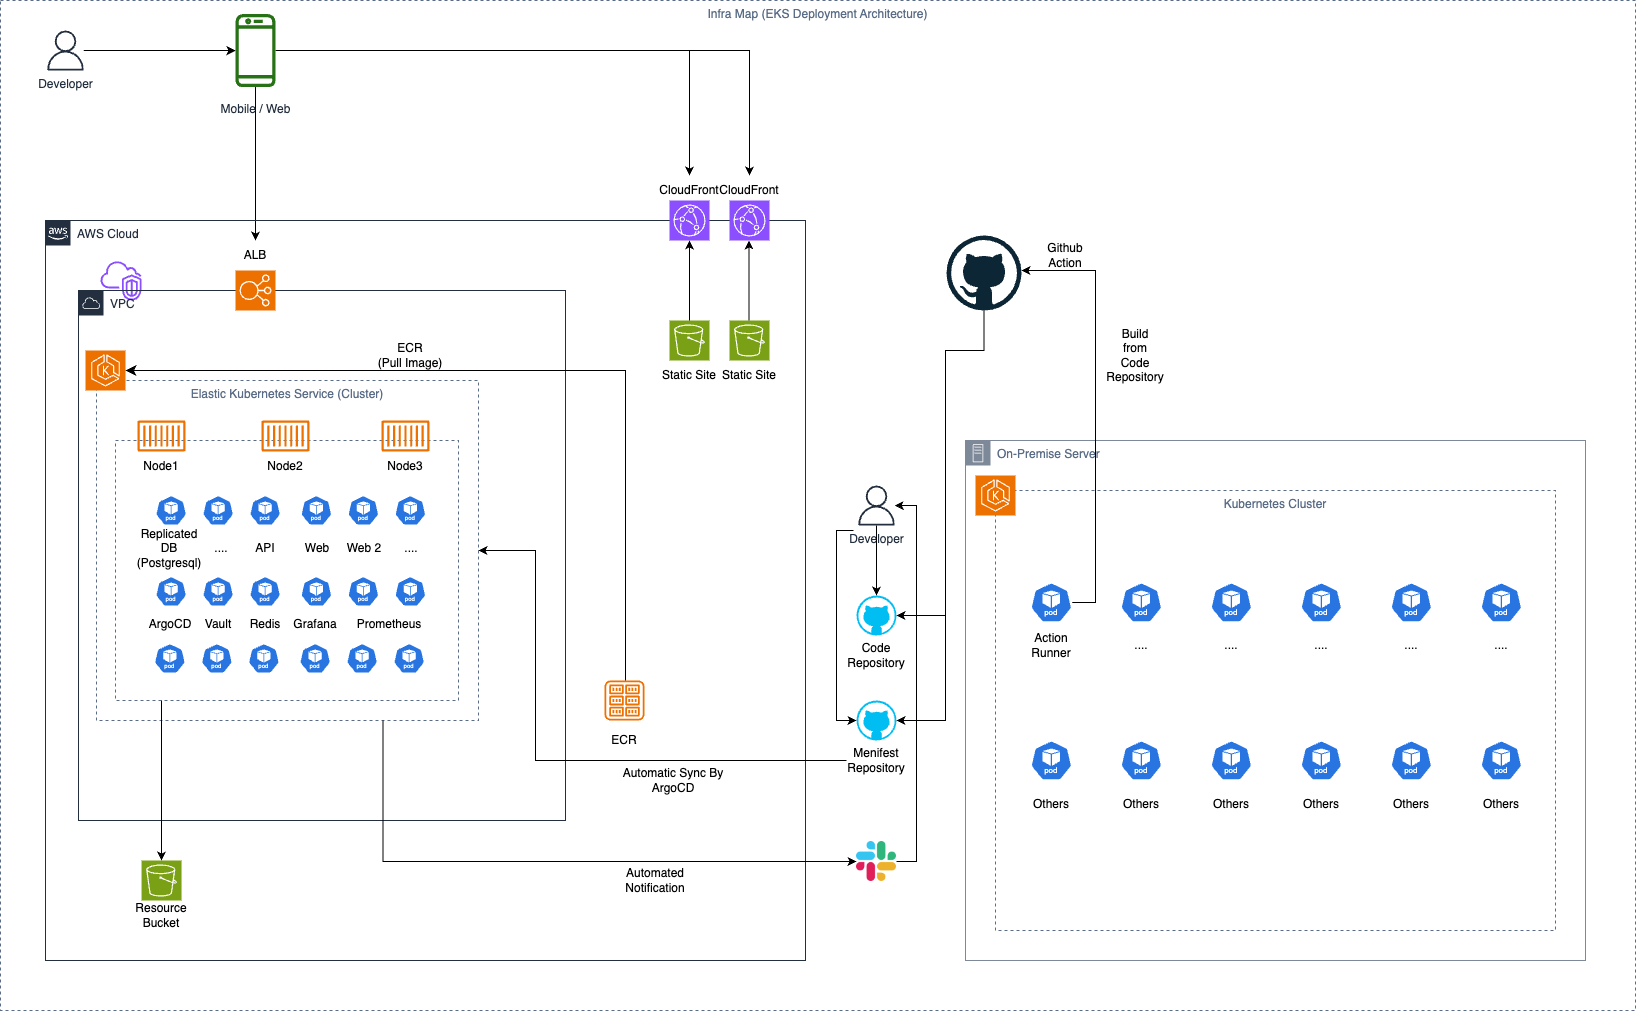
\includegraphics[width=0.5\textwidth]{images/EKS Architecture (bg_white).png}
					            \caption*{EKS Infra}
				            }
			            \end{fullwidth}
		            \end{figure}
		      \item \textbf{백엔드 개발 스택}: TypeScript, NodeJS, Apollo Server, Code first GraphQL Schema, GraphQL Codegen, Nexus Framework, PalJS, OAS REST API 등
		      \item \textbf{프론트엔드 개발 스택}: TypeScript, NextJS, ReactJS, Redux toolkit, XState, Threejs, Autodesk Forge SDK
	      \end{itemize}
\end{itemize}

\cvevent{\printinfo{\faPlusSquare}{\href{https://check.builderhub.io/signin}{스마트체커} 개발(B2B)}}{(주)창소프트아이앤아이 개발리딩}{2023.09 -- now}{Seoul, Korea}

\label{smartchecker}

\begin{itemize}[label=\emoji{satellite}]
	\item 소개: 최근 몇몇 시공사들의 철근을 누락하는 사고를 미연에 예방하기 위해 철근 모니터링 시스템을 도입, 시공사 대상 B2B 프로젝트로 개발리딩
	\item 1차 목표: 자사 솔루션 Builderhub-Q를 사용하고 있는 시공사를 대상으로 적산 물량과 실제 철근 샵도면을 자동 인식하여 물량을 계산하여 비교, 예상 물량과 다를 경우 확인할 수 있도록 서비스 개발. 그리고 도면 체크 상습적으로 철근이 누락되는 구간을 미리 분석하여 도면 승인 이전에 확인할 수 있도록 개발
	\item 참여 개발 내용: 신규 개발 인력 채용, OJT 기간을 거쳐, 전체 프로젝트 개발 리딩
	\item 개발 기간: 3개월
	\item 개발 인원: 4명
	      \begin{figure}[!ht]
		      \begin{fullwidth}
			      \parbox{0.35\textwidth}{
				      \centering
				      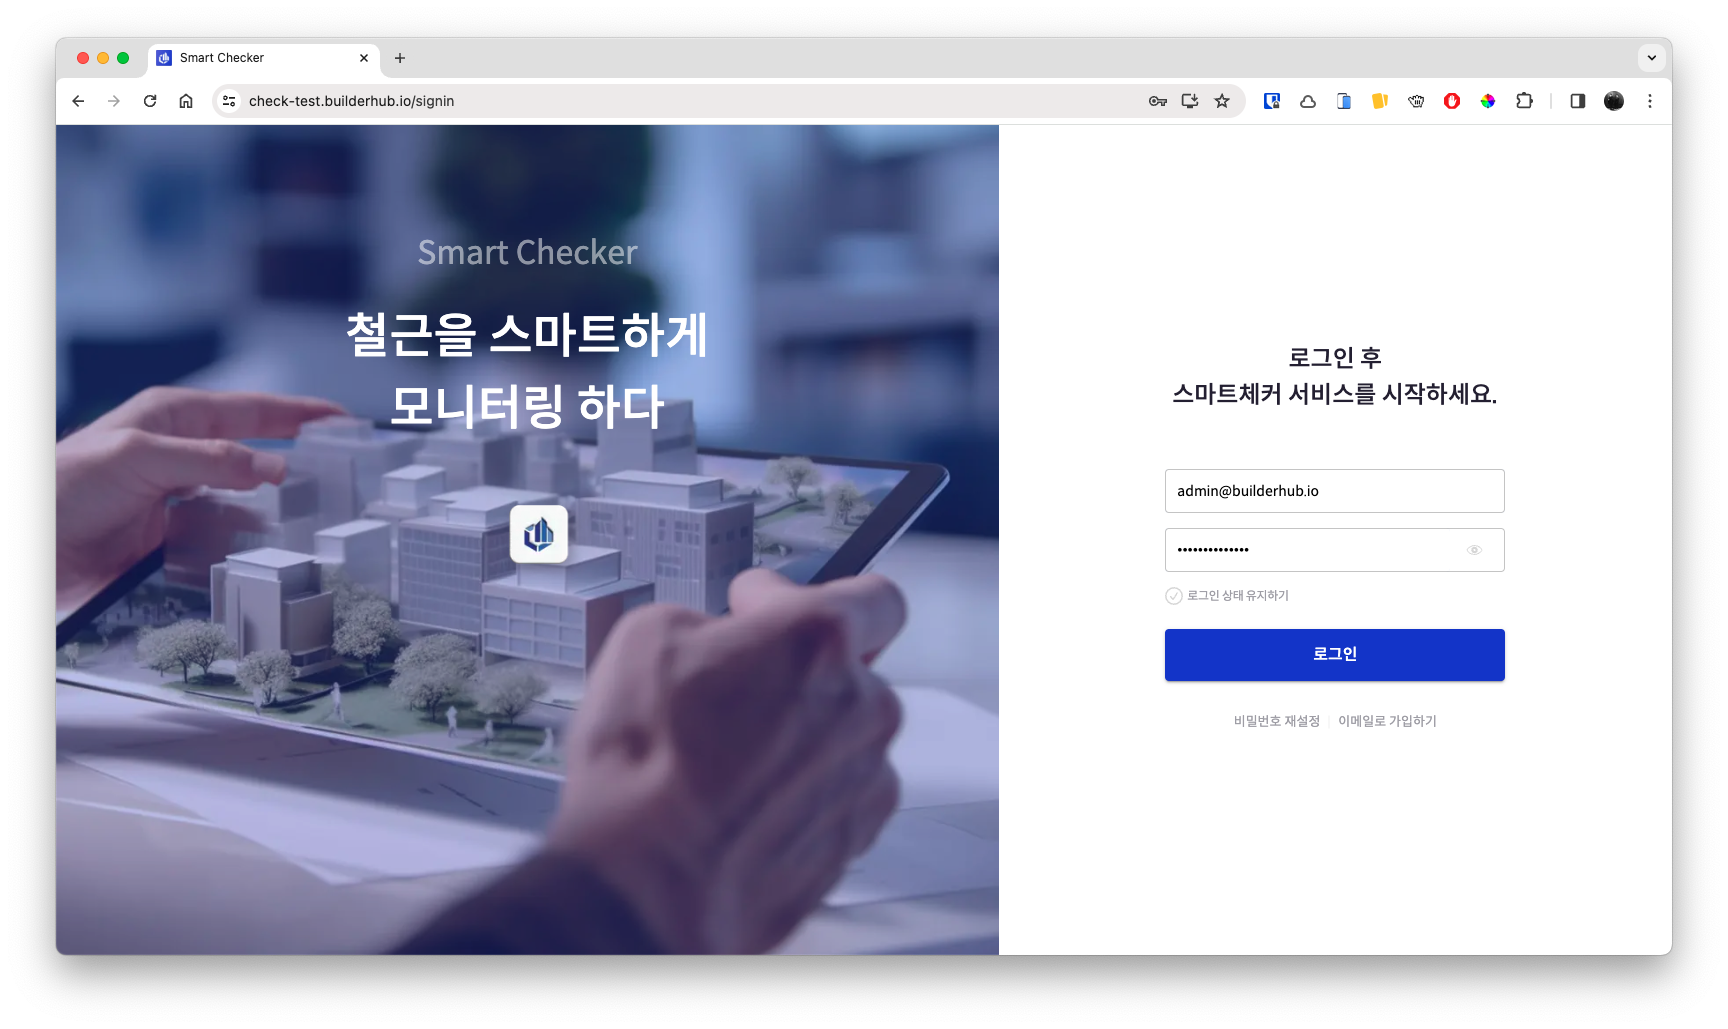
\includegraphics[width=0.35\textwidth]{images/smart-checker-auth.png}
				      \caption*{Authentication}
			      }\qquad
			      \parbox{0.35\textwidth}{
				      \centering
				      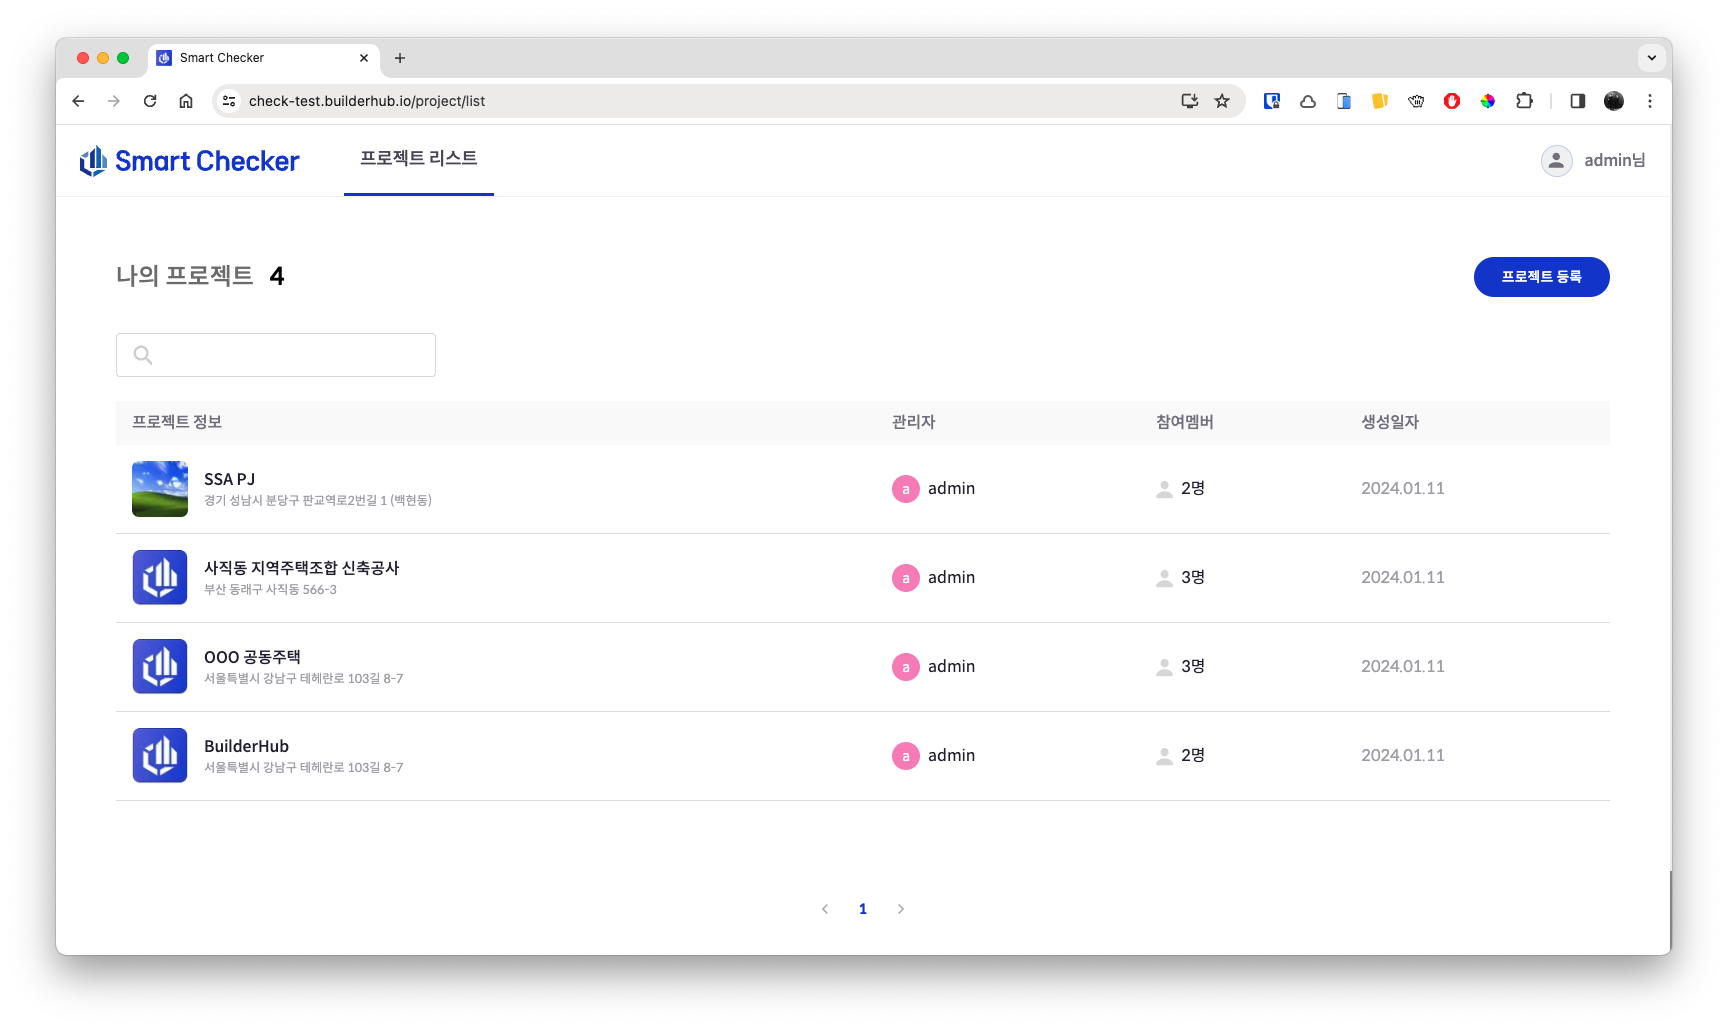
\includegraphics[width=0.35\textwidth]{images/smart-checker-project-list.png}
				      \caption*{Project list}
			      }\qquad
			      \parbox{0.35\textwidth}{
				      \centering
				      \includegraphics[width=0.35\textwidth]{images/smart-checker-project-info.png}
				      \caption*{Project information}
			      }\qquad
			      \parbox{0.35\textwidth}{
				      \centering
				      \includegraphics[width=0.35\textwidth]{images/smart-checker-csv-upload.png}
				      \caption*{CSV upload(BH-Q)}
			      }
			      \parbox{0.35\textwidth}{
				      \centering
				      \includegraphics[width=0.35\textwidth]{images/smart-checker-csv-upload-pivot.png}
				      \caption*{물량 Chart, 피벗테이블}
			      }\qquad
			      \parbox{0.35\textwidth}{
				      \centering
				      \includegraphics[width=0.35\textwidth]{images/smart-checker-dashboard.png}
				      \caption*{Dashboard}
			      }\qquad
			      \parbox{0.35\textwidth}{
				      \centering
				      \includegraphics[width=0.35\textwidth]{images/smart-checker-approval-status.png}
				      \caption*{시공사 승인현황}
			      }\qquad
			      \parbox{0.35\textwidth}{
				      \centering
				      \includegraphics[width=0.35\textwidth]{images/smart-checker-file-browser.png}
				      \caption*{클라우드 파일 관리}
			      }
		      \end{fullwidth}
	      \end{figure}

	\item 개발한 서비스
	      \begin{itemize}[label=\emoji{pushpin}]
		      \item \textbf{스마트체커 서비스}: 자사 솔루션 제품 데이터(Builderhub Q, 2DShopPro)를 활용한 철근 물량 검토 서비스
		      \item \textbf{파일클라우드}: 웹하드 대체를 위한 파일클라우드 개발
		      \item \textbf{도면 컨버터 개발}: 철근 샵도면을 읽어 물량 정보 및 메타데이터를 추출 및 도면 뷰어를 위한 데이터 컨버팅
		      \item \textbf{이슈 트래킹}: 도면 또는 자체 이슈들을 관리하기 위한 이슈관리 서비스 개발 (개발 중)
		      \item \textbf{인프라 구성}:
		            \begin{itemize}
			            \item 쿠버네티스 인프라 구성: EKS, ELB, Prometheus, Grafana, ArgoCD, Github Action, Nginx, Supertokens 등
			            \item Turbo Repo 구성: 모노 리포지토리에서 모든 앱과 패키지들을 통합하여 관리 및 배포
		            \end{itemize}
		      \item \textbf{백엔드 \& 프론트 개발 스택}: TypeScript, NodeJS, Apollo Server, Code first GraphQL Schema, GraphQL Codegen, Nexus Framework, PalJS, OAS REST API, NextJS
	      \end{itemize}

	      \begin{figure}[!ht]
		      \begin{fullwidth}
			      \parbox{0.35\textwidth}{
				      \centering
				      \includegraphics[width=0.35\textwidth]{images/smart-checker-admin-project-list.png}
				      \caption*{어드민: Project List}
			      }\qquad
			      \parbox{0.35\textwidth}{
				      \centering
				      \includegraphics[width=0.35\textwidth]{images/smart-checker-admin-license-list.png}
				      \caption*{어드민: 발급 라이센스}
			      }\qquad
			      \parbox{0.35\textwidth}{
				      \centering
				      \includegraphics[width=0.35\textwidth]{images/smart-checker-admin-license-generation.png}
				      \caption*{어드민: 라이센스 발급}
			      }\qquad
			      \parbox{0.35\textwidth}{
				      \centering
				      \includegraphics[width=0.35\textwidth]{images/smart-checker-admin-org-list.png}
				      \caption*{어드민: 업체 리스트}
			      }
			      \parbox{0.35\textwidth}{
				      \centering
				      \includegraphics[width=0.35\textwidth]{images/smart-checker-sd-upload-chart.png}
				      \caption*{샵도면 업로드 및 골구도차트}
			      }\qquad
			      \parbox{0.35\textwidth}{
				      \centering
				      \includegraphics[width=0.35\textwidth]{images/smart-checker-sd-listing.png}
				      \caption*{샵도면 리스트 및 변환}
			      }\qquad
			      \parbox{0.35\textwidth}{
				      \centering
				      \includegraphics[width=0.35\textwidth]{images/smart-checker-approval.png}
				      \caption*{샵업체 승인현황}
			      }\qquad
			      \parbox{0.35\textwidth}{
				      \centering
				      \includegraphics[width=0.35\textwidth]{images/smart-checker-my-page.png}
				      \caption*{회원 마이페이지}
			      }
		      \end{fullwidth}
	      \end{figure}
\end{itemize}

\cvevent{\printinfo{\faPlusSquare}{건축 감리 B2B 프로젝트 개발: \href{https://asec.builderhub.io/dashboard/detail/initial/supervision}{DEMO}}}{(주)창소프트아이앤아이}{2023.10 -- 2023.11}{Seoul, Korea}

\label{asec}

\begin{itemize}[label=\emoji{satellite}]
	\item 소개: Artifical Structural Engineer \& Construction, ASEC 이란 이름으로 철근 누락 사고의 근본적 원인인 BIM 모델과 매핑된 조립 철근의 ID를 현장에서 바로 사용할 수 있도록 데모 형태로 개발. 건축 구조 엔지니어의 구조 도면과 연동 및 Midas-GEN과 연동
	\item 1차 목표: 자사 솔루션 Builderhub-Q 제품으로 추출된 데이터로 자동 공정표를 생성하여 시공 구역을 산정. 공장가공 철근 ID 구성 및 사진 업로드 기능 구현 
	\item 개발 기간: 3주
	\item 개발 인원: 2명
	\item 개발한 서비스
	      \begin{itemize}[label=\emoji{pushpin}]
		      \item \textbf{건축 공정표}
					\item \textbf{공정 체크리스트}
					\item \textbf{모델 연동}
					\item \textbf{공장 가공 철근 부재별 체크하여 S3 사진 업로드}
					\item \textbf{철근 조립 이후 현장 S3 사진 업로드}
		      \item URL에 해당 데이터 저장
					\item URL Shortener
					\item 공장 가공 철근 QR Code 연동
					\item micro NFC 태그
	      \end{itemize}
\end{itemize}
\begin{figure}[!ht]
	\begin{fullwidth}
		\parbox{0.35\textwidth}{
			\centering
			\includegraphics[width=0.35\textwidth]{images/builderhub-supervision-landing-1.png}
			\caption*{Landing page}
		}\qquad
		\parbox{0.35\textwidth}{
			\centering
			\includegraphics[width=0.35\textwidth]{images/builderhub-supervision-project-list.png}
			\caption*{Project list}
		}\qquad
		\parbox{0.35\textwidth}{
			\centering
			\includegraphics[width=0.35\textwidth]{images/builderhub-supervision-main-1.png}
			\caption*{Supervision}
		}\qquad
		\parbox{0.35\textwidth}{
			\centering
			\includegraphics[width=0.35\textwidth]{images/builderhub-supervision-checklist.png}
			\caption*{Check list}
		}
		\parbox{0.35\textwidth}{
			\centering
			\includegraphics[width=0.35\textwidth]{images/builderhub-supervision-check-member.png}
			\caption*{Member check}
		}\qquad
		\parbox{0.35\textwidth}{
			\centering
			\includegraphics[width=0.35\textwidth]{images/builderhub-supervision-asec.png}
			\caption*{ASEC Check main}
		}\qquad
		\parbox{0.35\textwidth}{
			\centering
			\includegraphics[width=0.35\textwidth]{images/builderhub-supervision-asec-model-check.png}
			\caption*{ASEC Model check}
		}\qquad
		\parbox{0.35\textwidth}{
			\centering
			\includegraphics[width=0.35\textwidth]{images/builderhub-supervision-archi-gantt.png}
			\caption*{Architecture milestones}
		}
	\end{fullwidth}
\end{figure}


\cvevent{\printinfo{\faPlusSquare}{AD.Fi 플랫폼 개발}}{(주)단비코리아 개발리딩}{2020.01 -- 2022.06}{Seoul, Korea}

\begin{itemize}
	\item AD.Fi: 인터넷 WiFi 공유기 광고 시스템(매장 광고 송출, 광고 관리, 매장, 브랜드, 영업사원, 대리점, 총판 관리) 개발
	      \begin{itemize}[label=$\star$]
		      \item 개발 기간: 6개월
		      \item 유지관리 기간: 18개월
		      \item 개발 인원: 5명
		      \item 개발한 서비스
		            \begin{itemize}
			            \item 공유기 광고 송출 페이지: Captive Portal 광고 노출 및 인터넷 연결 허용
			                  \begin{figure}[!ht]
				                  \begin{fullwidth}
					                  \parbox{0.8\textwidth}{
						                  \centering
						                  \includegraphics[width=0.8\textwidth]{images/ad-fi-platform.png}
						                  \caption*{Fi 솔루션 개발}
					                  }\qquad
					                  \parbox{0.68\textwidth}{
						                  \centering
						                  \includegraphics[width=0.68\textwidth]{images/ad-fi.png}
						                  \caption*{공유기 광고 송출}
					                  }
				                  \end{fullwidth}
			                  \end{figure}
			            \item 광고 집계 및 광고 관리 백오피스: 매장주, 영업사원, 대리점, 총판, 브랜드, 브랜드그룹 어드민
			                  \begin{figure}[!ht]
				                  \begin{fullwidth}
					                  \parbox{0.35\textwidth}{
						                  \centering
						                  \includegraphics[width=0.35\textwidth]{images/ad-fi-admin-ad-dashboard.png}
						                  \caption*{광고 송출 현황}
					                  }\qquad
					                  \parbox{0.35\textwidth}{
						                  \centering
						                  \includegraphics[width=0.35\textwidth]{images/ad-fi-admin-ad-manage.png}
						                  \caption*{광고 관리}
					                  }\qquad
					                  \parbox{0.35\textwidth}{
						                  \centering
						                  \includegraphics[width=0.35\textwidth]{images/ad-fi-admin-device-manage.png}
						                  \caption*{공유기 기기 관리}
					                  }\qquad
					                  \parbox{0.35\textwidth}{
						                  \centering
						                  \includegraphics[width=0.35\textwidth]{images/ad-fi-admin-ad-dashboard.png}
						                  \caption*{광고 송출 현황}
					                  }
					                  \parbox{0.35\textwidth}{
						                  \centering
						                  \includegraphics[width=0.35\textwidth]{images/ad-fi-admin-dashboard.png}
						                  \caption*{대시보드: 통계}
					                  }\qquad
					                  \parbox{0.35\textwidth}{
						                  \centering
						                  \includegraphics[width=0.35\textwidth]{images/ad-fi-admin-brand-stat.png}
						                  \caption*{브랜드 어드민: 통계}
					                  }\qquad
					                  \parbox{0.35\textwidth}{
						                  \centering
						                  \includegraphics[width=0.35\textwidth]{images/ad-fi-admin-brand.png}
						                  \caption*{브랜드 관리}
					                  }\qquad
					                  \parbox{0.35\textwidth}{
						                  \centering
						                  \includegraphics[width=0.35\textwidth]{images/ad-fi-admin-agency.png}
						                  \caption*{대리점 관리}
					                  }
				                  \end{fullwidth}
			                  \end{figure}
			            \item 타겟광고 트래킹 시스템 개발
		            \end{itemize}
		      \item 인프라 구성:
		            \begin{figure}[!ht]
			            \begin{fullwidth}
				            \parbox{1.6\textwidth}{
					            \centering
					            \includegraphics[width=1\textwidth]{images/architecture-fi.png}
					            \caption*{AWS 인프라 구성}
				            }
			            \end{fullwidth}
		            \end{figure}
		            \begin{itemize}
			            \item AWS EC2, CodePipeline, AutoScalingGroup, S3, Lambda
			            \item Linux system daemon(systemd) and timer
			            \item Docker swarm stack: Microservice containers
		            \end{itemize}
		            \begin{figure}[!ht]
			            \begin{fullwidth}
				            \parbox{1.6\textwidth}{
					            \centering
					            \includegraphics[width=1.6\textwidth]{images/deployment-pipeline.png}
					            \caption*{AWS 배포 파이프라인}
				            }
			            \end{fullwidth}
		            \end{figure}
		      \item 백엔드 개발 스택
		            \begin{itemize}
			            \item Type-safe pipeline: TypeScript, NodeJS, Express, Apollo Server, Prisma ORM, Nexus GraphQL, Open API Spec. v3
			            \item Code-first GraphQL schema: Nexus-GraphQL
			            \item Asynchronosus API: Mosquitto, MQTTjs, Async API
		            \end{itemize}
		      \item 프론트 개발 스택
		            \begin{itemize}
			            \item TypeScript, ReactJS, Context API, Material UI, Styled Component, JSS
			            \item GraphQL-codegen(React, Apollo-client)
		            \end{itemize}
	      \end{itemize}
	      \begin{figure}[!ht]
		      \begin{fullwidth}
			      \parbox{1.6\textwidth}{
				      \centering
				      \includegraphics[width=0.3\textwidth]{images/ad-fi-reward.png}
				      \caption*{AD.Fi Captive portal}
			      }
		      \end{fullwidth}
	      \end{figure}
\end{itemize}

\cvevent{\printinfo{\faPlusSquare}{Log.Fi(매장 코로나 19 방명록) 개발}}{(주)단비코리아}{2020.06 -- 2020.06}{Seoul, Korea}

\begin{itemize}
	\item 개발 기간: 2주
	\item 개발 인력: 1인
	\item 개발한 서비스
	      \begin{itemize}
		      \item 체크인 페이지: Captive Portal 브라우저에서 방문자 기록
		      \item 어드민 개발: 사용자 리스트
		      \item 이후 공유기 설정 및 등록 페이지로 활용, 공유기 가등록 및 판매
	      \end{itemize}
\end{itemize}

\cvevent{\printinfo{\faPlusSquare}{Lucky.Fi(매장 경품추첨 앱) 개발}}{(주)단비코리아 개발리딩}{2021.06 -- 2021.06}{Seoul, Korea}

\begin{itemize}
	\item Lucky.Fi(매장 경품추첨 앱) 개발
	      \begin{itemize}[label=$\star$]
		      \item 개발 기간: 4주
		      \item 개발 인력: 5인
		      \item 개발한 서비스
		            \begin{itemize}
			            \item 룰렛 게임: Captive Portal 브라우저에서 룰렛게임, 당첨자 회원가입
			            \item 상품 연동: 쿠프마케팅 기프티콘, 밀크코인
			            \item 코인 적립: SRT 코인 적립
			            \item 브라우저 핑거프린트: 사용자 특정 및 매장 방문 확인
		            \end{itemize}
	      \end{itemize}
\end{itemize}

\cvevent{\printinfo{\faPlusSquare}{공공 WiFi 플랫폼 개발}}{(주)단비코리아}{2021.06 -- 2021.06}{Seoul, Korea}

\begin{itemize}
	\item 강릉시 공공 WiFi 개발, 코엑스 전시장 AD.Fi 서비스
	      \begin{itemize}[label=$\star$]
		      \item 개발 기간: 4주
		      \item 개발 인력: 2인
		      \item 개발한 서비스
		            \begin{itemize}
			            \item 공공 와이파이 연동: Xirrus, Meraki, Lucus 공유기 연동, Grant API 개발
			            \item RADIUS 인증 연동: 자사 RADIUS 서버 연동, 사용자 정보 트래킹
		            \end{itemize}
		            \begin{figure}[!ht]
			            \begin{fullwidth}
				            \parbox{0.35\textwidth}{
					            \centering
					            \includegraphics[width=0.35\textwidth]{images/public-ad-fi-upper-banner.png}
					            \caption*{상단배너 관리}
				            }\qquad
				            \parbox{0.35\textwidth}{
					            \centering
					            \includegraphics[width=0.35\textwidth]{images/public-ad-fi-lower-banner.png}
					            \caption*{하단배너 관리}
				            }\qquad
				            \parbox{0.35\textwidth}{
					            \centering
					            \includegraphics[width=0.35\textwidth]{images/public-ad-fi-device-manage.png}
					            \caption*{기기관리}
				            }\qquad
				            \parbox{0.35\textwidth}{
					            \centering
					            \includegraphics[width=0.35\textwidth]{images/public-ad-fi-preview.png}
					            \caption*{미리보기}
				            }
			            \end{fullwidth}
		            \end{figure}
		      \item 인프라 구성:
		            \begin{itemize}
			            \item Bare Metal 서버 구축
			            \item Docker swarm stack: Traefik, MongoDB Cluster
		            \end{itemize}
		      \item 풀 개발 스택
		            \begin{itemize}
			            \item TypeScript, NodeJS, NextJS, Prisma ORM(MongoDB), Redux Toolkit Query
			            \item GraphQL-codegen(Apollo-client)
		            \end{itemize}
	      \end{itemize}
	      \begin{figure}[!ht]
		      \begin{fullwidth}
			      \parbox{1.6\textwidth}{
				      \centering
				      \includegraphics[width=0.3\textwidth]{images/public-ad-fi-gn-captiveportal.png}
				      \caption*{공공 WiFi Captive portal}
			      }
		      \end{fullwidth}
	      \end{figure}
\end{itemize}

\cvevent{\printinfo{\faPlusSquare}{Cash.Fi(매장 모객 서비스) 백엔드 개발}}{(주)단비코리아 개발리딩}{2021.06 -- 2021.06}{Seoul, Korea}

\begin{figure}[!ht]
	\begin{fullwidth}
		\parbox{1.6\textwidth}{
			\centering
			\includegraphics[width=0.5\textwidth]{images/cash-fi.png}
			\caption*{Cash Fi}
		}
	\end{fullwidth}
\end{figure}
\begin{itemize}
	\item Cash.Fi(매장 모객 서비스) 백엔드 개발
	      \begin{itemize}[label=$\star$]
		      \item 총 개발 기간: 19개월 (외주 관리)
		      \item 해당 개발 기간: 6주
		      \item 개발 인력: 1인
		      \item 개발한 서비스
		            \begin{itemize}
			            \item WiFi indoor position: WiFi 공유기와 Captive portal 연동, 매장 내부 위치 트래킹
			            \item WiFi 공유기 매장 fingerprint 수집: 공유기 AP를 이용 매장 특정 Fingerprint 개발(7종의 ML 알고리즘)
			            \item 외주 개발 백엔드 마이그레이션: DB 마이그레이션, AD-Fi 매장 연동
		            \end{itemize}
		      \item 인프라 구성:
		            \begin{itemize}
			            \item AWS EC2, RDS, S3, Lambda, CloudFront
			            \item Docker swarm stack: Traefik
		            \end{itemize}
		      \item 백엔드 스택
		            \begin{itemize}
			            \item TypeScript, NodeJS, Express, Apollo Server, Prisma ORM
		            \end{itemize}
	      \end{itemize}
\end{itemize}

\cvevent{\printinfo{\faPlusSquare}{스마트팩토리 IIoT PdM 플랫폼 개발}}{(주)아프로스 개발참여: 100\%}{2018.03 -- 2019}{Seoul, Korea}

\begin{itemize}[label=\emoji{satellite}]
	\item 소개: 스마트팩토리 IIoT PdM 솔루션 개발
	\item 참여 개발 내용: Edge Device(DAQ/Analysis) 애플리케이션 개발, 웹플랫폼 개발
	\item 개발 스택 및 프레임워크: *nix, NodeJS N-API, C++, golang, Python, Redis, MongoDB, GraphQL, ReactJS
	\item 참여 개발 내용
	      \begin{itemize}[label=\emoji{pushpin}]
		      \item 데이터 분석: Diagnosis(HMB-SD 기법 적용, Deep analyzed features), Prognosis(유사성기반 RUL 추정기법)
		      \item Anomaly detection, Disgnosis, Prognosis, Transient event 분류 데이터 누적
		      \item MQTT 브로커, Kafka 분산 메시지 큐, DB구축, GraphQL API 구축
		      \item 디바이스 관리 클라이언트, 플랫폼 클라이언트 개발 (ReactJS)
	      \end{itemize}
	\item 개발 스택 및 프레임워크: JavaScript(ES6), Babel, NodeJS, C++, golang, GraphQL, ReactJS, ElectronJS, Python
	\item 현장 테스트베드 가동: SK하이닉스, SK텔레콤, KETI, 남강정밀등. 80여개소 디플로이 및 유지관리
\end{itemize}
\begin{figure}[!ht]
	\begin{fullwidth}
		\parbox{0.5\textwidth}{
			\centering
			\includegraphics[width=0.5\textwidth]{images/new_dashboard_02.png}
			\caption*{Anomaly detection}
		}\qquad
		\parbox{0.5\textwidth}{
			\centering
			\includegraphics[width=0.5\textwidth]{images/new_dashboard_03.png}
			\caption*{Fault detection}
		}\qquad
		\parbox{0.5\textwidth}{
			\centering
			\includegraphics[width=0.5\textwidth]{images/new_dashboard_05.png}
			\caption*{데이터 조회}
		}
		\parbox{0.5\textwidth}{
			\centering
			\includegraphics[width=0.5\textwidth]{images/new_dashboard_06.png}
			\caption*{Trending / Anomaly map}
		}\qquad
		\parbox{0.5\textwidth}{
			\centering
			\includegraphics[width=0.5\textwidth]{images/new_dashboard_04.png}
			\caption*{설비 상태 모니터링}
		}\qquad
		\parbox{0.5\textwidth}{
			\centering
			\includegraphics[width=0.5\textwidth]{images/mcdl-01.png}
			\caption*{Data logger tool (ElectronJS)}
		}
	\end{fullwidth}
\end{figure}

\divider


\cvevent{\printinfo{\faPlusSquare}{철도 콘크리트 도상 균열 자동 탐지 과제}}{승화기술정책연구소(주) 개발참여: 100\%}{2017 -- 2017}{Seoul, Korea}

\begin{itemize}
	\item 소개: 철도 콘크리트 도상 균열 자동 탐지 과제
	\item 참여 개발 내용: 연구책임자
	      \begin{itemize}
		      \item 레이저 라인 스캔카메라를 이용한 고해상도 이미지 취득후 균열 탐지 (0.3x0.22mm)
		      \item Phothmetric normalization과 B-COSFIRE Filter(DoG response)를 사용하여 TCL층의 라인구조식별
		      \item Machine learning(support vector machine)을 이용하여 도상 구조물과 균열을 분류
		      \item 분류된 균열 그리고 도상 구조물을 ground truth로 분리하여 CNN(convolutional neural network) 학습.
	      \end{itemize}
	\item 개발 스택 및 프레임워크: MATLAB, Python, Tensor flow(CNN), OpenCV
	\item 현장 테스트베드 가동(Trolley 방식), 선로검측차 탑재
	\item \href{https://www.eunchurn.com/blog/engineering/2017-12-30-concrete-cracks-detection-using-b-cosfire-filter}{링크 참조}
\end{itemize}

\begin{figure}[ht]
	\begin{fullwidth}
		\parbox{0.5\textwidth}{
			\centering
			\includegraphics[width=0.5\textwidth]{images/zoomed_dog.png}
			\caption*{균열과 구조물 분리}
		}\qquad
		\parbox{0.5\textwidth}{
			\centering
			\includegraphics[width=0.5\textwidth]{images/zoomed.png}
			\caption*{균열 ground truth 지정}
		}\qquad
		\parbox{0.5\textwidth}{
			\centering
			\includegraphics[width=0.5\textwidth]{images/crack06.png}
			\caption*{0.2mm 미세균열 검출}
		}
	\end{fullwidth}
\end{figure}

\divider

\cvevent{\printinfo{\faPlusSquare}{KTX 승객 검표지원 시스템 지능형 CCTV \& MTIT 연동}}{승화기술정책연구소(주) 개발참여: 100\%}{2016 -- 2017}{Seoul, Korea}

\begin{itemize}
	\item 소개: 컴퓨터 비젼(OpenCV) 및 이미지 프로세싱을 이용한 승객 착석유무 판단
	\item 참여 개발 내용: 현장 CCTV를 통해 이미지 취득 후 컴퓨터 비젼 프로세싱
	\item 개발 스택 및 프레임워크: C++ 기반 OpenCV, JavaScript(ES5), NodeJS, Express, EJS, Redis, MongoDB
	\item KTX 1편성, ITX-청춘 1편성 현장 적용 완료
\end{itemize}

\begin{figure}[!ht]
	\begin{fullwidth}
		\parbox{0.5\textwidth}{
			\centering
			\includegraphics[width=0.5\textwidth]{images/korail_seat_01_01.png}
			\caption*{무임 승차자 검출}
		}\qquad
		\parbox{0.5\textwidth}{
			\centering
			\includegraphics[width=0.5\textwidth]{images/korail_seat_01_02.png}
			\caption*{MTIT 발권 데이터 요청/응답}
		}\qquad
		\parbox{0.5\textwidth}{
			\centering
			\includegraphics[width=0.5\textwidth]{images/korail_seat_02.jpg}
			\caption*{Raspberry Pi 탑재용 테스트 프로그램}
		}
	\end{fullwidth}
\end{figure}

\divider


\cvevent{\printinfo{\faPlusSquare}{철도 재해우려개소 지능형 CCTV 낙석감지 시스템}}{승화기술정책연구소(주) 개발참여: 95\%}{2016 -- 2017}{Seoul, Korea}

\begin{itemize}
	\item
	      소개: 컴퓨터 비젼(OpenCV) 및 이미지 프로세싱을 이용한 낙석감지 알람
	\item 참여 개발 내용
	      \begin{itemize}
		      \item 현장 CCTV를 통해 이미지 취득 후 컴퓨터 비젼 프로세싱
		      \item 애플리케이션 개발: Raspberry Pi, NodeJS 애플리케이션(OpenCV, nodeJS, Redis, MongoDB 웹서버 및 UI가동)
	      \end{itemize}
	      \begin{figure}[!ht]
		      \begin{fullwidth}
			      \parbox{0.5\textwidth}{
				      \centering
				      \includegraphics[width=0.5\textwidth]{images/korail_aod_01.jpg}
				      \caption*{OpenCV 애플리케이션}
			      }\qquad
			      \parbox{0.5\textwidth}{
				      \centering
				      \includegraphics[width=0.5\textwidth]{images/korail_aod_02.jpg}
				      \caption*{이벤트 발생 기록}
			      }\qquad
			      \parbox{0.5\textwidth}{
				      \centering
				      \includegraphics[width=0.5\textwidth]{images/korail_aod_03_01.png}
				      \caption*{이벤트 뷰 > SMS 메시지 전송}
			      }
		      \end{fullwidth}
	      \end{figure}

	\item 개발 스택 및 프레임워크
	      \begin{itemize}
		      \item C++ 기반 OpenCV
		      \item NVidia Jetson TX-1을 이용한 컴퓨터 비전 활용
		      \item JavaScript(ES5), NodeJS, Express, SocketIO 푸시 알림 웹서버 (Redis, MongoDB)
	      \end{itemize}
	\item 현장 테스트베드 가동, 160여개소 적용 준비
\end{itemize}

\divider

\cvevent{\printinfo{\faPlusSquare}{지하철 역사 초기 재난 대응 M2M 대피경로 안내 시스템}}{승화기술정책연구소(주) 개발참여: 80\%}{2015 -- 2017}{Seoul, Korea}

\begin{itemize}
	\item 소개: 가스센서 노드로부터 데이터를 받아 화재 및 재난을 초기 인식하여 승객들에게 대피경로를 안내하는 시스템
	\item 참여 개발 내용:
	      \begin{itemize}
		      \item Libelium Waspmote기반 가스센서 펌웨어 개발
		      \item 가스센서 Calibration : MATLAB을 이용하여 기준값 측정 후 곡선적합
		      \item 게이트웨이 개발: Raspberry Pi \href{https://nodejs.org}{nodeJS} 애플리케이션(serial parsing, Redis, MongoDB, 웹서버 및 클라이언트 개발)

		            \begin{figure}[!ht]
			            \begin{fullwidth}
				            \centering
				            \parbox{0.8\textwidth}{
					            \includegraphics[width=0.8\textwidth]{images/m2m_01.png}
					            \caption*{실시간 센서 모니터링}
				            }\qquad
				            \parbox{0.8\textwidth}{
					            \includegraphics[width=0.8\textwidth]{images/m2m_02.png}
					            \caption*{센서 캘리브레이션, 데이터 조회}
				            }
			            \end{fullwidth}
		            \end{figure}
		      \item 센서노드 API 제작(Plug\&Sense): sleep time 스케쥴링
		      \item 화재 감지 및 화재 발생 위치 분석: 주요요소분석(principal component analysis, 각 센서데이터의 확률밀도함수와 이벤트간 주요요소분석), 확률변수시물레이션(Monte-Carlo 시물레이션)
		      \item Markov-chain 룰을 통해 상태예측 알고리즘 개발
		      \item 대피경로 안내 시스템 개발(역무원용/승객 알림용)
		            \begin{figure}[ht!]
			            \begin{fullwidth}
				            \centering
				            \includegraphics[width=1.2\textwidth]{images/m2m_03.png}
				            \caption*{대피경로 안내 시나리오 설정}
			            \end{fullwidth}
		            \end{figure}
		            \begin{figure}[ht!]
			            \begin{fullwidth}
				            \centering
				            \includegraphics[width=1.2\textwidth]{images/m2m_04.png}
				            \caption*{승객용 재난 발생 위치 알림}
			            \end{fullwidth}
		            \end{figure}
		            \begin{figure}[ht!]
			            \begin{fullwidth}
				            \centering
				            \includegraphics[width=1.2\textwidth]{images/m2m_05.png}
				            \caption*{센서 Matrix Rule set 지정}
			            \end{fullwidth}
		            \end{figure}
	      \end{itemize}
	\item 적용된 기술:
	      \begin{itemize}
		      \item \href{https://en.wikipedia.org/wiki/Machine_to_machine}{M2M}
		      \item \href{https://lora-alliance.org/}{LoRa} 802.11ah SX1274 916MHz
		      \item \href{https://en.wikipedia.org/wiki/Principal_component_analysis}{Principal component analysis}
		      \item \href{https://en.wikipedia.org/wiki/Monte_Carlo_method}{Monte Carlo method}
		      \item \href{https://en.wikipedia.org/wiki/Markov_chain}{Markov chain}
	      \end{itemize}
	\item 개발 스택 및 프레임워크
	      \begin{itemize}
		      \item 적합성 데이터 분석 및 센서 캘리브레이션: Mathworks MATLAB
		      \item 센서 관리 웹어드민: JavaScript(ES5), NodeJS, Express, React, Webpack
		      \item 센서 데이터 송신 펌웨어: C (Libelium SDK)
		      \item 센서 특징 정보 추출: Python
		      \item 대피경로 안내 시스템: Django
	      \end{itemize}
	\item 참여한 현장: 대공원역 / 개포동역
\end{itemize}


\divider

\cvevent{\printinfo{\faPlusSquare}{도로 안개 소산 시스템 프로젝트}}{Korea Maintenance 개발참여: 100\%}{2014 -- 2019}{Seoul, Korea}

\begin{itemize}
	\item 소개: 온풍, 음이온 생성기, 응결핵등을 방사하여 도로상에 안개를 신속히 제거하는 시스템
	\item 참여 개발 내용
	      \begin{itemize}
		      \item CCTV 영상이미지를 이용한 안개시정거리 계산: \href{https://en.wikipedia.org/wiki/Feature_detection_(computer_vision)}{Feature detection}
		      \item 오브젝트 트래킹 문제: \href{https://en.wikipedia.org/wiki/Partial_least_squares_regression}{Partial least square analysis}를 통해 타깃의 위치 판탄 (2stage filtering)
		      \item \href{http://www4.comp.polyu.edu.hk/~cslzhang/CT/CT.htm}{Real-time compressive tracking}: \href{https://en.wikipedia.org/wiki/Filter_bank}{multiscale filterbank}를 통해 \href{https://en.wikipedia.org/wiki/Feature_detection_(computer_vision)}{feature detection} 후 매트릭스방식의 feature를 벡터화
		      \item 오브젝트 트래킹 에러로 success rate, average center location error를 판단하여 시정거리와 매핑.
		      \item \href{https://siddhantahuja.wordpress.com/tag/sum-of-squared-differences/}{Sum of squared difference} \/ \href{https://en.wikipedia.org/wiki/Cross-correlation\#Normalized_cross-correlation}{Normalized cross-correlation} 으로 최종 매핑 스코어 판정
		      \item CCTV 이미지를 통해 안개소산장치를 ON/OFF 제어 : 평균화 방식의 \href{https://en.wikipedia.org/wiki/PID_controller}{PID 제어기}로 설계
	      \end{itemize}
	      \begin{figure}[!ht]
		      \begin{fullwidth}
			      \centering
			      \parbox{1.2\textwidth}{
				      \includegraphics[width=1.2\textwidth]{images/fog_02_01.png}
				      \caption*{Fog cannon controller}
			      }\qquad
			      \parbox{0.3\textwidth}{
				      \includegraphics[width=0.3\textwidth]{images/fog_03.png}
				      \caption*{시정거리 계산 / PID 제어}
			      }
		      \end{fullwidth}
	      \end{figure}
\end{itemize}

\divider

\cvevent{\printinfo{\faPlusSquare}{능동형 제진장치 (\href{https://deicon.com/solutions/tuned-mass-dampers/active-tuned-mass-dampers-active-mass-dampers/#:~:text=Active%20Mass%20Damper%20(AMD)%20is,used%20in%20broadband%20vibration%20abatement.}{Active \& Hybrid Mass Damper, A-HMD})개발 및 웹 모니터링 서비스 개발}}{Korea Maintenance \& APROS 개발참여: 100\%}{2014 -- 2019}{Seoul, Korea}

\begin{itemize}
	\item 소개: 건물의 사용중 진동 저감을 위한 능동형 제진장치 설치 및 모니터링 플랫폼 개발 프로젝트
	\item 참여 개발 내용:
	      \begin{itemize}
		      \item \href{http://www.quanser.com/products/active_mass_damper}{Quansar 소형 AMD 제어}, \href{https://en.wikipedia.org/wiki/Linear-quadratic_regulator}{LQR}/\href{https://en.wikipedia.org/wiki/Linear-quadratic-Gaussian_control}{LQG} 알고리즘 탑재.
		      \item 실제 현장에서 계측데이터 품질 확보를 위한 signal conditioning
		      \item High-resolution DAQ 적용
		      \item Raspberry Pi를 이용한 PLC, DAQ, Anemometer 데이터 송출
		      \item MQTT Broker를 통한 데이터 표출 API 개발
		      \item 모니터링 웹애플리케이션 개발
	      \end{itemize}
	      \begin{figure}[!ht]
		      \begin{fullwidth}
			      \parbox{0.5\textwidth}{
				      \centering
				      \includegraphics[width=0.5\textwidth]{images/TM21 Vibration Controller Monitroing - landing.png}
				      \caption*{Landing page}
			      }\qquad
			      \parbox{0.5\textwidth}{
				      \centering
				      \includegraphics[width=0.5\textwidth]{images/TM21 Vibration Controller Monitroing - amd1}
				      \caption*{RT AMD mon \#1}
			      }\qquad
			      \parbox{0.5\textwidth}{
				      \centering
				      \includegraphics[width=0.5\textwidth]{images/TM21 Vibration Controller Monitroing - amd2}
				      \caption*{RT AMD mon \#2}
			      }
			      \parbox{0.5\textwidth}{
				      \centering
				      \includegraphics[width=0.5\textwidth]{images/TM21 Vibration Controller Monitroing - time2}
				      \caption*{RT Acc. mon. Time domain}
			      }\qquad
			      \parbox{0.5\textwidth}{
				      \centering
				      \includegraphics[width=0.5\textwidth]{images/TM21 Vibration Controller Monitroing - fft2}
				      \caption*{RT Acc. mon. Frequency domain}
			      }\qquad
			      \parbox{0.5\textwidth}{
				      \centering
				      \includegraphics[width=0.5\textwidth]{images/TM21 Vibration Controller Monitroing - 220.149.227.106}
				      \caption*{RT. Wind mon.}
			      }
		      \end{fullwidth}
	      \end{figure}
	\item
	      적용된 기술:
	      \begin{itemize}
		      \item \href{https://en.wikipedia.org/wiki/Linear-quadratic_regulator}{LQR}/\href{https://en.wikipedia.org/wiki/Linear-quadratic-Gaussian_control}{LQG} control algorithm
		      \item \href{https://en.wikipedia.org/wiki/Sliding_mode_control}{sliding mode control}\footnote{In control system,  \href{https://en.wikipedia.org/wiki/Sliding_mode_control}{sliding mode control, or SMC}, is a nonlinear control method that alters the dynamics of a nonlinear system by application of a discontinuous control signal that forces the system to ``slide'' along a cross-section of the system's normal behavior.} algorithm
		      \item \href{https://en.wikipedia.org/wiki/Minor_loop_feedback}{velocity feedback control} algorithm
		      \item \href{http://www.ti.com/lit/ds/symlink/ads1282-ht.pdf}{ADS1282-HT (High-Resolution Analog-To-Digital Conversion)}
		      \item Signal conditioning
		      \item \href{https://en.wikipedia.org/wiki/Programmable_logic_controller}{PLC(Programmable Logic Controller)}
		      \item Javascript(ES5), NodeJS, Express, GraphQL
		      \item Socket.io
		      \item MQTT (CBOR)
		      \item MongoDB
		      \item ReactJS
	      \end{itemize}
	\item 개발 스택 및 프레임워크
	      \begin{itemize}
		      \item Mathworks MATLAB / GUI / Simulink
		      \item National Instruments LabVIEW
		      \item nodeJS
	      \end{itemize}
	\item 참여한 현장: 강변 테크노마트 AMD 시공 프로젝트
\end{itemize}


\divider

\cvevent{\printinfo{\faPlusSquare}{초고층건물 구조건전도 모니터링}\href{https://en.wikipedia.org/wiki/Structural_health_monitoring}{Structural Health Monitoring}\footnote{The process of implementing a damage detection and characterization strategy for engineering structures is referred to as \href{https://en.wikipedia.org/wiki/Structural_health_monitoring}{Structural Health Monitoring (SHM)}}}{Korea Maintenance CO., LTD. 개발참여: 97\%}{2011 -- 2012}{Seoul, Korea}

\begin{itemize}
	\item 소개: 초고층건물의 시공중/사용중 계측 모니터링 : 주로 FBG, 지진가속도계, 가속도계, GPS, 풍향풍속계 사용.
	\item 참여 개발 내용
	      \begin{itemize}
		      \item \href{https://en.wikipedia.org/wiki/Signal-to-noise_ratio}{SNR} 125dB\textasciitilde{}130dB 이상의 센서에 적합한 \href{https://en.wikipedia.org/wiki/Data_acquisition}{DAQ} 보드 개발: 저주파와 신호대잡음비 성능이 우수한 가속도계 센서에 적합한 \href{https://en.wikipedia.org/wiki/Data_acquisition}{DAQ}는 사실상 고가임. 따라서 설치가 용이한 유선 네트워크방식의 \href{https://en.wikipedia.org/wiki/Data_acquisition}{DAQ}보드 개발이 필요하여 개발참여.
		      \item \href{http://kr.mathworks.com/help/daq/examples/getting-started-with-session-based-interface-using-ni-devices.html}{Session-based interface} 프로그래밍으로 데이터수집을 다른 thread로 작동시킴과 동시에 분석과 해석이 동시에 이루어짐 (실시간 모드벡터 추출/FFT또는 파워스펙트럼 그래프도시)
		            \begin{figure}[ht]
			            \begin{fullwidth}
				            \parbox{0.5\textwidth}{
					            \includegraphics[width=0.5\textwidth] {images/SW1.JPG}
					            \caption*{Time series}
				            }\qquad
				            \parbox{0.5\textwidth}{
					            \includegraphics[width=0.5\textwidth] {images/SW2.JPG}
					            \caption*{Frequency domain}
				            }\qquad
				            \parbox{0.5\textwidth}{
					            \includegraphics[width=0.5\textwidth] {images/doosan_01.jpg}
					            \caption*{Modal analysis (FDD/SSI)}
				            }
			            \end{fullwidth}
		            \end{figure}
		      \item 시각동기화 프로토콜 적용 \href{https://ko.wikipedia.org/wiki/IEEE_1588}{IEEE-1588 Precision Time Protocol}\footnote{Precision Time Protocol(PTP)은 네트워크 간 정확한 동기화를 가능케하는 \href{https://ko.wikipedia.org/wiki/IEEE_1588}{IEEE 1588} 표준 시간 전송 프로토콜이다. 하드웨어에서 생성하는 타임스탬프를 사용할 때 나노초 단위의 정확도까지 보장해 준다.} : GPS 클럭을 모든 장비에 연결하려면 많은 인력과 비용이 소모됨. 따라서 유선네트워크 방식에서의 동기화 프로토콜을 적용 (펌웨어단계에서 클럭동기화에 성공)
		      \item 지진경보 시스템 : 여러동의 건물의 경우 각동 지하에 지진가속도계를 설치하여 지진경보를 발령. 이때 각동의 EPGA\footnote{In seismic engineering, the effective peak acceleration (EPA, the maximum ground acceleration to which a building responds) is often used, which tends to be ⅔ -- ¾ the PGA, The term `\href{http://www.teachmefinance.com/Scientific_Terms/Effective\%20peak\%20ground\%20acceleration.html\#ixzz3iNuQcQLs}{Effective peak ground acceleration}' as it applies to the area of reclamation can be defined as `That acceleration which is most closely related to structural response and to damage potential of an earthquake'.}값으로 rms-triggering 적용 각 3개의 동에서 동시에 임계값 이상이 발생하였을 때 지진으로 판정.
		      \item 모드정보 추출 : SSI(Stochastic subspace identification)\footnote{The data driven \href{http://www.svibs.com/solutions/literature/2006_2.pdf}{\textbf{Stochastic Subspace Identification}} techniques is considered to be the most powerful class of the known identification techniques for natural input modal analysis in the time domain. Refer to B. Peeters and G. D. Rodeck (1999), ``\href{ftp://193.136.28.78/pub/Personal/Dec/filipema/public/FCT_WindOMA/ref_8.pdf}{Reference-based Stochastic Subspace Identification for Output-only Modal Analysis}'', \emph{Mechanical Systems and Signal Processing} (1999) 13(6), 855\}878} 기법과 \href{https://en.wikipedia.org/wiki/Frequency_domain_decomposition}{FDD(Frequency domain decomposition)}\footnote{The \href{https://en.wikipedia.org/wiki/Frequency_domain_decomposition}{frequency domain decomposition (FDD)} is an output-only system identification technique popular in civil engineering, in particular in structural health monitoring. As an output-only algorithm, it is useful when the input data is unknown. FDD is a modal analysis technique which generates a system realization using the frequency response given (multi-)output data} 기법을 적용
	      \end{itemize}
	      \begin{figure}[ht]
		      \begin{fullwidth}
			      \parbox{0.8\textwidth}{
				      \includegraphics[width=0.8\textwidth] {images/M3.PNG}
				      \caption*{Main}
			      }\qquad
			      \parbox{0.8\textwidth}{
				      \includegraphics[width=0.8\textwidth] {images/M9.PNG}
				      \caption*{Details}
			      }
		      \end{fullwidth}
	      \end{figure}
	\item 적용된 기술:
	      \begin{itemize}
		      \item \href{http://kr.mathworks.com/products/daq/}{Data acquisition toolbox (MATLAB)}
		      \item \href{https://ko.wikipedia.org/wiki/IEEE_1588}{IEEE-1588 Precision Time Protocol}
		      \item High-Resolution Analog-To-Digital Conversion
		      \item Stochastic subspace identification
		      \item Frequency domain decomposition
		      \item \href{https://en.wikipedia.org/wiki/Eigensystem_realization_algorithm}{Eigensystem Realization Algorithm}
		      \item \href{https://en.wikipedia.org/wiki/Finite_element_updating}{FE Model update}\footnote{\href{https://en.wikipedia.org/wiki/Finite_element_updating}{Finite element model updating} is the process of ensuring that finite element analysis results in models that better reflect the measured data than the initial models. It is part of verification and validation of numerical models.} / \href{https://en.wikipedia.org/wiki/System_identification}{System Identification}\footnote{The field of \href{https://en.wikipedia.org/wiki/System_identification}{system identification} uses statistical methods to build mathematical models of dynamical systems from measured data. System identification also includes the optimal design of experiments for efficiently generating informative data for fitting such models as well as model reduction.}
	      \end{itemize}
	\item 개발 스택 및 프레임워크: Mathworks MATLAB / GUI
	\item 참여한 현장:
	      \begin{itemize}
		      \item 부산 해운대 두산위브더제니스 (사용중계측 SHM)
		      \item 인천 송도 NEATT 동북아무역센터 (시공중계측)
		      \item 롯데 잠실 슈퍼타워 (RFP지원\&자문)
		      \item 송도 M1 주상복합 (자문)
	      \end{itemize}
\end{itemize}

\divider

\cvevent{\printinfo{\faPlusSquare}{LCD Display 글래스 이송로봇진동 사전감지시스템 (\href{https://en.wikipedia.org/wiki/Early_warning_system}{Early Warning System})}}{Korea Maintenance CO., LTD. 개발참여: 90\%}{2011 -- 2012}{Seoul, Korea}

\begin{itemize}
	\item 소개: Glass를 옮기는 이송로봇에 3축가속도계 1기 설치하여 로봇관절운동의 패턴을 분류하고 초기치에 비해 변화량을 모니터링 해서 각 파트의 이상을 미리 감지.
	\item 프로젝트 목표: 제조사측은 사전진단(\href{https://en.wikipedia.org/wiki/Early_warning_system}{Eearly Warning System, EWS})과 부품별 파트진단(\href{https://en.wikipedia.org/wiki/Predictive_maintenance}{Prediction Management Program, PMP})을 수행하기 원함.
	\item 참여 개발 내용
	      \begin{itemize}
		      \item 신호분리기법 적용: \href{https://en.wikipedia.org/wiki/Hankel_matrix}{Hankel Matrix}와 \href{https://en.wikipedia.org/wiki/Singular_value_decomposition}{Singular value decomposition, SVD}기법을 활용해서 signal decomposition 적용 그리고 \href{https://en.wikipedia.org/wiki/Wavelet}{wavelet} 기법을 적용해서 신호분리도 적용 \item 패턴분류: rms-triggering기법으로 구간을 나눈후 \href{https://en.wikipedia.org/wiki/Independent_component_analysis}{ICA(independent component analysis)}적용
		      \item Spectrogram과 Cepstrum 분석으로 사전진단 가능성 판단
		      \item 각관절의 기어박스, rotor의 엔코더 데이터를 받아서 order-analysis 를 수행하여야 정확한 파트이상진단까지 할 수 있었으나 비용등의 문제로 더이상 진행하지 못함.
		      \item 중소기업 과제로 변경 수행완료
	      \end{itemize}
	\item 적용된 기술:
	      \begin{itemize}
		      \item Hankel matrix based signal decomposition\footnote{The linear sum of a series of component signals by Hankel matrix-based SVD, and essentially what the component signals reflect are projections of original signal on the orthonormal bases of m-dimensional and n-dimensional vector spaces. Refer to Xuezhi Zhao, , Bangyan Ye(2009),  ``\href{http://www.sciencedirect.com/science/article/pii/S0888327008002604}{Similarity of signal processing effect between Hankel matrix-based SVD and wavelet transform and its mechanism analysis}'', \emph{Mechanical Systems and Signal Processing} Volume 23, Issue 4, May 2009, Pages 1062--1075}
		      \item Wavelet analysis
		      \item \href{https://en.wikipedia.org/wiki/Independent_component_analysis}{Independent component analysis}
		      \item \href{https://en.wikipedia.org/wiki/Cepstrum}{Cepstrum analysis}\footnote{A cepstrum is the result of taking the Inverse Fourier transform (IFT) of the logarithm of the estimated spectrum of a signal.}
		      \item \href{https://en.wikipedia.org/wiki/Spectrogram}{Spectrogram}
	      \end{itemize}
	      \begin{figure}[ht]
		      \begin{fullwidth}
			      \parbox{0.8\textwidth}{
				      \includegraphics[width=0.8\textwidth]{images/lgdisplay.jpg}
				      \caption*{Time series}
			      }\qquad
			      \parbox{0.8\textwidth}{
				      \includegraphics[width=0.8\textwidth]{images/lgdisplay_02.jpg}
				      \caption*{Frequency domain}
			      }
		      \end{fullwidth}
	      \end{figure}
	\item 개발 스택 및 프레임워크: Mathworks MATLAB / GUI
	\item 참여한 현장: LG Display 파주공장
\end{itemize}

\divider

\cvevent{\printinfo{\faPlusSquare}{코레일 공항철도 및 KTX 진동가속도 분석 시스템}}{Korea Maintenance CO., LTD. 개발참여: 95\%}{Oct. 2011 -- Sep. 2012}{Seoul, Korea}

\begin{figure}[ht]
	\begin{fullwidth}
		\centering
		\parbox{0.5\textwidth}{
			\includegraphics[width=0.5\textwidth] {images/arex_01.png}
			\caption*{궤도 이상개소 분석}
		}\qquad
		\parbox{0.5\textwidth}{
			\includegraphics[width=0.5\textwidth] {images/arex_02.png}
			\caption*{주행 안정성 분석}
		}\qquad
		\parbox{0.5\textwidth}{
			\includegraphics[width=0.5\textwidth] {images/arex_03.png}
			\caption*{열차 승차감 분석}
		}
	\end{fullwidth}
\end{figure}

\begin{itemize}
	\item 소개 : 차축-대차-차체의 좌우 2방향 가속도계 설치, 차축의 타코미터 설치, 계측시스템을 구성하여 공항철도의 궤도이상개소검출, 열차의 주행안정성평가, \href{http://ieeexplore.ieee.org/xpl/login.jsp?tp=\&arnumber=264942\&url=http\%3A\%2F\%2Fieeexplore.ieee.org\%2Fxpls\%2Fabs_all.jsp\%3Farnumber\%3D264942}{slip/slide} 및 승차감평가 시스템 개발 및 준공
	\item 참여 개발 내용:
	      \begin{itemize}
		      \item 공항철도 이상개소 분석시스템 : 10m KP간격 CWA-FRF\footnote{Coherence Weighted Averaged Frequency Response Function (CWA-FRF) refer to ``\href{http://institute.lanl.gov/ei/shm/pubs/modal_stat_jvc_jul00.pdf}{Estimation Of Statistical Distributions For Modal Parameters Identified From Averaged Frequency Response Function Data}'', Journal of Vibration and Control, July 2000} 함수로 전달함수 예측, 측정된 차축-대차-차체의 \href{https://en.wikipedia.org/wiki/Frequency_response}{주파수응답함수(Frequency response function, FRF)}를 통해 중심주파수-대역폭-가중치함수를 규정, \href{http://www.scholarpedia.org/article/Boundary_value_problem}{경계비선형} 최적화 알고리즘 적용으로 이상개소 분석시스템 구축
		      \item 공항철도 차량 주행 안정성 분석 시스템 : 병진, 롤링진동 분석 후 속도/도상 별 기준값 적용하여 이상진동의 위치 검출
		      \item 공항철도/도시철도 승차감 분석 시스템 : \href{http://www.iso.org/iso/catalogue_detail.htm?csnumber=7612}{ISO 2631-1:1997}과 \href{http://www.uic.org/etf/codex/codex-detail.php?codeFiche=513\&langue_fiche=E}{UIC513}에서 제시한 방법으로 각각 필터제작 4채널 DAQ보드와 3축 가속도계 센서 적용
		      \item 공항철도 slip/slide : 타코미터의 펄스의 계측노이즈 정규화 제거하고 속도 수치미분으로 임계값으로 정성적으로 판단. 실제 주행거리와 slip/slide 개소와 그 거리는 대부분 일치함으로 확인.
		      \item KTX 주행거동평가 알고리즘 : 국내에서 개발한 KTX산천, 각 분기기등 분석, \href{http://www.uic.org/etf/codex/codex-detail.php?langue_fiche=E\&codeFiche=518}{UIC-518OR} 기준에 따라 주행거동평가, 누적분포 활용해서 99.85\% 0.15\%의 피크 검출
	      \end{itemize}
	\item 적용된 기술:
	      \begin{itemize}
		      \item Coherence-weighted Averaging Frequency Response Function Estimation
		      \item Fast Algorithm for Nonlinearly Constrained Optimization Calculations
		      \item \href{https://en.wikipedia.org/wiki/Finite_impulse_response}{FIR Filter} design
		            \begin{figure}[ht]
			            \begin{fullwidth}
				            \centering
				            \includegraphics[width=1\textwidth] {images/arex_04.png}
			            \end{fullwidth}
		            \end{figure}
	      \end{itemize}
	\item 개발 스택 및 프레임워크: Mathworks MATLAB / GUI
	\item 참여한 현장:
	      \begin{itemize}
		      \item 코레일 공항철도 (인천-김포)
		      \item 도시철도공사 5호선 (승차감분석, Comfort analysis)
		      \item 코레일 KTX (서울-부산구간)
	      \end{itemize}
\end{itemize}

\cvevent{\printinfo{\faPlusSquare}{초고층 건물의 \href{http://gnss.ngii.go.kr/info/summary}{GNSS} 망조정기법과 외란보정 기법을 이용한 거푸집 연직도 관리}}{Korea Maintenance CO., LTD. 개발참여: 100\%}{Apr. 2009 -- Sep. 2014}{Seoul, Korea}

\begin{itemize}
	\item 소개 : 초고층건물 시공에서 \href{http://gnss.ngii.go.kr/info/summary}{GNSS}를 이용하여 연직도를 관리하고자 하는 신기술 인증 프로젝트
	\item 프로젝트 목표: 거푸집 연직도 시공 누적오차 10mm이내 / 시공 층별오차 4mm 이내의 관리기준을 만족해야 함.
	\item 참여 개발 내용
	      \begin{itemize}
		      \item \href{https://en.wikipedia.org/wiki/Real_Time_Kinematic}{RTK}-\href{https://en.wikipedia.org/wiki/Virtual_Reference_Station}{VRS}\footnote{Virtual Reference Station (VRS) networks use real-time kinematic (RTK) solutions to provide high-accuracy, RTK Global Navigation Satellite Systems.} 시공
		      \item 기준점 네트워크 망조정 : 기준국을 타설하여 3점, 4점 \href{https://en.wikipedia.org/wiki/Procrustes_analysis}{Procrustes}기법을 사용하여 망조정 : OPA\footnote{\href{https://en.wikipedia.org/wiki/Procrustes_analysis}{Ordinary Procrustes Analysis (OPA)}} 방식으로 1초단위의 scale, rotation값을 생성하여 값보정
		      \item 센서퓨전(Sensor fusion) : 가속도계를 설치하여 \href{http://scholar.lib.vt.edu/theses/available/etd-062899-064821/unrestricted/etd.PDF}{Multirate-Kalman Filter (MR-KF)}\footnote{\href{http://scholar.lib.vt.edu/theses/available/etd-062899-064821/unrestricted/etd.PDF}{Multirate-Kalman Filter (MR-KF)}} 사용으로 거푸집의 고속변위예측
		      \item 네트워크 망조정 필터 : 망조정기법에서 scale값과 roation값을 \href{https://ko.wikipedia.org/wiki/\%EC\%B9\%BC\%EB\%A7\%8C_\%ED\%95\%84\%ED\%84\%B0}{칼만 필터(Kalman filter)}로 수정
		      \item 초기 개발단계에서의 개발내용을 전면수정하여 상위의 모든 기술을 적용함
	      \end{itemize}
	\item 적용된 기술
	      \begin{itemize}
		      \item \href{http://gnss.ngii.go.kr/info/summary}{GNSS} (GPS, Glonass) System : \href{http://www.septentrio.com/}{Septentrio} GNSS 적용
		      \item RF 통신 : 각 기준점의 GNSS와 통신
		      \item \href{https://en.wikipedia.org/wiki/Differential_GPS}{Real-time Kinematic Method (DGPS)}
		      \item \href{https://en.wikipedia.org/wiki/Procrustes_analysis}{Ordinary Procrustes Analysis (OPA)}
		      \item \href{http://scholar.lib.vt.edu/theses/available/etd-062899-064821/unrestricted/etd.PDF}{Multirate-Kalman  Filter (MR-KF)}
		      \item \href{http://ieeexplore.ieee.org/xpl/login.jsp?tp=\&arnumber=258116\&url=http\%3A\%2F\%2Fieeexplore.ieee.org\%2Fxpls\%2Fabs_all.jsp\%3Farnumber\%3D258116}{Fourier Linear Combiner (FLC)}
	      \end{itemize}
	\item 개발 스택 및 프레임워크
	      \begin{itemize}
		      \item \href{https://en.wikipedia.org/wiki/National_Instruments}{National Instruments} \href{https://en.wikipedia.org/wiki/LabVIEW}{LabVIEW}
		      \item \href{https://en.wikipedia.org/wiki/MathWorks}{Mathworks} \href{https://en.wikipedia.org/wiki/MATLAB}{MATLAB}
		            \begin{figure}[ht]
			            \begin{fullwidth}
				            \centering
				            \parbox{0.5\textwidth}{
					            \includegraphics[width=0.5\textwidth] {images/gps_01.png}
					            \caption*{거푸집 연직도관리 SW}
				            }\qquad
				            \parbox{0.5\textwidth}{
					            \includegraphics[width=0.5\textwidth] {images/gps_02.png}
					            \caption*{GPS-RTK Streaming}
				            }\qquad
				            \parbox{0.5\textwidth}{
					            \includegraphics[width=0.5\textwidth] {images/gps_03.png}
					            \caption*{Accelerometer compensation}
				            }
			            \end{fullwidth}
		            \end{figure}
	      \end{itemize}
	\item 참여한 현장
	      \begin{itemize}
		      \item 마포 주상복합 : 후처리 \href{https://en.wikipedia.org/wiki/Differential_GPS}{DGPS} 시스템 적용
		      \item 롯데슈퍼타워 브레이스 위치 측정 : GNSS-RTK만 적용
		      \item 현대제철 당진 코크스 연돌 \href{https://en.wikipedia.org/wiki/Climbing_formwork}{ACS거푸집}\footnote{에이씨에스 자동인양 시스템 (ACS Self Climbing System)} 계측 : 3점망조정 RTK적용
		      \item 부산 연산구 거제동 롯데캐슬피렌체 주상복합 건물 거푸집계측 : 3점망조정, 4점망조정 데이터 (실제 거푸집 시공에 반영)
		      \item 인천 청라지구 롯데케슬 주상복합 건물 거푸집 계측 : 4점망조정 데이터 (신기술 현장실사)
		      \item 인천 청라지구 롯데케슬 주상복합 건물 거푸집 계측 : \href{http://scholar.lib.vt.edu/theses/available/etd-062899-064821/unrestricted/etd.PDF}{MR-KF} 시범적용
	      \end{itemize}
	\item
	      개발결과 : 건설신기술인증
	      \href{http://www.kaia.re.kr/portal/newtec/view.do?searchCnd=1\&searchWrd=\&menuNo=200075\&frApntYear=\&toApntYear=\&pageUnit=10\&frApntNo=\&toApntNo=\&cate1=\&cate2=\&cate3=\&tecCat1=\&tecCat2=\&tecCat3=\&newtecCat1=\&newtecCat2=\&newtecCat3=\&dvlprNm=\%ED\%95\%9C\%EA\%B5\%AD\%EC\%9C\%A0\%EC\%A7\%80\%EA\%B4\%80\%EB\%A6\%AC\&ordDvs=\&pageIndex=1\&apntNo=625\&frMenu=list}{국토해양부고시 제2011 -313호}
\end{itemize}

  \clearpage
	\cvsection[page2sidebar]{Portfolio(Side Project)}
  %%% Local Variables:
%%% TeX-master: "eunchurn_park"
%%% End:
\cvevent{\printinfo{\faPlusSquare}{신세계 반포단지 구조 건전도 모니터링}}{Side project}{2022.01 -- now}{Seoul, Korea}

\begin{itemize}[label=\emoji{satellite}]
	\item DAQ 데이터 브로커 앱 개발
	      \begin{itemize}[label=\emoji{pushpin}]
		      \item 개발 기간: 2주
		      \item 개발 인원: 1명
		      \item 개발한 서비스
		            \begin{itemize}
			            \item 실시간 센서 모니터링을 위한 DAQ 브로커
			            \item NI LabVIEW 데이터 파서
			            \item 개발 스택: NI LabVIEW, TypeScript, Docker, NextJS
		            \end{itemize}
	      \end{itemize}
	\item SHM 플랫폼 개발
	      \begin{itemize}[label=\emoji{pushpin}]
		      \item 개발 기간: 1년
		      \item 개발 인원: 4명 (센서 및 장비설치 1인, 백엔드 1인, 프론트 1인, 디자이너 1인)
		      \item 개발한 서비스
		            \begin{itemize}
			            \item 실시간 센서 데이터 송수신 Worker 개발: Redis, InfluxDB, Minio
			            \item 실시간 센서 데이터 차트
			            \item 히스토리 데이터 차트: 데이터 구간별 차트 Resampling
			            \item 이벤트 리스트 및 이벤트 알림
		            \end{itemize}
		      \item 인프라 구성
		            \begin{itemize}
			            \item Bare metal 쿠버네티스 클러스터 구성: PostgreSQL, Prometheus, Grafana, NginX, Cert-manager, InfluxDB, Deployment(Web, Worker, API)
			            \item 인프라 관리: OpenLens
			            \item 배포 파이프라인: Github Action, Github container registry, ArgoCD
		            \end{itemize}
		      \item 개발 스택:
		            \begin{itemize}
			            \item Turbo Repo, TypeScript, NextJS(App router), Apollo Server, Paljs, Nexus GraphQL, MQTTjs, Redis 등
		            \end{itemize}
	      \end{itemize}
\end{itemize}
\begin{figure}[!ht]
	\begin{fullwidth}
		\parbox{0.35\textwidth}{
			\centering
			\includegraphics[width=0.35\textwidth]{images/nvcshm-auth.png}
			\caption*{Authentication}
		}\qquad
		\parbox{0.35\textwidth}{
			\centering
			\includegraphics[width=0.35\textwidth]{images/nvcshm-map.png}
			\caption*{District Map}
		}\qquad
		\parbox{0.35\textwidth}{
			\centering
			\includegraphics[width=0.35\textwidth]{images/nvcshm-building.png}
			\caption*{Building status}
		}\qquad
		\parbox{0.35\textwidth}{
			\centering
			\includegraphics[width=0.35\textwidth]{images/nvcshm-sensors.png}
			\caption*{Sensors list}
		}
		\parbox{0.35\textwidth}{
			\centering
			\includegraphics[width=0.35\textwidth]{images/nvcshm-sensor-realtime.png}
			\caption*{Sensor real-time data}
		}\qquad
		\parbox{0.35\textwidth}{
			\centering
			\includegraphics[width=0.35\textwidth]{images/nvcshm-events.png}
			\caption*{Event list}
		}\qquad
		\parbox{0.35\textwidth}{
			\centering
			\includegraphics[width=0.35\textwidth]{images/nvcshm-event-detail.png}
			\caption*{Event detail}
		}\qquad
		\parbox{0.35\textwidth}{
			\centering
			\includegraphics[width=0.35\textwidth]{images/nvcshm-history-list.png}
			\caption*{History list(sensors)}
		}
		\parbox{0.35\textwidth}{
			\centering
			\includegraphics[width=0.35\textwidth]{images/nvcshm-history-1hr.png}
			\caption*{History past 1Hr}
		}\qquad
		\parbox{0.35\textwidth}{
			\centering
			\includegraphics[width=0.35\textwidth]{images/nvcshm-history-24hr.png}
			\caption*{History past 24Hr}
		}\qquad
		\parbox{0.35\textwidth}{
			\centering
			\includegraphics[width=0.35\textwidth]{images/nvcshm-history-1w.png}
			\caption*{History past 1 Week}
		}\qquad
		\parbox{0.35\textwidth}{
			\centering
			\includegraphics[width=0.35\textwidth]{images/nvcshm-history-1m.png}
			\caption*{History past 1 Month}
		}
	\end{fullwidth}
\end{figure}

\end{fullwidth}
%% If the NEXT page doesn't start with a \cvsection but you'd
%% still like to add a sidebar, then use this command on THIS
%% page to add it. The optional argument lets you pull up the
%% sidebar a bit so that it looks aligned with the top of the
%% main column.
% \addnextpagesidebar[-1ex]{page3sidebar}


\end{document}
